\documentclass[twoside]{book}

% Packages required by doxygen
\usepackage{fixltx2e}
\usepackage{calc}
\usepackage{doxygen}
\usepackage[export]{adjustbox} % also loads graphicx
\usepackage{graphicx}
\usepackage[utf8]{inputenc}
\usepackage{makeidx}
\usepackage{multicol}
\usepackage{multirow}
\PassOptionsToPackage{warn}{textcomp}
\usepackage{textcomp}
\usepackage[nointegrals]{wasysym}
\usepackage[table]{xcolor}

% NLS support packages
\usepackage[french]{babel}

% Font selection
\usepackage[T1]{fontenc}
\usepackage[scaled=.90]{helvet}
\usepackage{courier}
\usepackage{amssymb}
\usepackage{sectsty}
\renewcommand{\familydefault}{\sfdefault}
\allsectionsfont{%
  \fontseries{bc}\selectfont%
  \color{darkgray}%
}
\renewcommand{\DoxyLabelFont}{%
  \fontseries{bc}\selectfont%
  \color{darkgray}%
}
\newcommand{\+}{\discretionary{\mbox{\scriptsize$\hookleftarrow$}}{}{}}

% Page & text layout
\usepackage{geometry}
\geometry{%
  a4paper,%
  top=2.5cm,%
  bottom=2.5cm,%
  left=2.5cm,%
  right=2.5cm%
}
\tolerance=750
\hfuzz=15pt
\hbadness=750
\setlength{\emergencystretch}{15pt}
\setlength{\parindent}{0cm}
\setlength{\parskip}{0.2cm}
\makeatletter
\renewcommand{\paragraph}{%
  \@startsection{paragraph}{4}{0ex}{-1.0ex}{1.0ex}{%
    \normalfont\normalsize\bfseries\SS@parafont%
  }%
}
\renewcommand{\subparagraph}{%
  \@startsection{subparagraph}{5}{0ex}{-1.0ex}{1.0ex}{%
    \normalfont\normalsize\bfseries\SS@subparafont%
  }%
}
\makeatother

% Headers & footers
\usepackage{fancyhdr}
\pagestyle{fancyplain}
\fancyhead[LE]{\fancyplain{}{\bfseries\thepage}}
\fancyhead[CE]{\fancyplain{}{}}
\fancyhead[RE]{\fancyplain{}{\bfseries\leftmark}}
\fancyhead[LO]{\fancyplain{}{\bfseries\rightmark}}
\fancyhead[CO]{\fancyplain{}{}}
\fancyhead[RO]{\fancyplain{}{\bfseries\thepage}}
\fancyfoot[LE]{\fancyplain{}{}}
\fancyfoot[CE]{\fancyplain{}{}}
\fancyfoot[RE]{\fancyplain{}{\bfseries\scriptsize Généré le Vendredi 24 Avril 2015 23\+:43\+:23 pour Starlight par Doxygen }}
\fancyfoot[LO]{\fancyplain{}{\bfseries\scriptsize Généré le Vendredi 24 Avril 2015 23\+:43\+:23 pour Starlight par Doxygen }}
\fancyfoot[CO]{\fancyplain{}{}}
\fancyfoot[RO]{\fancyplain{}{}}
\renewcommand{\footrulewidth}{0.4pt}
\renewcommand{\chaptermark}[1]{%
  \markboth{#1}{}%
}
\renewcommand{\sectionmark}[1]{%
  \markright{\thesection\ #1}%
}

% Indices & bibliography
\usepackage{natbib}
\usepackage[titles]{tocloft}
\setcounter{tocdepth}{3}
\setcounter{secnumdepth}{5}
\makeindex

% Hyperlinks (required, but should be loaded last)
\usepackage{ifpdf}
\ifpdf
  \usepackage[pdftex,pagebackref=true]{hyperref}
\else
  \usepackage[ps2pdf,pagebackref=true]{hyperref}
\fi
\hypersetup{%
  colorlinks=true,%
  linkcolor=blue,%
  citecolor=blue,%
  unicode%
}

% Custom commands
\newcommand{\clearemptydoublepage}{%
  \newpage{\pagestyle{empty}\cleardoublepage}%
}


%===== C O N T E N T S =====

\begin{document}

% Titlepage & ToC
\hypersetup{pageanchor=false,
             bookmarks=true,
             bookmarksnumbered=true,
             pdfencoding=unicode
            }
\pagenumbering{roman}
\begin{titlepage}
\vspace*{7cm}
\begin{center}%
{\Large Starlight }\\
\vspace*{1cm}
{\large Généré par Doxygen 1.8.9.1}\\
\vspace*{0.5cm}
{\small Vendredi 24 Avril 2015 23:43:23}\\
\end{center}
\end{titlepage}
\clearemptydoublepage
\tableofcontents
\clearemptydoublepage
\pagenumbering{arabic}
\hypersetup{pageanchor=true}

%--- Begin generated contents ---
\chapter{Page principale}
\label{index}\hypertarget{index}{} \subsection*{Introduction}

{\bfseries Starlight} est un petit jeu en deux dimensions se jouant sur une carte rectangulaire, comportant une source de lumière, émettant un rayon rectiligne.

Le but du jeu est d\textquotesingle{}atteindre une cible avec ledit rayon, en évitant les obstacles via notamment des miroirs réfléchissant la lumière.;

\subsection*{Rules}

Starlight est un puzzle à deux dimensions se jouant sur une carte rectangulaire. Le but du jeu est de dévier un rayon lumineux d\textquotesingle{}une source vers une cible en évitant certains obstacles. Plus particulièrement, on trouve les éléments suivants sur une carte \+:
\begin{DoxyItemize}
\item une unique source \+: cet élément émet un rayon lumineux d\textquotesingle{}une longueur d\textquotesingle{}onde donnée sous un certain angle,
\item une unique cible (ou destination ) \+: cet élément doit être éclairé par un rayon lumineux pour remporter la partie,
\item un ensemble de miroirs \+: un miroir est un objet réfléchissant la lumière d\textquotesingle{}un seul côté suivant le schéma naturel de la réflexion de la lumière, Plus particulièrement, un rayon incident à un miroir sous un angle  i sera réfléchi sous le même angle  r,
\item un ensemble de murs \+: les murs ne réfléchissent pas la lumière. Tout rayon incident à un mur ne se propage pas, et \char`\"{} s\textquotesingle{}arrête \char`\"{} donc là où il y est incident,
\item un ensemble de lentilles. Les lentilles sont des objets transparents qui ne laissent passer un rayon lumineux que dans un certain intervalle de longueur d\textquotesingle{}onde \mbox{[}m ,n\mbox{]}. Si un rayon lumineux possède une longueur d\textquotesingle{}onde ν telle que m $<$= ν $<$= n, il traverse la lentille sans subir aucune modification. Sinon, la lentille stoppe le rayon (elle se comporte comme un mur),
\item un ensemble de cristaux \+: un cristal est un élément transparent qui modifie la longueur d\textquotesingle{}onde d\textquotesingle{}un rayon, en l\textquotesingle{}augmentant ou la dimi-\/ nuant. Tout rayon qui traverse un cristal le traverse donc sans subir de modification de trajectoire, mais voit sa longueur d\textquotesingle{}onde modifiée,
\item un ensemble de bombes. Les bombes sont des objets qui, si éclairés, explosent et font automatiquement perdre la partie au joueur,
\item un ensemble de rayons initialement émis par la source du jeu. Ceux-\/ci sont rectilignes et se réfléchissent sur les miroirs. Un rayon est donc un segment de droite. Un rayon possède également une autre caractéristique \+: sa longueur d\textquotesingle{}onde. La longueur d\textquotesingle{}onde d\textquotesingle{}un rayon permet de déterminer, comme mentionné ci-\/dessus, si oui ou non un rayon traverse une lentille. Elle est modifiée par un cristal. 
\end{DoxyItemize}
\chapter{Index des espaces de nommage}
\section{Liste des espaces de nommage}
Liste de tous les espaces de nommage avec une brève description\+:\begin{DoxyCompactList}
\item\contentsline{section}{\hyperlink{namespacelevelFactory}{level\+Factory} \\*Fonctions utilitaires permettant divers éléments du jeu à partir d\textquotesingle{}un fichier .lvl }{\pageref{d7/d52/namespacelevelFactory}}{}
\item\contentsline{section}{\hyperlink{namespaceutilities}{utilities} \\*Diverse fonctions utilitaires de géométrie }{\pageref{d2/d96/namespaceutilities}}{}
\item\contentsline{section}{\hyperlink{namespaceviewUtilities}{view\+Utilities} \\*Divers fonctions utilitaires nécessaires aux vues }{\pageref{d2/d09/namespaceviewUtilities}}{}
\end{DoxyCompactList}

\chapter{Index hiérarchique}
\section{Hiérarchie des classes}
Cette liste d\textquotesingle{}héritage est classée approximativement par ordre alphabétique \+:\begin{DoxyCompactList}
\item \contentsline{section}{Element}{\pageref{classElement}}{}
\begin{DoxyCompactList}
\item \contentsline{section}{Crystal}{\pageref{classCrystal}}{}
\item \contentsline{section}{Dest}{\pageref{classDest}}{}
\item \contentsline{section}{Lens}{\pageref{classLens}}{}
\item \contentsline{section}{Mirror}{\pageref{classMirror}}{}
\item \contentsline{section}{Nuke}{\pageref{classNuke}}{}
\item \contentsline{section}{Source}{\pageref{classSource}}{}
\item \contentsline{section}{Wall}{\pageref{classWall}}{}
\end{DoxyCompactList}
\item \contentsline{section}{Ellipse}{\pageref{classEllipse}}{}
\begin{DoxyCompactList}
\item \contentsline{section}{Crystal}{\pageref{classCrystal}}{}
\item \contentsline{section}{Lens}{\pageref{classLens}}{}
\item \contentsline{section}{Nuke}{\pageref{classNuke}}{}
\end{DoxyCompactList}
\item exception\begin{DoxyCompactList}
\item \contentsline{section}{Starlight\+Exception}{\pageref{classStarlightException}}{}
\end{DoxyCompactList}
\item \contentsline{section}{Level}{\pageref{classLevel}}{}
\item \contentsline{section}{Line}{\pageref{classLine}}{}
\begin{DoxyCompactList}
\item \contentsline{section}{Mirror}{\pageref{classMirror}}{}
\item \contentsline{section}{Ray}{\pageref{classRay}}{}
\item \contentsline{section}{Wall}{\pageref{classWall}}{}
\end{DoxyCompactList}
\item \contentsline{section}{Point}{\pageref{classPoint}}{}
\item Q\+Frame\begin{DoxyCompactList}
\item \contentsline{section}{Main\+Menu}{\pageref{classMainMenu}}{}
\end{DoxyCompactList}
\item Q\+Graphics\+Line\+Item\begin{DoxyCompactList}
\item \contentsline{section}{Mirror\+View}{\pageref{classMirrorView}}{}
\end{DoxyCompactList}
\item Q\+Graphics\+Rect\+Item\begin{DoxyCompactList}
\item \contentsline{section}{Source\+View}{\pageref{classSourceView}}{}
\end{DoxyCompactList}
\item Q\+Graphics\+View\begin{DoxyCompactList}
\item \contentsline{section}{Level\+View}{\pageref{classLevelView}}{}
\end{DoxyCompactList}
\item Q\+Main\+Window\begin{DoxyCompactList}
\item \contentsline{section}{Main\+Window}{\pageref{classMainWindow}}{}
\end{DoxyCompactList}
\item \contentsline{section}{Rectangle}{\pageref{classRectangle}}{}
\begin{DoxyCompactList}
\item \contentsline{section}{Dest}{\pageref{classDest}}{}
\item \contentsline{section}{Source}{\pageref{classSource}}{}
\end{DoxyCompactList}
\end{DoxyCompactList}

\chapter{Index des classes}
\section{Liste des classes}
Liste des classes, structures, unions et interfaces avec une brève description \+:\begin{DoxyCompactList}
\item\contentsline{section}{\hyperlink{classCrystal}{Crystal} \\*Cette classe amplifie les cristaux utilisés dans le jeu }{\pageref{d6/d4f/classCrystal}}{}
\item\contentsline{section}{\hyperlink{classDest}{Dest} \\*Cette classe modélise la destination utilisée dans le jeu }{\pageref{de/d97/classDest}}{}
\item\contentsline{section}{\hyperlink{classElement}{Element} \\*Un élément est un composant du jeu se devant de communiquer son état au niveau le gérant }{\pageref{d5/d3c/classElement}}{}
\item\contentsline{section}{\hyperlink{classEllipse}{Ellipse} \\*Représente un cercle sous la forme; $ circle \equiv x^2/xRadius + y^2/yRadius = 1 $ }{\pageref{db/dc7/classEllipse}}{}
\item\contentsline{section}{\hyperlink{classLens}{Lens} \\*Cette classe modélise les lentilles utilisées dans le jeu }{\pageref{d6/d4b/classLens}}{}
\item\contentsline{section}{\hyperlink{classLevel}{Level} \\*Modélise une carte telle qu\textquotesingle{}utilisée dans le jeu }{\pageref{d2/d9d/classLevel}}{}
\item\contentsline{section}{\hyperlink{classLevelView}{Level\+View} \\*Cette classe représente le niveau qui va être joué lors d\textquotesingle{}une partie }{\pageref{d5/da8/classLevelView}}{}
\item\contentsline{section}{\hyperlink{classLine}{Line} \\*Représente une droite sous la forme de son équation complète; $ eq \equiv y = slope \cdot x + indepTerm $ }{\pageref{db/db6/classLine}}{}
\item\contentsline{section}{\hyperlink{classMainMenu}{Main\+Menu} \\*Cette classe représente le menu principal du jeu permettant de }{\pageref{d9/d0a/classMainMenu}}{}
\item\contentsline{section}{\hyperlink{classMainWindow}{Main\+Window} \\*Cette classe est la fenêtre principale du jeu qui englobe toutes les autres vues }{\pageref{d6/d1a/classMainWindow}}{}
\item\contentsline{section}{\hyperlink{classMirror}{Mirror} \\*Cette classe modélise les miroirs utilisés dans le jeu }{\pageref{de/dfd/classMirror}}{}
\item\contentsline{section}{\hyperlink{classMirrorView}{Mirror\+View} \\*Cette classe représente graphiquement un miroir du jeu permettant d\textquotesingle{}interagir avec lui à l\textquotesingle{}aide de la souris et du clavier }{\pageref{d6/d74/classMirrorView}}{}
\item\contentsline{section}{\hyperlink{classNuke}{Nuke} \\*Cette classe modélise les bombes utilisées dans le jeu }{\pageref{d0/ddf/classNuke}}{}
\item\contentsline{section}{\hyperlink{classPoint}{Point} \\*Cette classe modélise un point de coordonnés dans le plan $ R^2 $ sous deux formes \+: }{\pageref{dc/d4f/classPoint}}{}
\item\contentsline{section}{\hyperlink{classRay}{Ray} \\*Cette classe modélise les rayons lumineux, concept central du jeu }{\pageref{d9/dce/classRay}}{}
\item\contentsline{section}{\hyperlink{classRectangle}{Rectangle} \\*Le rectangle est objet géométrique, du plan, à quatre coté parallèles deux à deux }{\pageref{de/d00/classRectangle}}{}
\item\contentsline{section}{\hyperlink{classSource}{Source} \\*Modélise la source lumineuse utilisée dans le jeu }{\pageref{d6/d2e/classSource}}{}
\item\contentsline{section}{\hyperlink{classSourceView}{Source\+View} \\*Cette classe permet de représenter graphiquement une source, lui permettant de communiquer les actions utilisateurs }{\pageref{d9/df7/classSourceView}}{}
\item\contentsline{section}{\hyperlink{classStarlightException}{Starlight\+Exception} \\*Cette classe représente une exception spécifique au jeu Starlight }{\pageref{d4/d35/classStarlightException}}{}
\item\contentsline{section}{\hyperlink{classWall}{Wall} \\*Cette classe modélise les murs utilisés dans le jeu }{\pageref{d7/dec/classWall}}{}
\end{DoxyCompactList}

\chapter{Index des fichiers}
\section{Liste des fichiers}
Liste de tous les fichiers avec une brève description \+:\begin{DoxyCompactList}
\item\contentsline{section}{\hyperlink{main_8cpp}{main.\+cpp} }{\pageref{df/d0a/main_8cpp}}{}
\item\contentsline{section}{model/elements/\hyperlink{crystal_8hpp}{crystal.\+hpp} }{\pageref{d2/de8/crystal_8hpp}}{}
\item\contentsline{section}{model/elements/\hyperlink{dest_8hpp}{dest.\+hpp} }{\pageref{db/d20/dest_8hpp}}{}
\item\contentsline{section}{model/elements/\hyperlink{element_8hpp}{element.\+hpp} }{\pageref{da/dbc/element_8hpp}}{}
\item\contentsline{section}{model/elements/\hyperlink{lens_8hpp}{lens.\+hpp} }{\pageref{db/dd9/lens_8hpp}}{}
\item\contentsline{section}{model/elements/\hyperlink{level_8hpp}{level.\+hpp} }{\pageref{d5/d37/level_8hpp}}{}
\item\contentsline{section}{model/elements/\hyperlink{levelFactory_8hpp}{level\+Factory.\+hpp} }{\pageref{d6/dae/levelFactory_8hpp}}{}
\item\contentsline{section}{model/elements/\hyperlink{mirror_8hpp}{mirror.\+hpp} }{\pageref{d5/d5c/mirror_8hpp}}{}
\item\contentsline{section}{model/elements/\hyperlink{nuke_8hpp}{nuke.\+hpp} }{\pageref{dd/d5b/nuke_8hpp}}{}
\item\contentsline{section}{model/elements/\hyperlink{ray_8hpp}{ray.\+hpp} }{\pageref{db/d1d/ray_8hpp}}{}
\item\contentsline{section}{model/elements/\hyperlink{source_8hpp}{source.\+hpp} }{\pageref{d2/d2e/source_8hpp}}{}
\item\contentsline{section}{model/elements/\hyperlink{wall_8hpp}{wall.\+hpp} }{\pageref{d5/da4/wall_8hpp}}{}
\item\contentsline{section}{model/exception/\hyperlink{starlightexception_8hpp}{starlightexception.\+hpp} }{\pageref{de/d90/starlightexception_8hpp}}{}
\item\contentsline{section}{model/geometry/\hyperlink{ellipse_8hpp}{ellipse.\+hpp} }{\pageref{d3/d28/ellipse_8hpp}}{}
\item\contentsline{section}{model/geometry/\hyperlink{line_8hpp}{line.\+hpp} }{\pageref{d3/d9d/line_8hpp}}{}
\item\contentsline{section}{model/geometry/\hyperlink{point_8hpp}{point.\+hpp} }{\pageref{d0/de4/point_8hpp}}{}
\item\contentsline{section}{model/geometry/\hyperlink{rectangle_8hpp}{rectangle.\+hpp} }{\pageref{d6/d95/rectangle_8hpp}}{}
\item\contentsline{section}{model/geometry/\hyperlink{utilities_8hpp}{utilities.\+hpp} }{\pageref{dc/d5f/utilities_8hpp}}{}
\item\contentsline{section}{view/\hyperlink{viewutilities_8hpp}{viewutilities.\+hpp} }{\pageref{d0/d50/viewutilities_8hpp}}{}
\item\contentsline{section}{view/dynamic\+Elements/\hyperlink{mirrorview_8hpp}{mirrorview.\+hpp} }{\pageref{de/da4/mirrorview_8hpp}}{}
\item\contentsline{section}{view/dynamic\+Elements/\hyperlink{sourceview_8hpp}{sourceview.\+hpp} }{\pageref{d0/d52/sourceview_8hpp}}{}
\item\contentsline{section}{view/windows/\hyperlink{levelview_8hpp}{levelview.\+hpp} }{\pageref{de/d98/levelview_8hpp}}{}
\item\contentsline{section}{view/windows/\hyperlink{mainmenu_8hpp}{mainmenu.\+hpp} }{\pageref{d9/d1d/mainmenu_8hpp}}{}
\item\contentsline{section}{view/windows/\hyperlink{mainwindow_8hpp}{mainwindow.\+hpp} }{\pageref{df/d50/mainwindow_8hpp}}{}
\end{DoxyCompactList}

\chapter{Documentation des espaces de nommage}
\hypertarget{namespacelevelFactory}{}\section{Référence de l\textquotesingle{}espace de nommage level\+Factory}
\label{namespacelevelFactory}\index{level\+Factory@{level\+Factory}}


Fonctions utilitaires permettant divers éléments du jeu à partir d\textquotesingle{}un fichier .lvl.  


\subsection*{Fonctions}
\begin{DoxyCompactItemize}
\item 
\hyperlink{classLevel}{Level} $\ast$ \hyperlink{namespacelevelFactory_a6f72186d33354f4f19b83f510e4bdb10}{get\+Level\+From\+File} (std\+::string)
\begin{DoxyCompactList}\small\item\em Permet d\textquotesingle{}obtenir une référence vers une nouvelle carte initialisée à partir d\textquotesingle{}un fichier .level. \end{DoxyCompactList}\item 
\hyperlink{classSource}{Source} \hyperlink{namespacelevelFactory_ac9bd1e2b73944b567d2b454ad861efc0}{get\+Source} (std\+::ifstream \&)
\begin{DoxyCompactList}\small\item\em Permet d\textquotesingle{} obtenir une source à partir d\textquotesingle{}un fichier .lvl déjà ouvert. \end{DoxyCompactList}\item 
\hyperlink{classDest}{Dest} \hyperlink{namespacelevelFactory_ab725f4fefde6c96197b6baf7c0eadfc7}{get\+Destination} (std\+::ifstream \&)
\begin{DoxyCompactList}\small\item\em Permet d\textquotesingle{} obtenir une destination à partir d\textquotesingle{}un fichier .lvl déjà ouvert. \end{DoxyCompactList}\item 
\hyperlink{classCrystal}{Crystal} \hyperlink{namespacelevelFactory_a4a9434297ea3998d9466a0f11407c041}{get\+Crystal} (std\+::ifstream \&)
\begin{DoxyCompactList}\small\item\em Permet d\textquotesingle{} obtenir un crystal à partir d\textquotesingle{}un fichier .lvl déjà ouvert. \end{DoxyCompactList}\item 
\hyperlink{classLens}{Lens} \hyperlink{namespacelevelFactory_a697af6e8eba86734063c0678c1b5b926}{get\+Lens} (std\+::ifstream \&)
\begin{DoxyCompactList}\small\item\em Permet d\textquotesingle{} obtenir une lentille à partir d\textquotesingle{}un fichier .lvl déjà ouvert. \end{DoxyCompactList}\item 
\hyperlink{classWall}{Wall} \hyperlink{namespacelevelFactory_a94f4b8816d9893571a0cbd2fe55f3adf}{get\+Wall} (std\+::ifstream \&)
\begin{DoxyCompactList}\small\item\em Permet d\textquotesingle{} obtenir un mur à partir d\textquotesingle{}un fichier .lvl déjà ouvert. \end{DoxyCompactList}\item 
\hyperlink{classNuke}{Nuke} \hyperlink{namespacelevelFactory_aa187b99195fd9d9106eaf8b6ac3b6809}{get\+Nuke} (std\+::ifstream \&)
\begin{DoxyCompactList}\small\item\em Permet d\textquotesingle{} obtenir une bombe à partir d\textquotesingle{}un fichier .lvl déjà ouvert. \end{DoxyCompactList}\item 
\hyperlink{classMirror}{Mirror} \hyperlink{namespacelevelFactory_a9e17b53fc85131232092e428a2f0c803}{get\+Mirror} (std\+::ifstream \&)
\begin{DoxyCompactList}\small\item\em Permet d\textquotesingle{} obtenir un mirroir à partir d\textquotesingle{}un fichier .lvl déjà ouvert. \end{DoxyCompactList}\end{DoxyCompactItemize}


\subsection{Description détaillée}
Fonctions utilitaires permettant divers éléments du jeu à partir d\textquotesingle{}un fichier .lvl. 

\subsection{Documentation des fonctions}
\hypertarget{namespacelevelFactory_a4a9434297ea3998d9466a0f11407c041}{}\index{level\+Factory@{level\+Factory}!get\+Crystal@{get\+Crystal}}
\index{get\+Crystal@{get\+Crystal}!level\+Factory@{level\+Factory}}
\subsubsection[{get\+Crystal(std\+::ifstream \&)}]{\setlength{\rightskip}{0pt plus 5cm}{\bf Crystal} level\+Factory\+::get\+Crystal (
\begin{DoxyParamCaption}
\item[{std\+::ifstream \&}]{}
\end{DoxyParamCaption}
)}\label{namespacelevelFactory_a4a9434297ea3998d9466a0f11407c041}


Permet d\textquotesingle{} obtenir un crystal à partir d\textquotesingle{}un fichier .lvl déjà ouvert. 


\begin{DoxyParams}{Paramètres}
{\em map\+File} & Fichier .lvl déjà ouvert.\\
\hline
\end{DoxyParams}
\begin{DoxyReturn}{Renvoie}
Un cristal. 
\end{DoxyReturn}
\hypertarget{namespacelevelFactory_ab725f4fefde6c96197b6baf7c0eadfc7}{}\index{level\+Factory@{level\+Factory}!get\+Destination@{get\+Destination}}
\index{get\+Destination@{get\+Destination}!level\+Factory@{level\+Factory}}
\subsubsection[{get\+Destination(std\+::ifstream \&)}]{\setlength{\rightskip}{0pt plus 5cm}{\bf Dest} level\+Factory\+::get\+Destination (
\begin{DoxyParamCaption}
\item[{std\+::ifstream \&}]{}
\end{DoxyParamCaption}
)}\label{namespacelevelFactory_ab725f4fefde6c96197b6baf7c0eadfc7}


Permet d\textquotesingle{} obtenir une destination à partir d\textquotesingle{}un fichier .lvl déjà ouvert. 


\begin{DoxyParams}{Paramètres}
{\em map\+File} & Fichier .lvl déjà ouvert.\\
\hline
\end{DoxyParams}
\begin{DoxyReturn}{Renvoie}
Une destination. 
\end{DoxyReturn}
\hypertarget{namespacelevelFactory_a697af6e8eba86734063c0678c1b5b926}{}\index{level\+Factory@{level\+Factory}!get\+Lens@{get\+Lens}}
\index{get\+Lens@{get\+Lens}!level\+Factory@{level\+Factory}}
\subsubsection[{get\+Lens(std\+::ifstream \&)}]{\setlength{\rightskip}{0pt plus 5cm}{\bf Lens} level\+Factory\+::get\+Lens (
\begin{DoxyParamCaption}
\item[{std\+::ifstream \&}]{}
\end{DoxyParamCaption}
)}\label{namespacelevelFactory_a697af6e8eba86734063c0678c1b5b926}


Permet d\textquotesingle{} obtenir une lentille à partir d\textquotesingle{}un fichier .lvl déjà ouvert. 


\begin{DoxyParams}{Paramètres}
{\em map\+File} & Fichier .lvl déjà ouvert.\\
\hline
\end{DoxyParams}
\begin{DoxyReturn}{Renvoie}
Une lentille. 
\end{DoxyReturn}
\hypertarget{namespacelevelFactory_a6f72186d33354f4f19b83f510e4bdb10}{}\index{level\+Factory@{level\+Factory}!get\+Level\+From\+File@{get\+Level\+From\+File}}
\index{get\+Level\+From\+File@{get\+Level\+From\+File}!level\+Factory@{level\+Factory}}
\subsubsection[{get\+Level\+From\+File(std\+::string)}]{\setlength{\rightskip}{0pt plus 5cm}{\bf Level}$\ast$ level\+Factory\+::get\+Level\+From\+File (
\begin{DoxyParamCaption}
\item[{std\+::string}]{}
\end{DoxyParamCaption}
)}\label{namespacelevelFactory_a6f72186d33354f4f19b83f510e4bdb10}


Permet d\textquotesingle{}obtenir une référence vers une nouvelle carte initialisée à partir d\textquotesingle{}un fichier .level. 


\begin{DoxyParams}{Paramètres}
{\em map\+File\+Path} & chemin vers le fichier .level.\\
\hline
\end{DoxyParams}
\begin{DoxyReturn}{Renvoie}
une référence vers une nouvelle carte initialisée. 
\end{DoxyReturn}
\hypertarget{namespacelevelFactory_a9e17b53fc85131232092e428a2f0c803}{}\index{level\+Factory@{level\+Factory}!get\+Mirror@{get\+Mirror}}
\index{get\+Mirror@{get\+Mirror}!level\+Factory@{level\+Factory}}
\subsubsection[{get\+Mirror(std\+::ifstream \&)}]{\setlength{\rightskip}{0pt plus 5cm}{\bf Mirror} level\+Factory\+::get\+Mirror (
\begin{DoxyParamCaption}
\item[{std\+::ifstream \&}]{}
\end{DoxyParamCaption}
)}\label{namespacelevelFactory_a9e17b53fc85131232092e428a2f0c803}


Permet d\textquotesingle{} obtenir un mirroir à partir d\textquotesingle{}un fichier .lvl déjà ouvert. 


\begin{DoxyParams}{Paramètres}
{\em map\+File} & Fichier .lvl déjà ouvert.\\
\hline
\end{DoxyParams}
\begin{DoxyReturn}{Renvoie}
Un mirroir. 
\end{DoxyReturn}
\hypertarget{namespacelevelFactory_aa187b99195fd9d9106eaf8b6ac3b6809}{}\index{level\+Factory@{level\+Factory}!get\+Nuke@{get\+Nuke}}
\index{get\+Nuke@{get\+Nuke}!level\+Factory@{level\+Factory}}
\subsubsection[{get\+Nuke(std\+::ifstream \&)}]{\setlength{\rightskip}{0pt plus 5cm}{\bf Nuke} level\+Factory\+::get\+Nuke (
\begin{DoxyParamCaption}
\item[{std\+::ifstream \&}]{}
\end{DoxyParamCaption}
)}\label{namespacelevelFactory_aa187b99195fd9d9106eaf8b6ac3b6809}


Permet d\textquotesingle{} obtenir une bombe à partir d\textquotesingle{}un fichier .lvl déjà ouvert. 


\begin{DoxyParams}{Paramètres}
{\em map\+File} & Fichier .lvl déjà ouvert.\\
\hline
\end{DoxyParams}
\begin{DoxyReturn}{Renvoie}
Une bombe. 
\end{DoxyReturn}
\hypertarget{namespacelevelFactory_ac9bd1e2b73944b567d2b454ad861efc0}{}\index{level\+Factory@{level\+Factory}!get\+Source@{get\+Source}}
\index{get\+Source@{get\+Source}!level\+Factory@{level\+Factory}}
\subsubsection[{get\+Source(std\+::ifstream \&)}]{\setlength{\rightskip}{0pt plus 5cm}{\bf Source} level\+Factory\+::get\+Source (
\begin{DoxyParamCaption}
\item[{std\+::ifstream \&}]{}
\end{DoxyParamCaption}
)}\label{namespacelevelFactory_ac9bd1e2b73944b567d2b454ad861efc0}


Permet d\textquotesingle{} obtenir une source à partir d\textquotesingle{}un fichier .lvl déjà ouvert. 


\begin{DoxyParams}{Paramètres}
{\em map\+File} & Fichier .lvl déjà ouvert.\\
\hline
\end{DoxyParams}
\begin{DoxyReturn}{Renvoie}
Une source. 
\end{DoxyReturn}
\hypertarget{namespacelevelFactory_a94f4b8816d9893571a0cbd2fe55f3adf}{}\index{level\+Factory@{level\+Factory}!get\+Wall@{get\+Wall}}
\index{get\+Wall@{get\+Wall}!level\+Factory@{level\+Factory}}
\subsubsection[{get\+Wall(std\+::ifstream \&)}]{\setlength{\rightskip}{0pt plus 5cm}{\bf Wall} level\+Factory\+::get\+Wall (
\begin{DoxyParamCaption}
\item[{std\+::ifstream \&}]{}
\end{DoxyParamCaption}
)}\label{namespacelevelFactory_a94f4b8816d9893571a0cbd2fe55f3adf}


Permet d\textquotesingle{} obtenir un mur à partir d\textquotesingle{}un fichier .lvl déjà ouvert. 


\begin{DoxyParams}{Paramètres}
{\em map\+File} & Fichier .lvl déjà ouvert.\\
\hline
\end{DoxyParams}
\begin{DoxyReturn}{Renvoie}
Un mur. 
\end{DoxyReturn}

\hypertarget{namespaceutilities}{}\section{Référence de l\textquotesingle{}espace de nommage utilities}
\label{namespaceutilities}\index{utilities@{utilities}}


Diverse fonctions utilitaires de géométrie.  


\subsection*{Fonctions}
\begin{DoxyCompactItemize}
\item 
bool \hyperlink{namespaceutilities_a040360cbd22e36e7d8e399b553217242}{second\+Degree\+Equation\+Solver} (double, double, double, double $\ast$, double $\ast$)
\begin{DoxyCompactList}\small\item\em Permet de trouver les racines (si elles existe) d\textquotesingle{}une fonction du deuxième degré de forme $ax² + bx + c$. \end{DoxyCompactList}\item 
double \hyperlink{namespaceutilities_aa2ec82a874dad6aae298db007bc0aef6}{radian\+As\+Degree} (const double)
\begin{DoxyCompactList}\small\item\em Permet de trouver l\textquotesingle{}angle en degré d\textquotesingle{}un angle en radian. \end{DoxyCompactList}\item 
double \hyperlink{namespaceutilities_a743a501d731442689287e6306e01c2d4}{radian\+As\+Degree0to360} (const double)
\begin{DoxyCompactList}\small\item\em Permet de trouver l\textquotesingle{}angle en degré, entre 0 et 360, d\textquotesingle{}un angle en radian. \end{DoxyCompactList}\item 
bool \hyperlink{namespaceutilities_a30b551fcbf5672117358b7b660d5dbf1}{equals} (const double, const double, const double=\hyperlink{namespaceutilities_adf3b0db93e9d9a6057599d3629607c72}{utilities\+::\+E\+P\+S\+I\+L\+O\+N})
\begin{DoxyCompactList}\small\item\em Cette méthode permet de savoir si deux double sont égaux avec une marge d\textquotesingle{}erreur Epsilon passée en paramètre ou imposée par défaut à $ \epsilon = 10^{-7}$. \end{DoxyCompactList}\item 
int \hyperlink{namespaceutilities_a00ae09dc5ce4274969a2a28607426eb5}{round} (const double)
\begin{DoxyCompactList}\small\item\em Cette méthode cast un double en int on l\textquotesingle{}ayant au préalable arrondi à l\textquotesingle{}unité la plus proche (0.\+5). \end{DoxyCompactList}\item 
bool \hyperlink{namespaceutilities_a4001cf523b54a14a53b11938a2605964}{greater\+Or\+Equals} (const double, const double, const double=\hyperlink{namespaceutilities_adf3b0db93e9d9a6057599d3629607c72}{utilities\+::\+E\+P\+S\+I\+L\+O\+N})
\begin{DoxyCompactList}\small\item\em Cette méthode permet de vérifier l\textquotesingle{}inégalité $ nb_1 \geq nb_2 $ sur deux nombres réels avec une marge d\textquotesingle{}erreur Epsilon passée en paramètre ou imposée par défaut à $ \epsilon = 10^{-7}$. \end{DoxyCompactList}\item 
bool \hyperlink{namespaceutilities_a5b52313a89eff9ec934ab4e1fcf23be7}{less\+Or\+Equals} (const double, const double, const double=\hyperlink{namespaceutilities_adf3b0db93e9d9a6057599d3629607c72}{utilities\+::\+E\+P\+S\+I\+L\+O\+N})
\begin{DoxyCompactList}\small\item\em Cette méthode permet de vérifier l\textquotesingle{}inégalité $ nb_1 \leq nb_2 $ sur deux nombres réels avec une marge d\textquotesingle{}erreur Epsilon passée en paramètre ou imposée par défaut à $ \epsilon = 10^{-7}$. \end{DoxyCompactList}\item 
double \hyperlink{namespaceutilities_a6502e590807ff5ce206bf28b156c2d9e}{degree\+To\+Radian} (const double)
\begin{DoxyCompactList}\small\item\em Cette méthode permet de transformer des degrés en radian. \end{DoxyCompactList}\item 
double \hyperlink{namespaceutilities_a8ec19db42cc8962662eee53be6c6088d}{slope\+From\+Points} (const \hyperlink{classPoint}{Point} \&, const \hyperlink{classPoint}{Point} \&)
\begin{DoxyCompactList}\small\item\em Permet de trouver la pente d\textquotesingle{}une droite formée par deux points. \end{DoxyCompactList}\item 
bool \hyperlink{namespaceutilities_a41bdf53d6ca758ab77ab736b41ae272f}{is\+Half\+Pi\+Plus\+N\+Pi} (const double)
\begin{DoxyCompactList}\small\item\em Permet de savoir si l\textquotesingle{}angle, en radian, vaut $ \frac{\pi}{2} + n \cdot (2 \cdot \pi)$. \end{DoxyCompactList}\item 
double \hyperlink{namespaceutilities_a376cfb5f6c163526c76d1df2bcfe98d9}{tan} (const double)
\begin{DoxyCompactList}\small\item\em Permet d\textquotesingle{}avoir la valeur trigonométrique tangente d\textquotesingle{}un angle ou l\textquotesingle{}infini si $ angle = \frac{\pi}{2} + n \cdot 2 \cdot \pi $. \end{DoxyCompactList}\item 
double \hyperlink{namespaceutilities_abaa7273912e8e804c0558a64b7470bb7}{absolute\+Angle} (const double)
\begin{DoxyCompactList}\small\item\em Permet d\textquotesingle{}avoir l\textquotesingle{}angle \char`\"{}absolu\char`\"{} de celui passé en paramètre, \mbox{[}0, P\+I\+\_\+2\mbox{]}. \end{DoxyCompactList}\item 
double \hyperlink{namespaceutilities_a7ab0a2bd18a3227e0d59c6445fe2e9de}{in\+Zero\+Two\+Pi} (const double)
\begin{DoxyCompactList}\small\item\em Permet de cadrer un angle dans un intervalle \mbox{[}0 ; 2\+P\+I\mbox{[}. \end{DoxyCompactList}\end{DoxyCompactItemize}
\subsection*{Variables}
\begin{DoxyCompactItemize}
\item 
const double \hyperlink{namespaceutilities_ae00ae0a208e66ecba0e8a4626ff8e07c}{P\+I} \{3.\+14159265358979323846\}
\begin{DoxyCompactList}\small\item\em P\+I Représentation de la constante P\+I sur 26 décimales. \end{DoxyCompactList}\item 
const double \hyperlink{namespaceutilities_ac617217c4d0e0d488959d1a4ece31570}{P\+I\+\_\+2} \{1.\+57079632679489661923\}
\begin{DoxyCompactList}\small\item\em P\+I\+\_\+2 Représentation de la constante P\+I/2 sur 26 décimales. \end{DoxyCompactList}\item 
const double \hyperlink{namespaceutilities_a80f229b486391f3a0a17af9cba52fe6d}{P\+I\+\_\+4} \{0.\+785398163397448309616\}
\begin{DoxyCompactList}\small\item\em P\+I\+\_\+4 Représentation de la constante P\+I/4 sur 26 décimales. \end{DoxyCompactList}\item 
const double \hyperlink{namespaceutilities_adf3b0db93e9d9a6057599d3629607c72}{E\+P\+S\+I\+L\+O\+N} \{10\+E-\/7\}
\begin{DoxyCompactList}\small\item\em E\+P\+S\+I\+L\+O\+N Représentation de la marge d\textquotesingle{}erreur maximale acceptée. \end{DoxyCompactList}\item 
const double \hyperlink{namespaceutilities_a529a96864a1cf035034ba593a44e710e}{I\+N\+F} \{1./0.\}
\begin{DoxyCompactList}\small\item\em I\+N\+F Représente une division impossible. \end{DoxyCompactList}\end{DoxyCompactItemize}


\subsection{Description détaillée}
Diverse fonctions utilitaires de géométrie. 

\subsection{Documentation des fonctions}
\hypertarget{namespaceutilities_abaa7273912e8e804c0558a64b7470bb7}{}\index{utilities@{utilities}!absolute\+Angle@{absolute\+Angle}}
\index{absolute\+Angle@{absolute\+Angle}!utilities@{utilities}}
\subsubsection[{absolute\+Angle(const double)}]{\setlength{\rightskip}{0pt plus 5cm}double utilities\+::absolute\+Angle (
\begin{DoxyParamCaption}
\item[{const double}]{}
\end{DoxyParamCaption}
)}\label{namespaceutilities_abaa7273912e8e804c0558a64b7470bb7}


Permet d\textquotesingle{}avoir l\textquotesingle{}angle \char`\"{}absolu\char`\"{} de celui passé en paramètre, \mbox{[}0, P\+I\+\_\+2\mbox{]}. 

\begin{DoxyReturn}{Renvoie}
L\textquotesingle{}angle absolu de celui passé en paramètre. 
\end{DoxyReturn}
\hypertarget{namespaceutilities_a6502e590807ff5ce206bf28b156c2d9e}{}\index{utilities@{utilities}!degree\+To\+Radian@{degree\+To\+Radian}}
\index{degree\+To\+Radian@{degree\+To\+Radian}!utilities@{utilities}}
\subsubsection[{degree\+To\+Radian(const double)}]{\setlength{\rightskip}{0pt plus 5cm}double utilities\+::degree\+To\+Radian (
\begin{DoxyParamCaption}
\item[{const double}]{}
\end{DoxyParamCaption}
)}\label{namespaceutilities_a6502e590807ff5ce206bf28b156c2d9e}


Cette méthode permet de transformer des degrés en radian. 

\begin{DoxyReturn}{Renvoie}
La valeur en radian de l\textquotesingle{}angle en degré passé en paramètre. 
\end{DoxyReturn}
\hypertarget{namespaceutilities_a30b551fcbf5672117358b7b660d5dbf1}{}\index{utilities@{utilities}!equals@{equals}}
\index{equals@{equals}!utilities@{utilities}}
\subsubsection[{equals(const double, const double, const double=utilities\+::\+E\+P\+S\+I\+L\+O\+N)}]{\setlength{\rightskip}{0pt plus 5cm}bool utilities\+::equals (
\begin{DoxyParamCaption}
\item[{const double}]{, }
\item[{const double}]{, }
\item[{const double}]{ = {\ttfamily {\bf utilities\+::\+E\+P\+S\+I\+L\+O\+N}}}
\end{DoxyParamCaption}
)}\label{namespaceutilities_a30b551fcbf5672117358b7b660d5dbf1}


Cette méthode permet de savoir si deux double sont égaux avec une marge d\textquotesingle{}erreur Epsilon passée en paramètre ou imposée par défaut à $ \epsilon = 10^{-7}$. 


\begin{DoxyParams}{Paramètres}
{\em nb1} & Un réel. \\
\hline
{\em nb2} & Un réel. \\
\hline
{\em epsilon} & Niveau de précision souhaitée permettant de justifier l\textquotesingle{}égalité ou $ \epsilon = 10^{-7}$ par défaut.\\
\hline
\end{DoxyParams}
\begin{DoxyReturn}{Renvoie}
{\ttfamily true} Si les deux nombres sont égaux avec la précision souhaitée. 
\end{DoxyReturn}
\hypertarget{namespaceutilities_a4001cf523b54a14a53b11938a2605964}{}\index{utilities@{utilities}!greater\+Or\+Equals@{greater\+Or\+Equals}}
\index{greater\+Or\+Equals@{greater\+Or\+Equals}!utilities@{utilities}}
\subsubsection[{greater\+Or\+Equals(const double, const double, const double=utilities\+::\+E\+P\+S\+I\+L\+O\+N)}]{\setlength{\rightskip}{0pt plus 5cm}bool utilities\+::greater\+Or\+Equals (
\begin{DoxyParamCaption}
\item[{const double}]{, }
\item[{const double}]{, }
\item[{const double}]{ = {\ttfamily {\bf utilities\+::\+E\+P\+S\+I\+L\+O\+N}}}
\end{DoxyParamCaption}
)}\label{namespaceutilities_a4001cf523b54a14a53b11938a2605964}


Cette méthode permet de vérifier l\textquotesingle{}inégalité $ nb_1 \geq nb_2 $ sur deux nombres réels avec une marge d\textquotesingle{}erreur Epsilon passée en paramètre ou imposée par défaut à $ \epsilon = 10^{-7}$. 


\begin{DoxyParams}{Paramètres}
{\em nb1} & Un nombre réels. \\
\hline
{\em nb2} & Un nombre réels.\\
\hline
\end{DoxyParams}
\begin{DoxyReturn}{Renvoie}
{\ttfamily true} Si l\textquotesingle{}inégalité $ nb_1 \geq nb_2 $ est vérifiée. 
\end{DoxyReturn}
\hypertarget{namespaceutilities_a7ab0a2bd18a3227e0d59c6445fe2e9de}{}\index{utilities@{utilities}!in\+Zero\+Two\+Pi@{in\+Zero\+Two\+Pi}}
\index{in\+Zero\+Two\+Pi@{in\+Zero\+Two\+Pi}!utilities@{utilities}}
\subsubsection[{in\+Zero\+Two\+Pi(const double)}]{\setlength{\rightskip}{0pt plus 5cm}double utilities\+::in\+Zero\+Two\+Pi (
\begin{DoxyParamCaption}
\item[{const double}]{}
\end{DoxyParamCaption}
)}\label{namespaceutilities_a7ab0a2bd18a3227e0d59c6445fe2e9de}


Permet de cadrer un angle dans un intervalle \mbox{[}0 ; 2\+P\+I\mbox{[}. 

\begin{DoxyReturn}{Renvoie}
L\textquotesingle{}angle passé en paramètre dans l\textquotesingle{}intervalle \mbox{[}0 ; 2\+P\+I\mbox{[} 
\end{DoxyReturn}
\hypertarget{namespaceutilities_a41bdf53d6ca758ab77ab736b41ae272f}{}\index{utilities@{utilities}!is\+Half\+Pi\+Plus\+N\+Pi@{is\+Half\+Pi\+Plus\+N\+Pi}}
\index{is\+Half\+Pi\+Plus\+N\+Pi@{is\+Half\+Pi\+Plus\+N\+Pi}!utilities@{utilities}}
\subsubsection[{is\+Half\+Pi\+Plus\+N\+Pi(const double)}]{\setlength{\rightskip}{0pt plus 5cm}bool utilities\+::is\+Half\+Pi\+Plus\+N\+Pi (
\begin{DoxyParamCaption}
\item[{const double}]{}
\end{DoxyParamCaption}
)}\label{namespaceutilities_a41bdf53d6ca758ab77ab736b41ae272f}


Permet de savoir si l\textquotesingle{}angle, en radian, vaut $ \frac{\pi}{2} + n \cdot (2 \cdot \pi)$. 

\begin{DoxyReturn}{Renvoie}
{\ttfamily true} Si $ angle = \frac{\pi}{2} + n \cdot (2 \cdot \pi) $ 
\end{DoxyReturn}
\hypertarget{namespaceutilities_a5b52313a89eff9ec934ab4e1fcf23be7}{}\index{utilities@{utilities}!less\+Or\+Equals@{less\+Or\+Equals}}
\index{less\+Or\+Equals@{less\+Or\+Equals}!utilities@{utilities}}
\subsubsection[{less\+Or\+Equals(const double, const double, const double=utilities\+::\+E\+P\+S\+I\+L\+O\+N)}]{\setlength{\rightskip}{0pt plus 5cm}bool utilities\+::less\+Or\+Equals (
\begin{DoxyParamCaption}
\item[{const double}]{, }
\item[{const double}]{, }
\item[{const double}]{ = {\ttfamily {\bf utilities\+::\+E\+P\+S\+I\+L\+O\+N}}}
\end{DoxyParamCaption}
)}\label{namespaceutilities_a5b52313a89eff9ec934ab4e1fcf23be7}


Cette méthode permet de vérifier l\textquotesingle{}inégalité $ nb_1 \leq nb_2 $ sur deux nombres réels avec une marge d\textquotesingle{}erreur Epsilon passée en paramètre ou imposée par défaut à $ \epsilon = 10^{-7}$. 


\begin{DoxyParams}{Paramètres}
{\em nb1} & Un nombre réels. \\
\hline
{\em nb2} & Un nombre réels.\\
\hline
\end{DoxyParams}
\begin{DoxyReturn}{Renvoie}
{\ttfamily true} Si l\textquotesingle{}inégalité $ nb_1 \geq nb_2 $ est vérifiée. 
\end{DoxyReturn}
\hypertarget{namespaceutilities_aa2ec82a874dad6aae298db007bc0aef6}{}\index{utilities@{utilities}!radian\+As\+Degree@{radian\+As\+Degree}}
\index{radian\+As\+Degree@{radian\+As\+Degree}!utilities@{utilities}}
\subsubsection[{radian\+As\+Degree(const double)}]{\setlength{\rightskip}{0pt plus 5cm}double utilities\+::radian\+As\+Degree (
\begin{DoxyParamCaption}
\item[{const double}]{}
\end{DoxyParamCaption}
)}\label{namespaceutilities_aa2ec82a874dad6aae298db007bc0aef6}


Permet de trouver l\textquotesingle{}angle en degré d\textquotesingle{}un angle en radian. 


\begin{DoxyParams}{Paramètres}
{\em alpha} & Un angle en radian. \\
\hline
\end{DoxyParams}
\begin{DoxyReturn}{Renvoie}
L\textquotesingle{}angle exprimé en degré. 
\end{DoxyReturn}
\hypertarget{namespaceutilities_a743a501d731442689287e6306e01c2d4}{}\index{utilities@{utilities}!radian\+As\+Degree0to360@{radian\+As\+Degree0to360}}
\index{radian\+As\+Degree0to360@{radian\+As\+Degree0to360}!utilities@{utilities}}
\subsubsection[{radian\+As\+Degree0to360(const double)}]{\setlength{\rightskip}{0pt plus 5cm}double utilities\+::radian\+As\+Degree0to360 (
\begin{DoxyParamCaption}
\item[{const double}]{}
\end{DoxyParamCaption}
)}\label{namespaceutilities_a743a501d731442689287e6306e01c2d4}


Permet de trouver l\textquotesingle{}angle en degré, entre 0 et 360, d\textquotesingle{}un angle en radian. 

Le calcul permet d\textquotesingle{}encadrer les cas où 
\begin{DoxyItemize}
\item $\alpha < 0$ 
\item $\alpha \geq 2\pi$ 
\item $0 \leq \alpha < 2\pi$ 
\end{DoxyItemize}


\begin{DoxyParams}{Paramètres}
{\em alpha} & Un angle en radian.\\
\hline
\end{DoxyParams}
\begin{DoxyReturn}{Renvoie}
L\textquotesingle{}angle exprimé en degré dans l\textquotesingle{}intervalle $[0, 360°[$ 
\end{DoxyReturn}
\hypertarget{namespaceutilities_a00ae09dc5ce4274969a2a28607426eb5}{}\index{utilities@{utilities}!round@{round}}
\index{round@{round}!utilities@{utilities}}
\subsubsection[{round(const double)}]{\setlength{\rightskip}{0pt plus 5cm}int utilities\+::round (
\begin{DoxyParamCaption}
\item[{const double}]{}
\end{DoxyParamCaption}
)}\label{namespaceutilities_a00ae09dc5ce4274969a2a28607426eb5}


Cette méthode cast un double en int on l\textquotesingle{}ayant au préalable arrondi à l\textquotesingle{}unité la plus proche (0.\+5). 

\begin{DoxyReturn}{Renvoie}
Le nombre arrondi. 
\end{DoxyReturn}


Référencé par Level\+::get\+Height(), et Level\+::get\+Width().

\hypertarget{namespaceutilities_a040360cbd22e36e7d8e399b553217242}{}\index{utilities@{utilities}!second\+Degree\+Equation\+Solver@{second\+Degree\+Equation\+Solver}}
\index{second\+Degree\+Equation\+Solver@{second\+Degree\+Equation\+Solver}!utilities@{utilities}}
\subsubsection[{second\+Degree\+Equation\+Solver(double, double, double, double $\ast$, double $\ast$)}]{\setlength{\rightskip}{0pt plus 5cm}bool utilities\+::second\+Degree\+Equation\+Solver (
\begin{DoxyParamCaption}
\item[{double}]{, }
\item[{double}]{, }
\item[{double}]{, }
\item[{double $\ast$}]{, }
\item[{double $\ast$}]{}
\end{DoxyParamCaption}
)}\label{namespaceutilities_a040360cbd22e36e7d8e399b553217242}


Permet de trouver les racines (si elles existe) d\textquotesingle{}une fonction du deuxième degré de forme $ax² + bx + c$. 


\begin{DoxyParams}{Paramètres}
{\em a} & Paramètre de x². \\
\hline
{\em b} & Paramètre de x. \\
\hline
{\em c} & Terme indépendant. \\
\hline
{\em rad1} & Pointeur vers le conteneur de la valeur de la racine obtenue avec delta positif (non utilisé s\textquotesingle{}il n\textquotesingle{}existe pas de racines). \\
\hline
{\em rad2} & Pointeur vers le conteneur de la valeur de la racine obtenue avec delta négatif (non utilisé s\textquotesingle{}il n\textquotesingle{}existe pas de racines).\\
\hline
\end{DoxyParams}
\begin{DoxyReturn}{Renvoie}
{\ttfamily true} S\textquotesingle{}il existe des racines. 
\end{DoxyReturn}
\hypertarget{namespaceutilities_a8ec19db42cc8962662eee53be6c6088d}{}\index{utilities@{utilities}!slope\+From\+Points@{slope\+From\+Points}}
\index{slope\+From\+Points@{slope\+From\+Points}!utilities@{utilities}}
\subsubsection[{slope\+From\+Points(const Point \&, const Point \&)}]{\setlength{\rightskip}{0pt plus 5cm}double utilities\+::slope\+From\+Points (
\begin{DoxyParamCaption}
\item[{const {\bf Point} \&}]{, }
\item[{const {\bf Point} \&}]{}
\end{DoxyParamCaption}
)}\label{namespaceutilities_a8ec19db42cc8962662eee53be6c6088d}


Permet de trouver la pente d\textquotesingle{}une droite formée par deux points. 


\begin{DoxyParams}{Paramètres}
{\em p1} & Un point. \\
\hline
{\em p2} & Un point.\\
\hline
\end{DoxyParams}
\begin{DoxyReturn}{Renvoie}
La pente de l\textquotesingle{}équation de droite passant par ces deux points. 
\end{DoxyReturn}
\hypertarget{namespaceutilities_a376cfb5f6c163526c76d1df2bcfe98d9}{}\index{utilities@{utilities}!tan@{tan}}
\index{tan@{tan}!utilities@{utilities}}
\subsubsection[{tan(const double)}]{\setlength{\rightskip}{0pt plus 5cm}double utilities\+::tan (
\begin{DoxyParamCaption}
\item[{const double}]{}
\end{DoxyParamCaption}
)}\label{namespaceutilities_a376cfb5f6c163526c76d1df2bcfe98d9}


Permet d\textquotesingle{}avoir la valeur trigonométrique tangente d\textquotesingle{}un angle ou l\textquotesingle{}infini si $ angle = \frac{\pi}{2} + n \cdot 2 \cdot \pi $. 

\begin{DoxyReturn}{Renvoie}
La tangente de l\textquotesingle{}angle ou l\textquotesingle{}infini. 
\end{DoxyReturn}


\subsection{Documentation des variables}
\hypertarget{namespaceutilities_adf3b0db93e9d9a6057599d3629607c72}{}\index{utilities@{utilities}!E\+P\+S\+I\+L\+O\+N@{E\+P\+S\+I\+L\+O\+N}}
\index{E\+P\+S\+I\+L\+O\+N@{E\+P\+S\+I\+L\+O\+N}!utilities@{utilities}}
\subsubsection[{E\+P\+S\+I\+L\+O\+N}]{\setlength{\rightskip}{0pt plus 5cm}const double utilities\+::\+E\+P\+S\+I\+L\+O\+N \{10\+E-\/7\}}\label{namespaceutilities_adf3b0db93e9d9a6057599d3629607c72}


E\+P\+S\+I\+L\+O\+N Représentation de la marge d\textquotesingle{}erreur maximale acceptée. 



Définition à la ligne 30 du fichier utilities.\+hpp.

\hypertarget{namespaceutilities_a529a96864a1cf035034ba593a44e710e}{}\index{utilities@{utilities}!I\+N\+F@{I\+N\+F}}
\index{I\+N\+F@{I\+N\+F}!utilities@{utilities}}
\subsubsection[{I\+N\+F}]{\setlength{\rightskip}{0pt plus 5cm}const double utilities\+::\+I\+N\+F \{1./0.\}}\label{namespaceutilities_a529a96864a1cf035034ba593a44e710e}


I\+N\+F Représente une division impossible. 



Définition à la ligne 35 du fichier utilities.\+hpp.

\hypertarget{namespaceutilities_ae00ae0a208e66ecba0e8a4626ff8e07c}{}\index{utilities@{utilities}!P\+I@{P\+I}}
\index{P\+I@{P\+I}!utilities@{utilities}}
\subsubsection[{P\+I}]{\setlength{\rightskip}{0pt plus 5cm}const double utilities\+::\+P\+I \{3.\+14159265358979323846\}}\label{namespaceutilities_ae00ae0a208e66ecba0e8a4626ff8e07c}


P\+I Représentation de la constante P\+I sur 26 décimales. 



Définition à la ligne 15 du fichier utilities.\+hpp.

\hypertarget{namespaceutilities_ac617217c4d0e0d488959d1a4ece31570}{}\index{utilities@{utilities}!P\+I\+\_\+2@{P\+I\+\_\+2}}
\index{P\+I\+\_\+2@{P\+I\+\_\+2}!utilities@{utilities}}
\subsubsection[{P\+I\+\_\+2}]{\setlength{\rightskip}{0pt plus 5cm}const double utilities\+::\+P\+I\+\_\+2 \{1.\+57079632679489661923\}}\label{namespaceutilities_ac617217c4d0e0d488959d1a4ece31570}


P\+I\+\_\+2 Représentation de la constante P\+I/2 sur 26 décimales. 



Définition à la ligne 20 du fichier utilities.\+hpp.

\hypertarget{namespaceutilities_a80f229b486391f3a0a17af9cba52fe6d}{}\index{utilities@{utilities}!P\+I\+\_\+4@{P\+I\+\_\+4}}
\index{P\+I\+\_\+4@{P\+I\+\_\+4}!utilities@{utilities}}
\subsubsection[{P\+I\+\_\+4}]{\setlength{\rightskip}{0pt plus 5cm}const double utilities\+::\+P\+I\+\_\+4 \{0.\+785398163397448309616\}}\label{namespaceutilities_a80f229b486391f3a0a17af9cba52fe6d}


P\+I\+\_\+4 Représentation de la constante P\+I/4 sur 26 décimales. 



Définition à la ligne 25 du fichier utilities.\+hpp.


\hypertarget{namespaceviewUtilities}{}\section{Référence de l\textquotesingle{}espace de nommage view\+Utilities}
\label{namespaceviewUtilities}\index{view\+Utilities@{view\+Utilities}}


Divers fonctions utilitaires nécessaires aux vues.  


\subsection*{Fonctions}
\begin{DoxyCompactItemize}
\item 
Q\+Point\+F \hyperlink{namespaceviewUtilities_a2a190881156bffa91f8c191871fb607e}{to\+Q\+Point} (const \hyperlink{classPoint}{Point} \&)
\begin{DoxyCompactList}\small\item\em Permet de transformer un point en Q\+Point\+F. \end{DoxyCompactList}\item 
Q\+Rect\+F \hyperlink{namespaceviewUtilities_a9024a09c86906c1795499b327df85e4a}{to\+Q\+Rect\+F} (const \hyperlink{classRectangle}{Rectangle} \&)
\begin{DoxyCompactList}\small\item\em Permet de transformer un rectangle en Q\+Rect\+F. \end{DoxyCompactList}\item 
Q\+Rect\+F \hyperlink{namespaceviewUtilities_a5b6587cfeb6f69361f0b063e0060043c}{to\+Q\+Rect\+F} (const \hyperlink{classEllipse}{Ellipse} \&)
\begin{DoxyCompactList}\small\item\em Permet de représenter une ellipse, à partir du rectangle qui lui est circonscrit, en un Q\+Rect\+F. \end{DoxyCompactList}\item 
Q\+Graphics\+Line\+Item $\ast$ \hyperlink{namespaceviewUtilities_a339d6b317f890dd0a8c55c57c0a3db8b}{get\+Line} (const \hyperlink{classPoint}{Point} \&, const \hyperlink{classPoint}{Point} \&, const Q\+Color \&, const int)
\begin{DoxyCompactList}\small\item\em Permet de générer une Q\+Graphics\+Line à partir des deux points délimitant un segment de droite. \end{DoxyCompactList}\item 
Q\+Graphics\+Rect\+Item $\ast$ \hyperlink{namespaceviewUtilities_a90715ebf7ce7fc9fec5e4662479c8001}{get\+Rect} (const \hyperlink{classRectangle}{Rectangle} \&, const Q\+Color \&, const int)
\begin{DoxyCompactList}\small\item\em Permet de générer un Q\+Graphics\+Rect\+Item représentant le rectangle passé en paramètre. \end{DoxyCompactList}\item 
Q\+Graphics\+Ellipse\+Item $\ast$ \hyperlink{namespaceviewUtilities_aaac380653defdfe5d8dbe14c2d0b4158}{get\+Ellipse} (const \hyperlink{classEllipse}{Ellipse} \&, const Q\+Color \&, const int)
\begin{DoxyCompactList}\small\item\em Permet de générer un Q\+Graphics\+Ellipse\+Item représentant l\textquotesingle{}ellipse passée en paramètre. \end{DoxyCompactList}\item 
Q\+Color \hyperlink{namespaceviewUtilities_a47e2968ae7a9890971943ccd925348b1}{wave\+Length\+To\+Color} (const \hyperlink{classRay}{Ray} \&, const double=0.\+8)
\begin{DoxyCompactList}\small\item\em Permet de créé une Q\+Color au format R\+G\+B selon la longueur d\textquotesingle{}onde passée en paramètre. \end{DoxyCompactList}\item 
Q\+String $\ast$ \hyperlink{namespaceviewUtilities_a77016e1644b342340afa333441d3e061}{file\+To\+Q\+String} (const Q\+String \&)
\begin{DoxyCompactList}\small\item\em Permet de lire un fichier et de retourner son contenu en tant que Q\+String. \end{DoxyCompactList}\end{DoxyCompactItemize}


\subsection{Description détaillée}
Divers fonctions utilitaires nécessaires aux vues. 

\subsection{Documentation des fonctions}
\hypertarget{namespaceviewUtilities_a77016e1644b342340afa333441d3e061}{}\index{view\+Utilities@{view\+Utilities}!file\+To\+Q\+String@{file\+To\+Q\+String}}
\index{file\+To\+Q\+String@{file\+To\+Q\+String}!view\+Utilities@{view\+Utilities}}
\subsubsection[{file\+To\+Q\+String(const Q\+String \&)}]{\setlength{\rightskip}{0pt plus 5cm}Q\+String$\ast$ view\+Utilities\+::file\+To\+Q\+String (
\begin{DoxyParamCaption}
\item[{const Q\+String \&}]{}
\end{DoxyParamCaption}
)}\label{namespaceviewUtilities_a77016e1644b342340afa333441d3e061}


Permet de lire un fichier et de retourner son contenu en tant que Q\+String. 

En cas de fichier innacessible, un avertissement sera affiché.


\begin{DoxyParams}{Paramètres}
{\em url} & L\textquotesingle{}url d\textquotesingle{}un document à lire.\\
\hline
\end{DoxyParams}
\begin{DoxyReturn}{Renvoie}
Un Q\+String contenant le fichier passé en paramètre. 
\end{DoxyReturn}
\hypertarget{namespaceviewUtilities_aaac380653defdfe5d8dbe14c2d0b4158}{}\index{view\+Utilities@{view\+Utilities}!get\+Ellipse@{get\+Ellipse}}
\index{get\+Ellipse@{get\+Ellipse}!view\+Utilities@{view\+Utilities}}
\subsubsection[{get\+Ellipse(const Ellipse \&, const Q\+Color \&, const int)}]{\setlength{\rightskip}{0pt plus 5cm}Q\+Graphics\+Ellipse\+Item$\ast$ view\+Utilities\+::get\+Ellipse (
\begin{DoxyParamCaption}
\item[{const {\bf Ellipse} \&}]{, }
\item[{const Q\+Color \&}]{, }
\item[{const int}]{}
\end{DoxyParamCaption}
)}\label{namespaceviewUtilities_aaac380653defdfe5d8dbe14c2d0b4158}


Permet de générer un Q\+Graphics\+Ellipse\+Item représentant l\textquotesingle{}ellipse passée en paramètre. 


\begin{DoxyParams}{Paramètres}
{\em ellipse} & Une ellipse devant être représentée. \\
\hline
{\em color} & La couleur de cette ellipse. \\
\hline
{\em width} & L\textquotesingle{}épaisseur du trait représentant cette ellipse.\\
\hline
\end{DoxyParams}
\begin{DoxyReturn}{Renvoie}
Le Q\+Graphics\+Ellipse\+Item représentant cette ellipse. 
\end{DoxyReturn}
\hypertarget{namespaceviewUtilities_a339d6b317f890dd0a8c55c57c0a3db8b}{}\index{view\+Utilities@{view\+Utilities}!get\+Line@{get\+Line}}
\index{get\+Line@{get\+Line}!view\+Utilities@{view\+Utilities}}
\subsubsection[{get\+Line(const Point \&, const Point \&, const Q\+Color \&, const int)}]{\setlength{\rightskip}{0pt plus 5cm}Q\+Graphics\+Line\+Item$\ast$ view\+Utilities\+::get\+Line (
\begin{DoxyParamCaption}
\item[{const {\bf Point} \&}]{, }
\item[{const {\bf Point} \&}]{, }
\item[{const Q\+Color \&}]{, }
\item[{const int}]{}
\end{DoxyParamCaption}
)}\label{namespaceviewUtilities_a339d6b317f890dd0a8c55c57c0a3db8b}


Permet de générer une Q\+Graphics\+Line à partir des deux points délimitant un segment de droite. 


\begin{DoxyParams}{Paramètres}
{\em start} & Le point de départ du segment de droite. \\
\hline
{\em end} & Le point d\textquotesingle{}arrivé du segment de droite. \\
\hline
{\em color} & La couleur que ce segment doit prendre. \\
\hline
{\em width} & L\textquotesingle{}épaisseur du trait de ce segment de droite.\\
\hline
\end{DoxyParams}
\begin{DoxyReturn}{Renvoie}
Le Q\+Graphics\+Line\+Item représentant ce segment de droite. 
\end{DoxyReturn}
\hypertarget{namespaceviewUtilities_a90715ebf7ce7fc9fec5e4662479c8001}{}\index{view\+Utilities@{view\+Utilities}!get\+Rect@{get\+Rect}}
\index{get\+Rect@{get\+Rect}!view\+Utilities@{view\+Utilities}}
\subsubsection[{get\+Rect(const Rectangle \&, const Q\+Color \&, const int)}]{\setlength{\rightskip}{0pt plus 5cm}Q\+Graphics\+Rect\+Item$\ast$ view\+Utilities\+::get\+Rect (
\begin{DoxyParamCaption}
\item[{const {\bf Rectangle} \&}]{, }
\item[{const Q\+Color \&}]{, }
\item[{const int}]{}
\end{DoxyParamCaption}
)}\label{namespaceviewUtilities_a90715ebf7ce7fc9fec5e4662479c8001}


Permet de générer un Q\+Graphics\+Rect\+Item représentant le rectangle passé en paramètre. 


\begin{DoxyParams}{Paramètres}
{\em rectangle} & Le rectangle devant être représenté. \\
\hline
{\em color} & La couleur de ce rectangle. \\
\hline
{\em width} & L\textquotesingle{}épaisseur du trait représentant ce rectangle.\\
\hline
\end{DoxyParams}
\begin{DoxyReturn}{Renvoie}
Le Q\+Graphics\+Rect\+Item représentant ce rectangle. 
\end{DoxyReturn}
\hypertarget{namespaceviewUtilities_a2a190881156bffa91f8c191871fb607e}{}\index{view\+Utilities@{view\+Utilities}!to\+Q\+Point@{to\+Q\+Point}}
\index{to\+Q\+Point@{to\+Q\+Point}!view\+Utilities@{view\+Utilities}}
\subsubsection[{to\+Q\+Point(const Point \&)}]{\setlength{\rightskip}{0pt plus 5cm}Q\+Point\+F view\+Utilities\+::to\+Q\+Point (
\begin{DoxyParamCaption}
\item[{const {\bf Point} \&}]{}
\end{DoxyParamCaption}
)}\label{namespaceviewUtilities_a2a190881156bffa91f8c191871fb607e}


Permet de transformer un point en Q\+Point\+F. 

\begin{DoxyReturn}{Renvoie}
La représentation Q\+Point\+F du \hyperlink{classPoint}{Point} passé en paramètre. 
\end{DoxyReturn}
\begin{DoxySeeAlso}{Voir également}
\hyperlink{classPoint}{Point} 
\end{DoxySeeAlso}
\hypertarget{namespaceviewUtilities_a9024a09c86906c1795499b327df85e4a}{}\index{view\+Utilities@{view\+Utilities}!to\+Q\+Rect\+F@{to\+Q\+Rect\+F}}
\index{to\+Q\+Rect\+F@{to\+Q\+Rect\+F}!view\+Utilities@{view\+Utilities}}
\subsubsection[{to\+Q\+Rect\+F(const Rectangle \&)}]{\setlength{\rightskip}{0pt plus 5cm}Q\+Rect\+F view\+Utilities\+::to\+Q\+Rect\+F (
\begin{DoxyParamCaption}
\item[{const {\bf Rectangle} \&}]{}
\end{DoxyParamCaption}
)}\label{namespaceviewUtilities_a9024a09c86906c1795499b327df85e4a}


Permet de transformer un rectangle en Q\+Rect\+F. 

\begin{DoxyReturn}{Renvoie}
La représentation Q\+Rect\+F du rectangle passé en paramètre. 
\end{DoxyReturn}
\begin{DoxySeeAlso}{Voir également}
\hyperlink{classRectangle}{Rectangle} 
\end{DoxySeeAlso}
\hypertarget{namespaceviewUtilities_a5b6587cfeb6f69361f0b063e0060043c}{}\index{view\+Utilities@{view\+Utilities}!to\+Q\+Rect\+F@{to\+Q\+Rect\+F}}
\index{to\+Q\+Rect\+F@{to\+Q\+Rect\+F}!view\+Utilities@{view\+Utilities}}
\subsubsection[{to\+Q\+Rect\+F(const Ellipse \&)}]{\setlength{\rightskip}{0pt plus 5cm}Q\+Rect\+F view\+Utilities\+::to\+Q\+Rect\+F (
\begin{DoxyParamCaption}
\item[{const {\bf Ellipse} \&}]{}
\end{DoxyParamCaption}
)}\label{namespaceviewUtilities_a5b6587cfeb6f69361f0b063e0060043c}


Permet de représenter une ellipse, à partir du rectangle qui lui est circonscrit, en un Q\+Rect\+F. 

\begin{DoxyReturn}{Renvoie}
Le Q\+Rect\+F circonscrit à l\textquotesingle{}ellipse. 
\end{DoxyReturn}
\begin{DoxySeeAlso}{Voir également}
\hyperlink{classEllipse}{Ellipse} 
\end{DoxySeeAlso}
\hypertarget{namespaceviewUtilities_a47e2968ae7a9890971943ccd925348b1}{}\index{view\+Utilities@{view\+Utilities}!wave\+Length\+To\+Color@{wave\+Length\+To\+Color}}
\index{wave\+Length\+To\+Color@{wave\+Length\+To\+Color}!view\+Utilities@{view\+Utilities}}
\subsubsection[{wave\+Length\+To\+Color(const Ray \&, const double=0.\+8)}]{\setlength{\rightskip}{0pt plus 5cm}Q\+Color view\+Utilities\+::wave\+Length\+To\+Color (
\begin{DoxyParamCaption}
\item[{const {\bf Ray} \&}]{, }
\item[{const double}]{ = {\ttfamily 0.8}}
\end{DoxyParamCaption}
)}\label{namespaceviewUtilities_a47e2968ae7a9890971943ccd925348b1}


Permet de créé une Q\+Color au format R\+G\+B selon la longueur d\textquotesingle{}onde passée en paramètre. 

Cette méthode se base sur le spectre lumineux visible en représentant les U.\+V. comme du noir.

\begin{DoxyReturn}{Renvoie}
La Q\+Color représentant la longueur d\textquotesingle{}onde d\textquotesingle{}un rayon.
\end{DoxyReturn}
\begin{DoxySeeAlso}{Voir également}
\href{http://www.physics.sfasu.edu/astro/color/spectra.html}{\tt http\+://www.\+physics.\+sfasu.\+edu/astro/color/spectra.\+html} 
\end{DoxySeeAlso}

\chapter{Documentation des classes}
\hypertarget{classCrystal}{}\section{Référence de la classe Crystal}
\label{classCrystal}\index{Crystal@{Crystal}}


Cette classe amplifie les cristaux utilisés dans le jeu.  




{\ttfamily \#include $<$crystal.\+hpp$>$}

\subsection*{Fonctions membres publiques}
\begin{DoxyCompactItemize}
\item 
\hyperlink{classCrystal_ace23d553475cfcd48496d8c2dc1ae656}{Crystal} (const \hyperlink{classPoint}{Point} \&, const double, const int)
\begin{DoxyCompactList}\small\item\em Instancier un cristal. \end{DoxyCompactList}\item 
int \hyperlink{classCrystal_a231a9965f3c0651a7c0776b12e8acd37}{get\+Amplifier} () const 
\begin{DoxyCompactList}\small\item\em Retourne le modifieur de longueur d\textquotesingle{}onde du cristal. \end{DoxyCompactList}\item 
double \hyperlink{classCrystal_a455b55c1fc7c1083a8c4dd437584ccfb}{get\+Radius} () const 
\begin{DoxyCompactList}\small\item\em Retourne la longueur du rayon du cristal. \end{DoxyCompactList}\item 
void \hyperlink{classCrystal_a4f9351f0556cf2e9334d7976bff48830}{react\+To\+Ray} (\hyperlink{classRay}{Ray})
\begin{DoxyCompactList}\small\item\em Cette méthode est lancé lorsque le miroir courant est exposé à un rayon. \end{DoxyCompactList}\item 
\hyperlink{classPoint}{Point} $\ast$ \hyperlink{classCrystal_a97212bbcd6c34f243ac8f18b6641e639}{include\+Ray} (const \hyperlink{classRay}{Ray} \&) const 
\begin{DoxyCompactList}\small\item\em Renseigne si le crystal est dans la trajectoire du rayon. \end{DoxyCompactList}\item 
bool \hyperlink{classCrystal_adeb9d4a8d0d02ff4daccd09650e1b990}{operator==} (const \hyperlink{classCrystal}{Crystal} \&) const 
\begin{DoxyCompactList}\small\item\em Permet de savoir si deux cristaux sont les même. \end{DoxyCompactList}\item 
bool \hyperlink{classCrystal_aa6d486aaf4abc84b0795b75c3e3e598f}{operator!=} (const \hyperlink{classCrystal}{Crystal} \&) const 
\begin{DoxyCompactList}\small\item\em Permet de savoir si deux cristaux sont différents. \end{DoxyCompactList}\end{DoxyCompactItemize}
\subsection*{Attributs privés}
\begin{DoxyCompactItemize}
\item 
int \hyperlink{classCrystal_a6732b62ec55a56f8d29249281e432cc9}{amplifier}
\begin{DoxyCompactList}\small\item\em Le modificateur de longueur d\textquotesingle{}onde agissant sur un rayon passant dans ce cristal. \end{DoxyCompactList}\end{DoxyCompactItemize}
\subsection*{Membres hérités additionnels}


\subsection{Description détaillée}
Cette classe amplifie les cristaux utilisés dans le jeu. 

Un cristal est un objet circulaire centré en un point, et d\textquotesingle{}un certain rayon. 

Un rayon lumineux passant à travers un crystal verra sa longueur d\textquotesingle{}onde modifiée (en l\textquotesingle{}augmentant ou en la diminuant d\textquotesingle{}une certaine valeur) mais pas sa trajectoire. 

Définition à la ligne 23 du fichier crystal.\+hpp.



Graphe d\textquotesingle{}héritage de Crystal\+:\nopagebreak
\begin{figure}[H]
\begin{center}
\leavevmode
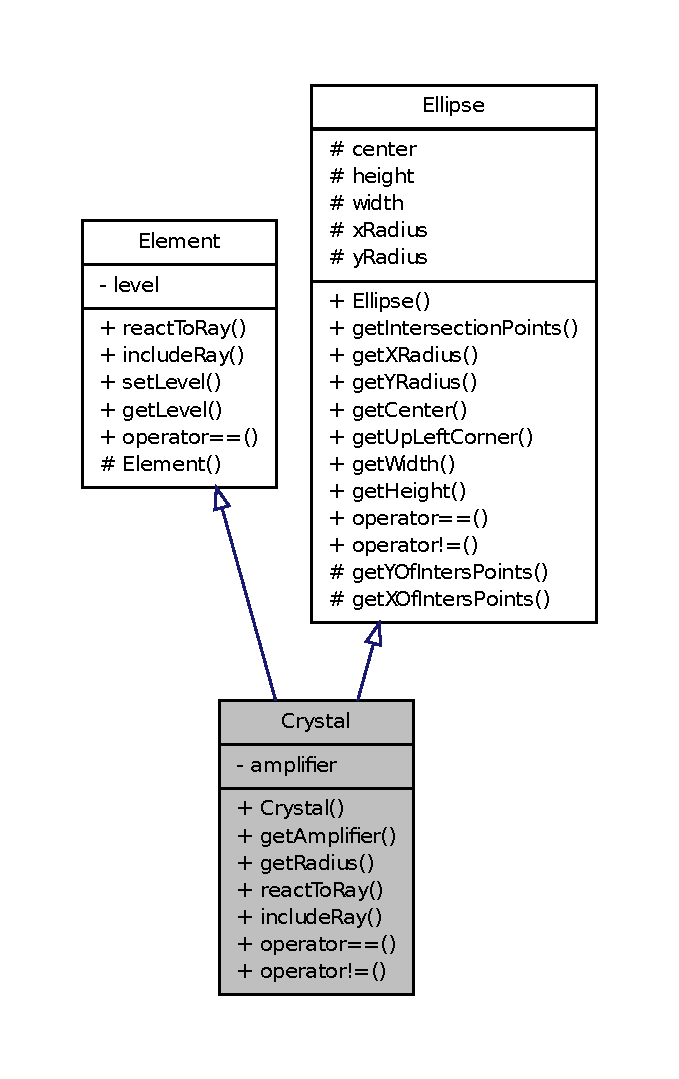
\includegraphics[width=326pt]{de/da2/classCrystal__inherit__graph}
\end{center}
\end{figure}


Graphe de collaboration de Crystal\+:\nopagebreak
\begin{figure}[H]
\begin{center}
\leavevmode
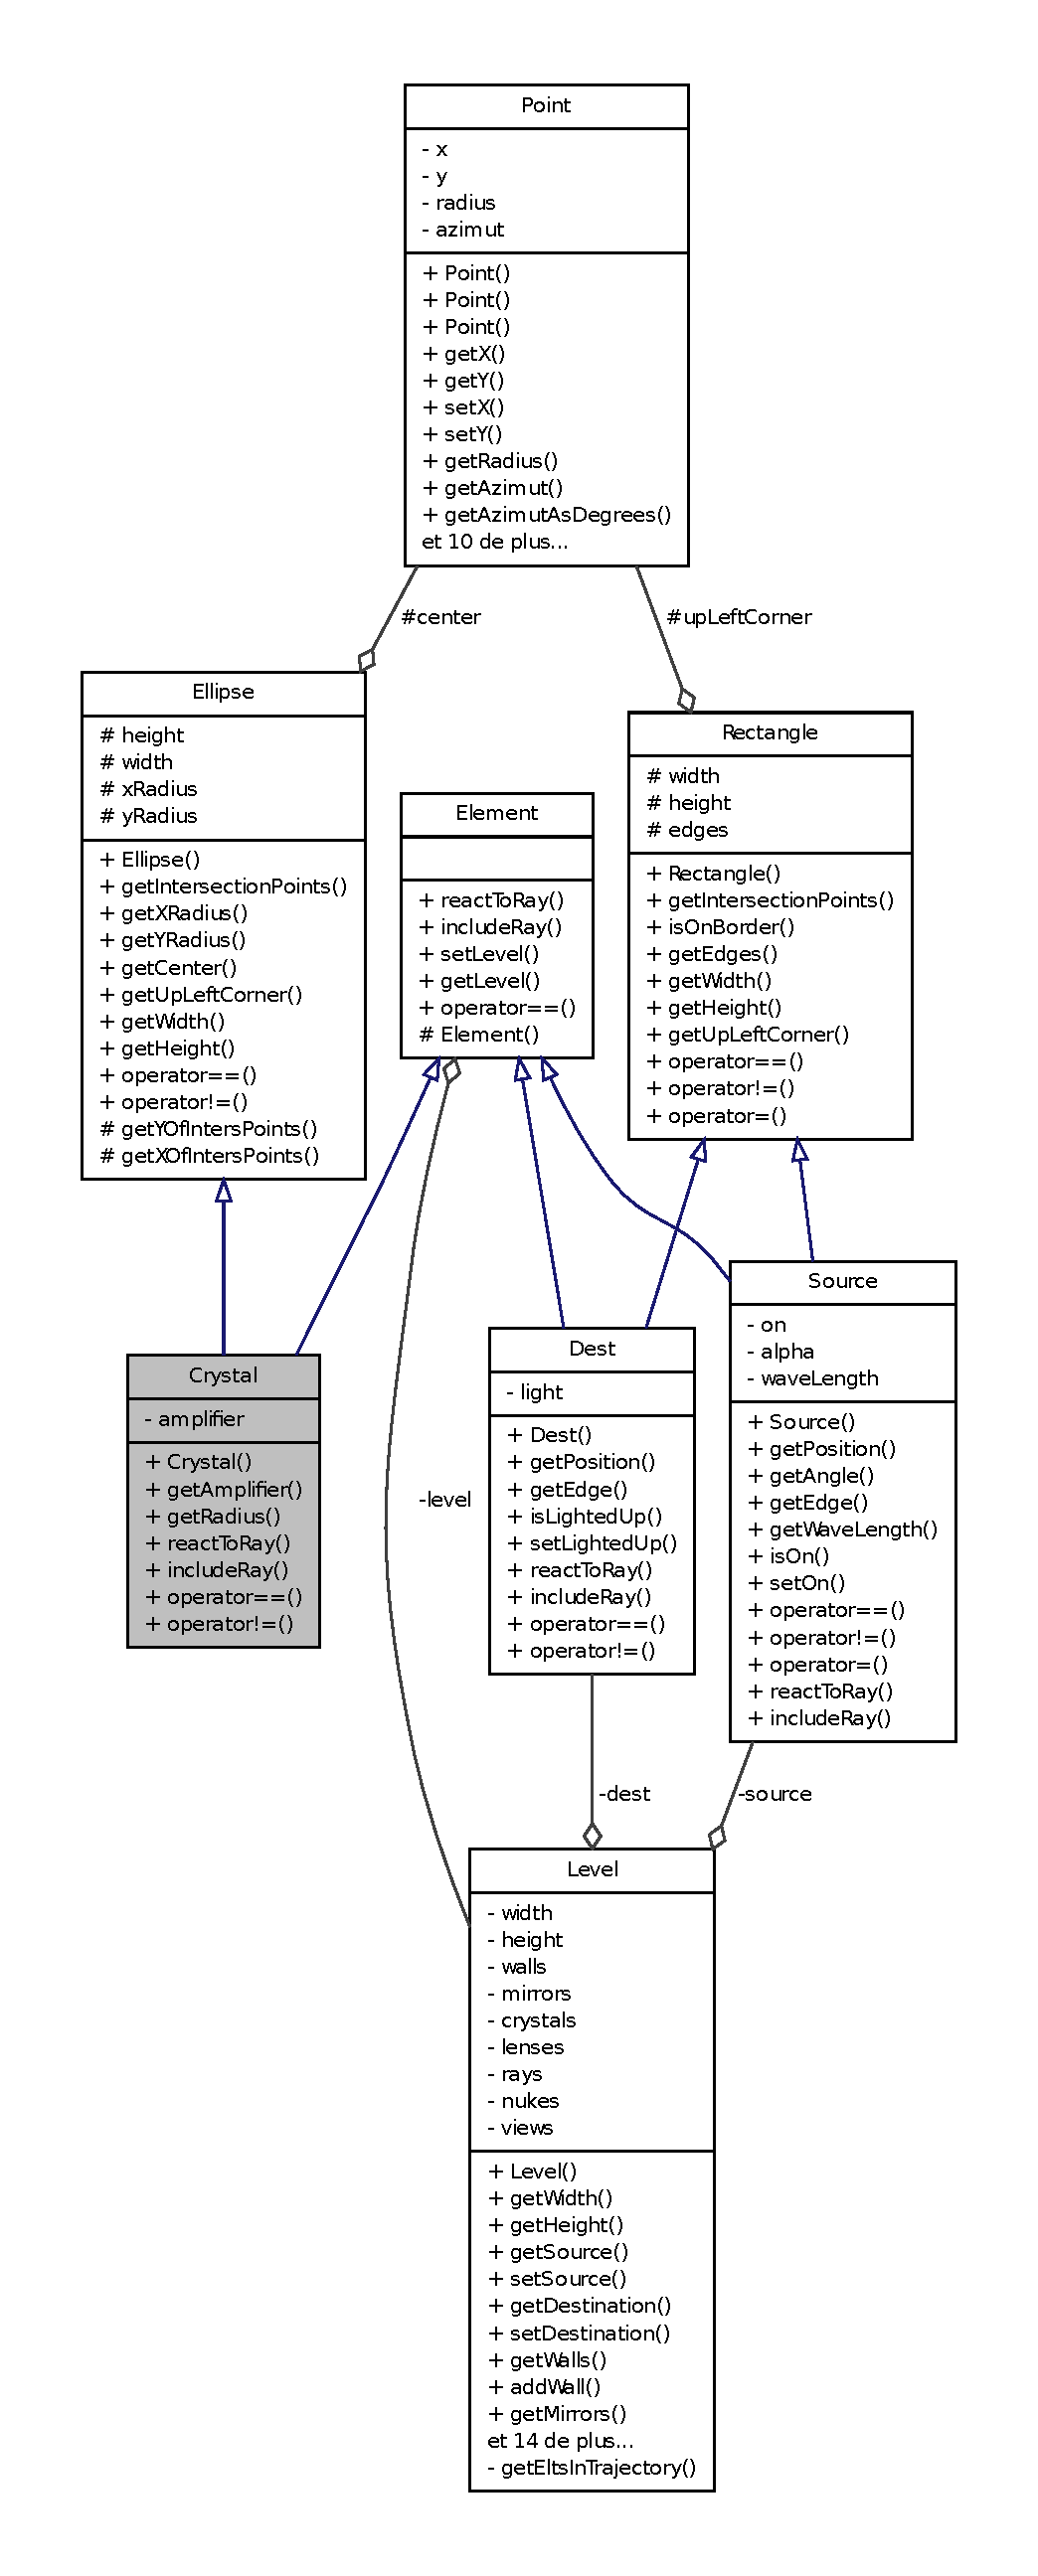
\includegraphics[height=550pt]{d4/db0/classCrystal__coll__graph}
\end{center}
\end{figure}


\subsection{Documentation des constructeurs et destructeur}
\hypertarget{classCrystal_ace23d553475cfcd48496d8c2dc1ae656}{}\index{Crystal@{Crystal}!Crystal@{Crystal}}
\index{Crystal@{Crystal}!Crystal@{Crystal}}
\subsubsection[{Crystal(const Point \&, const double, const int)}]{\setlength{\rightskip}{0pt plus 5cm}Crystal\+::\+Crystal (
\begin{DoxyParamCaption}
\item[{const {\bf Point} \&}]{, }
\item[{const double}]{, }
\item[{const int}]{}
\end{DoxyParamCaption}
)}\label{classCrystal_ace23d553475cfcd48496d8c2dc1ae656}


Instancier un cristal. 


\begin{DoxyItemize}
\item centré au point donné 
\item avec un rayon donné 
\item et un amplifier de longueur d\textquotesingle{}ondes donné 
\end{DoxyItemize},

ce crystal modifie la longueur d\textquotesingle{}onde du rayon le traversant en suivant la règle suivante \+: si la longueur d\textquotesingle{}onde modifié sort de l\textquotesingle{}intervalle \mbox{[}longueur d\textquotesingle{}onde minimale, longueur d\textquotesingle{}onde maximale\mbox{]} alors elle ne sera pas appliquée.


\begin{DoxyParams}{Paramètres}
{\em point} & Le point du centre du cristal. \\
\hline
{\em radius} & Le rayon du cristal. \\
\hline
{\em amplifieur} & le modificateur de longueur d\textquotesingle{}onde du cristal. \\
\hline
\end{DoxyParams}


\subsection{Documentation des fonctions membres}
\hypertarget{classCrystal_a231a9965f3c0651a7c0776b12e8acd37}{}\index{Crystal@{Crystal}!get\+Amplifier@{get\+Amplifier}}
\index{get\+Amplifier@{get\+Amplifier}!Crystal@{Crystal}}
\subsubsection[{get\+Amplifier() const }]{\setlength{\rightskip}{0pt plus 5cm}int Crystal\+::get\+Amplifier (
\begin{DoxyParamCaption}
{}
\end{DoxyParamCaption}
) const\hspace{0.3cm}{\ttfamily [inline]}}\label{classCrystal_a231a9965f3c0651a7c0776b12e8acd37}


Retourne le modifieur de longueur d\textquotesingle{}onde du cristal. 

\begin{DoxyReturn}{Renvoie}
le modifieur de longueur d\textquotesingle{}onde du cristal 
\end{DoxyReturn}


Définition à la ligne 110 du fichier crystal.\+hpp.



Références amplifier.


\begin{DoxyCode}
111 \{
112     \textcolor{keywordflow}{return} this->\hyperlink{classCrystal_a6732b62ec55a56f8d29249281e432cc9}{amplifier};
113 \}
\end{DoxyCode}
\hypertarget{classCrystal_a455b55c1fc7c1083a8c4dd437584ccfb}{}\index{Crystal@{Crystal}!get\+Radius@{get\+Radius}}
\index{get\+Radius@{get\+Radius}!Crystal@{Crystal}}
\subsubsection[{get\+Radius() const }]{\setlength{\rightskip}{0pt plus 5cm}double Crystal\+::get\+Radius (
\begin{DoxyParamCaption}
{}
\end{DoxyParamCaption}
) const}\label{classCrystal_a455b55c1fc7c1083a8c4dd437584ccfb}


Retourne la longueur du rayon du cristal. 

\begin{DoxyReturn}{Renvoie}
la longueur du rayon du cristal 
\end{DoxyReturn}
\hypertarget{classCrystal_a97212bbcd6c34f243ac8f18b6641e639}{}\index{Crystal@{Crystal}!include\+Ray@{include\+Ray}}
\index{include\+Ray@{include\+Ray}!Crystal@{Crystal}}
\subsubsection[{include\+Ray(const Ray \&) const }]{\setlength{\rightskip}{0pt plus 5cm}{\bf Point}$\ast$ Crystal\+::include\+Ray (
\begin{DoxyParamCaption}
\item[{const {\bf Ray} \&}]{}
\end{DoxyParamCaption}
) const\hspace{0.3cm}{\ttfamily [virtual]}}\label{classCrystal_a97212bbcd6c34f243ac8f18b6641e639}


Renseigne si le crystal est dans la trajectoire du rayon. 


\begin{DoxyParams}{Paramètres}
{\em ray} & Un rayon.\\
\hline
\end{DoxyParams}
\begin{DoxyReturn}{Renvoie}
Un pointeur vers le point d\textquotesingle{}intersection (le plus éloigné) avec le rayon s\textquotesingle{}il existe un pointeur null sinon. 
\end{DoxyReturn}


Implémente \hyperlink{classElement_a1b88519623a6250155f7182706665448}{Element}.

\hypertarget{classCrystal_aa6d486aaf4abc84b0795b75c3e3e598f}{}\index{Crystal@{Crystal}!operator"!=@{operator"!=}}
\index{operator"!=@{operator"!=}!Crystal@{Crystal}}
\subsubsection[{operator"!=(const Crystal \&) const }]{\setlength{\rightskip}{0pt plus 5cm}bool Crystal\+::operator!= (
\begin{DoxyParamCaption}
\item[{const {\bf Crystal} \&}]{}
\end{DoxyParamCaption}
) const}\label{classCrystal_aa6d486aaf4abc84b0795b75c3e3e598f}


Permet de savoir si deux cristaux sont différents. 

\begin{DoxyReturn}{Renvoie}
{\ttfamily true} si deux cristaux sont différents. 
\end{DoxyReturn}
\hypertarget{classCrystal_adeb9d4a8d0d02ff4daccd09650e1b990}{}\index{Crystal@{Crystal}!operator==@{operator==}}
\index{operator==@{operator==}!Crystal@{Crystal}}
\subsubsection[{operator==(const Crystal \&) const }]{\setlength{\rightskip}{0pt plus 5cm}bool Crystal\+::operator== (
\begin{DoxyParamCaption}
\item[{const {\bf Crystal} \&}]{}
\end{DoxyParamCaption}
) const}\label{classCrystal_adeb9d4a8d0d02ff4daccd09650e1b990}


Permet de savoir si deux cristaux sont les même. 

\begin{DoxyReturn}{Renvoie}
{\ttfamily true} si deux cristaux sont les même. 
\end{DoxyReturn}
\hypertarget{classCrystal_a4f9351f0556cf2e9334d7976bff48830}{}\index{Crystal@{Crystal}!react\+To\+Ray@{react\+To\+Ray}}
\index{react\+To\+Ray@{react\+To\+Ray}!Crystal@{Crystal}}
\subsubsection[{react\+To\+Ray(\+Ray)}]{\setlength{\rightskip}{0pt plus 5cm}void Crystal\+::react\+To\+Ray (
\begin{DoxyParamCaption}
\item[{{\bf Ray}}]{}
\end{DoxyParamCaption}
)\hspace{0.3cm}{\ttfamily [virtual]}}\label{classCrystal_a4f9351f0556cf2e9334d7976bff48830}


Cette méthode est lancé lorsque le miroir courant est exposé à un rayon. 

Il va communiquer au niveau le nouveau rayon sortant du cristal.


\begin{DoxyParams}{Paramètres}
{\em ray} & Un rayon percutant le miroir. \\
\hline
\end{DoxyParams}


Implémente \hyperlink{classElement_aa87116bb9422d64169b2ebf03831df9b}{Element}.



\subsection{Documentation des données membres}
\hypertarget{classCrystal_a6732b62ec55a56f8d29249281e432cc9}{}\index{Crystal@{Crystal}!amplifier@{amplifier}}
\index{amplifier@{amplifier}!Crystal@{Crystal}}
\subsubsection[{amplifier}]{\setlength{\rightskip}{0pt plus 5cm}int Crystal\+::amplifier\hspace{0.3cm}{\ttfamily [private]}}\label{classCrystal_a6732b62ec55a56f8d29249281e432cc9}


Le modificateur de longueur d\textquotesingle{}onde agissant sur un rayon passant dans ce cristal. 



Définition à la ligne 31 du fichier crystal.\+hpp.



Référencé par get\+Amplifier().



La documentation de cette classe a été générée à partir du fichier suivant \+:\begin{DoxyCompactItemize}
\item 
model/elements/\hyperlink{crystal_8hpp}{crystal.\+hpp}\end{DoxyCompactItemize}

\hypertarget{classDest}{}\section{Référence de la classe Dest}
\label{classDest}\index{Dest@{Dest}}


Cette classe modélise la destination utilisée dans le jeu.  




{\ttfamily \#include $<$dest.\+hpp$>$}

\subsection*{Fonctions membres publiques}
\begin{DoxyCompactItemize}
\item 
\hyperlink{classDest_a4218312bea6a7f4d12f77c938c4ee7b6}{Dest} (const \hyperlink{classPoint}{Point} \&, const int)
\begin{DoxyCompactList}\small\item\em Intancie une destination, de position et rayon donné. \end{DoxyCompactList}\item 
const \hyperlink{classPoint}{Point} \& \hyperlink{classDest_ab2d0734c1d7bb18051f4a9fd9796bbb6}{get\+Position} () const 
\begin{DoxyCompactList}\small\item\em Retourne la position du coin supérieur gauche du carré modélisant la destination. \end{DoxyCompactList}\item 
int \hyperlink{classDest_a5fdb7d4528a909d58ca79f680c99dc4a}{get\+Edge} () const 
\begin{DoxyCompactList}\small\item\em Retourne la longueur du côté du carré. \end{DoxyCompactList}\item 
bool \hyperlink{classDest_a3fe90c4d766a5a676e0d539d5ba00780}{is\+Lighted\+Up} () const 
\begin{DoxyCompactList}\small\item\em Permet de savoir si la destination est éclairée et donc si le jeu est terminé. \end{DoxyCompactList}\item 
void \hyperlink{classDest_a6b781ddf5c4d26b5439d12a928190af3}{set\+Lighted\+Up} (const bool)
\begin{DoxyCompactList}\small\item\em Permet de changer l\textquotesingle{}état d\textquotesingle{}illumination de la destination. \end{DoxyCompactList}\item 
void \hyperlink{classDest_ad4f6b777efe8d4cd277e635c2c2ee3df}{react\+To\+Ray} (\hyperlink{classRay}{Ray})
\begin{DoxyCompactList}\small\item\em Cette méthode est lancé lorsque la destination courant est exposé à un rayon. \end{DoxyCompactList}\item 
\hyperlink{classPoint}{Point} $\ast$ \hyperlink{classDest_aa0ec59799948c6a949907db4a12e2f11}{include\+Ray} (const \hyperlink{classRay}{Ray} \&) const 
\begin{DoxyCompactList}\small\item\em Renseigne si la destination est dans la trajectoire du rayon. \end{DoxyCompactList}\item 
bool \hyperlink{classDest_a0329ceede6eacadc211890bb3397197c}{operator==} (const \hyperlink{classDest}{Dest} \&) const 
\begin{DoxyCompactList}\small\item\em Permet de savoir si deux destinations sont les même. \end{DoxyCompactList}\item 
bool \hyperlink{classDest_a5d62d68ec9de0d58920a82a00ed72a53}{operator!=} (const \hyperlink{classDest}{Dest} \&) const 
\begin{DoxyCompactList}\small\item\em Permet de savoir si deux destinations sont différentes. \end{DoxyCompactList}\end{DoxyCompactItemize}
\subsection*{Attributs privés}
\begin{DoxyCompactItemize}
\item 
bool \hyperlink{classDest_abde9aa4bba2ce7868d90fa873761753d}{light}
\end{DoxyCompactItemize}
\subsection*{Membres hérités additionnels}


\subsection{Description détaillée}
Cette classe modélise la destination utilisée dans le jeu. 

Une destination est un objet carré qui, quand traversé par un rayon lumineux, fait remporter la partie au joueur. 

Définition à la ligne 17 du fichier dest.\+hpp.



Graphe d\textquotesingle{}héritage de Dest\+:\nopagebreak
\begin{figure}[H]
\begin{center}
\leavevmode
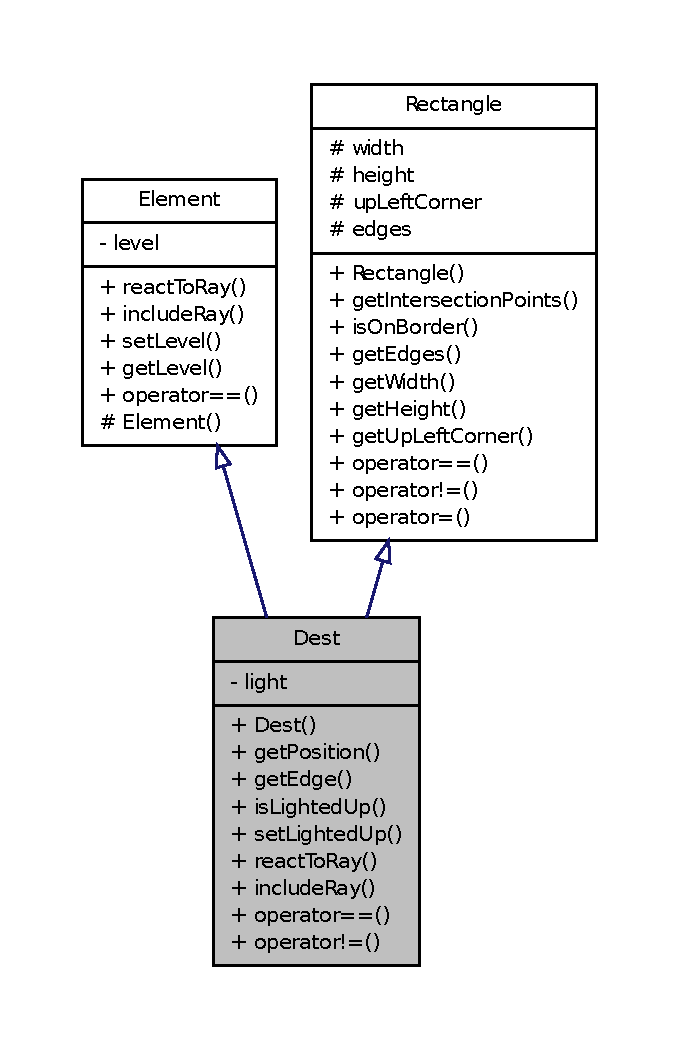
\includegraphics[width=326pt]{d9/d5c/classDest__inherit__graph}
\end{center}
\end{figure}


Graphe de collaboration de Dest\+:\nopagebreak
\begin{figure}[H]
\begin{center}
\leavevmode
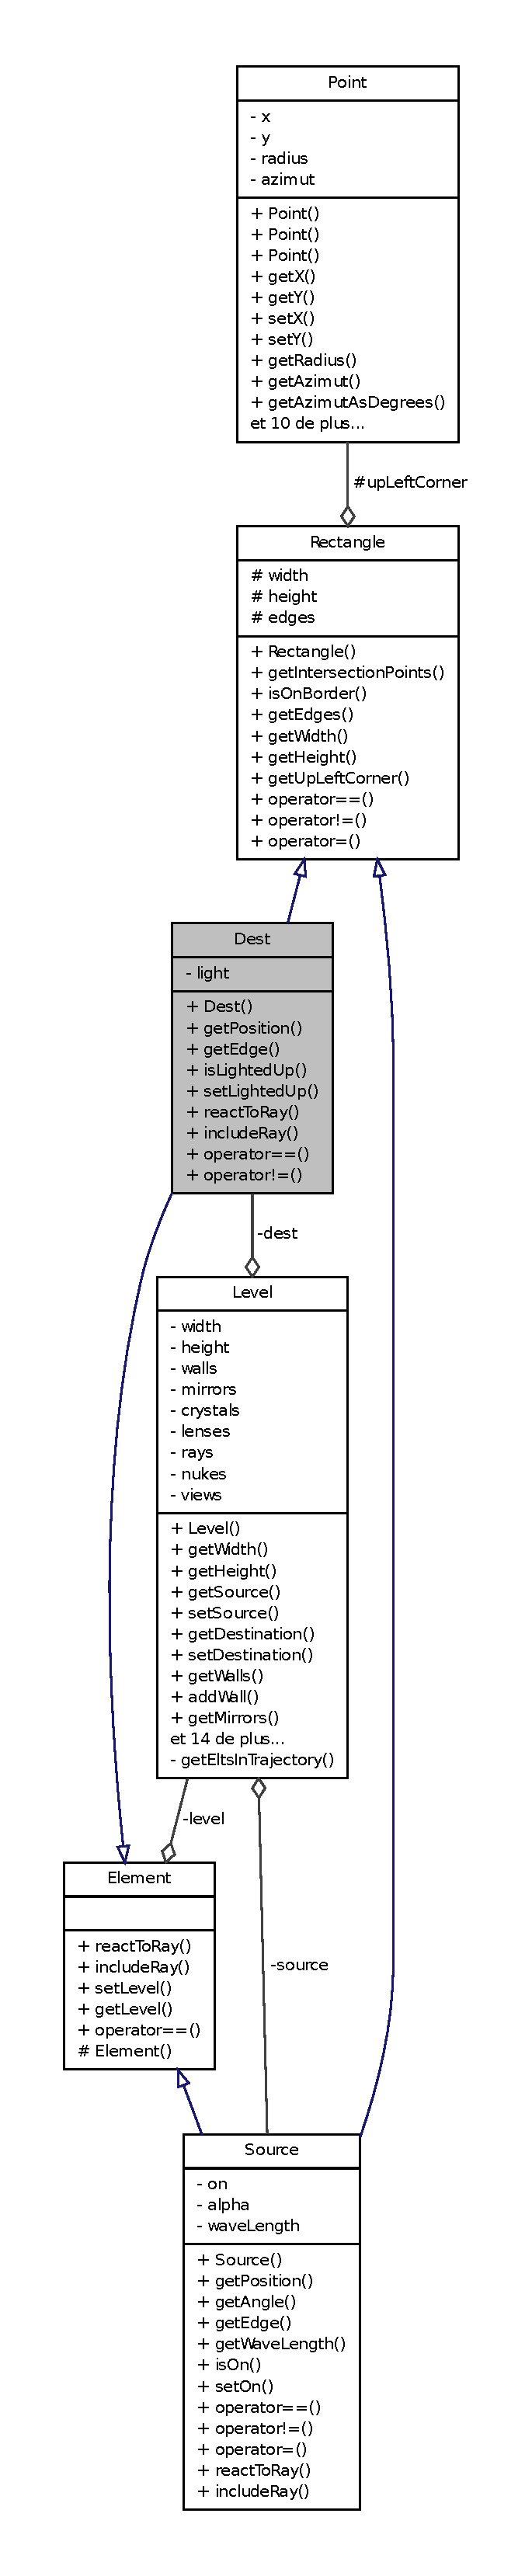
\includegraphics[height=550pt]{d4/d77/classDest__coll__graph}
\end{center}
\end{figure}


\subsection{Documentation des constructeurs et destructeur}
\hypertarget{classDest_a4218312bea6a7f4d12f77c938c4ee7b6}{}\index{Dest@{Dest}!Dest@{Dest}}
\index{Dest@{Dest}!Dest@{Dest}}
\subsubsection[{Dest(const Point \&, const int)}]{\setlength{\rightskip}{0pt plus 5cm}Dest\+::\+Dest (
\begin{DoxyParamCaption}
\item[{const {\bf Point} \&}]{, }
\item[{const int}]{}
\end{DoxyParamCaption}
)}\label{classDest_a4218312bea6a7f4d12f77c938c4ee7b6}


Intancie une destination, de position et rayon donné. 


\begin{DoxyParams}{Paramètres}
{\em position} & Le coin supérieur gauche du carré modélisant la destination. \\
\hline
{\em edge} & La longueur du côté du carré. \\
\hline
\end{DoxyParams}


\subsection{Documentation des fonctions membres}
\hypertarget{classDest_a5fdb7d4528a909d58ca79f680c99dc4a}{}\index{Dest@{Dest}!get\+Edge@{get\+Edge}}
\index{get\+Edge@{get\+Edge}!Dest@{Dest}}
\subsubsection[{get\+Edge() const }]{\setlength{\rightskip}{0pt plus 5cm}int Dest\+::get\+Edge (
\begin{DoxyParamCaption}
{}
\end{DoxyParamCaption}
) const\hspace{0.3cm}{\ttfamily [inline]}}\label{classDest_a5fdb7d4528a909d58ca79f680c99dc4a}


Retourne la longueur du côté du carré. 

\begin{DoxyReturn}{Renvoie}
La longueur du côté du carré. 
\end{DoxyReturn}


Définition à la ligne 110 du fichier dest.\+hpp.



Références Rectangle\+::height.


\begin{DoxyCode}
111 \{
112     \textcolor{keywordflow}{return} this->\hyperlink{classRectangle_a58c0573f0d706d238759395e8272c6bf}{height};
113 \}
\end{DoxyCode}
\hypertarget{classDest_ab2d0734c1d7bb18051f4a9fd9796bbb6}{}\index{Dest@{Dest}!get\+Position@{get\+Position}}
\index{get\+Position@{get\+Position}!Dest@{Dest}}
\subsubsection[{get\+Position() const }]{\setlength{\rightskip}{0pt plus 5cm}const {\bf Point} \& Dest\+::get\+Position (
\begin{DoxyParamCaption}
{}
\end{DoxyParamCaption}
) const\hspace{0.3cm}{\ttfamily [inline]}}\label{classDest_ab2d0734c1d7bb18051f4a9fd9796bbb6}


Retourne la position du coin supérieur gauche du carré modélisant la destination. 

\begin{DoxyReturn}{Renvoie}
La position de la destination. 
\end{DoxyReturn}


Définition à la ligne 105 du fichier dest.\+hpp.



Références Rectangle\+::up\+Left\+Corner.


\begin{DoxyCode}
106 \{
107     \textcolor{keywordflow}{return} this->\hyperlink{classRectangle_aeeb6ca62aa27e964265c92d1ea25d511}{upLeftCorner};
108 \}
\end{DoxyCode}
\hypertarget{classDest_aa0ec59799948c6a949907db4a12e2f11}{}\index{Dest@{Dest}!include\+Ray@{include\+Ray}}
\index{include\+Ray@{include\+Ray}!Dest@{Dest}}
\subsubsection[{include\+Ray(const Ray \&) const }]{\setlength{\rightskip}{0pt plus 5cm}{\bf Point}$\ast$ Dest\+::include\+Ray (
\begin{DoxyParamCaption}
\item[{const {\bf Ray} \&}]{}
\end{DoxyParamCaption}
) const\hspace{0.3cm}{\ttfamily [virtual]}}\label{classDest_aa0ec59799948c6a949907db4a12e2f11}


Renseigne si la destination est dans la trajectoire du rayon. 


\begin{DoxyParams}{Paramètres}
{\em ray} & Le rayon.\\
\hline
\end{DoxyParams}
\begin{DoxyReturn}{Renvoie}
{\ttfamily true} Si la destination se trouve dans la trajectoire du rayon entré en paramètre. 
\end{DoxyReturn}


Implémente \hyperlink{classElement_a1b88519623a6250155f7182706665448}{Element}.

\hypertarget{classDest_a3fe90c4d766a5a676e0d539d5ba00780}{}\index{Dest@{Dest}!is\+Lighted\+Up@{is\+Lighted\+Up}}
\index{is\+Lighted\+Up@{is\+Lighted\+Up}!Dest@{Dest}}
\subsubsection[{is\+Lighted\+Up() const }]{\setlength{\rightskip}{0pt plus 5cm}bool Dest\+::is\+Lighted\+Up (
\begin{DoxyParamCaption}
{}
\end{DoxyParamCaption}
) const\hspace{0.3cm}{\ttfamily [inline]}}\label{classDest_a3fe90c4d766a5a676e0d539d5ba00780}


Permet de savoir si la destination est éclairée et donc si le jeu est terminé. 

\begin{DoxyReturn}{Renvoie}
{\ttfamily true} Si la destination est illuminée. 
\end{DoxyReturn}


Définition à la ligne 115 du fichier dest.\+hpp.



Références light.


\begin{DoxyCode}
116 \{
117     \textcolor{keywordflow}{return} this->\hyperlink{classDest_abde9aa4bba2ce7868d90fa873761753d}{light};
118 \}
\end{DoxyCode}
\hypertarget{classDest_a5d62d68ec9de0d58920a82a00ed72a53}{}\index{Dest@{Dest}!operator"!=@{operator"!=}}
\index{operator"!=@{operator"!=}!Dest@{Dest}}
\subsubsection[{operator"!=(const Dest \&) const }]{\setlength{\rightskip}{0pt plus 5cm}bool Dest\+::operator!= (
\begin{DoxyParamCaption}
\item[{const {\bf Dest} \&}]{}
\end{DoxyParamCaption}
) const}\label{classDest_a5d62d68ec9de0d58920a82a00ed72a53}


Permet de savoir si deux destinations sont différentes. 

\begin{DoxyReturn}{Renvoie}
{\ttfamily true} Si les destinations sont différentes. 
\end{DoxyReturn}
\hypertarget{classDest_a0329ceede6eacadc211890bb3397197c}{}\index{Dest@{Dest}!operator==@{operator==}}
\index{operator==@{operator==}!Dest@{Dest}}
\subsubsection[{operator==(const Dest \&) const }]{\setlength{\rightskip}{0pt plus 5cm}bool Dest\+::operator== (
\begin{DoxyParamCaption}
\item[{const {\bf Dest} \&}]{}
\end{DoxyParamCaption}
) const}\label{classDest_a0329ceede6eacadc211890bb3397197c}


Permet de savoir si deux destinations sont les même. 

\begin{DoxyReturn}{Renvoie}
{\ttfamily true} Si les destinations sont les même. 
\end{DoxyReturn}
\hypertarget{classDest_ad4f6b777efe8d4cd277e635c2c2ee3df}{}\index{Dest@{Dest}!react\+To\+Ray@{react\+To\+Ray}}
\index{react\+To\+Ray@{react\+To\+Ray}!Dest@{Dest}}
\subsubsection[{react\+To\+Ray(\+Ray)}]{\setlength{\rightskip}{0pt plus 5cm}void Dest\+::react\+To\+Ray (
\begin{DoxyParamCaption}
\item[{{\bf Ray}}]{}
\end{DoxyParamCaption}
)\hspace{0.3cm}{\ttfamily [virtual]}}\label{classDest_ad4f6b777efe8d4cd277e635c2c2ee3df}


Cette méthode est lancé lorsque la destination courant est exposé à un rayon. 

Elle va s\textquotesingle{}exposer comme illuminée.


\begin{DoxyParams}{Paramètres}
{\em ray} & Un rayon percutant la destination. \\
\hline
\end{DoxyParams}


Implémente \hyperlink{classElement_aa87116bb9422d64169b2ebf03831df9b}{Element}.

\hypertarget{classDest_a6b781ddf5c4d26b5439d12a928190af3}{}\index{Dest@{Dest}!set\+Lighted\+Up@{set\+Lighted\+Up}}
\index{set\+Lighted\+Up@{set\+Lighted\+Up}!Dest@{Dest}}
\subsubsection[{set\+Lighted\+Up(const bool)}]{\setlength{\rightskip}{0pt plus 5cm}void Dest\+::set\+Lighted\+Up (
\begin{DoxyParamCaption}
\item[{const bool}]{}
\end{DoxyParamCaption}
)}\label{classDest_a6b781ddf5c4d26b5439d12a928190af3}


Permet de changer l\textquotesingle{}état d\textquotesingle{}illumination de la destination. 


\begin{DoxyParams}{Paramètres}
{\em Le} & nouvelle état d\textquotesingle{}illumination de la destination. \\
\hline
\end{DoxyParams}


\subsection{Documentation des données membres}
\hypertarget{classDest_abde9aa4bba2ce7868d90fa873761753d}{}\index{Dest@{Dest}!light@{light}}
\index{light@{light}!Dest@{Dest}}
\subsubsection[{light}]{\setlength{\rightskip}{0pt plus 5cm}bool Dest\+::light\hspace{0.3cm}{\ttfamily [private]}}\label{classDest_abde9aa4bba2ce7868d90fa873761753d}


Définition à la ligne 22 du fichier dest.\+hpp.



Référencé par is\+Lighted\+Up().



La documentation de cette classe a été générée à partir du fichier suivant \+:\begin{DoxyCompactItemize}
\item 
model/elements/\hyperlink{dest_8hpp}{dest.\+hpp}\end{DoxyCompactItemize}

\hypertarget{classElement}{}\section{Référence de la classe Element}
\label{classElement}\index{Element@{Element}}


Un élément est un composant du jeu se devant de communiquer son état au niveau le gérant.  




{\ttfamily \#include $<$element.\+hpp$>$}

\subsection*{Fonctions membres publiques}
\begin{DoxyCompactItemize}
\item 
virtual void \hyperlink{classElement_aa87116bb9422d64169b2ebf03831df9b}{react\+To\+Ray} (\hyperlink{classRay}{Ray})=0
\begin{DoxyCompactList}\small\item\em Réaction à l\textquotesingle{}exposition d\textquotesingle{}un rayon. \end{DoxyCompactList}\item 
virtual \hyperlink{classPoint}{Point} $\ast$ \hyperlink{classElement_a1b88519623a6250155f7182706665448}{include\+Ray} (const \hyperlink{classRay}{Ray} \&) const  =0
\begin{DoxyCompactList}\small\item\em Renseigne si l\textquotesingle{}élément est dans la trajectoire du rayon. \end{DoxyCompactList}\item 
void \hyperlink{classElement_a52d67b5af9d0e96092b7cd4c3058d17b}{set\+Level} (\hyperlink{classLevel}{Level} $\ast$)
\begin{DoxyCompactList}\small\item\em Permet de modifier le level auquel appartient l\textquotesingle{}élément. \end{DoxyCompactList}\item 
\hyperlink{classLevel}{Level} $\ast$ \hyperlink{classElement_aea3bbf40d27afdf61833f59775e488f3}{get\+Level} ()
\begin{DoxyCompactList}\small\item\em Permet d\textquotesingle{}obtenir un pointeur sur le niveau auquel appartient l\textquotesingle{}élément. \end{DoxyCompactList}\item 
bool \hyperlink{classElement_aa8ab9ae8d680e81c964f0eaee2dfb44d}{operator==} (const \hyperlink{classElement}{Element} \&) const 
\begin{DoxyCompactList}\small\item\em Compare deux éléments pour savoir si ils pointent vers le même niveau. \end{DoxyCompactList}\end{DoxyCompactItemize}
\subsection*{Fonctions membres protégées}
\begin{DoxyCompactItemize}
\item 
\hyperlink{classElement_a084081001b0f14ae12d612c866df861c}{Element} ()=default
\begin{DoxyCompactList}\small\item\em Constructeur par défaut, en visibilité protected permettant d\textquotesingle{}éviter une tentative d\textquotesingle{}instanciation de cette classe abstraite. \end{DoxyCompactList}\end{DoxyCompactItemize}
\subsection*{Attributs privés}
\begin{DoxyCompactItemize}
\item 
\hyperlink{classLevel}{Level} $\ast$ \hyperlink{classElement_a28c0ab6e211fb16fc2957024ca2761cb}{level} \{nullptr\}
\begin{DoxyCompactList}\small\item\em Le niveau lié à un élément. \end{DoxyCompactList}\end{DoxyCompactItemize}


\subsection{Description détaillée}
Un élément est un composant du jeu se devant de communiquer son état au niveau le gérant. 

Cette pratique permet au niveau d\textquotesingle{}écouter les actions à éffectuer dicter par l\textquotesingle{}élément. 

Définition à la ligne 13 du fichier element.\+hpp.



Graphe d\textquotesingle{}héritage de Element\+:\nopagebreak
\begin{figure}[H]
\begin{center}
\leavevmode
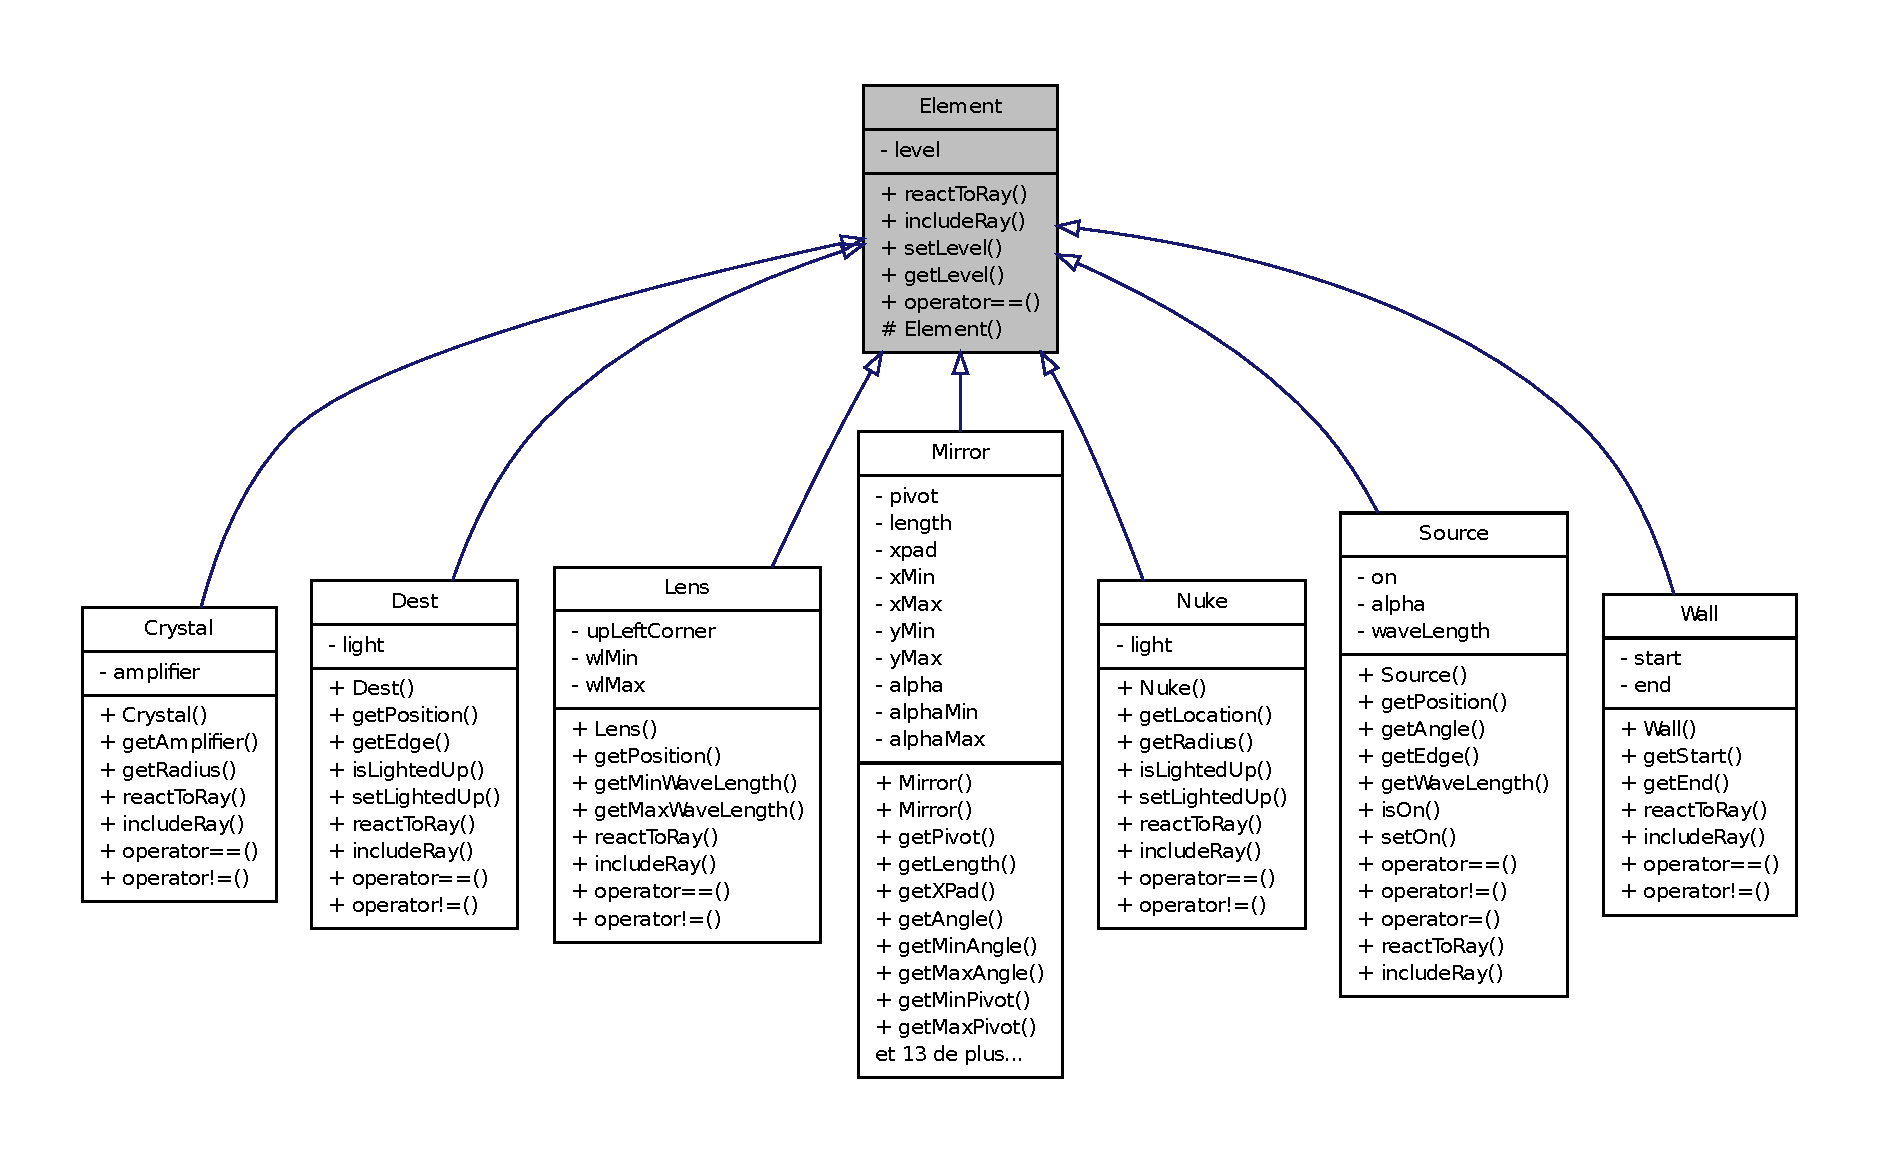
\includegraphics[width=350pt]{d8/dd6/classElement__inherit__graph}
\end{center}
\end{figure}


Graphe de collaboration de Element\+:\nopagebreak
\begin{figure}[H]
\begin{center}
\leavevmode
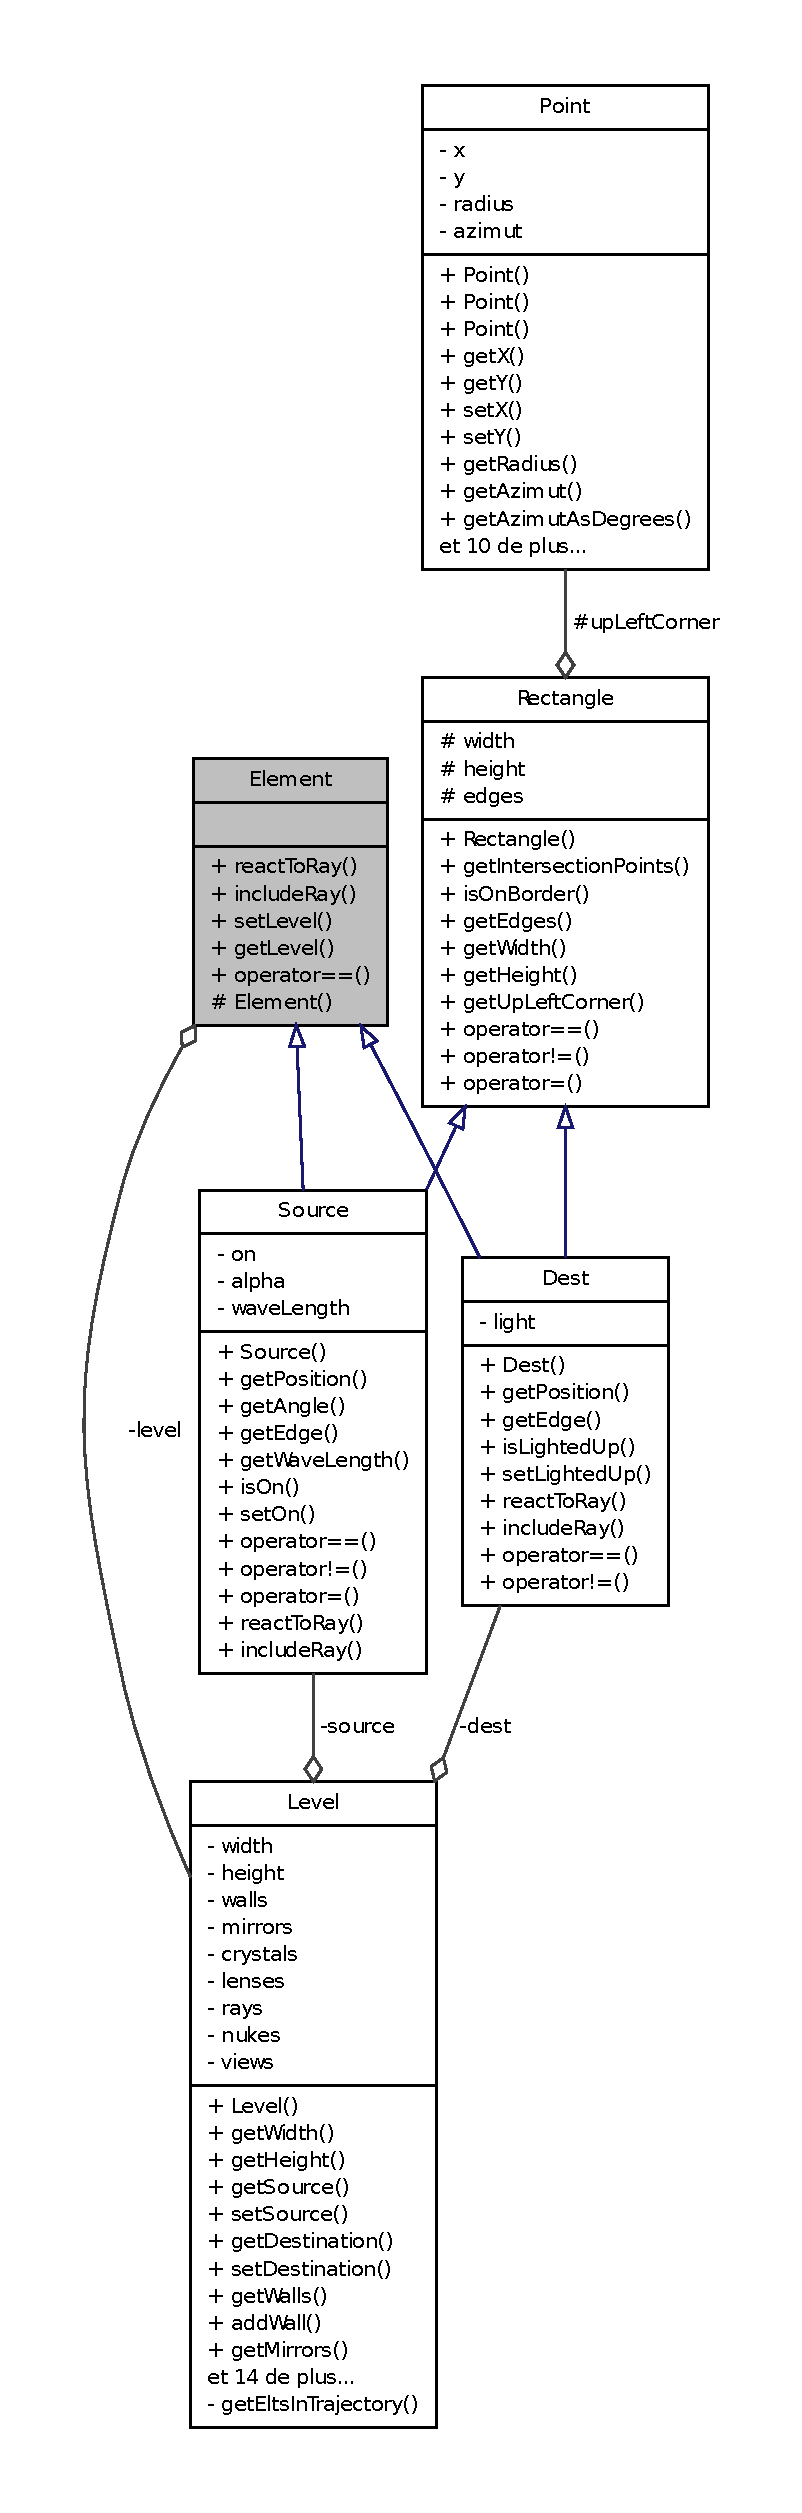
\includegraphics[height=550pt]{d4/dd1/classElement__coll__graph}
\end{center}
\end{figure}


\subsection{Documentation des constructeurs et destructeur}
\hypertarget{classElement_a084081001b0f14ae12d612c866df861c}{}\index{Element@{Element}!Element@{Element}}
\index{Element@{Element}!Element@{Element}}
\subsubsection[{Element()=default}]{\setlength{\rightskip}{0pt plus 5cm}Element\+::\+Element (
\begin{DoxyParamCaption}
{}
\end{DoxyParamCaption}
)\hspace{0.3cm}{\ttfamily [protected]}, {\ttfamily [default]}}\label{classElement_a084081001b0f14ae12d612c866df861c}


Constructeur par défaut, en visibilité protected permettant d\textquotesingle{}éviter une tentative d\textquotesingle{}instanciation de cette classe abstraite. 



\subsection{Documentation des fonctions membres}
\hypertarget{classElement_aea3bbf40d27afdf61833f59775e488f3}{}\index{Element@{Element}!get\+Level@{get\+Level}}
\index{get\+Level@{get\+Level}!Element@{Element}}
\subsubsection[{get\+Level()}]{\setlength{\rightskip}{0pt plus 5cm}{\bf Level} $\ast$ Element\+::get\+Level (
\begin{DoxyParamCaption}
{}
\end{DoxyParamCaption}
)\hspace{0.3cm}{\ttfamily [inline]}}\label{classElement_aea3bbf40d27afdf61833f59775e488f3}


Permet d\textquotesingle{}obtenir un pointeur sur le niveau auquel appartient l\textquotesingle{}élément. 

\begin{DoxyReturn}{Renvoie}
un pointeur vers le niveau auquel appartient l\textquotesingle{}élément. 
\end{DoxyReturn}


Définition à la ligne 71 du fichier element.\+hpp.



Références level.


\begin{DoxyCode}
72 \{
73     \textcolor{keywordflow}{return} this->\hyperlink{classElement_a28c0ab6e211fb16fc2957024ca2761cb}{level};
74 \}
\end{DoxyCode}
\hypertarget{classElement_a1b88519623a6250155f7182706665448}{}\index{Element@{Element}!include\+Ray@{include\+Ray}}
\index{include\+Ray@{include\+Ray}!Element@{Element}}
\subsubsection[{include\+Ray(const Ray \&) const  =0}]{\setlength{\rightskip}{0pt plus 5cm}virtual {\bf Point}$\ast$ Element\+::include\+Ray (
\begin{DoxyParamCaption}
\item[{const {\bf Ray} \&}]{}
\end{DoxyParamCaption}
) const\hspace{0.3cm}{\ttfamily [pure virtual]}}\label{classElement_a1b88519623a6250155f7182706665448}


Renseigne si l\textquotesingle{}élément est dans la trajectoire du rayon. 


\begin{DoxyParams}{Paramètres}
{\em ray} & Le rayon.\\
\hline
\end{DoxyParams}
\begin{DoxyReturn}{Renvoie}
{\ttfamily true} Si l\textquotesingle{}élément se trouve dans la trajectoire du rayon entré en paramètre. 
\end{DoxyReturn}


Implémenté dans \hyperlink{classMirror_af9b8d54ae559b388cb04df6f8d391f47}{Mirror}, \hyperlink{classSource_add4e9c5a8829777d5c522622ad31f431}{Source}, \hyperlink{classLens_a458286d40d04792b7a6db47bd9f775fc}{Lens}, \hyperlink{classCrystal_a97212bbcd6c34f243ac8f18b6641e639}{Crystal}, \hyperlink{classDest_aa0ec59799948c6a949907db4a12e2f11}{Dest}, \hyperlink{classNuke_a36dfe7d835bc760a31525898f44ff675}{Nuke}, et \hyperlink{classWall_a11178e8dc8eabc9a56b9bf5525dc4f29}{Wall}.

\hypertarget{classElement_aa8ab9ae8d680e81c964f0eaee2dfb44d}{}\index{Element@{Element}!operator==@{operator==}}
\index{operator==@{operator==}!Element@{Element}}
\subsubsection[{operator==(const Element \&) const }]{\setlength{\rightskip}{0pt plus 5cm}bool Element\+::operator== (
\begin{DoxyParamCaption}
\item[{const {\bf Element} \&}]{}
\end{DoxyParamCaption}
) const}\label{classElement_aa8ab9ae8d680e81c964f0eaee2dfb44d}


Compare deux éléments pour savoir si ils pointent vers le même niveau. 

\begin{DoxyReturn}{Renvoie}
{\ttfamily true} Si les deux éléments sont liés au même niveau. 
\end{DoxyReturn}
\hypertarget{classElement_aa87116bb9422d64169b2ebf03831df9b}{}\index{Element@{Element}!react\+To\+Ray@{react\+To\+Ray}}
\index{react\+To\+Ray@{react\+To\+Ray}!Element@{Element}}
\subsubsection[{react\+To\+Ray(\+Ray)=0}]{\setlength{\rightskip}{0pt plus 5cm}virtual void Element\+::react\+To\+Ray (
\begin{DoxyParamCaption}
\item[{{\bf Ray}}]{}
\end{DoxyParamCaption}
)\hspace{0.3cm}{\ttfamily [pure virtual]}}\label{classElement_aa87116bb9422d64169b2ebf03831df9b}


Réaction à l\textquotesingle{}exposition d\textquotesingle{}un rayon. 


\begin{DoxyParams}{Paramètres}
{\em ray} & Le rayon. \\
\hline
\end{DoxyParams}


Implémenté dans \hyperlink{classMirror_a149fb6af1dcdcffd685b21019f189c72}{Mirror}, \hyperlink{classSource_a425f400307f756ca8e39e5cfddb3d528}{Source}, \hyperlink{classLens_a3914a622c70a3c02f5f53fd33fa3340d}{Lens}, \hyperlink{classCrystal_a4f9351f0556cf2e9334d7976bff48830}{Crystal}, \hyperlink{classDest_ad4f6b777efe8d4cd277e635c2c2ee3df}{Dest}, \hyperlink{classNuke_a61433c8cba0b6e73c8c490f26bcbbe6b}{Nuke}, et \hyperlink{classWall_a4167a9d310ff17cf02d232d4f384b77d}{Wall}.

\hypertarget{classElement_a52d67b5af9d0e96092b7cd4c3058d17b}{}\index{Element@{Element}!set\+Level@{set\+Level}}
\index{set\+Level@{set\+Level}!Element@{Element}}
\subsubsection[{set\+Level(\+Level $\ast$)}]{\setlength{\rightskip}{0pt plus 5cm}void Element\+::set\+Level (
\begin{DoxyParamCaption}
\item[{{\bf Level} $\ast$}]{}
\end{DoxyParamCaption}
)}\label{classElement_a52d67b5af9d0e96092b7cd4c3058d17b}


Permet de modifier le level auquel appartient l\textquotesingle{}élément. 


\begin{DoxyParams}{Paramètres}
{\em nouveau} & level auquel appartient l\textquotesingle{}élément. \\
\hline
\end{DoxyParams}


\subsection{Documentation des données membres}
\hypertarget{classElement_a28c0ab6e211fb16fc2957024ca2761cb}{}\index{Element@{Element}!level@{level}}
\index{level@{level}!Element@{Element}}
\subsubsection[{level}]{\setlength{\rightskip}{0pt plus 5cm}{\bf Level}$\ast$ Element\+::level \{nullptr\}\hspace{0.3cm}{\ttfamily [private]}}\label{classElement_a28c0ab6e211fb16fc2957024ca2761cb}


Le niveau lié à un élément. 



Définition à la ligne 20 du fichier element.\+hpp.



Référencé par get\+Level().



La documentation de cette classe a été générée à partir du fichier suivant \+:\begin{DoxyCompactItemize}
\item 
model/elements/\hyperlink{element_8hpp}{element.\+hpp}\end{DoxyCompactItemize}

\hypertarget{classEllipse}{}\section{Référence de la classe Ellipse}
\label{classEllipse}\index{Ellipse@{Ellipse}}


Représente un cercle sous la forme; $ circle \equiv x^2/xRadius + y^2/yRadius = 1 $.  




{\ttfamily \#include $<$ellipse.\+hpp$>$}

\subsection*{Fonctions membres publiques}
\begin{DoxyCompactItemize}
\item 
\hyperlink{classEllipse_a2a12c8803bc8da1c04cd92345b7777f2}{Ellipse} (double, double, const \hyperlink{classPoint}{Point} \&)
\begin{DoxyCompactList}\small\item\em Permet de construire une nouvelle ellipse initialisée. \end{DoxyCompactList}\item 
std\+::vector$<$ \hyperlink{classPoint}{Point} $>$ \hyperlink{classEllipse_ab289196af0dafd510d44c6bb342c0f27}{get\+Intersection\+Points} (const \hyperlink{classLine}{Line} \&) const 
\begin{DoxyCompactList}\small\item\em Permet d\textquotesingle{}obtenir les points d\textquotesingle{}intersection entre le cercle et la droite entrée en paramètre. \end{DoxyCompactList}\item 
double \hyperlink{classEllipse_abbaadd47aa6c03e34ded7796afe18a26}{get\+X\+Radius} () const 
\begin{DoxyCompactList}\small\item\em Permet d\textquotesingle{}obtenir la valeur du ratio de largeur de l\textquotesingle{}ellipse. \end{DoxyCompactList}\item 
double \hyperlink{classEllipse_a984b6d3bde72676afca7889f90d5eedd}{get\+Y\+Radius} () const 
\begin{DoxyCompactList}\small\item\em Permet d\textquotesingle{}obtenir la valeur du ratio de hauteur de l\textquotesingle{}ellipse. \end{DoxyCompactList}\item 
\hyperlink{classPoint}{Point} \hyperlink{classEllipse_ab2c87589547fef01242fc0b8eb8de4f6}{get\+Center} () const 
\begin{DoxyCompactList}\small\item\em Permet d\textquotesingle{}obtenir le centre de l\textquotesingle{}ellipse. \end{DoxyCompactList}\item 
\hyperlink{classPoint}{Point} \hyperlink{classEllipse_a39cf837aa97029fb3aef3e769586c084}{get\+Up\+Left\+Corner} () const 
\begin{DoxyCompactList}\small\item\em Permet d\textquotesingle{}obtenir le coin supérieur gauche du rectangle entourant l\textquotesingle{}ellipse. \end{DoxyCompactList}\item 
double \hyperlink{classEllipse_a1aad73090801cc4b60b8c1508095ccf5}{get\+Width} () const 
\begin{DoxyCompactList}\small\item\em Permet d\textquotesingle{}obtenir la largeur de l\textquotesingle{}ellipse. \end{DoxyCompactList}\item 
double \hyperlink{classEllipse_aafb4efaa85efaf59e553c7423aa47b37}{get\+Height} () const 
\begin{DoxyCompactList}\small\item\em Permet d\textquotesingle{}obtenir la hauteur de l\textquotesingle{}ellipse. \end{DoxyCompactList}\item 
bool \hyperlink{classEllipse_ac06ebff3c587e85f15ca6f5f754bb35e}{operator==} (const \hyperlink{classEllipse}{Ellipse} \&) const 
\begin{DoxyCompactList}\small\item\em Permet de savoir si deux \hyperlink{classEllipse}{Ellipse} sont les mêmes. \end{DoxyCompactList}\item 
bool \hyperlink{classEllipse_a06f16be297b055c46f6ede471ea6ffad}{operator!=} (const \hyperlink{classEllipse}{Ellipse} \&) const 
\begin{DoxyCompactList}\small\item\em Permet de savoir si deux \hyperlink{classEllipse}{Ellipse} sont différentes. \end{DoxyCompactList}\end{DoxyCompactItemize}
\subsection*{Fonctions membres protégées}
\begin{DoxyCompactItemize}
\item 
bool \hyperlink{classEllipse_a00f04c68837ae5b89049074821576458}{get\+Y\+Of\+Inters\+Points} (const double, double $\ast$, double $\ast$) const 
\begin{DoxyCompactList}\small\item\em Permet d\textquotesingle{}obtenir les valeurs des ordonnées des points d\textquotesingle{}intersection entre l\textquotesingle{}ellipse et une droite verticale dont l\textquotesingle{}abscisse est entrée en paramètre. \end{DoxyCompactList}\item 
bool \hyperlink{classEllipse_ab1aac4ab1ea77795131ea2644963910b}{get\+X\+Of\+Inters\+Points} (const double, const double, double $\ast$, double $\ast$) const 
\begin{DoxyCompactList}\small\item\em Permet d\textquotesingle{}obtenir les abscisses des points d\textquotesingle{}intersection entre une droite non-\/verticale dont la pente et le terme indépendant de l\textquotesingle{}équation sont entrés en paramètre. \end{DoxyCompactList}\end{DoxyCompactItemize}
\subsection*{Attributs protégés}
\begin{DoxyCompactItemize}
\item 
\hyperlink{classPoint}{Point} \hyperlink{classEllipse_a88b27657adf698fded3a36fd97f90190}{center}
\begin{DoxyCompactList}\small\item\em La position du centre de l\textquotesingle{}ellipse. \end{DoxyCompactList}\item 
double \hyperlink{classEllipse_a549345caaff869f7eef31c800e37dd38}{height}
\begin{DoxyCompactList}\small\item\em La hauteur du rectangle circonscrit à l\textquotesingle{}ellipse. \end{DoxyCompactList}\item 
double \hyperlink{classEllipse_a4f2fb4b634a1c37666a0f8419c4f6d39}{width}
\begin{DoxyCompactList}\small\item\em La largeur du rectangle circonscrit à l\textquotesingle{}ellipse. \end{DoxyCompactList}\item 
double \hyperlink{classEllipse_a8e0e2fa0f3200a997f4b0567e588c823}{x\+Radius}
\begin{DoxyCompactList}\small\item\em La valeur de la demi hauteur au carré. \end{DoxyCompactList}\item 
double \hyperlink{classEllipse_a83614d1aaa446b1f8e404b6bc3cc8c19}{y\+Radius}
\begin{DoxyCompactList}\small\item\em La valeur de la demi largeur au carré. \end{DoxyCompactList}\end{DoxyCompactItemize}


\subsection{Description détaillée}
Représente un cercle sous la forme; $ circle \equiv x^2/xRadius + y^2/yRadius = 1 $. 

Définition à la ligne 15 du fichier ellipse.\+hpp.



Graphe d\textquotesingle{}héritage de Ellipse\+:\nopagebreak
\begin{figure}[H]
\begin{center}
\leavevmode
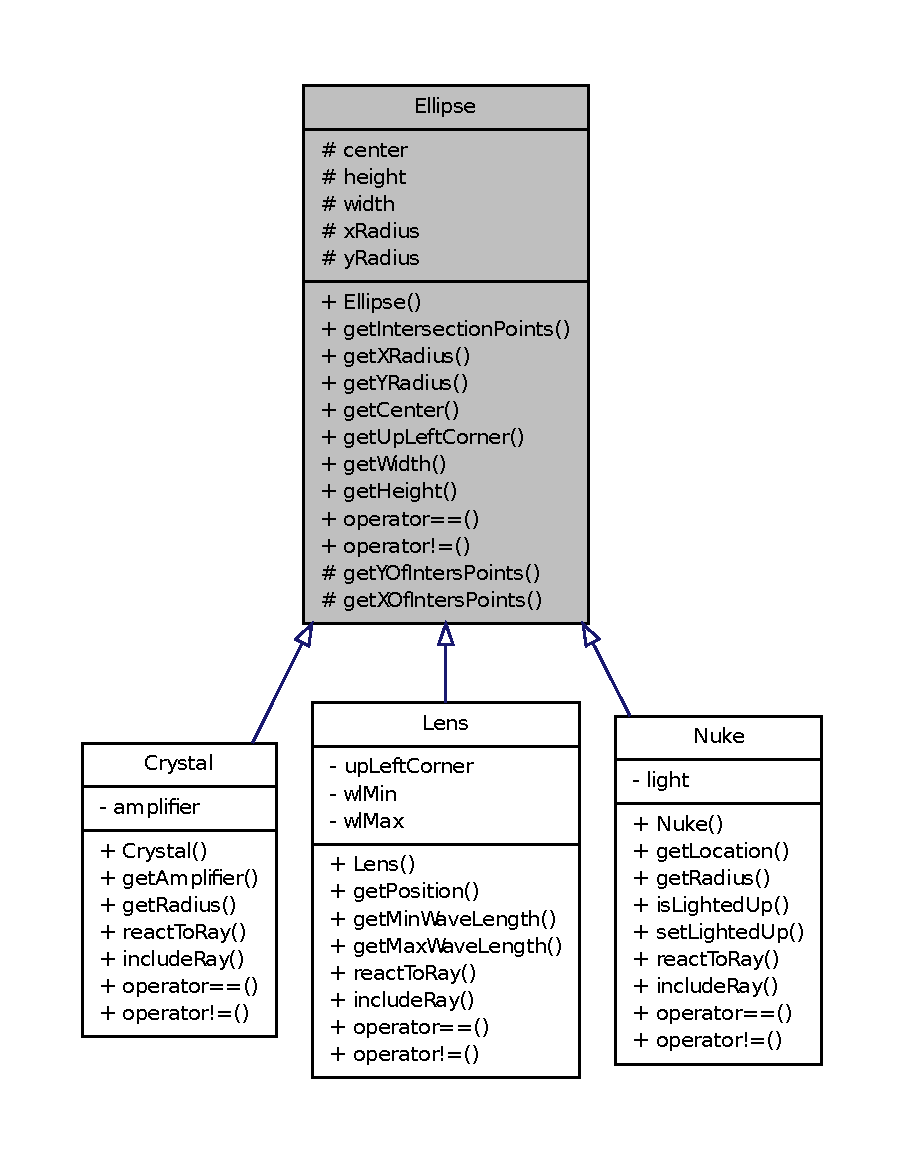
\includegraphics[width=350pt]{dd/d77/classEllipse__inherit__graph}
\end{center}
\end{figure}


Graphe de collaboration de Ellipse\+:\nopagebreak
\begin{figure}[H]
\begin{center}
\leavevmode
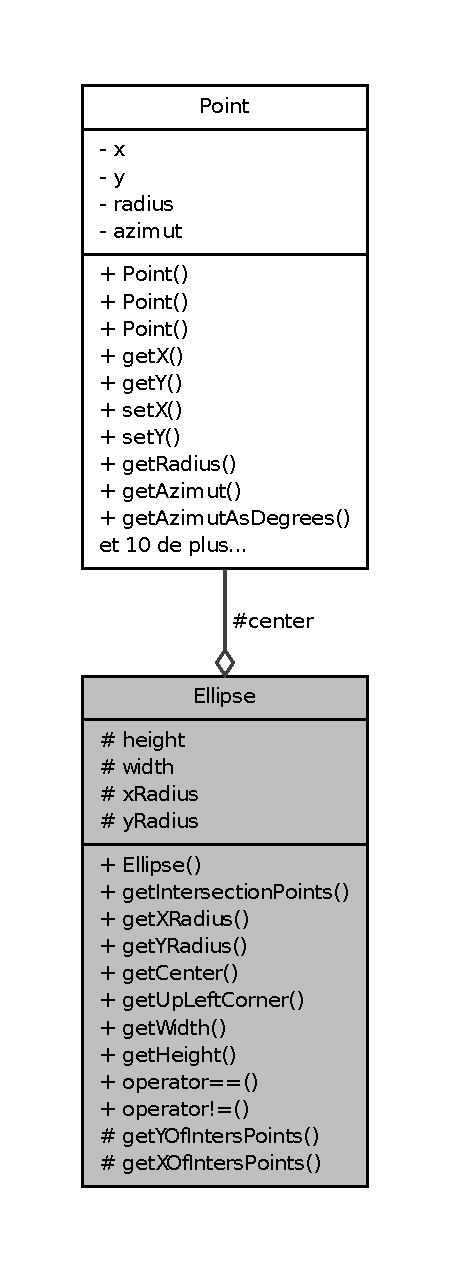
\includegraphics[height=550pt]{da/d2b/classEllipse__coll__graph}
\end{center}
\end{figure}


\subsection{Documentation des constructeurs et destructeur}
\hypertarget{classEllipse_a2a12c8803bc8da1c04cd92345b7777f2}{}\index{Ellipse@{Ellipse}!Ellipse@{Ellipse}}
\index{Ellipse@{Ellipse}!Ellipse@{Ellipse}}
\subsubsection[{Ellipse(double, double, const Point \&)}]{\setlength{\rightskip}{0pt plus 5cm}Ellipse\+::\+Ellipse (
\begin{DoxyParamCaption}
\item[{double}]{, }
\item[{double}]{, }
\item[{const {\bf Point} \&}]{}
\end{DoxyParamCaption}
)}\label{classEllipse_a2a12c8803bc8da1c04cd92345b7777f2}


Permet de construire une nouvelle ellipse initialisée. 


\begin{DoxyParams}{Paramètres}
{\em x\+Radius} & Valeur du ratio de largeur de l\textquotesingle{}ellipse. \\
\hline
{\em y\+Radius} & Valeur du ratio de hauteur de l\textquotesingle{}ellipse. \\
\hline
{\em center} & \hyperlink{classPoint}{Point} du centre de l\textquotesingle{}ellipse. \\
\hline
\end{DoxyParams}


\subsection{Documentation des fonctions membres}
\hypertarget{classEllipse_ab2c87589547fef01242fc0b8eb8de4f6}{}\index{Ellipse@{Ellipse}!get\+Center@{get\+Center}}
\index{get\+Center@{get\+Center}!Ellipse@{Ellipse}}
\subsubsection[{get\+Center() const }]{\setlength{\rightskip}{0pt plus 5cm}{\bf Point} Ellipse\+::get\+Center (
\begin{DoxyParamCaption}
{}
\end{DoxyParamCaption}
) const\hspace{0.3cm}{\ttfamily [inline]}}\label{classEllipse_ab2c87589547fef01242fc0b8eb8de4f6}


Permet d\textquotesingle{}obtenir le centre de l\textquotesingle{}ellipse. 

\begin{DoxyReturn}{Renvoie}
Le centre de l\textquotesingle{}ellipse. 
\end{DoxyReturn}


Définition à la ligne 192 du fichier ellipse.\+hpp.



Références center.


\begin{DoxyCode}
193 \{
194     \textcolor{keywordflow}{return} this->\hyperlink{classEllipse_a88b27657adf698fded3a36fd97f90190}{center};
195 \}
\end{DoxyCode}
\hypertarget{classEllipse_aafb4efaa85efaf59e553c7423aa47b37}{}\index{Ellipse@{Ellipse}!get\+Height@{get\+Height}}
\index{get\+Height@{get\+Height}!Ellipse@{Ellipse}}
\subsubsection[{get\+Height() const }]{\setlength{\rightskip}{0pt plus 5cm}double Ellipse\+::get\+Height (
\begin{DoxyParamCaption}
{}
\end{DoxyParamCaption}
) const\hspace{0.3cm}{\ttfamily [inline]}}\label{classEllipse_aafb4efaa85efaf59e553c7423aa47b37}


Permet d\textquotesingle{}obtenir la hauteur de l\textquotesingle{}ellipse. 

\begin{DoxyReturn}{Renvoie}
La hauteur de l\textquotesingle{}ellipse. 
\end{DoxyReturn}


Définition à la ligne 177 du fichier ellipse.\+hpp.



Références height.



Référencé par Nuke\+::get\+Radius().


\begin{DoxyCode}
178 \{
179     \textcolor{keywordflow}{return} this->\hyperlink{classEllipse_a549345caaff869f7eef31c800e37dd38}{height};
180 \}
\end{DoxyCode}
\hypertarget{classEllipse_ab289196af0dafd510d44c6bb342c0f27}{}\index{Ellipse@{Ellipse}!get\+Intersection\+Points@{get\+Intersection\+Points}}
\index{get\+Intersection\+Points@{get\+Intersection\+Points}!Ellipse@{Ellipse}}
\subsubsection[{get\+Intersection\+Points(const Line \&) const }]{\setlength{\rightskip}{0pt plus 5cm}std\+::vector$<${\bf Point}$>$ Ellipse\+::get\+Intersection\+Points (
\begin{DoxyParamCaption}
\item[{const {\bf Line} \&}]{}
\end{DoxyParamCaption}
) const}\label{classEllipse_ab289196af0dafd510d44c6bb342c0f27}


Permet d\textquotesingle{}obtenir les points d\textquotesingle{}intersection entre le cercle et la droite entrée en paramètre. 


\begin{DoxyParams}{Paramètres}
{\em line} & droite dont on désire obtenir les points d\textquotesingle{}intersection avec l\textquotesingle{}éllipse.\\
\hline
\end{DoxyParams}
\begin{DoxyReturn}{Renvoie}
Un vecteur contenant les points d\textquotesingle{}intersections entre le cercle et la droite entrée en paramètre. 
\end{DoxyReturn}
\hypertarget{classEllipse_a39cf837aa97029fb3aef3e769586c084}{}\index{Ellipse@{Ellipse}!get\+Up\+Left\+Corner@{get\+Up\+Left\+Corner}}
\index{get\+Up\+Left\+Corner@{get\+Up\+Left\+Corner}!Ellipse@{Ellipse}}
\subsubsection[{get\+Up\+Left\+Corner() const }]{\setlength{\rightskip}{0pt plus 5cm}{\bf Point} Ellipse\+::get\+Up\+Left\+Corner (
\begin{DoxyParamCaption}
{}
\end{DoxyParamCaption}
) const}\label{classEllipse_a39cf837aa97029fb3aef3e769586c084}


Permet d\textquotesingle{}obtenir le coin supérieur gauche du rectangle entourant l\textquotesingle{}ellipse. 

\begin{DoxyReturn}{Renvoie}
le coin supérieur gauche du rectangle entourant l\textquotesingle{}ellipse. 
\end{DoxyReturn}
\hypertarget{classEllipse_a1aad73090801cc4b60b8c1508095ccf5}{}\index{Ellipse@{Ellipse}!get\+Width@{get\+Width}}
\index{get\+Width@{get\+Width}!Ellipse@{Ellipse}}
\subsubsection[{get\+Width() const }]{\setlength{\rightskip}{0pt plus 5cm}double Ellipse\+::get\+Width (
\begin{DoxyParamCaption}
{}
\end{DoxyParamCaption}
) const\hspace{0.3cm}{\ttfamily [inline]}}\label{classEllipse_a1aad73090801cc4b60b8c1508095ccf5}


Permet d\textquotesingle{}obtenir la largeur de l\textquotesingle{}ellipse. 

\begin{DoxyReturn}{Renvoie}
La largeur de l\textquotesingle{}ellipse. 
\end{DoxyReturn}


Définition à la ligne 172 du fichier ellipse.\+hpp.



Références width.


\begin{DoxyCode}
173 \{
174     \textcolor{keywordflow}{return} this->\hyperlink{classEllipse_a4f2fb4b634a1c37666a0f8419c4f6d39}{width};
175 \}
\end{DoxyCode}
\hypertarget{classEllipse_ab1aac4ab1ea77795131ea2644963910b}{}\index{Ellipse@{Ellipse}!get\+X\+Of\+Inters\+Points@{get\+X\+Of\+Inters\+Points}}
\index{get\+X\+Of\+Inters\+Points@{get\+X\+Of\+Inters\+Points}!Ellipse@{Ellipse}}
\subsubsection[{get\+X\+Of\+Inters\+Points(const double, const double, double $\ast$, double $\ast$) const }]{\setlength{\rightskip}{0pt plus 5cm}bool Ellipse\+::get\+X\+Of\+Inters\+Points (
\begin{DoxyParamCaption}
\item[{const double}]{, }
\item[{const double}]{, }
\item[{double $\ast$}]{, }
\item[{double $\ast$}]{}
\end{DoxyParamCaption}
) const\hspace{0.3cm}{\ttfamily [protected]}}\label{classEllipse_ab1aac4ab1ea77795131ea2644963910b}


Permet d\textquotesingle{}obtenir les abscisses des points d\textquotesingle{}intersection entre une droite non-\/verticale dont la pente et le terme indépendant de l\textquotesingle{}équation sont entrés en paramètre. 


\begin{DoxyParams}{Paramètres}
{\em slope} & Pente de la droite dont on désire les abscisses des points d\textquotesingle{}intersection avec l\textquotesingle{}ellipse. \\
\hline
{\em line\+I\+T} & Terme indépendant de l\textquotesingle{}équation de la droite dont on désire les abscisses des points d\textquotesingle{}intersection avec l\textquotesingle{}ellipse. \\
\hline
{\em x1} & Conteneur de la valeur de l\textquotesingle{}abscisse du premier point d\textquotesingle{}intersection (non utilisé s\textquotesingle{}il n\textquotesingle{}existe pas de point d\textquotesingle{}intersection). \\
\hline
{\em x2} & Conteneur de la valeur de l\textquotesingle{}abscisse du deuxième point d\textquotesingle{}intersection (non utilisé s\textquotesingle{}il n\textquotesingle{}existe pas de point d\textquotesingle{}intersection).\\
\hline
\end{DoxyParams}
\begin{DoxyReturn}{Renvoie}
{\ttfamily true} Si il existe des points d\textquotesingle{}intersection entre la droite et l\textquotesingle{}ellipse. 
\end{DoxyReturn}
\hypertarget{classEllipse_abbaadd47aa6c03e34ded7796afe18a26}{}\index{Ellipse@{Ellipse}!get\+X\+Radius@{get\+X\+Radius}}
\index{get\+X\+Radius@{get\+X\+Radius}!Ellipse@{Ellipse}}
\subsubsection[{get\+X\+Radius() const }]{\setlength{\rightskip}{0pt plus 5cm}double Ellipse\+::get\+X\+Radius (
\begin{DoxyParamCaption}
{}
\end{DoxyParamCaption}
) const\hspace{0.3cm}{\ttfamily [inline]}}\label{classEllipse_abbaadd47aa6c03e34ded7796afe18a26}


Permet d\textquotesingle{}obtenir la valeur du ratio de largeur de l\textquotesingle{}ellipse. 

\begin{DoxyReturn}{Renvoie}
La valeur du ratio de largeur de l\textquotesingle{}ellipse. 
\end{DoxyReturn}


Définition à la ligne 182 du fichier ellipse.\+hpp.



Références x\+Radius.


\begin{DoxyCode}
183 \{
184     \textcolor{keywordflow}{return} this->\hyperlink{classEllipse_a8e0e2fa0f3200a997f4b0567e588c823}{xRadius};
185 \}
\end{DoxyCode}
\hypertarget{classEllipse_a00f04c68837ae5b89049074821576458}{}\index{Ellipse@{Ellipse}!get\+Y\+Of\+Inters\+Points@{get\+Y\+Of\+Inters\+Points}}
\index{get\+Y\+Of\+Inters\+Points@{get\+Y\+Of\+Inters\+Points}!Ellipse@{Ellipse}}
\subsubsection[{get\+Y\+Of\+Inters\+Points(const double, double $\ast$, double $\ast$) const }]{\setlength{\rightskip}{0pt plus 5cm}bool Ellipse\+::get\+Y\+Of\+Inters\+Points (
\begin{DoxyParamCaption}
\item[{const double}]{, }
\item[{double $\ast$}]{, }
\item[{double $\ast$}]{}
\end{DoxyParamCaption}
) const\hspace{0.3cm}{\ttfamily [protected]}}\label{classEllipse_a00f04c68837ae5b89049074821576458}


Permet d\textquotesingle{}obtenir les valeurs des ordonnées des points d\textquotesingle{}intersection entre l\textquotesingle{}ellipse et une droite verticale dont l\textquotesingle{}abscisse est entrée en paramètre. 


\begin{DoxyParams}{Paramètres}
{\em x\+Value} & Abscisse de la droite verticale dont on désire les ordonnées des points d\textquotesingle{}intersection avec l\textquotesingle{}ellipse. \\
\hline
{\em y1} & Conteneur de la valeur de l\textquotesingle{}ordonnée du premier point d\textquotesingle{}intersection (non utilisé s\textquotesingle{}il n\textquotesingle{}existe pas de point d\textquotesingle{}intersection). \\
\hline
{\em y2} & Conteneur de la valeur de l\textquotesingle{}ordonne du deuxième point d\textquotesingle{}intersection (non utilisé s\textquotesingle{}il n\textquotesingle{}existe pas de point d\textquotesingle{}intersection).\\
\hline
\end{DoxyParams}
\begin{DoxyReturn}{Renvoie}
{\ttfamily true} Si il existe des points d\textquotesingle{}intersection entre la droite et l\textquotesingle{}éllipse. 
\end{DoxyReturn}
\hypertarget{classEllipse_a984b6d3bde72676afca7889f90d5eedd}{}\index{Ellipse@{Ellipse}!get\+Y\+Radius@{get\+Y\+Radius}}
\index{get\+Y\+Radius@{get\+Y\+Radius}!Ellipse@{Ellipse}}
\subsubsection[{get\+Y\+Radius() const }]{\setlength{\rightskip}{0pt plus 5cm}double Ellipse\+::get\+Y\+Radius (
\begin{DoxyParamCaption}
{}
\end{DoxyParamCaption}
) const\hspace{0.3cm}{\ttfamily [inline]}}\label{classEllipse_a984b6d3bde72676afca7889f90d5eedd}


Permet d\textquotesingle{}obtenir la valeur du ratio de hauteur de l\textquotesingle{}ellipse. 

\begin{DoxyReturn}{Renvoie}
La valeur du ratio de hauteur de l\textquotesingle{}ellipse. 
\end{DoxyReturn}


Définition à la ligne 187 du fichier ellipse.\+hpp.



Références y\+Radius.


\begin{DoxyCode}
188 \{
189     \textcolor{keywordflow}{return} this->\hyperlink{classEllipse_a83614d1aaa446b1f8e404b6bc3cc8c19}{yRadius};
190 \}
\end{DoxyCode}
\hypertarget{classEllipse_a06f16be297b055c46f6ede471ea6ffad}{}\index{Ellipse@{Ellipse}!operator"!=@{operator"!=}}
\index{operator"!=@{operator"!=}!Ellipse@{Ellipse}}
\subsubsection[{operator"!=(const Ellipse \&) const }]{\setlength{\rightskip}{0pt plus 5cm}bool Ellipse\+::operator!= (
\begin{DoxyParamCaption}
\item[{const {\bf Ellipse} \&}]{}
\end{DoxyParamCaption}
) const}\label{classEllipse_a06f16be297b055c46f6ede471ea6ffad}


Permet de savoir si deux \hyperlink{classEllipse}{Ellipse} sont différentes. 

\begin{DoxyReturn}{Renvoie}
{\ttfamily true} Si deux Ellipses sont différentes. 
\end{DoxyReturn}
\hypertarget{classEllipse_ac06ebff3c587e85f15ca6f5f754bb35e}{}\index{Ellipse@{Ellipse}!operator==@{operator==}}
\index{operator==@{operator==}!Ellipse@{Ellipse}}
\subsubsection[{operator==(const Ellipse \&) const }]{\setlength{\rightskip}{0pt plus 5cm}bool Ellipse\+::operator== (
\begin{DoxyParamCaption}
\item[{const {\bf Ellipse} \&}]{}
\end{DoxyParamCaption}
) const}\label{classEllipse_ac06ebff3c587e85f15ca6f5f754bb35e}


Permet de savoir si deux \hyperlink{classEllipse}{Ellipse} sont les mêmes. 

\begin{DoxyReturn}{Renvoie}
{\ttfamily true} Si deux Ellipses sont identiques. 
\end{DoxyReturn}


\subsection{Documentation des données membres}
\hypertarget{classEllipse_a88b27657adf698fded3a36fd97f90190}{}\index{Ellipse@{Ellipse}!center@{center}}
\index{center@{center}!Ellipse@{Ellipse}}
\subsubsection[{center}]{\setlength{\rightskip}{0pt plus 5cm}{\bf Point} Ellipse\+::center\hspace{0.3cm}{\ttfamily [protected]}}\label{classEllipse_a88b27657adf698fded3a36fd97f90190}


La position du centre de l\textquotesingle{}ellipse. 



Définition à la ligne 23 du fichier ellipse.\+hpp.



Référencé par get\+Center(), et Nuke\+::get\+Location().

\hypertarget{classEllipse_a549345caaff869f7eef31c800e37dd38}{}\index{Ellipse@{Ellipse}!height@{height}}
\index{height@{height}!Ellipse@{Ellipse}}
\subsubsection[{height}]{\setlength{\rightskip}{0pt plus 5cm}double Ellipse\+::height\hspace{0.3cm}{\ttfamily [protected]}}\label{classEllipse_a549345caaff869f7eef31c800e37dd38}


La hauteur du rectangle circonscrit à l\textquotesingle{}ellipse. 



Définition à la ligne 28 du fichier ellipse.\+hpp.



Référencé par get\+Height().

\hypertarget{classEllipse_a4f2fb4b634a1c37666a0f8419c4f6d39}{}\index{Ellipse@{Ellipse}!width@{width}}
\index{width@{width}!Ellipse@{Ellipse}}
\subsubsection[{width}]{\setlength{\rightskip}{0pt plus 5cm}double Ellipse\+::width\hspace{0.3cm}{\ttfamily [protected]}}\label{classEllipse_a4f2fb4b634a1c37666a0f8419c4f6d39}


La largeur du rectangle circonscrit à l\textquotesingle{}ellipse. 



Définition à la ligne 33 du fichier ellipse.\+hpp.



Référencé par get\+Width().

\hypertarget{classEllipse_a8e0e2fa0f3200a997f4b0567e588c823}{}\index{Ellipse@{Ellipse}!x\+Radius@{x\+Radius}}
\index{x\+Radius@{x\+Radius}!Ellipse@{Ellipse}}
\subsubsection[{x\+Radius}]{\setlength{\rightskip}{0pt plus 5cm}double Ellipse\+::x\+Radius\hspace{0.3cm}{\ttfamily [protected]}}\label{classEllipse_a8e0e2fa0f3200a997f4b0567e588c823}


La valeur de la demi hauteur au carré. 



Définition à la ligne 38 du fichier ellipse.\+hpp.



Référencé par get\+X\+Radius().

\hypertarget{classEllipse_a83614d1aaa446b1f8e404b6bc3cc8c19}{}\index{Ellipse@{Ellipse}!y\+Radius@{y\+Radius}}
\index{y\+Radius@{y\+Radius}!Ellipse@{Ellipse}}
\subsubsection[{y\+Radius}]{\setlength{\rightskip}{0pt plus 5cm}double Ellipse\+::y\+Radius\hspace{0.3cm}{\ttfamily [protected]}}\label{classEllipse_a83614d1aaa446b1f8e404b6bc3cc8c19}


La valeur de la demi largeur au carré. 



Définition à la ligne 43 du fichier ellipse.\+hpp.



Référencé par get\+Y\+Radius().



La documentation de cette classe a été générée à partir du fichier suivant \+:\begin{DoxyCompactItemize}
\item 
model/geometry/\hyperlink{ellipse_8hpp}{ellipse.\+hpp}\end{DoxyCompactItemize}

\hypertarget{classLens}{}\section{Référence de la classe Lens}
\label{classLens}\index{Lens@{Lens}}


Cette classe modélise les lentilles utilisées dans le jeu.  




{\ttfamily \#include $<$lens.\+hpp$>$}

\subsection*{Fonctions membres publiques}
\begin{DoxyCompactItemize}
\item 
\hyperlink{classLens_a6dbd2d608178b9a15814f18d6dfb71d4}{Lens} (const \hyperlink{classPoint}{Point} \&, const int, const int, const int, const int)
\begin{DoxyCompactList}\small\item\em Créer une nouvelle lentille pouvant être un obstacle à un rayon \+: si le rayon souhaite passer au travers, il devra être d\textquotesingle{}une longueur d\textquotesingle{}onde comprise dans l\textquotesingle{}intervalle souhaité par cette lentille. \end{DoxyCompactList}\item 
const \hyperlink{classPoint}{Point} \& \hyperlink{classLens_a1eba530b7fd697dc651b59d6cbb077f1}{get\+Position} () const 
\begin{DoxyCompactList}\small\item\em Retourne la position du coin supérieur gauche du rectangle circonscrit à la lentille. \end{DoxyCompactList}\item 
int \hyperlink{classLens_a14b3ba46e7f45c4850bc02b9f134cdbf}{get\+Min\+Wave\+Length} () const 
\begin{DoxyCompactList}\small\item\em Retourne la longueur d\textquotesingle{}onde minimale des rayons autorisés à franchir la lentille. \end{DoxyCompactList}\item 
int \hyperlink{classLens_ab042680cd439e4841b5c4358d4fad7a3}{get\+Max\+Wave\+Length} () const 
\begin{DoxyCompactList}\small\item\em Retourne la longueur d\textquotesingle{}onde maximale des rayons autorisés à franchir la lentille. \end{DoxyCompactList}\item 
void \hyperlink{classLens_a3914a622c70a3c02f5f53fd33fa3340d}{react\+To\+Ray} (\hyperlink{classRay}{Ray})
\begin{DoxyCompactList}\small\item\em Cette méthode est lancé lorsque la lentille courante est exposée à un rayon. \end{DoxyCompactList}\item 
\hyperlink{classPoint}{Point} $\ast$ \hyperlink{classLens_a458286d40d04792b7a6db47bd9f775fc}{include\+Ray} (const \hyperlink{classRay}{Ray} \&) const 
\begin{DoxyCompactList}\small\item\em Renseigne si la lentille est dans la trajectoire du rayon. \end{DoxyCompactList}\item 
bool \hyperlink{classLens_ad0f3fdc4b2b4945726994a4503f5252e}{operator==} (const \hyperlink{classLens}{Lens} \&) const 
\begin{DoxyCompactList}\small\item\em Permet de savoir si deux lentilles sont les mêmes. \end{DoxyCompactList}\item 
bool \hyperlink{classLens_a78a86a6d5ec110881e9b876e3b13cea9}{operator!=} (const \hyperlink{classLens}{Lens} \&) const 
\begin{DoxyCompactList}\small\item\em Permet de savoir si deux lentilles sont différentes. \end{DoxyCompactList}\end{DoxyCompactItemize}
\subsection*{Attributs privés}
\begin{DoxyCompactItemize}
\item 
const \hyperlink{classPoint}{Point} \hyperlink{classLens_af123a98958acdfca4cef5629ebfbbf4b}{up\+Left\+Corner}
\begin{DoxyCompactList}\small\item\em up\+Left\+Corner \end{DoxyCompactList}\item 
const int \hyperlink{classLens_a14bcb2705ae2c2b120a642f0d44c75e2}{wl\+Min}
\begin{DoxyCompactList}\small\item\em wl\+Min \end{DoxyCompactList}\item 
const int \hyperlink{classLens_ab9f83510445552c07c9b4b760ad92dd6}{wl\+Max}
\begin{DoxyCompactList}\small\item\em wl\+Max \end{DoxyCompactList}\end{DoxyCompactItemize}
\subsection*{Membres hérités additionnels}


\subsection{Description détaillée}
Cette classe modélise les lentilles utilisées dans le jeu. 

Une lentille est un objet rectangulaire qui ne laisse passer les rayons lumineux que dans un certain intervalle de longueur d\textquotesingle{}onde. Si un rayon lumineux se trouve dans l\textquotesingle{}intervalle de longueur d\textquotesingle{}onde autorisé, il traverse la lentille sans subir aucune modification. Sinon, la lentille se comporte comme un mur. 

Définition à la ligne 22 du fichier lens.\+hpp.



Graphe d\textquotesingle{}héritage de Lens\+:\nopagebreak
\begin{figure}[H]
\begin{center}
\leavevmode
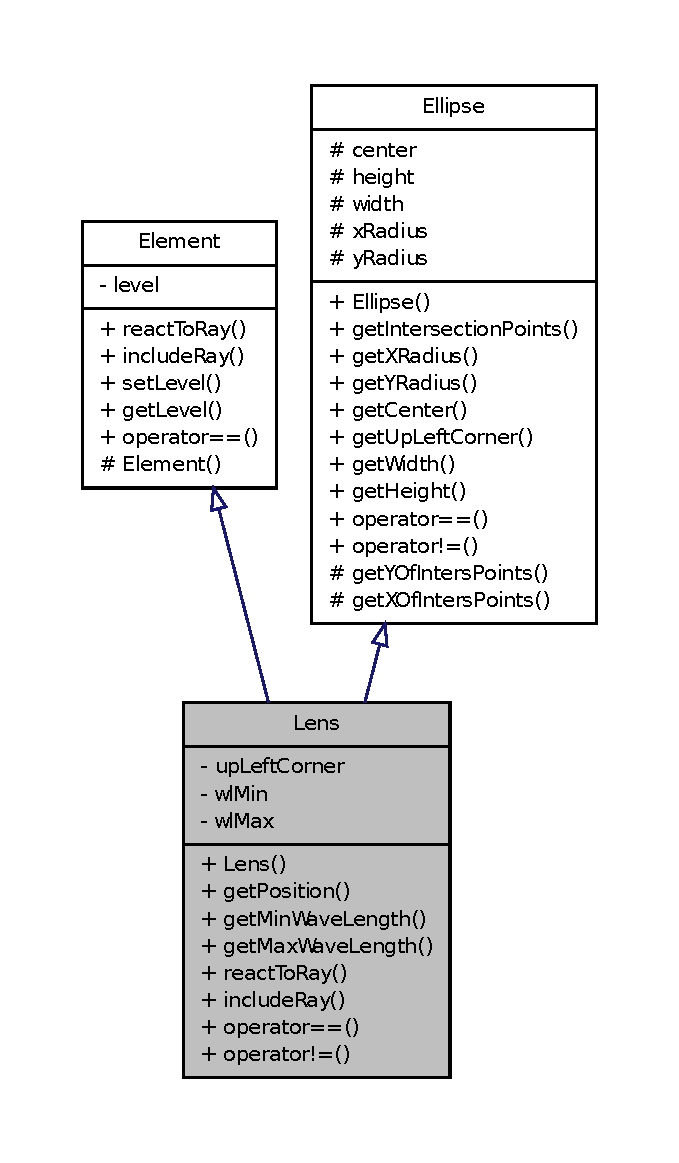
\includegraphics[height=550pt]{d4/def/classLens__inherit__graph}
\end{center}
\end{figure}


Graphe de collaboration de Lens\+:\nopagebreak
\begin{figure}[H]
\begin{center}
\leavevmode
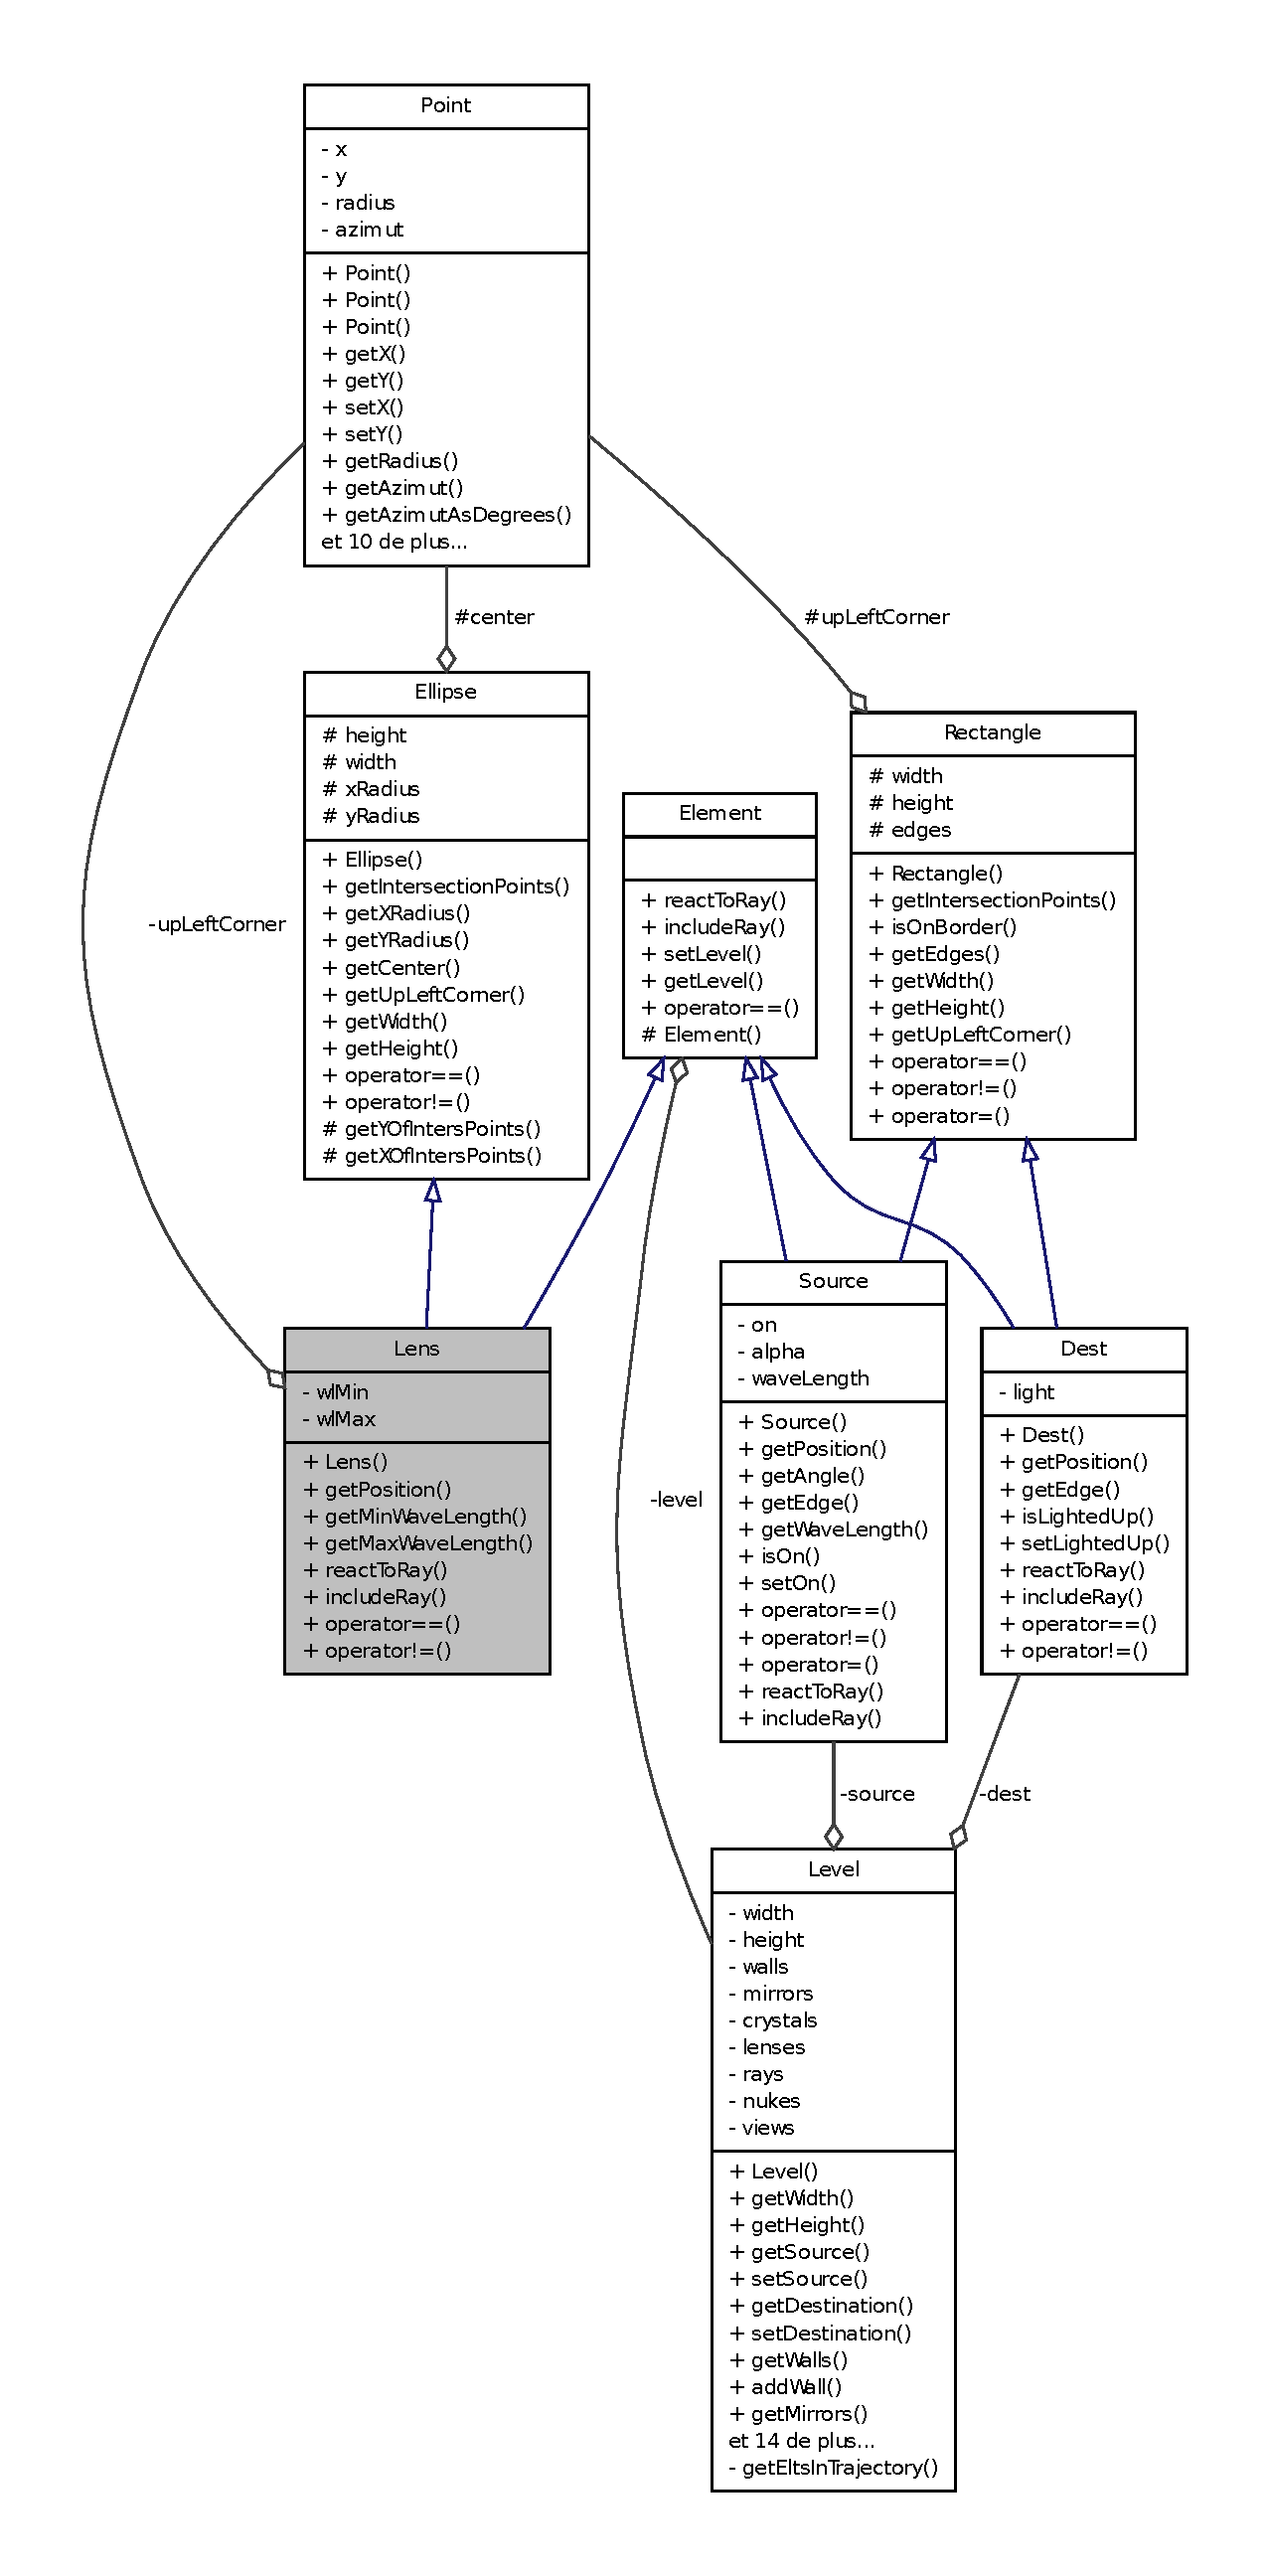
\includegraphics[height=550pt]{d8/df0/classLens__coll__graph}
\end{center}
\end{figure}


\subsection{Documentation des constructeurs et destructeur}
\hypertarget{classLens_a6dbd2d608178b9a15814f18d6dfb71d4}{}\index{Lens@{Lens}!Lens@{Lens}}
\index{Lens@{Lens}!Lens@{Lens}}
\subsubsection[{Lens(const Point \&, const int, const int, const int, const int)}]{\setlength{\rightskip}{0pt plus 5cm}Lens\+::\+Lens (
\begin{DoxyParamCaption}
\item[{const {\bf Point} \&}]{, }
\item[{const int}]{, }
\item[{const int}]{, }
\item[{const int}]{, }
\item[{const int}]{}
\end{DoxyParamCaption}
)}\label{classLens_a6dbd2d608178b9a15814f18d6dfb71d4}


Créer une nouvelle lentille pouvant être un obstacle à un rayon \+: si le rayon souhaite passer au travers, il devra être d\textquotesingle{}une longueur d\textquotesingle{}onde comprise dans l\textquotesingle{}intervalle souhaité par cette lentille. 

Dans le cas contraire, le rayon ne passera pas.


\begin{DoxyParams}{Paramètres}
{\em position} & La position du coin supérieur gauche du rectangle circonscrit à l\textquotesingle{}ellipse modélisant la lentille. \\
\hline
{\em width} & La largeur du rectangle circonscrit à la lentille. \\
\hline
{\em height} & la hauteur du rectangle circonscrit à la lentille. \\
\hline
{\em wl\+Min} & La longueur d\textquotesingle{}onde minimale des rayons autorisés à franchir la lentille. \\
\hline
{\em wl\+Max} & La longueur d\textquotesingle{}onde maximale des rayons autorisés à franchir la lentille. \\
\hline
\end{DoxyParams}


\subsection{Documentation des fonctions membres}
\hypertarget{classLens_ab042680cd439e4841b5c4358d4fad7a3}{}\index{Lens@{Lens}!get\+Max\+Wave\+Length@{get\+Max\+Wave\+Length}}
\index{get\+Max\+Wave\+Length@{get\+Max\+Wave\+Length}!Lens@{Lens}}
\subsubsection[{get\+Max\+Wave\+Length() const }]{\setlength{\rightskip}{0pt plus 5cm}int Lens\+::get\+Max\+Wave\+Length (
\begin{DoxyParamCaption}
{}
\end{DoxyParamCaption}
) const\hspace{0.3cm}{\ttfamily [inline]}}\label{classLens_ab042680cd439e4841b5c4358d4fad7a3}


Retourne la longueur d\textquotesingle{}onde maximale des rayons autorisés à franchir la lentille. 

\begin{DoxyReturn}{Renvoie}
La longueur d\textquotesingle{}onde maximale des rayon autorisés à franchir la lentille. 
\end{DoxyReturn}


Définition à la ligne 141 du fichier lens.\+hpp.



Références wl\+Max.


\begin{DoxyCode}
142 \{
143     \textcolor{keywordflow}{return} this->\hyperlink{classLens_ab9f83510445552c07c9b4b760ad92dd6}{wlMax};
144 \}
\end{DoxyCode}
\hypertarget{classLens_a14b3ba46e7f45c4850bc02b9f134cdbf}{}\index{Lens@{Lens}!get\+Min\+Wave\+Length@{get\+Min\+Wave\+Length}}
\index{get\+Min\+Wave\+Length@{get\+Min\+Wave\+Length}!Lens@{Lens}}
\subsubsection[{get\+Min\+Wave\+Length() const }]{\setlength{\rightskip}{0pt plus 5cm}int Lens\+::get\+Min\+Wave\+Length (
\begin{DoxyParamCaption}
{}
\end{DoxyParamCaption}
) const\hspace{0.3cm}{\ttfamily [inline]}}\label{classLens_a14b3ba46e7f45c4850bc02b9f134cdbf}


Retourne la longueur d\textquotesingle{}onde minimale des rayons autorisés à franchir la lentille. 

\begin{DoxyReturn}{Renvoie}
La longueur d\textquotesingle{}onde minimale des rayons autorisés à franchir la lentille. 
\end{DoxyReturn}


Définition à la ligne 136 du fichier lens.\+hpp.



Références wl\+Min.


\begin{DoxyCode}
137 \{
138     \textcolor{keywordflow}{return} this->\hyperlink{classLens_a14bcb2705ae2c2b120a642f0d44c75e2}{wlMin};
139 \}
\end{DoxyCode}
\hypertarget{classLens_a1eba530b7fd697dc651b59d6cbb077f1}{}\index{Lens@{Lens}!get\+Position@{get\+Position}}
\index{get\+Position@{get\+Position}!Lens@{Lens}}
\subsubsection[{get\+Position() const }]{\setlength{\rightskip}{0pt plus 5cm}const {\bf Point} \& Lens\+::get\+Position (
\begin{DoxyParamCaption}
{}
\end{DoxyParamCaption}
) const\hspace{0.3cm}{\ttfamily [inline]}}\label{classLens_a1eba530b7fd697dc651b59d6cbb077f1}


Retourne la position du coin supérieur gauche du rectangle circonscrit à la lentille. 

\begin{DoxyReturn}{Renvoie}
La coordonnée cartésienne du coin supérieur gauche du rectangle modélisant la lentille. 
\end{DoxyReturn}


Définition à la ligne 131 du fichier lens.\+hpp.



Références up\+Left\+Corner.


\begin{DoxyCode}
132 \{
133     \textcolor{keywordflow}{return} this->\hyperlink{classLens_af123a98958acdfca4cef5629ebfbbf4b}{upLeftCorner};
134 \}
\end{DoxyCode}
\hypertarget{classLens_a458286d40d04792b7a6db47bd9f775fc}{}\index{Lens@{Lens}!include\+Ray@{include\+Ray}}
\index{include\+Ray@{include\+Ray}!Lens@{Lens}}
\subsubsection[{include\+Ray(const Ray \&) const }]{\setlength{\rightskip}{0pt plus 5cm}{\bf Point}$\ast$ Lens\+::include\+Ray (
\begin{DoxyParamCaption}
\item[{const {\bf Ray} \&}]{}
\end{DoxyParamCaption}
) const\hspace{0.3cm}{\ttfamily [virtual]}}\label{classLens_a458286d40d04792b7a6db47bd9f775fc}


Renseigne si la lentille est dans la trajectoire du rayon. 


\begin{DoxyParams}{Paramètres}
{\em ray} & Le rayon.\\
\hline
\end{DoxyParams}
\begin{DoxyReturn}{Renvoie}
{\ttfamily true} Si la lentille se trouve dans la trajectoire du rayon entré en paramètre. 
\end{DoxyReturn}


Implémente \hyperlink{classElement_a1b88519623a6250155f7182706665448}{Element}.

\hypertarget{classLens_a78a86a6d5ec110881e9b876e3b13cea9}{}\index{Lens@{Lens}!operator"!=@{operator"!=}}
\index{operator"!=@{operator"!=}!Lens@{Lens}}
\subsubsection[{operator"!=(const Lens \&) const }]{\setlength{\rightskip}{0pt plus 5cm}bool Lens\+::operator!= (
\begin{DoxyParamCaption}
\item[{const {\bf Lens} \&}]{}
\end{DoxyParamCaption}
) const}\label{classLens_a78a86a6d5ec110881e9b876e3b13cea9}


Permet de savoir si deux lentilles sont différentes. 

\begin{DoxyReturn}{Renvoie}
{\ttfamily true} Si les deux lentilles sont différentes. 
\end{DoxyReturn}
\hypertarget{classLens_ad0f3fdc4b2b4945726994a4503f5252e}{}\index{Lens@{Lens}!operator==@{operator==}}
\index{operator==@{operator==}!Lens@{Lens}}
\subsubsection[{operator==(const Lens \&) const }]{\setlength{\rightskip}{0pt plus 5cm}bool Lens\+::operator== (
\begin{DoxyParamCaption}
\item[{const {\bf Lens} \&}]{}
\end{DoxyParamCaption}
) const}\label{classLens_ad0f3fdc4b2b4945726994a4503f5252e}


Permet de savoir si deux lentilles sont les mêmes. 

\begin{DoxyReturn}{Renvoie}
{\ttfamily true} Si les deux lentilles sont les même. 
\end{DoxyReturn}
\hypertarget{classLens_a3914a622c70a3c02f5f53fd33fa3340d}{}\index{Lens@{Lens}!react\+To\+Ray@{react\+To\+Ray}}
\index{react\+To\+Ray@{react\+To\+Ray}!Lens@{Lens}}
\subsubsection[{react\+To\+Ray(\+Ray)}]{\setlength{\rightskip}{0pt plus 5cm}void Lens\+::react\+To\+Ray (
\begin{DoxyParamCaption}
\item[{{\bf Ray}}]{}
\end{DoxyParamCaption}
)\hspace{0.3cm}{\ttfamily [virtual]}}\label{classLens_a3914a622c70a3c02f5f53fd33fa3340d}


Cette méthode est lancé lorsque la lentille courante est exposée à un rayon. 

Elle va communiquer au niveau la fin du rayon si il ne peut pas passer ou ne va rien faire si le rayon passe.


\begin{DoxyParams}{Paramètres}
{\em ray} & Un rayon percutant la lentille. \\
\hline
\end{DoxyParams}


Implémente \hyperlink{classElement_aa87116bb9422d64169b2ebf03831df9b}{Element}.



\subsection{Documentation des données membres}
\hypertarget{classLens_af123a98958acdfca4cef5629ebfbbf4b}{}\index{Lens@{Lens}!up\+Left\+Corner@{up\+Left\+Corner}}
\index{up\+Left\+Corner@{up\+Left\+Corner}!Lens@{Lens}}
\subsubsection[{up\+Left\+Corner}]{\setlength{\rightskip}{0pt plus 5cm}const {\bf Point} Lens\+::up\+Left\+Corner\hspace{0.3cm}{\ttfamily [private]}}\label{classLens_af123a98958acdfca4cef5629ebfbbf4b}


up\+Left\+Corner 



Définition à la ligne 30 du fichier lens.\+hpp.



Référencé par get\+Position().

\hypertarget{classLens_ab9f83510445552c07c9b4b760ad92dd6}{}\index{Lens@{Lens}!wl\+Max@{wl\+Max}}
\index{wl\+Max@{wl\+Max}!Lens@{Lens}}
\subsubsection[{wl\+Max}]{\setlength{\rightskip}{0pt plus 5cm}const int Lens\+::wl\+Max\hspace{0.3cm}{\ttfamily [private]}}\label{classLens_ab9f83510445552c07c9b4b760ad92dd6}


wl\+Max 



Définition à la ligne 40 du fichier lens.\+hpp.



Référencé par get\+Max\+Wave\+Length().

\hypertarget{classLens_a14bcb2705ae2c2b120a642f0d44c75e2}{}\index{Lens@{Lens}!wl\+Min@{wl\+Min}}
\index{wl\+Min@{wl\+Min}!Lens@{Lens}}
\subsubsection[{wl\+Min}]{\setlength{\rightskip}{0pt plus 5cm}const int Lens\+::wl\+Min\hspace{0.3cm}{\ttfamily [private]}}\label{classLens_a14bcb2705ae2c2b120a642f0d44c75e2}


wl\+Min 



Définition à la ligne 35 du fichier lens.\+hpp.



Référencé par get\+Min\+Wave\+Length().



La documentation de cette classe a été générée à partir du fichier suivant \+:\begin{DoxyCompactItemize}
\item 
model/elements/\hyperlink{lens_8hpp}{lens.\+hpp}\end{DoxyCompactItemize}

\hypertarget{classLevel}{}\section{Référence de la classe Level}
\label{classLevel}\index{Level@{Level}}


Modélise une carte telle qu\textquotesingle{}utilisée dans le jeu.  




{\ttfamily \#include $<$level.\+hpp$>$}

\subsection*{Fonctions membres publiques}
\begin{DoxyCompactItemize}
\item 
\hyperlink{classLevel_a97d9e4768c6b180d053a061fc99e66d1}{Level} (const double, const double)
\begin{DoxyCompactList}\small\item\em Instancie une carte de largeur et hauteur donnée. \end{DoxyCompactList}\item 
int \hyperlink{classLevel_a11ca1be00c88ed5c14774cf938509e61}{get\+Width} () const 
\begin{DoxyCompactList}\small\item\em Permet d\textquotesingle{}obtenir la longueur du niveau. \end{DoxyCompactList}\item 
int \hyperlink{classLevel_a0f867d54960aac1ceaa3b42fc7522924}{get\+Height} () const 
\begin{DoxyCompactList}\small\item\em Permet d\textquotesingle{}obtenir la hauteur du niveau. \end{DoxyCompactList}\item 
\hyperlink{classSource}{Source} \& \hyperlink{classLevel_a540f5c42d181bb948cf5f2c701ca3c7c}{get\+Source} ()
\begin{DoxyCompactList}\small\item\em Retourne la source de la carte. \end{DoxyCompactList}\item 
void \hyperlink{classLevel_ac867c06f1d2d3a7e5cf8ec59dd507c11}{set\+Source} (const \hyperlink{classSource}{Source} \&)
\begin{DoxyCompactList}\small\item\em Change la source de la carte. \end{DoxyCompactList}\item 
const \hyperlink{classDest}{Dest} \& \hyperlink{classLevel_aa545dc3931402ed464c7845386c45cbd}{get\+Destination} () const 
\begin{DoxyCompactList}\small\item\em Retourne la destination de la carte. \end{DoxyCompactList}\item 
void \hyperlink{classLevel_a6055c006cb8953d320cfb8974f066755}{set\+Destination} (const \hyperlink{classDest}{Dest} \&)
\begin{DoxyCompactList}\small\item\em Change la destination de la carte. \end{DoxyCompactList}\item 
const std\+::vector$<$ \hyperlink{classWall}{Wall} $>$ \& \hyperlink{classLevel_a5e80b38b27dba47b8f4f2b52accb76bc}{get\+Walls} () const 
\begin{DoxyCompactList}\small\item\em Retourne l\textquotesingle{}ensemble des murs de la carte. \end{DoxyCompactList}\item 
void \hyperlink{classLevel_ab72f4a67155fd0c16894a016a7bb767d}{add\+Wall} (const \hyperlink{classWall}{Wall} \&)
\begin{DoxyCompactList}\small\item\em Permet d\textquotesingle{}ajouter un mur sur la carte. \end{DoxyCompactList}\item 
std\+::vector$<$ \hyperlink{classMirror}{Mirror} $>$ \& \hyperlink{classLevel_a1c834cc0f3d69893d79f60de64d0d79a}{get\+Mirrors} ()
\begin{DoxyCompactList}\small\item\em Retourne l\textquotesingle{}ensemble des miroirs de la carte. \end{DoxyCompactList}\item 
void \hyperlink{classLevel_a9cc738973370d106ac629aacc4acea12}{add\+Mirror} (\hyperlink{classMirror}{Mirror})
\begin{DoxyCompactList}\small\item\em Permet d\textquotesingle{}ajouter un miroir sur la carte. \end{DoxyCompactList}\item 
const std\+::vector$<$ \hyperlink{classCrystal}{Crystal} $>$ \& \hyperlink{classLevel_aa36d324f88e7754b998499bafd5be068}{get\+Crystals} () const 
\begin{DoxyCompactList}\small\item\em Retourne l\textquotesingle{}ensemble des cristaux de la carte. \end{DoxyCompactList}\item 
void \hyperlink{classLevel_a2effcce70c0492609a9ecc403abcff70}{add\+Crystal} (\hyperlink{classCrystal}{Crystal})
\begin{DoxyCompactList}\small\item\em Permet d\textquotesingle{}ajouter un cristal sur la carte. \end{DoxyCompactList}\item 
const std\+::vector$<$ \hyperlink{classLens}{Lens} $>$ \& \hyperlink{classLevel_a9e8fa9a3da391138768af00f00e6c77b}{get\+Lenses} () const 
\begin{DoxyCompactList}\small\item\em Retourne l\textquotesingle{}ensemble des lentilles de la carte. \end{DoxyCompactList}\item 
void \hyperlink{classLevel_ae09f20a51cd8cb01244101f7ea7a1cef}{add\+Lens} (\hyperlink{classLens}{Lens})
\begin{DoxyCompactList}\small\item\em Permet d\textquotesingle{}ajouter une lentille sur la carte. \end{DoxyCompactList}\item 
std\+::vector$<$ \hyperlink{classRay}{Ray} $>$ \& \hyperlink{classLevel_ad2fa2a31db061681a3f237c80c348b46}{get\+Rays} ()
\begin{DoxyCompactList}\small\item\em Retourne l\textquotesingle{}ensemble des rayons de la carte. \end{DoxyCompactList}\item 
void \hyperlink{classLevel_a6528bd0b23a291644f7cb4278101af70}{set\+Rays} (const std\+::vector$<$ \hyperlink{classRay}{Ray} $>$ \&)
\begin{DoxyCompactList}\small\item\em Change l\textquotesingle{}ensemble des rayons de la carte. \end{DoxyCompactList}\item 
const std\+::vector$<$ \hyperlink{classNuke}{Nuke} $>$ \& \hyperlink{classLevel_ac1a78a1e0071ab24698705257cf82260}{get\+Nukes} () const 
\begin{DoxyCompactList}\small\item\em Retourne l\textquotesingle{}ensemble des bombes de la carte. \end{DoxyCompactList}\item 
void \hyperlink{classLevel_ac35e7ed887e6f823a08c987f17535e32}{add\+Nuke} (const \hyperlink{classNuke}{Nuke} \&)
\begin{DoxyCompactList}\small\item\em Permet d\textquotesingle{}ajouter une bombe sur la carte. \end{DoxyCompactList}\item 
bool \hyperlink{classLevel_ab52b9848381f3426728cfae132ae3120}{there\+Is\+An\+Exploded\+Nuke} () const 
\begin{DoxyCompactList}\small\item\em Renseigne si une bombe a explosé. \end{DoxyCompactList}\item 
void \hyperlink{classLevel_a9a04d35fd8f72d786707596c2e0efa66}{compute\+Ray} (\hyperlink{classRay}{Ray})
\begin{DoxyCompactList}\small\item\em Permet de calculer un rayon à partir du rayon entré en paramètre. \end{DoxyCompactList}\item 
void \hyperlink{classLevel_ad28d918ed43c60e845b8805cf9b6b139}{compute\+Rays} ()
\begin{DoxyCompactList}\small\item\em Calcule les rayons lumineux de la carte. \end{DoxyCompactList}\item 
void \hyperlink{classLevel_ae257142a2bb23b42a747ed7e6df520a4}{add\+View} (\hyperlink{classLevelView}{Level\+View} $\ast$)
\begin{DoxyCompactList}\small\item\em Permet d\textquotesingle{}abonner une nouvelle vue au modèle. \end{DoxyCompactList}\item 
void \hyperlink{classLevel_a9a4438ddbb8132978c4973618b366048}{notify\+Views} ()
\begin{DoxyCompactList}\small\item\em Permet de notifier les vues abonnées au niveau que son état a changé. \end{DoxyCompactList}\end{DoxyCompactItemize}
\subsection*{Fonctions membres privées}
\begin{DoxyCompactItemize}
\item 
std\+::map$<$ \hyperlink{classPoint}{Point} $\ast$, \hyperlink{classElement}{Element} $\ast$ $>$ \hyperlink{classLevel_a04fdb57c83687ebb4f89c5c5e925e712}{get\+Elts\+In\+Trajectory} (const \hyperlink{classRay}{Ray} \&ray)
\begin{DoxyCompactList}\small\item\em Permet d\textquotesingle{}obtenir une map contenant les élément se trouvant sur la trajectoire du rayon, ayant pour clé; le point d\textquotesingle{}intersection avec cet élément. \end{DoxyCompactList}\end{DoxyCompactItemize}
\subsection*{Attributs privés}
\begin{DoxyCompactItemize}
\item 
const double \hyperlink{classLevel_ae8e8f0fd1ed923ab9faf37bebb961cdf}{width}
\begin{DoxyCompactList}\small\item\em La largeur du niveau. \end{DoxyCompactList}\item 
const double \hyperlink{classLevel_a65034a4fcaebb97c0a640600d1681ae9}{height}
\begin{DoxyCompactList}\small\item\em La hauteur du niveau. \end{DoxyCompactList}\item 
\hyperlink{classSource}{Source} \hyperlink{classLevel_ad0687b252a6b49e840a34ca5288ead55}{source} \{\hyperlink{classPoint}{Point}\{0, 0\}, 10, 30., 400\}
\begin{DoxyCompactList}\small\item\em La source du niveau. \end{DoxyCompactList}\item 
\hyperlink{classDest}{Dest} \hyperlink{classLevel_adf6fd04f684283f895ad23a4d730b680}{dest} \{\hyperlink{classPoint}{Point}\{0, 0\}, 5\}
\begin{DoxyCompactList}\small\item\em La destination du niveau. \end{DoxyCompactList}\item 
std\+::vector$<$ \hyperlink{classWall}{Wall} $>$ \hyperlink{classLevel_a6f8ce53f3e8c3a2aadbfe1385c136d5a}{walls}
\begin{DoxyCompactList}\small\item\em L\textquotesingle{}ensemble des murs du niveau, qu\textquotesingle{}ils soient ceux qui le délimitent ou des murs supplémentaires ajoutés au niveau même. \end{DoxyCompactList}\item 
std\+::vector$<$ \hyperlink{classMirror}{Mirror} $>$ \hyperlink{classLevel_acdc507d55f78548739af4988d2af3647}{mirrors}
\begin{DoxyCompactList}\small\item\em mirrors L\textquotesingle{}ensemble des miroirs présents dans le niveau. \end{DoxyCompactList}\item 
std\+::vector$<$ \hyperlink{classCrystal}{Crystal} $>$ \hyperlink{classLevel_a68f233822a00e4ed880ddb180230ff3b}{crystals}
\begin{DoxyCompactList}\small\item\em crystals L\textquotesingle{}ensemble des cristaux présents dans le niveau. \end{DoxyCompactList}\item 
std\+::vector$<$ \hyperlink{classLens}{Lens} $>$ \hyperlink{classLevel_aaeb7900ce3b81586203e8746a47ab3e2}{lenses}
\begin{DoxyCompactList}\small\item\em lenses L\textquotesingle{}ensemble des lentilles présentes dans le niveau. \end{DoxyCompactList}\item 
std\+::vector$<$ \hyperlink{classRay}{Ray} $>$ \hyperlink{classLevel_a316fd189c069c2645f07be3862dc2caf}{rays}
\begin{DoxyCompactList}\small\item\em rays L\textquotesingle{}ensemble des rayons créés dans le niveau quand la source est allumée. \end{DoxyCompactList}\item 
std\+::vector$<$ \hyperlink{classNuke}{Nuke} $>$ \hyperlink{classLevel_a5fece1ffe87935a190ed156456ce410b}{nukes}
\begin{DoxyCompactList}\small\item\em nukes L\textquotesingle{}ensemble des bombes créées dans le niveau. \end{DoxyCompactList}\item 
std\+::vector$<$ \hyperlink{classLevelView}{Level\+View} $\ast$ $>$ \hyperlink{classLevel_a8a01947614ab3998f4c152882c113feb}{views}
\begin{DoxyCompactList}\small\item\em views L\textquotesingle{}ensemble des vues qui observent le niveau. \end{DoxyCompactList}\end{DoxyCompactItemize}


\subsection{Description détaillée}
Modélise une carte telle qu\textquotesingle{}utilisée dans le jeu. 

Une carte est un ensemble de composant tels que des murs, des miroirs, etc. 

Définition à la ligne 27 du fichier level.\+hpp.



Graphe de collaboration de Level\+:\nopagebreak
\begin{figure}[H]
\begin{center}
\leavevmode
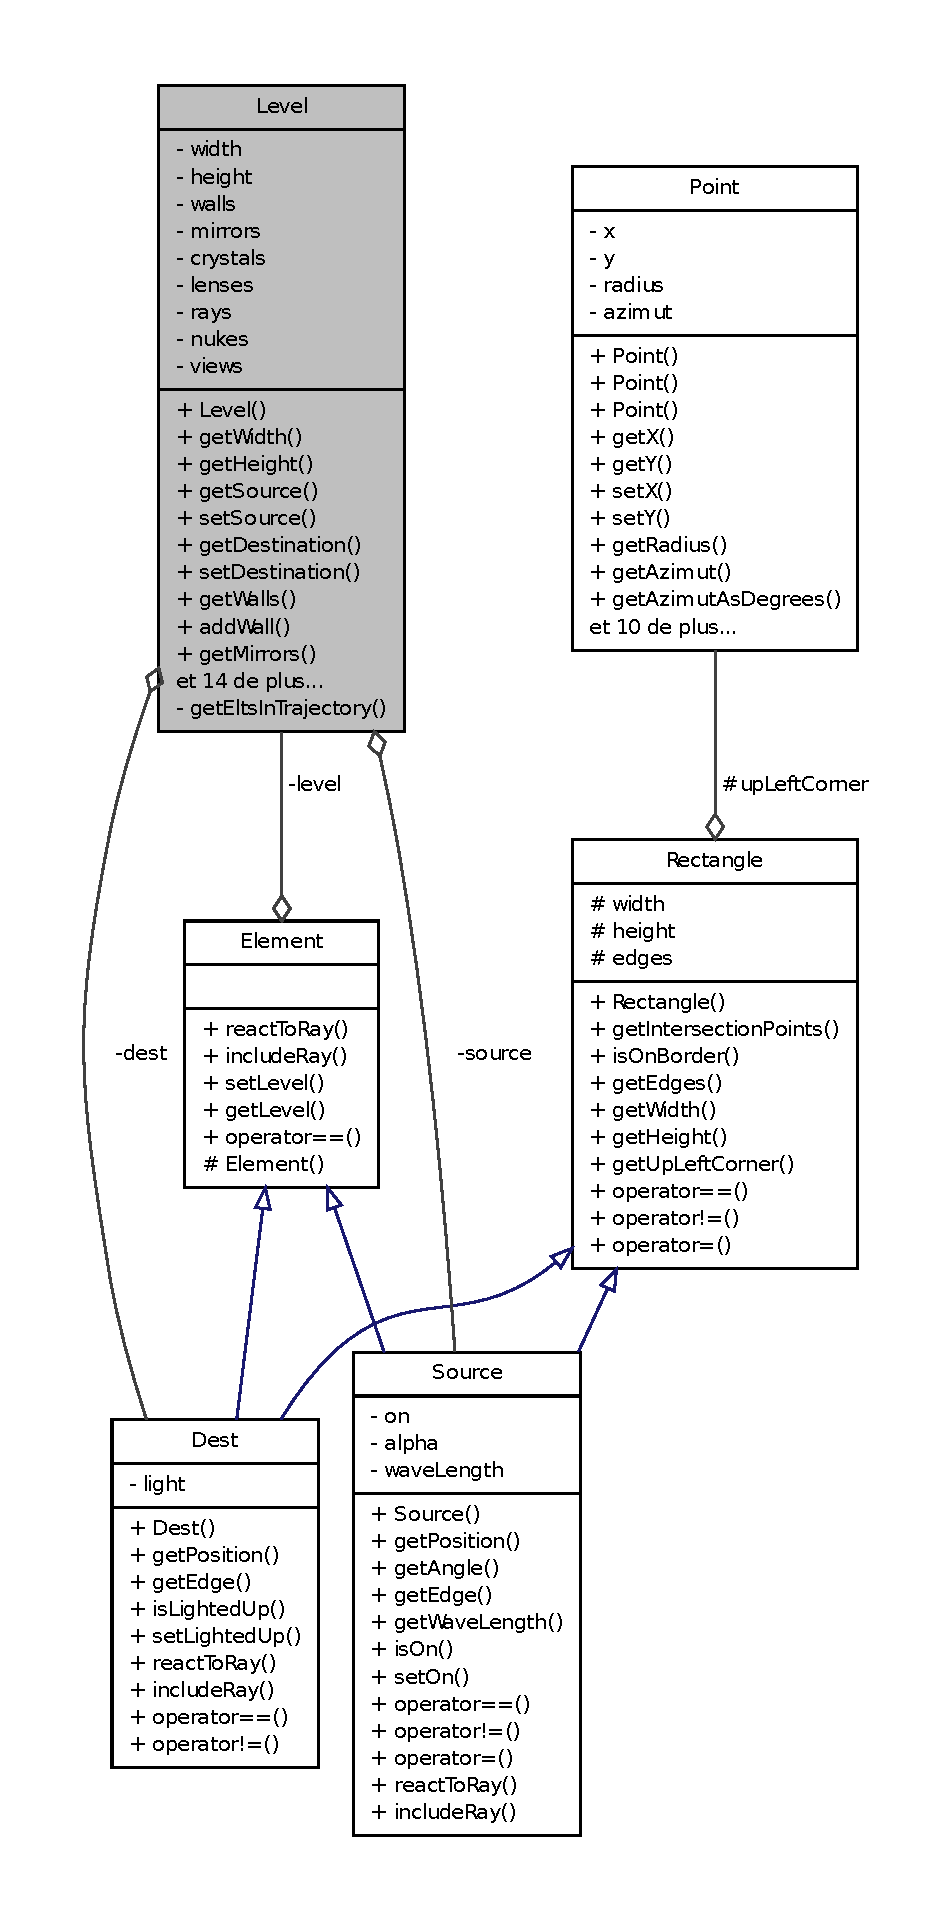
\includegraphics[height=550pt]{df/dee/classLevel__coll__graph}
\end{center}
\end{figure}


\subsection{Documentation des constructeurs et destructeur}
\hypertarget{classLevel_a97d9e4768c6b180d053a061fc99e66d1}{}\index{Level@{Level}!Level@{Level}}
\index{Level@{Level}!Level@{Level}}
\subsubsection[{Level(const double, const double)}]{\setlength{\rightskip}{0pt plus 5cm}Level\+::\+Level (
\begin{DoxyParamCaption}
\item[{const double}]{, }
\item[{const double}]{}
\end{DoxyParamCaption}
)}\label{classLevel_a97d9e4768c6b180d053a061fc99e66d1}


Instancie une carte de largeur et hauteur donnée. 

Quand une carte est crée, quatre murs dénotant ses bords sont automatiquement ajoutés à la carte. 

La source et la destination sont initialisées à des valeurs par défaut inutilisables. Vous devez manuellement initialiser la source et la destination via les fonctions appropriées. 
\begin{DoxyParams}{Paramètres}
{\em w} & la largeur de la carte \\
\hline
{\em h} & la hauteur de la carte \\
\hline
\end{DoxyParams}


\subsection{Documentation des fonctions membres}
\hypertarget{classLevel_a2effcce70c0492609a9ecc403abcff70}{}\index{Level@{Level}!add\+Crystal@{add\+Crystal}}
\index{add\+Crystal@{add\+Crystal}!Level@{Level}}
\subsubsection[{add\+Crystal(\+Crystal)}]{\setlength{\rightskip}{0pt plus 5cm}void Level\+::add\+Crystal (
\begin{DoxyParamCaption}
\item[{{\bf Crystal}}]{}
\end{DoxyParamCaption}
)}\label{classLevel_a2effcce70c0492609a9ecc403abcff70}


Permet d\textquotesingle{}ajouter un cristal sur la carte. 


\begin{DoxyParams}{Paramètres}
{\em new\+Crystal} & nouveau cristal à ajouter. \\
\hline
\end{DoxyParams}
\hypertarget{classLevel_ae09f20a51cd8cb01244101f7ea7a1cef}{}\index{Level@{Level}!add\+Lens@{add\+Lens}}
\index{add\+Lens@{add\+Lens}!Level@{Level}}
\subsubsection[{add\+Lens(\+Lens)}]{\setlength{\rightskip}{0pt plus 5cm}void Level\+::add\+Lens (
\begin{DoxyParamCaption}
\item[{{\bf Lens}}]{}
\end{DoxyParamCaption}
)}\label{classLevel_ae09f20a51cd8cb01244101f7ea7a1cef}


Permet d\textquotesingle{}ajouter une lentille sur la carte. 


\begin{DoxyParams}{Paramètres}
{\em new\+Lens} & nouvelle lentille à ajouter. \\
\hline
\end{DoxyParams}
\hypertarget{classLevel_a9cc738973370d106ac629aacc4acea12}{}\index{Level@{Level}!add\+Mirror@{add\+Mirror}}
\index{add\+Mirror@{add\+Mirror}!Level@{Level}}
\subsubsection[{add\+Mirror(\+Mirror)}]{\setlength{\rightskip}{0pt plus 5cm}void Level\+::add\+Mirror (
\begin{DoxyParamCaption}
\item[{{\bf Mirror}}]{}
\end{DoxyParamCaption}
)}\label{classLevel_a9cc738973370d106ac629aacc4acea12}


Permet d\textquotesingle{}ajouter un miroir sur la carte. 


\begin{DoxyParams}{Paramètres}
{\em new\+Mirror} & nouveau miroir à ajouter. \\
\hline
\end{DoxyParams}
\hypertarget{classLevel_ac35e7ed887e6f823a08c987f17535e32}{}\index{Level@{Level}!add\+Nuke@{add\+Nuke}}
\index{add\+Nuke@{add\+Nuke}!Level@{Level}}
\subsubsection[{add\+Nuke(const Nuke \&)}]{\setlength{\rightskip}{0pt plus 5cm}void Level\+::add\+Nuke (
\begin{DoxyParamCaption}
\item[{const {\bf Nuke} \&}]{}
\end{DoxyParamCaption}
)}\label{classLevel_ac35e7ed887e6f823a08c987f17535e32}


Permet d\textquotesingle{}ajouter une bombe sur la carte. 


\begin{DoxyParams}{Paramètres}
{\em new\+Nuke} & nouvelle bombe à ajouter. \\
\hline
\end{DoxyParams}
\hypertarget{classLevel_ae257142a2bb23b42a747ed7e6df520a4}{}\index{Level@{Level}!add\+View@{add\+View}}
\index{add\+View@{add\+View}!Level@{Level}}
\subsubsection[{add\+View(\+Level\+View $\ast$)}]{\setlength{\rightskip}{0pt plus 5cm}void Level\+::add\+View (
\begin{DoxyParamCaption}
\item[{{\bf Level\+View} $\ast$}]{}
\end{DoxyParamCaption}
)}\label{classLevel_ae257142a2bb23b42a747ed7e6df520a4}


Permet d\textquotesingle{}abonner une nouvelle vue au modèle. 


\begin{DoxyParams}{Paramètres}
{\em new\+View} & Nouvelle vue abonnée au niveau. \\
\hline
\end{DoxyParams}
\hypertarget{classLevel_ab72f4a67155fd0c16894a016a7bb767d}{}\index{Level@{Level}!add\+Wall@{add\+Wall}}
\index{add\+Wall@{add\+Wall}!Level@{Level}}
\subsubsection[{add\+Wall(const Wall \&)}]{\setlength{\rightskip}{0pt plus 5cm}void Level\+::add\+Wall (
\begin{DoxyParamCaption}
\item[{const {\bf Wall} \&}]{}
\end{DoxyParamCaption}
)}\label{classLevel_ab72f4a67155fd0c16894a016a7bb767d}


Permet d\textquotesingle{}ajouter un mur sur la carte. 


\begin{DoxyParams}{Paramètres}
{\em new\+Wall} & nouveau mur à ajouter. \\
\hline
\end{DoxyParams}
\hypertarget{classLevel_a9a04d35fd8f72d786707596c2e0efa66}{}\index{Level@{Level}!compute\+Ray@{compute\+Ray}}
\index{compute\+Ray@{compute\+Ray}!Level@{Level}}
\subsubsection[{compute\+Ray(\+Ray)}]{\setlength{\rightskip}{0pt plus 5cm}void Level\+::compute\+Ray (
\begin{DoxyParamCaption}
\item[{{\bf Ray}}]{}
\end{DoxyParamCaption}
)}\label{classLevel_a9a04d35fd8f72d786707596c2e0efa66}


Permet de calculer un rayon à partir du rayon entré en paramètre. 


\begin{DoxyParams}{Paramètres}
{\em ray} & Rayon précèdent. \\
\hline
\end{DoxyParams}
\hypertarget{classLevel_ad28d918ed43c60e845b8805cf9b6b139}{}\index{Level@{Level}!compute\+Rays@{compute\+Rays}}
\index{compute\+Rays@{compute\+Rays}!Level@{Level}}
\subsubsection[{compute\+Rays()}]{\setlength{\rightskip}{0pt plus 5cm}void Level\+::compute\+Rays (
\begin{DoxyParamCaption}
{}
\end{DoxyParamCaption}
)}\label{classLevel_ad28d918ed43c60e845b8805cf9b6b139}


Calcule les rayons lumineux de la carte. 

\hypertarget{classLevel_aa36d324f88e7754b998499bafd5be068}{}\index{Level@{Level}!get\+Crystals@{get\+Crystals}}
\index{get\+Crystals@{get\+Crystals}!Level@{Level}}
\subsubsection[{get\+Crystals() const }]{\setlength{\rightskip}{0pt plus 5cm}const std\+::vector$<$ {\bf Crystal} $>$ \& Level\+::get\+Crystals (
\begin{DoxyParamCaption}
{}
\end{DoxyParamCaption}
) const\hspace{0.3cm}{\ttfamily [inline]}}\label{classLevel_aa36d324f88e7754b998499bafd5be068}


Retourne l\textquotesingle{}ensemble des cristaux de la carte. 

\begin{DoxyReturn}{Renvoie}
l\textquotesingle{}ensemble des cristaux de la carte 
\end{DoxyReturn}


Définition à la ligne 308 du fichier level.\+hpp.



Références crystals.


\begin{DoxyCode}
309 \{
310     \textcolor{keywordflow}{return} this->\hyperlink{classLevel_a68f233822a00e4ed880ddb180230ff3b}{crystals};
311 \}
\end{DoxyCode}
\hypertarget{classLevel_aa545dc3931402ed464c7845386c45cbd}{}\index{Level@{Level}!get\+Destination@{get\+Destination}}
\index{get\+Destination@{get\+Destination}!Level@{Level}}
\subsubsection[{get\+Destination() const }]{\setlength{\rightskip}{0pt plus 5cm}const {\bf Dest} \& Level\+::get\+Destination (
\begin{DoxyParamCaption}
{}
\end{DoxyParamCaption}
) const\hspace{0.3cm}{\ttfamily [inline]}}\label{classLevel_aa545dc3931402ed464c7845386c45cbd}


Retourne la destination de la carte. 

\begin{DoxyReturn}{Renvoie}
la destination de la carte 
\end{DoxyReturn}


Définition à la ligne 293 du fichier level.\+hpp.



Références dest.


\begin{DoxyCode}
294 \{
295     \textcolor{keywordflow}{return} this->\hyperlink{classLevel_adf6fd04f684283f895ad23a4d730b680}{dest};
296 \}
\end{DoxyCode}
\hypertarget{classLevel_a04fdb57c83687ebb4f89c5c5e925e712}{}\index{Level@{Level}!get\+Elts\+In\+Trajectory@{get\+Elts\+In\+Trajectory}}
\index{get\+Elts\+In\+Trajectory@{get\+Elts\+In\+Trajectory}!Level@{Level}}
\subsubsection[{get\+Elts\+In\+Trajectory(const Ray \&ray)}]{\setlength{\rightskip}{0pt plus 5cm}std\+::map$<${\bf Point} $\ast$, {\bf Element} $\ast$$>$ Level\+::get\+Elts\+In\+Trajectory (
\begin{DoxyParamCaption}
\item[{const {\bf Ray} \&}]{ray}
\end{DoxyParamCaption}
)\hspace{0.3cm}{\ttfamily [private]}}\label{classLevel_a04fdb57c83687ebb4f89c5c5e925e712}


Permet d\textquotesingle{}obtenir une map contenant les élément se trouvant sur la trajectoire du rayon, ayant pour clé; le point d\textquotesingle{}intersection avec cet élément. 


\begin{DoxyParams}{Paramètres}
{\em ray} & Rayon dont on désire obtenir les éléments sur sa trajectoire.\\
\hline
\end{DoxyParams}
\begin{DoxyReturn}{Renvoie}
Une map contenant les élément se trouvant sur la trajectoire du rayon, ayant pour clé; le point d\textquotesingle{}intersection avec cet élément. 
\end{DoxyReturn}
\hypertarget{classLevel_a0f867d54960aac1ceaa3b42fc7522924}{}\index{Level@{Level}!get\+Height@{get\+Height}}
\index{get\+Height@{get\+Height}!Level@{Level}}
\subsubsection[{get\+Height() const }]{\setlength{\rightskip}{0pt plus 5cm}int Level\+::get\+Height (
\begin{DoxyParamCaption}
{}
\end{DoxyParamCaption}
) const\hspace{0.3cm}{\ttfamily [inline]}}\label{classLevel_a0f867d54960aac1ceaa3b42fc7522924}


Permet d\textquotesingle{}obtenir la hauteur du niveau. 

\begin{DoxyReturn}{Renvoie}
la hauteur du niveau. 
\end{DoxyReturn}


Définition à la ligne 283 du fichier level.\+hpp.



Références height, et utilities\+::round().


\begin{DoxyCode}
284 \{
285     \textcolor{keywordflow}{return} \hyperlink{namespaceutilities_a00ae09dc5ce4274969a2a28607426eb5}{std::round}(this->\hyperlink{classLevel_a65034a4fcaebb97c0a640600d1681ae9}{height});
286 \}
\end{DoxyCode}
\hypertarget{classLevel_a9e8fa9a3da391138768af00f00e6c77b}{}\index{Level@{Level}!get\+Lenses@{get\+Lenses}}
\index{get\+Lenses@{get\+Lenses}!Level@{Level}}
\subsubsection[{get\+Lenses() const }]{\setlength{\rightskip}{0pt plus 5cm}const std\+::vector$<$ {\bf Lens} $>$ \& Level\+::get\+Lenses (
\begin{DoxyParamCaption}
{}
\end{DoxyParamCaption}
) const\hspace{0.3cm}{\ttfamily [inline]}}\label{classLevel_a9e8fa9a3da391138768af00f00e6c77b}


Retourne l\textquotesingle{}ensemble des lentilles de la carte. 

\begin{DoxyReturn}{Renvoie}
l\textquotesingle{}ensemble des lentilles de la carte 
\end{DoxyReturn}


Définition à la ligne 313 du fichier level.\+hpp.



Références lenses.


\begin{DoxyCode}
314 \{
315     \textcolor{keywordflow}{return} this->\hyperlink{classLevel_aaeb7900ce3b81586203e8746a47ab3e2}{lenses};
316 \}
\end{DoxyCode}
\hypertarget{classLevel_a1c834cc0f3d69893d79f60de64d0d79a}{}\index{Level@{Level}!get\+Mirrors@{get\+Mirrors}}
\index{get\+Mirrors@{get\+Mirrors}!Level@{Level}}
\subsubsection[{get\+Mirrors()}]{\setlength{\rightskip}{0pt plus 5cm}std\+::vector$<$ {\bf Mirror} $>$ \& Level\+::get\+Mirrors (
\begin{DoxyParamCaption}
{}
\end{DoxyParamCaption}
)\hspace{0.3cm}{\ttfamily [inline]}}\label{classLevel_a1c834cc0f3d69893d79f60de64d0d79a}


Retourne l\textquotesingle{}ensemble des miroirs de la carte. 

\begin{DoxyReturn}{Renvoie}
l\textquotesingle{}ensemble des miroirs de la carte 
\end{DoxyReturn}


Définition à la ligne 303 du fichier level.\+hpp.



Références mirrors.


\begin{DoxyCode}
304 \{
305     \textcolor{keywordflow}{return} this->\hyperlink{classLevel_acdc507d55f78548739af4988d2af3647}{mirrors};
306 \}
\end{DoxyCode}
\hypertarget{classLevel_ac1a78a1e0071ab24698705257cf82260}{}\index{Level@{Level}!get\+Nukes@{get\+Nukes}}
\index{get\+Nukes@{get\+Nukes}!Level@{Level}}
\subsubsection[{get\+Nukes() const }]{\setlength{\rightskip}{0pt plus 5cm}const std\+::vector$<$ {\bf Nuke} $>$ \& Level\+::get\+Nukes (
\begin{DoxyParamCaption}
{}
\end{DoxyParamCaption}
) const\hspace{0.3cm}{\ttfamily [inline]}}\label{classLevel_ac1a78a1e0071ab24698705257cf82260}


Retourne l\textquotesingle{}ensemble des bombes de la carte. 

\begin{DoxyReturn}{Renvoie}
l\textquotesingle{}ensemble des bombes de la carte 
\end{DoxyReturn}


Définition à la ligne 323 du fichier level.\+hpp.



Références nukes.


\begin{DoxyCode}
324 \{
325     \textcolor{keywordflow}{return} this->\hyperlink{classLevel_a5fece1ffe87935a190ed156456ce410b}{nukes};
326 \}
\end{DoxyCode}
\hypertarget{classLevel_ad2fa2a31db061681a3f237c80c348b46}{}\index{Level@{Level}!get\+Rays@{get\+Rays}}
\index{get\+Rays@{get\+Rays}!Level@{Level}}
\subsubsection[{get\+Rays()}]{\setlength{\rightskip}{0pt plus 5cm}std\+::vector$<$ {\bf Ray} $>$ \& Level\+::get\+Rays (
\begin{DoxyParamCaption}
{}
\end{DoxyParamCaption}
)\hspace{0.3cm}{\ttfamily [inline]}}\label{classLevel_ad2fa2a31db061681a3f237c80c348b46}


Retourne l\textquotesingle{}ensemble des rayons de la carte. 

\begin{DoxyReturn}{Renvoie}
l\textquotesingle{}ensemble des rayons de la carte 
\end{DoxyReturn}


Définition à la ligne 318 du fichier level.\+hpp.



Références rays.


\begin{DoxyCode}
319 \{
320     \textcolor{keywordflow}{return} this->\hyperlink{classLevel_a316fd189c069c2645f07be3862dc2caf}{rays};
321 \}
\end{DoxyCode}
\hypertarget{classLevel_a540f5c42d181bb948cf5f2c701ca3c7c}{}\index{Level@{Level}!get\+Source@{get\+Source}}
\index{get\+Source@{get\+Source}!Level@{Level}}
\subsubsection[{get\+Source()}]{\setlength{\rightskip}{0pt plus 5cm}{\bf Source} \& Level\+::get\+Source (
\begin{DoxyParamCaption}
{}
\end{DoxyParamCaption}
)\hspace{0.3cm}{\ttfamily [inline]}}\label{classLevel_a540f5c42d181bb948cf5f2c701ca3c7c}


Retourne la source de la carte. 

\begin{DoxyReturn}{Renvoie}
la source de la carte. 
\end{DoxyReturn}


Définition à la ligne 288 du fichier level.\+hpp.



Références source.


\begin{DoxyCode}
289 \{
290     \textcolor{keywordflow}{return} this->\hyperlink{classLevel_ad0687b252a6b49e840a34ca5288ead55}{source};
291 \}
\end{DoxyCode}
\hypertarget{classLevel_a5e80b38b27dba47b8f4f2b52accb76bc}{}\index{Level@{Level}!get\+Walls@{get\+Walls}}
\index{get\+Walls@{get\+Walls}!Level@{Level}}
\subsubsection[{get\+Walls() const }]{\setlength{\rightskip}{0pt plus 5cm}const std\+::vector$<$ {\bf Wall} $>$ \& Level\+::get\+Walls (
\begin{DoxyParamCaption}
{}
\end{DoxyParamCaption}
) const\hspace{0.3cm}{\ttfamily [inline]}}\label{classLevel_a5e80b38b27dba47b8f4f2b52accb76bc}


Retourne l\textquotesingle{}ensemble des murs de la carte. 

\begin{DoxyReturn}{Renvoie}
l\textquotesingle{}ensemble des murs de la carte 
\end{DoxyReturn}


Définition à la ligne 298 du fichier level.\+hpp.



Références walls.


\begin{DoxyCode}
299 \{
300     \textcolor{keywordflow}{return} this->\hyperlink{classLevel_a6f8ce53f3e8c3a2aadbfe1385c136d5a}{walls};
301 \}
\end{DoxyCode}
\hypertarget{classLevel_a11ca1be00c88ed5c14774cf938509e61}{}\index{Level@{Level}!get\+Width@{get\+Width}}
\index{get\+Width@{get\+Width}!Level@{Level}}
\subsubsection[{get\+Width() const }]{\setlength{\rightskip}{0pt plus 5cm}int Level\+::get\+Width (
\begin{DoxyParamCaption}
{}
\end{DoxyParamCaption}
) const\hspace{0.3cm}{\ttfamily [inline]}}\label{classLevel_a11ca1be00c88ed5c14774cf938509e61}


Permet d\textquotesingle{}obtenir la longueur du niveau. 

\begin{DoxyReturn}{Renvoie}
La longueur du niveau. 
\end{DoxyReturn}


Définition à la ligne 278 du fichier level.\+hpp.



Références utilities\+::round(), et width.


\begin{DoxyCode}
279 \{
280     \textcolor{keywordflow}{return} \hyperlink{namespaceutilities_a00ae09dc5ce4274969a2a28607426eb5}{std::round}(this->\hyperlink{classLevel_ae8e8f0fd1ed923ab9faf37bebb961cdf}{width});
281 \}
\end{DoxyCode}
\hypertarget{classLevel_a9a4438ddbb8132978c4973618b366048}{}\index{Level@{Level}!notify\+Views@{notify\+Views}}
\index{notify\+Views@{notify\+Views}!Level@{Level}}
\subsubsection[{notify\+Views()}]{\setlength{\rightskip}{0pt plus 5cm}void Level\+::notify\+Views (
\begin{DoxyParamCaption}
{}
\end{DoxyParamCaption}
)}\label{classLevel_a9a4438ddbb8132978c4973618b366048}


Permet de notifier les vues abonnées au niveau que son état a changé. 

\hypertarget{classLevel_a6055c006cb8953d320cfb8974f066755}{}\index{Level@{Level}!set\+Destination@{set\+Destination}}
\index{set\+Destination@{set\+Destination}!Level@{Level}}
\subsubsection[{set\+Destination(const Dest \&)}]{\setlength{\rightskip}{0pt plus 5cm}void Level\+::set\+Destination (
\begin{DoxyParamCaption}
\item[{const {\bf Dest} \&}]{}
\end{DoxyParamCaption}
)}\label{classLevel_a6055c006cb8953d320cfb8974f066755}


Change la destination de la carte. 


\begin{DoxyParams}{Paramètres}
{\em value} & la destination de la carte \\
\hline
\end{DoxyParams}
\hypertarget{classLevel_a6528bd0b23a291644f7cb4278101af70}{}\index{Level@{Level}!set\+Rays@{set\+Rays}}
\index{set\+Rays@{set\+Rays}!Level@{Level}}
\subsubsection[{set\+Rays(const std\+::vector$<$ Ray $>$ \&)}]{\setlength{\rightskip}{0pt plus 5cm}void Level\+::set\+Rays (
\begin{DoxyParamCaption}
\item[{const std\+::vector$<$ {\bf Ray} $>$ \&}]{}
\end{DoxyParamCaption}
)}\label{classLevel_a6528bd0b23a291644f7cb4278101af70}


Change l\textquotesingle{}ensemble des rayons de la carte. 


\begin{DoxyParams}{Paramètres}
{\em le} & nouvel ensemble de rayons de la carte \\
\hline
\end{DoxyParams}
\hypertarget{classLevel_ac867c06f1d2d3a7e5cf8ec59dd507c11}{}\index{Level@{Level}!set\+Source@{set\+Source}}
\index{set\+Source@{set\+Source}!Level@{Level}}
\subsubsection[{set\+Source(const Source \&)}]{\setlength{\rightskip}{0pt plus 5cm}void Level\+::set\+Source (
\begin{DoxyParamCaption}
\item[{const {\bf Source} \&}]{}
\end{DoxyParamCaption}
)}\label{classLevel_ac867c06f1d2d3a7e5cf8ec59dd507c11}


Change la source de la carte. 


\begin{DoxyParams}{Paramètres}
{\em value} & la nouvelle source \\
\hline
\end{DoxyParams}
\hypertarget{classLevel_ab52b9848381f3426728cfae132ae3120}{}\index{Level@{Level}!there\+Is\+An\+Exploded\+Nuke@{there\+Is\+An\+Exploded\+Nuke}}
\index{there\+Is\+An\+Exploded\+Nuke@{there\+Is\+An\+Exploded\+Nuke}!Level@{Level}}
\subsubsection[{there\+Is\+An\+Exploded\+Nuke() const }]{\setlength{\rightskip}{0pt plus 5cm}bool Level\+::there\+Is\+An\+Exploded\+Nuke (
\begin{DoxyParamCaption}
{}
\end{DoxyParamCaption}
) const}\label{classLevel_ab52b9848381f3426728cfae132ae3120}


Renseigne si une bombe a explosé. 

\begin{DoxyReturn}{Renvoie}
{\ttfamily true} Si une bombe a explosé. 
\end{DoxyReturn}


\subsection{Documentation des données membres}
\hypertarget{classLevel_a68f233822a00e4ed880ddb180230ff3b}{}\index{Level@{Level}!crystals@{crystals}}
\index{crystals@{crystals}!Level@{Level}}
\subsubsection[{crystals}]{\setlength{\rightskip}{0pt plus 5cm}std\+::vector$<${\bf Crystal}$>$ Level\+::crystals\hspace{0.3cm}{\ttfamily [private]}}\label{classLevel_a68f233822a00e4ed880ddb180230ff3b}


crystals L\textquotesingle{}ensemble des cristaux présents dans le niveau. 



Définition à la ligne 65 du fichier level.\+hpp.



Référencé par get\+Crystals().

\hypertarget{classLevel_adf6fd04f684283f895ad23a4d730b680}{}\index{Level@{Level}!dest@{dest}}
\index{dest@{dest}!Level@{Level}}
\subsubsection[{dest}]{\setlength{\rightskip}{0pt plus 5cm}{\bf Dest} Level\+::dest \{{\bf Point}\{0, 0\}, 5\}\hspace{0.3cm}{\ttfamily [private]}}\label{classLevel_adf6fd04f684283f895ad23a4d730b680}


La destination du niveau. 



Définition à la ligne 49 du fichier level.\+hpp.



Référencé par get\+Destination().

\hypertarget{classLevel_a65034a4fcaebb97c0a640600d1681ae9}{}\index{Level@{Level}!height@{height}}
\index{height@{height}!Level@{Level}}
\subsubsection[{height}]{\setlength{\rightskip}{0pt plus 5cm}const double Level\+::height\hspace{0.3cm}{\ttfamily [private]}}\label{classLevel_a65034a4fcaebb97c0a640600d1681ae9}


La hauteur du niveau. 



Définition à la ligne 39 du fichier level.\+hpp.



Référencé par get\+Height().

\hypertarget{classLevel_aaeb7900ce3b81586203e8746a47ab3e2}{}\index{Level@{Level}!lenses@{lenses}}
\index{lenses@{lenses}!Level@{Level}}
\subsubsection[{lenses}]{\setlength{\rightskip}{0pt plus 5cm}std\+::vector$<${\bf Lens}$>$ Level\+::lenses\hspace{0.3cm}{\ttfamily [private]}}\label{classLevel_aaeb7900ce3b81586203e8746a47ab3e2}


lenses L\textquotesingle{}ensemble des lentilles présentes dans le niveau. 



Définition à la ligne 70 du fichier level.\+hpp.



Référencé par get\+Lenses().

\hypertarget{classLevel_acdc507d55f78548739af4988d2af3647}{}\index{Level@{Level}!mirrors@{mirrors}}
\index{mirrors@{mirrors}!Level@{Level}}
\subsubsection[{mirrors}]{\setlength{\rightskip}{0pt plus 5cm}std\+::vector$<${\bf Mirror}$>$ Level\+::mirrors\hspace{0.3cm}{\ttfamily [private]}}\label{classLevel_acdc507d55f78548739af4988d2af3647}


mirrors L\textquotesingle{}ensemble des miroirs présents dans le niveau. 



Définition à la ligne 60 du fichier level.\+hpp.



Référencé par get\+Mirrors().

\hypertarget{classLevel_a5fece1ffe87935a190ed156456ce410b}{}\index{Level@{Level}!nukes@{nukes}}
\index{nukes@{nukes}!Level@{Level}}
\subsubsection[{nukes}]{\setlength{\rightskip}{0pt plus 5cm}std\+::vector$<${\bf Nuke}$>$ Level\+::nukes\hspace{0.3cm}{\ttfamily [private]}}\label{classLevel_a5fece1ffe87935a190ed156456ce410b}


nukes L\textquotesingle{}ensemble des bombes créées dans le niveau. 



Définition à la ligne 81 du fichier level.\+hpp.



Référencé par get\+Nukes().

\hypertarget{classLevel_a316fd189c069c2645f07be3862dc2caf}{}\index{Level@{Level}!rays@{rays}}
\index{rays@{rays}!Level@{Level}}
\subsubsection[{rays}]{\setlength{\rightskip}{0pt plus 5cm}std\+::vector$<${\bf Ray}$>$ Level\+::rays\hspace{0.3cm}{\ttfamily [private]}}\label{classLevel_a316fd189c069c2645f07be3862dc2caf}


rays L\textquotesingle{}ensemble des rayons créés dans le niveau quand la source est allumée. 



Définition à la ligne 76 du fichier level.\+hpp.



Référencé par get\+Rays().

\hypertarget{classLevel_ad0687b252a6b49e840a34ca5288ead55}{}\index{Level@{Level}!source@{source}}
\index{source@{source}!Level@{Level}}
\subsubsection[{source}]{\setlength{\rightskip}{0pt plus 5cm}{\bf Source} Level\+::source \{{\bf Point}\{0, 0\}, 10, 30., 400\}\hspace{0.3cm}{\ttfamily [private]}}\label{classLevel_ad0687b252a6b49e840a34ca5288ead55}


La source du niveau. 



Définition à la ligne 44 du fichier level.\+hpp.



Référencé par get\+Source().

\hypertarget{classLevel_a8a01947614ab3998f4c152882c113feb}{}\index{Level@{Level}!views@{views}}
\index{views@{views}!Level@{Level}}
\subsubsection[{views}]{\setlength{\rightskip}{0pt plus 5cm}std\+::vector$<${\bf Level\+View} $\ast$$>$ Level\+::views\hspace{0.3cm}{\ttfamily [private]}}\label{classLevel_a8a01947614ab3998f4c152882c113feb}


views L\textquotesingle{}ensemble des vues qui observent le niveau. 



Définition à la ligne 86 du fichier level.\+hpp.

\hypertarget{classLevel_a6f8ce53f3e8c3a2aadbfe1385c136d5a}{}\index{Level@{Level}!walls@{walls}}
\index{walls@{walls}!Level@{Level}}
\subsubsection[{walls}]{\setlength{\rightskip}{0pt plus 5cm}std\+::vector$<${\bf Wall}$>$ Level\+::walls\hspace{0.3cm}{\ttfamily [private]}}\label{classLevel_a6f8ce53f3e8c3a2aadbfe1385c136d5a}


L\textquotesingle{}ensemble des murs du niveau, qu\textquotesingle{}ils soient ceux qui le délimitent ou des murs supplémentaires ajoutés au niveau même. 



Définition à la ligne 55 du fichier level.\+hpp.



Référencé par get\+Walls().

\hypertarget{classLevel_ae8e8f0fd1ed923ab9faf37bebb961cdf}{}\index{Level@{Level}!width@{width}}
\index{width@{width}!Level@{Level}}
\subsubsection[{width}]{\setlength{\rightskip}{0pt plus 5cm}const double Level\+::width\hspace{0.3cm}{\ttfamily [private]}}\label{classLevel_ae8e8f0fd1ed923ab9faf37bebb961cdf}


La largeur du niveau. 



Définition à la ligne 34 du fichier level.\+hpp.



Référencé par get\+Width().



La documentation de cette classe a été générée à partir du fichier suivant \+:\begin{DoxyCompactItemize}
\item 
model/elements/\hyperlink{level_8hpp}{level.\+hpp}\end{DoxyCompactItemize}

\hypertarget{classLevelView}{}\section{Référence de la classe Level\+View}
\label{classLevelView}\index{Level\+View@{Level\+View}}


Cette classe représente le niveau qui va être joué lors d\textquotesingle{}une partie.  




{\ttfamily \#include $<$levelview.\+hpp$>$}

\subsection*{Connecteurs publics}
\begin{DoxyCompactItemize}
\item 
void \hyperlink{classLevelView_ae8298aa5d3163d7cc1343adbb2676d8a}{set\+Level\+File\+Path} (const Q\+String)
\begin{DoxyCompactList}\small\item\em Permet de changer le fichier de niveau et d\textquotesingle{}afficher ce niveau. \end{DoxyCompactList}\item 
void \hyperlink{classLevelView_a3bded54066b2ce49cf972b16d03817bb}{load\+Level\+From\+File} ()
\begin{DoxyCompactList}\small\item\em Permet d\textquotesingle{}afficher le fichier niveau dont la vue courante contient le chemin en attribut. \end{DoxyCompactList}\item 
void \hyperlink{classLevelView_a3ada0dd54a12cc91a31113dd83553f3a}{update\+Display} ()
\begin{DoxyCompactList}\small\item\em Permet de rafraichir l\textquotesingle{}affichage lorsque le niveau change d\textquotesingle{}état. \end{DoxyCompactList}\item 
void \hyperlink{classLevelView_ad6ea3472fed0f3aa469779b6efac3b41}{display\+End\+Of\+Game} ()
\begin{DoxyCompactList}\small\item\em Permet d\textquotesingle{}afficher une boite de dialogue informant l\textquotesingle{}utilisateur de la fin du jeu. \end{DoxyCompactList}\end{DoxyCompactItemize}
\subsection*{Signaux}
\begin{DoxyCompactItemize}
\item 
void \hyperlink{classLevelView_a3953bf386139bae926640e8c9e90b5fe}{displaying\+Started} ()
\begin{DoxyCompactList}\small\item\em Signale que le niveau doit être affiché. \end{DoxyCompactList}\item 
void \hyperlink{classLevelView_a4e35d1b0b0fa00a1a4c602da15471359}{displaying\+Stopped} ()
\begin{DoxyCompactList}\small\item\em Signale que le niveau ne doit plus être affiché. \end{DoxyCompactList}\end{DoxyCompactItemize}
\subsection*{Fonctions membres publiques}
\begin{DoxyCompactItemize}
\item 
\hyperlink{classLevelView_a1537183269cd26f8341f7e2eb80545d3}{Level\+View} (Q\+Widget $\ast$=0)
\begin{DoxyCompactList}\small\item\em Permet de créer une vue du niveau. \end{DoxyCompactList}\item 
\hyperlink{classLevelView_a8a68c0e4a47fc91422c2d1a22c735ea4}{$\sim$\+Level\+View} ()
\end{DoxyCompactItemize}
\subsection*{Fonctions membres privées}
\begin{DoxyCompactItemize}
\item 
void \hyperlink{classLevelView_a253e8066d8b1cd5c02f6f752b6497462}{update\+Rays} ()
\begin{DoxyCompactList}\small\item\em Permet de mettre à jour l\textquotesingle{}affichage des rayons. \end{DoxyCompactList}\end{DoxyCompactItemize}
\subsection*{Attributs privés}
\begin{DoxyCompactItemize}
\item 
Q\+Graphics\+Scene $\ast$ \hyperlink{classLevelView_a81030b9faa8743a629553447bfb982ea}{scene}
\begin{DoxyCompactList}\small\item\em La scène qui comportera l\textquotesingle{}ensemble des éléments graphiques de la partie. \end{DoxyCompactList}\item 
\hyperlink{classLevel}{Level} $\ast$ \hyperlink{classLevelView_ab51fb77e921a425c79b9671ebb8718e2}{level}
\begin{DoxyCompactList}\small\item\em Le niveau quel la vue observe. \end{DoxyCompactList}\item 
std\+::string \hyperlink{classLevelView_a826d9224c5bbbecb5c02b7734d0b8137}{displayed\+Level\+File\+Path}
\begin{DoxyCompactList}\small\item\em Le chemin du fichier chargé par l\textquotesingle{}utilisateur. \end{DoxyCompactList}\item 
std\+::vector$<$ Q\+Graphics\+Line\+Item $\ast$ $>$ \hyperlink{classLevelView_a79c31b19d94522a4756bcf0bbae0c1a1}{rays}
\begin{DoxyCompactList}\small\item\em L\textquotesingle{}ensemble des rayons dessinés. \end{DoxyCompactList}\item 
std\+::vector$<$ \hyperlink{classMirrorView}{Mirror\+View} $\ast$ $>$ \hyperlink{classLevelView_ad530e6ab8704e9201efe04bf98ff44e9}{mirrors}
\begin{DoxyCompactList}\small\item\em L\textquotesingle{}ensemble des miroirs dessinés. \end{DoxyCompactList}\end{DoxyCompactItemize}


\subsection{Description détaillée}
Cette classe représente le niveau qui va être joué lors d\textquotesingle{}une partie. 

Définition à la ligne 18 du fichier levelview.\+hpp.



Graphe d\textquotesingle{}héritage de Level\+View\+:\nopagebreak
\begin{figure}[H]
\begin{center}
\leavevmode
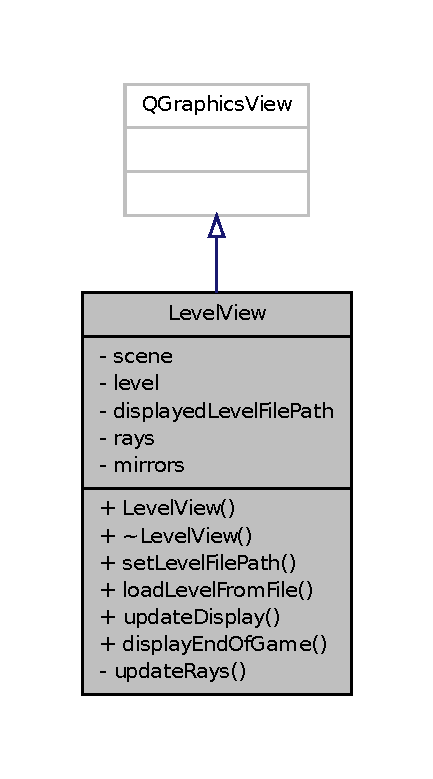
\includegraphics[width=208pt]{df/d61/classLevelView__inherit__graph}
\end{center}
\end{figure}


Graphe de collaboration de Level\+View\+:\nopagebreak
\begin{figure}[H]
\begin{center}
\leavevmode
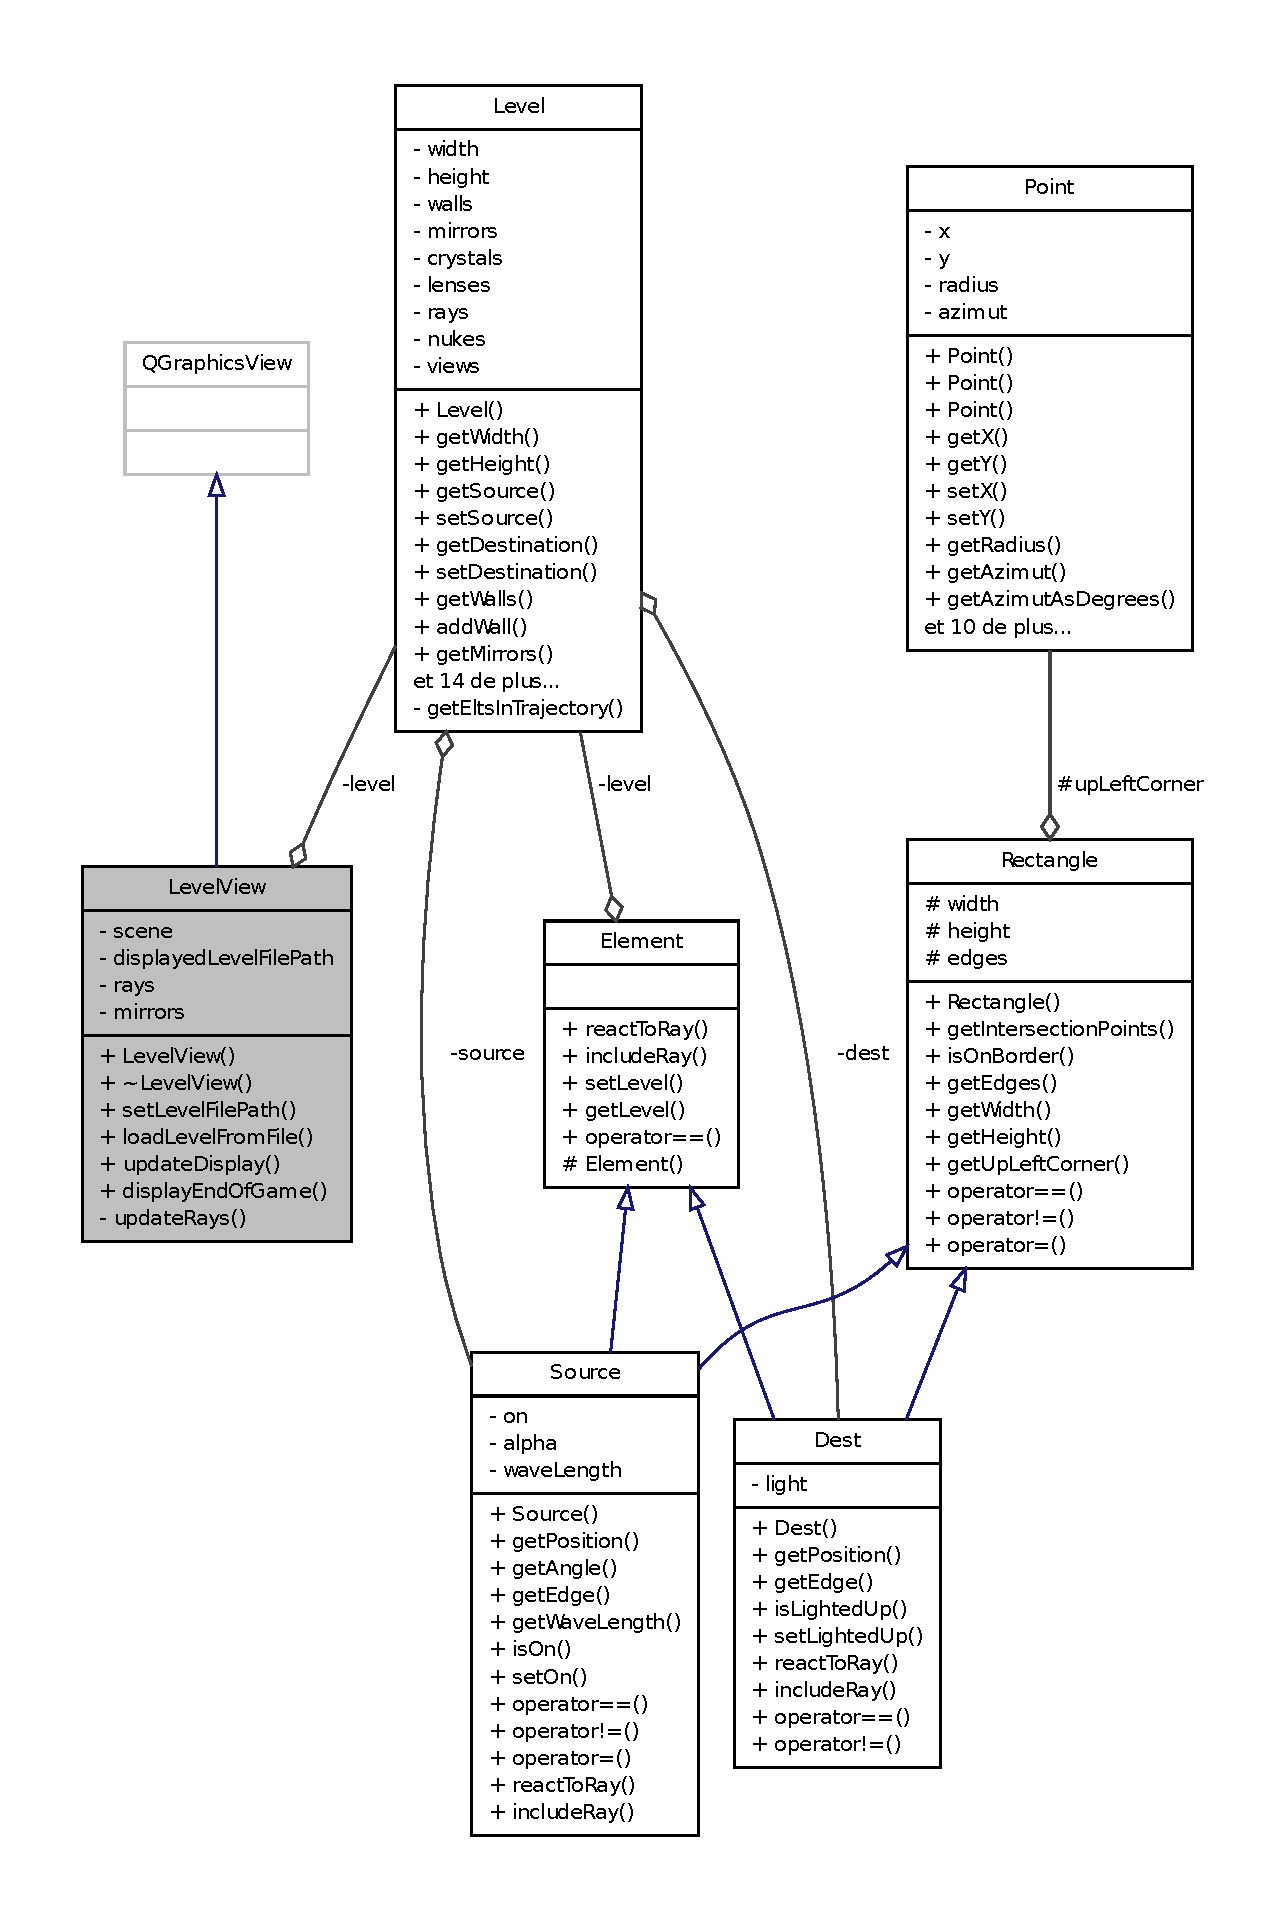
\includegraphics[width=350pt]{dd/d3d/classLevelView__coll__graph}
\end{center}
\end{figure}


\subsection{Documentation des constructeurs et destructeur}
\hypertarget{classLevelView_a1537183269cd26f8341f7e2eb80545d3}{}\index{Level\+View@{Level\+View}!Level\+View@{Level\+View}}
\index{Level\+View@{Level\+View}!Level\+View@{Level\+View}}
\subsubsection[{Level\+View(\+Q\+Widget $\ast$=0)}]{\setlength{\rightskip}{0pt plus 5cm}Level\+View\+::\+Level\+View (
\begin{DoxyParamCaption}
\item[{Q\+Widget $\ast$}]{ = {\ttfamily 0}}
\end{DoxyParamCaption}
)\hspace{0.3cm}{\ttfamily [explicit]}}\label{classLevelView_a1537183269cd26f8341f7e2eb80545d3}


Permet de créer une vue du niveau. 


\begin{DoxyParams}{Paramètres}
{\em parent} & L\textquotesingle{}objet graphique parent. \\
\hline
\end{DoxyParams}
\hypertarget{classLevelView_a8a68c0e4a47fc91422c2d1a22c735ea4}{}\index{Level\+View@{Level\+View}!````~Level\+View@{$\sim$\+Level\+View}}
\index{````~Level\+View@{$\sim$\+Level\+View}!Level\+View@{Level\+View}}
\subsubsection[{$\sim$\+Level\+View()}]{\setlength{\rightskip}{0pt plus 5cm}Level\+View\+::$\sim$\+Level\+View (
\begin{DoxyParamCaption}
{}
\end{DoxyParamCaption}
)}\label{classLevelView_a8a68c0e4a47fc91422c2d1a22c735ea4}


\subsection{Documentation des fonctions membres}
\hypertarget{classLevelView_ad6ea3472fed0f3aa469779b6efac3b41}{}\index{Level\+View@{Level\+View}!display\+End\+Of\+Game@{display\+End\+Of\+Game}}
\index{display\+End\+Of\+Game@{display\+End\+Of\+Game}!Level\+View@{Level\+View}}
\subsubsection[{display\+End\+Of\+Game}]{\setlength{\rightskip}{0pt plus 5cm}void Level\+View\+::display\+End\+Of\+Game (
\begin{DoxyParamCaption}
{}
\end{DoxyParamCaption}
)\hspace{0.3cm}{\ttfamily [slot]}}\label{classLevelView_ad6ea3472fed0f3aa469779b6efac3b41}


Permet d\textquotesingle{}afficher une boite de dialogue informant l\textquotesingle{}utilisateur de la fin du jeu. 

\hypertarget{classLevelView_a3953bf386139bae926640e8c9e90b5fe}{}\index{Level\+View@{Level\+View}!displaying\+Started@{displaying\+Started}}
\index{displaying\+Started@{displaying\+Started}!Level\+View@{Level\+View}}
\subsubsection[{displaying\+Started}]{\setlength{\rightskip}{0pt plus 5cm}void Level\+View\+::displaying\+Started (
\begin{DoxyParamCaption}
{}
\end{DoxyParamCaption}
)\hspace{0.3cm}{\ttfamily [signal]}}\label{classLevelView_a3953bf386139bae926640e8c9e90b5fe}


Signale que le niveau doit être affiché. 

\hypertarget{classLevelView_a4e35d1b0b0fa00a1a4c602da15471359}{}\index{Level\+View@{Level\+View}!displaying\+Stopped@{displaying\+Stopped}}
\index{displaying\+Stopped@{displaying\+Stopped}!Level\+View@{Level\+View}}
\subsubsection[{displaying\+Stopped}]{\setlength{\rightskip}{0pt plus 5cm}void Level\+View\+::displaying\+Stopped (
\begin{DoxyParamCaption}
{}
\end{DoxyParamCaption}
)\hspace{0.3cm}{\ttfamily [signal]}}\label{classLevelView_a4e35d1b0b0fa00a1a4c602da15471359}


Signale que le niveau ne doit plus être affiché. 

\hypertarget{classLevelView_a3bded54066b2ce49cf972b16d03817bb}{}\index{Level\+View@{Level\+View}!load\+Level\+From\+File@{load\+Level\+From\+File}}
\index{load\+Level\+From\+File@{load\+Level\+From\+File}!Level\+View@{Level\+View}}
\subsubsection[{load\+Level\+From\+File}]{\setlength{\rightskip}{0pt plus 5cm}void Level\+View\+::load\+Level\+From\+File (
\begin{DoxyParamCaption}
{}
\end{DoxyParamCaption}
)\hspace{0.3cm}{\ttfamily [slot]}}\label{classLevelView_a3bded54066b2ce49cf972b16d03817bb}


Permet d\textquotesingle{}afficher le fichier niveau dont la vue courante contient le chemin en attribut. 

\hypertarget{classLevelView_ae8298aa5d3163d7cc1343adbb2676d8a}{}\index{Level\+View@{Level\+View}!set\+Level\+File\+Path@{set\+Level\+File\+Path}}
\index{set\+Level\+File\+Path@{set\+Level\+File\+Path}!Level\+View@{Level\+View}}
\subsubsection[{set\+Level\+File\+Path}]{\setlength{\rightskip}{0pt plus 5cm}void Level\+View\+::set\+Level\+File\+Path (
\begin{DoxyParamCaption}
\item[{const Q\+String}]{}
\end{DoxyParamCaption}
)\hspace{0.3cm}{\ttfamily [slot]}}\label{classLevelView_ae8298aa5d3163d7cc1343adbb2676d8a}


Permet de changer le fichier de niveau et d\textquotesingle{}afficher ce niveau. 


\begin{DoxyParams}{Paramètres}
{\em level\+File} & chemin vers le fichier du nouveau niveau à afficher. \\
\hline
\end{DoxyParams}
\hypertarget{classLevelView_a3ada0dd54a12cc91a31113dd83553f3a}{}\index{Level\+View@{Level\+View}!update\+Display@{update\+Display}}
\index{update\+Display@{update\+Display}!Level\+View@{Level\+View}}
\subsubsection[{update\+Display}]{\setlength{\rightskip}{0pt plus 5cm}void Level\+View\+::update\+Display (
\begin{DoxyParamCaption}
{}
\end{DoxyParamCaption}
)\hspace{0.3cm}{\ttfamily [slot]}}\label{classLevelView_a3ada0dd54a12cc91a31113dd83553f3a}


Permet de rafraichir l\textquotesingle{}affichage lorsque le niveau change d\textquotesingle{}état. 

\hypertarget{classLevelView_a253e8066d8b1cd5c02f6f752b6497462}{}\index{Level\+View@{Level\+View}!update\+Rays@{update\+Rays}}
\index{update\+Rays@{update\+Rays}!Level\+View@{Level\+View}}
\subsubsection[{update\+Rays()}]{\setlength{\rightskip}{0pt plus 5cm}void Level\+View\+::update\+Rays (
\begin{DoxyParamCaption}
{}
\end{DoxyParamCaption}
)\hspace{0.3cm}{\ttfamily [private]}}\label{classLevelView_a253e8066d8b1cd5c02f6f752b6497462}


Permet de mettre à jour l\textquotesingle{}affichage des rayons. 



\subsection{Documentation des données membres}
\hypertarget{classLevelView_a826d9224c5bbbecb5c02b7734d0b8137}{}\index{Level\+View@{Level\+View}!displayed\+Level\+File\+Path@{displayed\+Level\+File\+Path}}
\index{displayed\+Level\+File\+Path@{displayed\+Level\+File\+Path}!Level\+View@{Level\+View}}
\subsubsection[{displayed\+Level\+File\+Path}]{\setlength{\rightskip}{0pt plus 5cm}std\+::string Level\+View\+::displayed\+Level\+File\+Path\hspace{0.3cm}{\ttfamily [private]}}\label{classLevelView_a826d9224c5bbbecb5c02b7734d0b8137}


Le chemin du fichier chargé par l\textquotesingle{}utilisateur. 



Définition à la ligne 36 du fichier levelview.\+hpp.

\hypertarget{classLevelView_ab51fb77e921a425c79b9671ebb8718e2}{}\index{Level\+View@{Level\+View}!level@{level}}
\index{level@{level}!Level\+View@{Level\+View}}
\subsubsection[{level}]{\setlength{\rightskip}{0pt plus 5cm}{\bf Level}$\ast$ Level\+View\+::level\hspace{0.3cm}{\ttfamily [private]}}\label{classLevelView_ab51fb77e921a425c79b9671ebb8718e2}


Le niveau quel la vue observe. 



Définition à la ligne 31 du fichier levelview.\+hpp.

\hypertarget{classLevelView_ad530e6ab8704e9201efe04bf98ff44e9}{}\index{Level\+View@{Level\+View}!mirrors@{mirrors}}
\index{mirrors@{mirrors}!Level\+View@{Level\+View}}
\subsubsection[{mirrors}]{\setlength{\rightskip}{0pt plus 5cm}std\+::vector$<${\bf Mirror\+View} $\ast$$>$ Level\+View\+::mirrors\hspace{0.3cm}{\ttfamily [private]}}\label{classLevelView_ad530e6ab8704e9201efe04bf98ff44e9}


L\textquotesingle{}ensemble des miroirs dessinés. 



Définition à la ligne 46 du fichier levelview.\+hpp.

\hypertarget{classLevelView_a79c31b19d94522a4756bcf0bbae0c1a1}{}\index{Level\+View@{Level\+View}!rays@{rays}}
\index{rays@{rays}!Level\+View@{Level\+View}}
\subsubsection[{rays}]{\setlength{\rightskip}{0pt plus 5cm}std\+::vector$<$Q\+Graphics\+Line\+Item $\ast$$>$ Level\+View\+::rays\hspace{0.3cm}{\ttfamily [private]}}\label{classLevelView_a79c31b19d94522a4756bcf0bbae0c1a1}


L\textquotesingle{}ensemble des rayons dessinés. 



Définition à la ligne 41 du fichier levelview.\+hpp.

\hypertarget{classLevelView_a81030b9faa8743a629553447bfb982ea}{}\index{Level\+View@{Level\+View}!scene@{scene}}
\index{scene@{scene}!Level\+View@{Level\+View}}
\subsubsection[{scene}]{\setlength{\rightskip}{0pt plus 5cm}Q\+Graphics\+Scene$\ast$ Level\+View\+::scene\hspace{0.3cm}{\ttfamily [private]}}\label{classLevelView_a81030b9faa8743a629553447bfb982ea}


La scène qui comportera l\textquotesingle{}ensemble des éléments graphiques de la partie. 



Définition à la ligne 26 du fichier levelview.\+hpp.



La documentation de cette classe a été générée à partir du fichier suivant \+:\begin{DoxyCompactItemize}
\item 
view/windows/\hyperlink{levelview_8hpp}{levelview.\+hpp}\end{DoxyCompactItemize}

\hypertarget{classLine}{}\section{Référence de la classe Line}
\label{classLine}\index{Line@{Line}}


Représente une droite sous la forme de son équation complète; $ eq \equiv y = slope \cdot x + indepTerm $.  




{\ttfamily \#include $<$line.\+hpp$>$}

\subsection*{Fonctions membres publiques}
\begin{DoxyCompactItemize}
\item 
\hyperlink{classLine_a51acfb27d7778c0f96624edc27dab5c7}{Line} (double, double, double=0)
\begin{DoxyCompactList}\small\item\em Permet de construire une nouvelle droite initialisée. \end{DoxyCompactList}\item 
\hyperlink{classLine_a13562b07c6a09b1bc7720a6c4f77fb3e}{Line} (const \hyperlink{classPoint}{Point} \&, const \hyperlink{classPoint}{Point} \&)
\begin{DoxyCompactList}\small\item\em Permet de construire une droite à partir de deux points. \end{DoxyCompactList}\item 
\hyperlink{classPoint}{Point} $\ast$ \hyperlink{classLine_a9449a6777c0d4783b2210c057ae1c811}{get\+Intersection\+Point} (const \hyperlink{classLine}{Line} \&) const 
\begin{DoxyCompactList}\small\item\em Permet d\textquotesingle{}obtenir le point d\textquotesingle{}intersection entre la droite et celle entrée en paramètre. \end{DoxyCompactList}\item 
bool \hyperlink{classLine_a36eaf7c0fcc008e1e72a1a82137f42a4}{includes} (const \hyperlink{classPoint}{Point} \&) const 
\begin{DoxyCompactList}\small\item\em Renseigne si le point entré en paramètre est inclus dans la droite. \end{DoxyCompactList}\item 
double \hyperlink{classLine_a9eab2739a90a731de04b385f483f68b3}{get\+Slope} () const 
\begin{DoxyCompactList}\small\item\em Permet d\textquotesingle{}obtenir la pente de la droite. \end{DoxyCompactList}\item 
double \hyperlink{classLine_a7a543f2f53ad54555a56c845375f2a7d}{get\+Indep\+Term} () const 
\begin{DoxyCompactList}\small\item\em Permet d\textquotesingle{}obtenir le terme indépendant. \end{DoxyCompactList}\item 
double \hyperlink{classLine_aa50bf9b9bc8fa001e6f33a3914e749af}{get\+X\+Value} () const 
\begin{DoxyCompactList}\small\item\em Permet de connaitre la valeur de x, cette valeur est incohérence si la droite n\textquotesingle{}est pas verticale. \end{DoxyCompactList}\item 
bool \hyperlink{classLine_adb1e4c411e63f9ac31f70648fa3149d7}{is\+Vertical} () const 
\begin{DoxyCompactList}\small\item\em Renseigne si la droite est verticale. \end{DoxyCompactList}\item 
double \hyperlink{classLine_a013de9d97b5c80dd2e52888022e58a5d}{find\+X} (const double) const 
\begin{DoxyCompactList}\small\item\em Permet de résoudre l\textquotesingle{}équation de la droite à partir d\textquotesingle{}une valeur de y entrée en paramètre. \end{DoxyCompactList}\item 
double \hyperlink{classLine_a6573ef5cdd6324971770d4a556fed4ae}{find\+Y} (const double) const 
\begin{DoxyCompactList}\small\item\em Permet de résoudre l\textquotesingle{}équation de la droite à partir d\textquotesingle{}une valeur de x entrée en paramètre. \end{DoxyCompactList}\item 
\hyperlink{classLine}{Line} \& \hyperlink{classLine_aff9faa550dc184fac56e3ef22439fdf9}{operator=} (const \hyperlink{classLine}{Line} \&)
\begin{DoxyCompactList}\small\item\em Permet de copier une ligne. \end{DoxyCompactList}\item 
bool \hyperlink{classLine_a5f1b6226cd499d6d209cda4b8517c9b7}{operator==} (const \hyperlink{classLine}{Line} \&) const 
\begin{DoxyCompactList}\small\item\em Permet de savoir si deux lignes sont identiques. \end{DoxyCompactList}\item 
bool \hyperlink{classLine_ae2cb0479252a7f5a2c163d1197fc990f}{operator!=} (const \hyperlink{classLine}{Line} \&) const 
\begin{DoxyCompactList}\small\item\em Permet de savoir si deux lignes sont différentes. \end{DoxyCompactList}\end{DoxyCompactItemize}
\subsection*{Attributs protégés}
\begin{DoxyCompactItemize}
\item 
double \hyperlink{classLine_a0aa35363f8285600b12ce54258338b8c}{slope}
\begin{DoxyCompactList}\small\item\em slope Valeur du coefficient angulaire de la droite. \end{DoxyCompactList}\item 
double \hyperlink{classLine_a6ea839b47ccf670770ebc7dff9f0dbba}{indep\+Term}
\begin{DoxyCompactList}\small\item\em indep\+Term Contient la valeur du terme indépendant de la droite. \end{DoxyCompactList}\item 
double \hyperlink{classLine_af8b70928b9624988c1c42f33af93391a}{x\+Value}
\begin{DoxyCompactList}\small\item\em x\+Value Contient la valeur de x lorsque la droite est verticale. \end{DoxyCompactList}\end{DoxyCompactItemize}


\subsection{Description détaillée}
Représente une droite sous la forme de son équation complète; $ eq \equiv y = slope \cdot x + indepTerm $. 

Définition à la ligne 13 du fichier line.\+hpp.



Graphe d\textquotesingle{}héritage de Line\+:\nopagebreak
\begin{figure}[H]
\begin{center}
\leavevmode
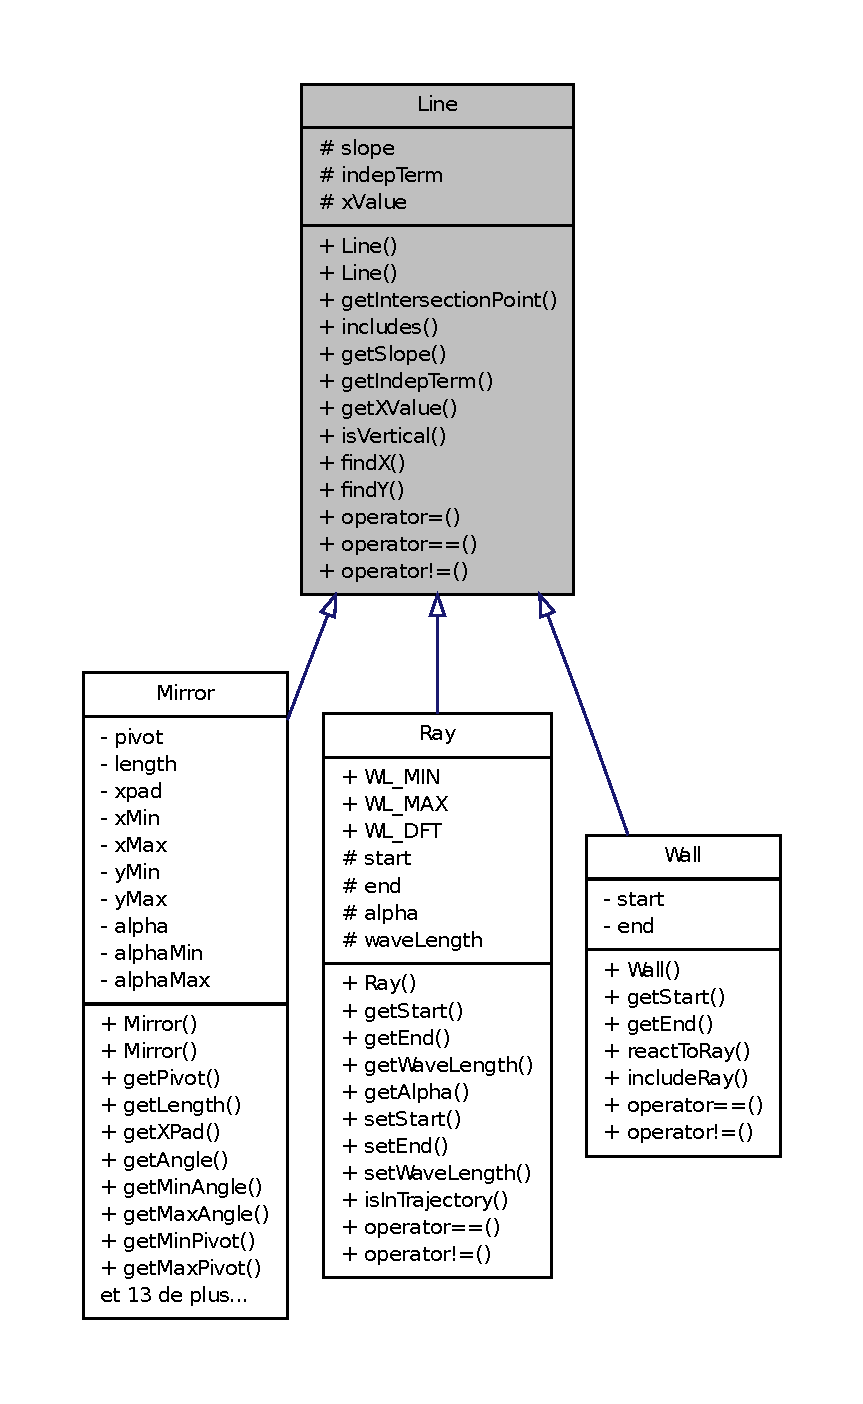
\includegraphics[height=550pt]{d4/d12/classLine__inherit__graph}
\end{center}
\end{figure}


Graphe de collaboration de Line\+:\nopagebreak
\begin{figure}[H]
\begin{center}
\leavevmode
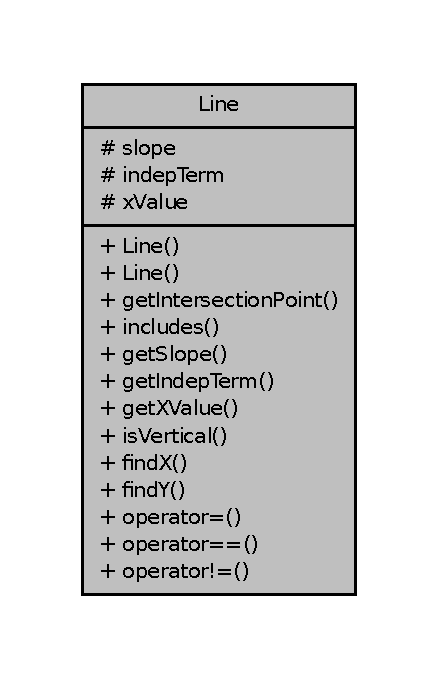
\includegraphics[width=210pt]{de/d2f/classLine__coll__graph}
\end{center}
\end{figure}


\subsection{Documentation des constructeurs et destructeur}
\hypertarget{classLine_a51acfb27d7778c0f96624edc27dab5c7}{}\index{Line@{Line}!Line@{Line}}
\index{Line@{Line}!Line@{Line}}
\subsubsection[{Line(double, double, double=0)}]{\setlength{\rightskip}{0pt plus 5cm}Line\+::\+Line (
\begin{DoxyParamCaption}
\item[{double}]{, }
\item[{double}]{, }
\item[{double}]{ = {\ttfamily 0}}
\end{DoxyParamCaption}
)}\label{classLine_a51acfb27d7778c0f96624edc27dab5c7}


Permet de construire une nouvelle droite initialisée. 


\begin{DoxyParams}{Paramètres}
{\em slope} & Pente de la droite. \\
\hline
{\em indep\+Term} & Terme indépendant de la droite. \\
\hline
{\em x\+Value} & Valeur de x si la droite est verticale. \\
\hline
\end{DoxyParams}
\hypertarget{classLine_a13562b07c6a09b1bc7720a6c4f77fb3e}{}\index{Line@{Line}!Line@{Line}}
\index{Line@{Line}!Line@{Line}}
\subsubsection[{Line(const Point \&, const Point \&)}]{\setlength{\rightskip}{0pt plus 5cm}Line\+::\+Line (
\begin{DoxyParamCaption}
\item[{const {\bf Point} \&}]{, }
\item[{const {\bf Point} \&}]{}
\end{DoxyParamCaption}
)}\label{classLine_a13562b07c6a09b1bc7720a6c4f77fb3e}


Permet de construire une droite à partir de deux points. 


\begin{DoxyParams}{Paramètres}
{\em start} & \hyperlink{classPoint}{Point} le plus près de l\textquotesingle{}origine au niveau de l\textquotesingle{}abscisse. \\
\hline
{\em end} & \hyperlink{classPoint}{Point} le plus éloigné de l\textquotesingle{}origine au niveau de l\textquotesingle{}abscisse. \\
\hline
\end{DoxyParams}


\subsection{Documentation des fonctions membres}
\hypertarget{classLine_a013de9d97b5c80dd2e52888022e58a5d}{}\index{Line@{Line}!find\+X@{find\+X}}
\index{find\+X@{find\+X}!Line@{Line}}
\subsubsection[{find\+X(const double) const }]{\setlength{\rightskip}{0pt plus 5cm}double Line\+::find\+X (
\begin{DoxyParamCaption}
\item[{const double}]{}
\end{DoxyParamCaption}
) const}\label{classLine_a013de9d97b5c80dd2e52888022e58a5d}


Permet de résoudre l\textquotesingle{}équation de la droite à partir d\textquotesingle{}une valeur de y entrée en paramètre. 


\begin{DoxyParams}{Paramètres}
{\em y} & Valeur de y pour résoudre l\textquotesingle{}équation de la droite.\\
\hline
\end{DoxyParams}
\begin{DoxyReturn}{Renvoie}
le valeur de x après résolution de l\textquotesingle{}équation de la droite à partir d\textquotesingle{}une valeur de y entrée en paramètre. 
\end{DoxyReturn}
\hypertarget{classLine_a6573ef5cdd6324971770d4a556fed4ae}{}\index{Line@{Line}!find\+Y@{find\+Y}}
\index{find\+Y@{find\+Y}!Line@{Line}}
\subsubsection[{find\+Y(const double) const }]{\setlength{\rightskip}{0pt plus 5cm}double Line\+::find\+Y (
\begin{DoxyParamCaption}
\item[{const double}]{}
\end{DoxyParamCaption}
) const}\label{classLine_a6573ef5cdd6324971770d4a556fed4ae}


Permet de résoudre l\textquotesingle{}équation de la droite à partir d\textquotesingle{}une valeur de x entrée en paramètre. 


\begin{DoxyParams}{Paramètres}
{\em x} & Valeur de x pour résoudre l\textquotesingle{}équation de la droite.\\
\hline
\end{DoxyParams}
\begin{DoxyReturn}{Renvoie}
la valeur de y après résolution de l\textquotesingle{}équation de la droite à partir d\textquotesingle{}une valeur de y entrée en paramètre. 
\end{DoxyReturn}
\hypertarget{classLine_a7a543f2f53ad54555a56c845375f2a7d}{}\index{Line@{Line}!get\+Indep\+Term@{get\+Indep\+Term}}
\index{get\+Indep\+Term@{get\+Indep\+Term}!Line@{Line}}
\subsubsection[{get\+Indep\+Term() const }]{\setlength{\rightskip}{0pt plus 5cm}double Line\+::get\+Indep\+Term (
\begin{DoxyParamCaption}
{}
\end{DoxyParamCaption}
) const\hspace{0.3cm}{\ttfamily [inline]}}\label{classLine_a7a543f2f53ad54555a56c845375f2a7d}


Permet d\textquotesingle{}obtenir le terme indépendant. 

\begin{DoxyReturn}{Renvoie}
Le terme indépendant. 
\end{DoxyReturn}


Définition à la ligne 160 du fichier line.\+hpp.



Références indep\+Term.


\begin{DoxyCode}
161 \{
162     \textcolor{keywordflow}{return} this->\hyperlink{classLine_a6ea839b47ccf670770ebc7dff9f0dbba}{indepTerm};
163 \}
\end{DoxyCode}
\hypertarget{classLine_a9449a6777c0d4783b2210c057ae1c811}{}\index{Line@{Line}!get\+Intersection\+Point@{get\+Intersection\+Point}}
\index{get\+Intersection\+Point@{get\+Intersection\+Point}!Line@{Line}}
\subsubsection[{get\+Intersection\+Point(const Line \&) const }]{\setlength{\rightskip}{0pt plus 5cm}{\bf Point}$\ast$ Line\+::get\+Intersection\+Point (
\begin{DoxyParamCaption}
\item[{const {\bf Line} \&}]{}
\end{DoxyParamCaption}
) const}\label{classLine_a9449a6777c0d4783b2210c057ae1c811}


Permet d\textquotesingle{}obtenir le point d\textquotesingle{}intersection entre la droite et celle entrée en paramètre. 


\begin{DoxyParams}{Paramètres}
{\em line} & Droite dont on désire obtenir le point d\textquotesingle{}intersection avec la droite courante.\\
\hline
\end{DoxyParams}
\begin{DoxyReturn}{Renvoie}
Un pointeur vers un le point d\textquotesingle{}intersection entre la droite et celle entrée en paramètre si il existe, un pointeur nul sinon. 
\end{DoxyReturn}
\hypertarget{classLine_a9eab2739a90a731de04b385f483f68b3}{}\index{Line@{Line}!get\+Slope@{get\+Slope}}
\index{get\+Slope@{get\+Slope}!Line@{Line}}
\subsubsection[{get\+Slope() const }]{\setlength{\rightskip}{0pt plus 5cm}double Line\+::get\+Slope (
\begin{DoxyParamCaption}
{}
\end{DoxyParamCaption}
) const\hspace{0.3cm}{\ttfamily [inline]}}\label{classLine_a9eab2739a90a731de04b385f483f68b3}


Permet d\textquotesingle{}obtenir la pente de la droite. 

\begin{DoxyReturn}{Renvoie}
La pente de la droite. 
\end{DoxyReturn}


Définition à la ligne 155 du fichier line.\+hpp.



Références slope.


\begin{DoxyCode}
156 \{
157     \textcolor{keywordflow}{return} this->\hyperlink{classLine_a0aa35363f8285600b12ce54258338b8c}{slope};
158 \}
\end{DoxyCode}
\hypertarget{classLine_aa50bf9b9bc8fa001e6f33a3914e749af}{}\index{Line@{Line}!get\+X\+Value@{get\+X\+Value}}
\index{get\+X\+Value@{get\+X\+Value}!Line@{Line}}
\subsubsection[{get\+X\+Value() const }]{\setlength{\rightskip}{0pt plus 5cm}double Line\+::get\+X\+Value (
\begin{DoxyParamCaption}
{}
\end{DoxyParamCaption}
) const\hspace{0.3cm}{\ttfamily [inline]}}\label{classLine_aa50bf9b9bc8fa001e6f33a3914e749af}


Permet de connaitre la valeur de x, cette valeur est incohérence si la droite n\textquotesingle{}est pas verticale. 

\begin{DoxyReturn}{Renvoie}
La valeur de x si la droite est verticale. 
\end{DoxyReturn}


Définition à la ligne 165 du fichier line.\+hpp.



Références x\+Value.


\begin{DoxyCode}
166 \{
167     \textcolor{keywordflow}{return} this->\hyperlink{classLine_af8b70928b9624988c1c42f33af93391a}{xValue};
168 \}
\end{DoxyCode}
\hypertarget{classLine_a36eaf7c0fcc008e1e72a1a82137f42a4}{}\index{Line@{Line}!includes@{includes}}
\index{includes@{includes}!Line@{Line}}
\subsubsection[{includes(const Point \&) const }]{\setlength{\rightskip}{0pt plus 5cm}bool Line\+::includes (
\begin{DoxyParamCaption}
\item[{const {\bf Point} \&}]{}
\end{DoxyParamCaption}
) const}\label{classLine_a36eaf7c0fcc008e1e72a1a82137f42a4}


Renseigne si le point entré en paramètre est inclus dans la droite. 


\begin{DoxyParams}{Paramètres}
{\em point} & \hyperlink{classPoint}{Point} dont on désire savoir s\textquotesingle{}il est inclus dans la droite.\\
\hline
\end{DoxyParams}
\begin{DoxyReturn}{Renvoie}
{\ttfamily true} si le point entré en paramètre est inclus dans la droite. 
\end{DoxyReturn}
\hypertarget{classLine_adb1e4c411e63f9ac31f70648fa3149d7}{}\index{Line@{Line}!is\+Vertical@{is\+Vertical}}
\index{is\+Vertical@{is\+Vertical}!Line@{Line}}
\subsubsection[{is\+Vertical() const }]{\setlength{\rightskip}{0pt plus 5cm}bool Line\+::is\+Vertical (
\begin{DoxyParamCaption}
{}
\end{DoxyParamCaption}
) const}\label{classLine_adb1e4c411e63f9ac31f70648fa3149d7}


Renseigne si la droite est verticale. 

\begin{DoxyReturn}{Renvoie}
{\ttfamily true} Si la droite est verticale. 
\end{DoxyReturn}
\hypertarget{classLine_ae2cb0479252a7f5a2c163d1197fc990f}{}\index{Line@{Line}!operator"!=@{operator"!=}}
\index{operator"!=@{operator"!=}!Line@{Line}}
\subsubsection[{operator"!=(const Line \&) const }]{\setlength{\rightskip}{0pt plus 5cm}bool Line\+::operator!= (
\begin{DoxyParamCaption}
\item[{const {\bf Line} \&}]{}
\end{DoxyParamCaption}
) const}\label{classLine_ae2cb0479252a7f5a2c163d1197fc990f}


Permet de savoir si deux lignes sont différentes. 

\begin{DoxyReturn}{Renvoie}
{\ttfamily true} Si deux lignes sont différentes. 
\end{DoxyReturn}
\hypertarget{classLine_aff9faa550dc184fac56e3ef22439fdf9}{}\index{Line@{Line}!operator=@{operator=}}
\index{operator=@{operator=}!Line@{Line}}
\subsubsection[{operator=(const Line \&)}]{\setlength{\rightskip}{0pt plus 5cm}{\bf Line}\& Line\+::operator= (
\begin{DoxyParamCaption}
\item[{const {\bf Line} \&}]{}
\end{DoxyParamCaption}
)}\label{classLine_aff9faa550dc184fac56e3ef22439fdf9}


Permet de copier une ligne. 

\begin{DoxyReturn}{Renvoie}
La ligne courante représentant la ligne passée en paramètre. 
\end{DoxyReturn}
\hypertarget{classLine_a5f1b6226cd499d6d209cda4b8517c9b7}{}\index{Line@{Line}!operator==@{operator==}}
\index{operator==@{operator==}!Line@{Line}}
\subsubsection[{operator==(const Line \&) const }]{\setlength{\rightskip}{0pt plus 5cm}bool Line\+::operator== (
\begin{DoxyParamCaption}
\item[{const {\bf Line} \&}]{}
\end{DoxyParamCaption}
) const}\label{classLine_a5f1b6226cd499d6d209cda4b8517c9b7}


Permet de savoir si deux lignes sont identiques. 

\begin{DoxyReturn}{Renvoie}
{\ttfamily true} Si deux lignes sont identiques. 
\end{DoxyReturn}


\subsection{Documentation des données membres}
\hypertarget{classLine_a6ea839b47ccf670770ebc7dff9f0dbba}{}\index{Line@{Line}!indep\+Term@{indep\+Term}}
\index{indep\+Term@{indep\+Term}!Line@{Line}}
\subsubsection[{indep\+Term}]{\setlength{\rightskip}{0pt plus 5cm}double Line\+::indep\+Term\hspace{0.3cm}{\ttfamily [protected]}}\label{classLine_a6ea839b47ccf670770ebc7dff9f0dbba}


indep\+Term Contient la valeur du terme indépendant de la droite. 



Définition à la ligne 26 du fichier line.\+hpp.



Référencé par get\+Indep\+Term().

\hypertarget{classLine_a0aa35363f8285600b12ce54258338b8c}{}\index{Line@{Line}!slope@{slope}}
\index{slope@{slope}!Line@{Line}}
\subsubsection[{slope}]{\setlength{\rightskip}{0pt plus 5cm}double Line\+::slope\hspace{0.3cm}{\ttfamily [protected]}}\label{classLine_a0aa35363f8285600b12ce54258338b8c}


slope Valeur du coefficient angulaire de la droite. 



Définition à la ligne 21 du fichier line.\+hpp.



Référencé par get\+Slope().

\hypertarget{classLine_af8b70928b9624988c1c42f33af93391a}{}\index{Line@{Line}!x\+Value@{x\+Value}}
\index{x\+Value@{x\+Value}!Line@{Line}}
\subsubsection[{x\+Value}]{\setlength{\rightskip}{0pt plus 5cm}double Line\+::x\+Value\hspace{0.3cm}{\ttfamily [protected]}}\label{classLine_af8b70928b9624988c1c42f33af93391a}


x\+Value Contient la valeur de x lorsque la droite est verticale. 



Définition à la ligne 31 du fichier line.\+hpp.



Référencé par get\+X\+Value().



La documentation de cette classe a été générée à partir du fichier suivant \+:\begin{DoxyCompactItemize}
\item 
model/geometry/\hyperlink{line_8hpp}{line.\+hpp}\end{DoxyCompactItemize}

\hypertarget{classMainMenu}{}\section{Référence de la classe Main\+Menu}
\label{classMainMenu}\index{Main\+Menu@{Main\+Menu}}


Cette classe représente le menu principal du jeu permettant de.  




{\ttfamily \#include $<$mainmenu.\+hpp$>$}

\subsection*{Connecteurs publics}
\begin{DoxyCompactItemize}
\item 
void \hyperlink{classMainMenu_ab615dd0e5129bf9df28a1f493baad741}{select\+New\+Level\+File} ()
\begin{DoxyCompactList}\small\item\em Permet de faire sélectionner un fichier de niveau par l\textquotesingle{}utilisateur. \end{DoxyCompactList}\item 
void \hyperlink{classMainMenu_af449ad4f8eb0d941fb4e8bc2a352fc48}{display\+Rules} ()
\begin{DoxyCompactList}\small\item\em Permet d\textquotesingle{}afficher une fenêtre de dialogue contenant les règles et les commandes du jeu. \end{DoxyCompactList}\end{DoxyCompactItemize}
\subsection*{Signaux}
\begin{DoxyCompactItemize}
\item 
void \hyperlink{classMainMenu_acad34fb589f6f168930cbc1b89ccf7cb}{new\+Level\+File\+Selected} (const Q\+String)
\begin{DoxyCompactList}\small\item\em Signale qu\textquotesingle{}un nouveau fichier a été sélectionné par l\textquotesingle{}utilisateur. \end{DoxyCompactList}\end{DoxyCompactItemize}
\subsection*{Fonctions membres publiques}
\begin{DoxyCompactItemize}
\item 
\hyperlink{classMainMenu_a69707caeb524bd0600a0d05613108af5}{Main\+Menu} (Q\+Widget $\ast$=0)
\begin{DoxyCompactList}\small\item\em Permet de créer un menu du jeu. \end{DoxyCompactList}\item 
\hyperlink{classMainMenu_a0a19ddba3ac52bf39c09b579171c98f2}{$\sim$\+Main\+Menu} ()
\end{DoxyCompactItemize}
\subsection*{Fonctions membres privées}
\begin{DoxyCompactItemize}
\item 
Q\+Label $\ast$ \hyperlink{classMainMenu_aa3dd35ff0093ab766b10ef6a0d1586a1}{set\+Logo} ()
\end{DoxyCompactItemize}


\subsection{Description détaillée}
Cette classe représente le menu principal du jeu permettant de. 


\begin{DoxyItemize}
\item sélectionner un niveau à jouer,  
\item lire les règles du jeu,  
\item quitter le jeu.  
\end{DoxyItemize}

Définition à la ligne 15 du fichier mainmenu.\+hpp.



Graphe d\textquotesingle{}héritage de Main\+Menu\+:\nopagebreak
\begin{figure}[H]
\begin{center}
\leavevmode
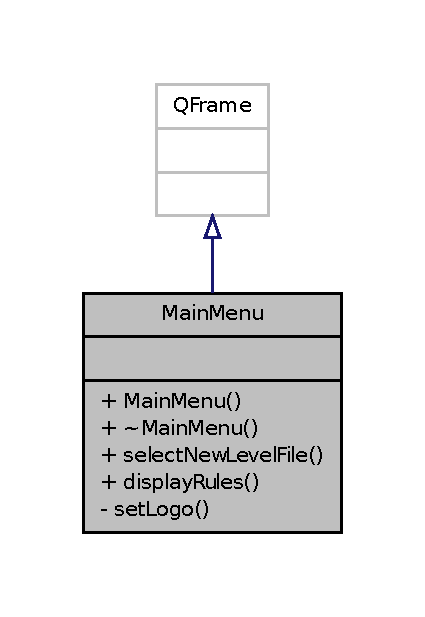
\includegraphics[width=204pt]{db/d55/classMainMenu__inherit__graph}
\end{center}
\end{figure}


Graphe de collaboration de Main\+Menu\+:\nopagebreak
\begin{figure}[H]
\begin{center}
\leavevmode
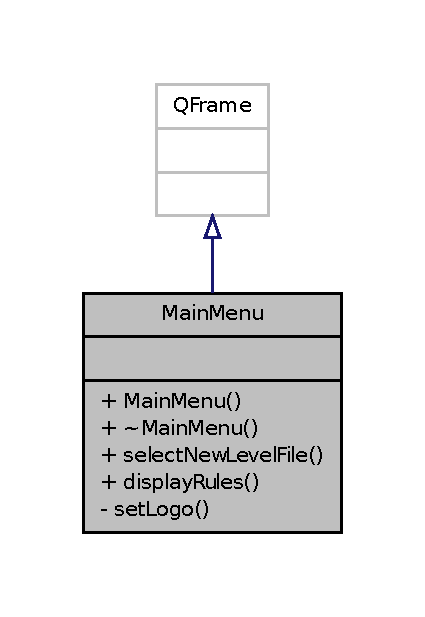
\includegraphics[width=204pt]{d8/d60/classMainMenu__coll__graph}
\end{center}
\end{figure}


\subsection{Documentation des constructeurs et destructeur}
\hypertarget{classMainMenu_a69707caeb524bd0600a0d05613108af5}{}\index{Main\+Menu@{Main\+Menu}!Main\+Menu@{Main\+Menu}}
\index{Main\+Menu@{Main\+Menu}!Main\+Menu@{Main\+Menu}}
\subsubsection[{Main\+Menu(\+Q\+Widget $\ast$=0)}]{\setlength{\rightskip}{0pt plus 5cm}Main\+Menu\+::\+Main\+Menu (
\begin{DoxyParamCaption}
\item[{Q\+Widget $\ast$}]{ = {\ttfamily 0}}
\end{DoxyParamCaption}
)\hspace{0.3cm}{\ttfamily [explicit]}}\label{classMainMenu_a69707caeb524bd0600a0d05613108af5}


Permet de créer un menu du jeu. 

\hypertarget{classMainMenu_a0a19ddba3ac52bf39c09b579171c98f2}{}\index{Main\+Menu@{Main\+Menu}!````~Main\+Menu@{$\sim$\+Main\+Menu}}
\index{````~Main\+Menu@{$\sim$\+Main\+Menu}!Main\+Menu@{Main\+Menu}}
\subsubsection[{$\sim$\+Main\+Menu()}]{\setlength{\rightskip}{0pt plus 5cm}Main\+Menu\+::$\sim$\+Main\+Menu (
\begin{DoxyParamCaption}
{}
\end{DoxyParamCaption}
)}\label{classMainMenu_a0a19ddba3ac52bf39c09b579171c98f2}


\subsection{Documentation des fonctions membres}
\hypertarget{classMainMenu_af449ad4f8eb0d941fb4e8bc2a352fc48}{}\index{Main\+Menu@{Main\+Menu}!display\+Rules@{display\+Rules}}
\index{display\+Rules@{display\+Rules}!Main\+Menu@{Main\+Menu}}
\subsubsection[{display\+Rules}]{\setlength{\rightskip}{0pt plus 5cm}void Main\+Menu\+::display\+Rules (
\begin{DoxyParamCaption}
{}
\end{DoxyParamCaption}
)\hspace{0.3cm}{\ttfamily [slot]}}\label{classMainMenu_af449ad4f8eb0d941fb4e8bc2a352fc48}


Permet d\textquotesingle{}afficher une fenêtre de dialogue contenant les règles et les commandes du jeu. 

\hypertarget{classMainMenu_acad34fb589f6f168930cbc1b89ccf7cb}{}\index{Main\+Menu@{Main\+Menu}!new\+Level\+File\+Selected@{new\+Level\+File\+Selected}}
\index{new\+Level\+File\+Selected@{new\+Level\+File\+Selected}!Main\+Menu@{Main\+Menu}}
\subsubsection[{new\+Level\+File\+Selected}]{\setlength{\rightskip}{0pt plus 5cm}void Main\+Menu\+::new\+Level\+File\+Selected (
\begin{DoxyParamCaption}
\item[{const Q\+String}]{}
\end{DoxyParamCaption}
)\hspace{0.3cm}{\ttfamily [signal]}}\label{classMainMenu_acad34fb589f6f168930cbc1b89ccf7cb}


Signale qu\textquotesingle{}un nouveau fichier a été sélectionné par l\textquotesingle{}utilisateur. 


\begin{DoxyParams}{Paramètres}
{\em new\+Level\+File} & Chemin vers le nouveau fichier sélectionné. \\
\hline
\end{DoxyParams}
\hypertarget{classMainMenu_ab615dd0e5129bf9df28a1f493baad741}{}\index{Main\+Menu@{Main\+Menu}!select\+New\+Level\+File@{select\+New\+Level\+File}}
\index{select\+New\+Level\+File@{select\+New\+Level\+File}!Main\+Menu@{Main\+Menu}}
\subsubsection[{select\+New\+Level\+File}]{\setlength{\rightskip}{0pt plus 5cm}void Main\+Menu\+::select\+New\+Level\+File (
\begin{DoxyParamCaption}
{}
\end{DoxyParamCaption}
)\hspace{0.3cm}{\ttfamily [slot]}}\label{classMainMenu_ab615dd0e5129bf9df28a1f493baad741}


Permet de faire sélectionner un fichier de niveau par l\textquotesingle{}utilisateur. 


\begin{DoxyParams}{Paramètres}
{\em new\+Level\+File} & Chemin vers le nouveau fichier sélectionné. \\
\hline
\end{DoxyParams}
\hypertarget{classMainMenu_aa3dd35ff0093ab766b10ef6a0d1586a1}{}\index{Main\+Menu@{Main\+Menu}!set\+Logo@{set\+Logo}}
\index{set\+Logo@{set\+Logo}!Main\+Menu@{Main\+Menu}}
\subsubsection[{set\+Logo()}]{\setlength{\rightskip}{0pt plus 5cm}Q\+Label$\ast$ Main\+Menu\+::set\+Logo (
\begin{DoxyParamCaption}
{}
\end{DoxyParamCaption}
)\hspace{0.3cm}{\ttfamily [private]}}\label{classMainMenu_aa3dd35ff0093ab766b10ef6a0d1586a1}


La documentation de cette classe a été générée à partir du fichier suivant \+:\begin{DoxyCompactItemize}
\item 
view/windows/\hyperlink{mainmenu_8hpp}{mainmenu.\+hpp}\end{DoxyCompactItemize}

\hypertarget{classMainWindow}{}\section{Référence de la classe Main\+Window}
\label{classMainWindow}\index{Main\+Window@{Main\+Window}}


Cette classe est la fenêtre principale du jeu qui englobe toutes les autres vues.  




{\ttfamily \#include $<$mainwindow.\+hpp$>$}

\subsection*{Connecteurs publics}
\begin{DoxyCompactItemize}
\item 
void \hyperlink{classMainWindow_a378316f6c8670867a82a7806cfa050d8}{display\+Main\+Menu} ()
\begin{DoxyCompactList}\small\item\em Permet d\textquotesingle{}afficher le menu principal du jeu. \end{DoxyCompactList}\item 
void \hyperlink{classMainWindow_a0aadedf51803aeb60945aa0f809ddaa0}{display\+Level} ()
\begin{DoxyCompactList}\small\item\em Permet d\textquotesingle{}afficher le niveau. \end{DoxyCompactList}\end{DoxyCompactItemize}
\subsection*{Fonctions membres publiques}
\begin{DoxyCompactItemize}
\item 
\hyperlink{classMainWindow_a2022dfcfcd6eeba03aec9f1e6eb3ece0}{Main\+Window} (Q\+Widget $\ast$=0)
\begin{DoxyCompactList}\small\item\em Créer une fenêtre principale du jeu. \end{DoxyCompactList}\item 
\hyperlink{classMainWindow_ae98d00a93bc118200eeef9f9bba1dba7}{$\sim$\+Main\+Window} ()
\end{DoxyCompactItemize}
\subsection*{Fonctions membres privées}
\begin{DoxyCompactItemize}
\item 
void \hyperlink{classMainWindow_a306206f30c08b874636f48ed79192e86}{set\+Menu\+Bar} ()
\begin{DoxyCompactList}\small\item\em Configure la bar de menu. \end{DoxyCompactList}\item 
void \hyperlink{classMainWindow_a870e523fc13b85f707e938bea8e91fd3}{connect\+All} ()
\begin{DoxyCompactList}\small\item\em Créer toutes les connections S\+L\+O\+T / S\+I\+G\+N\+A\+L. \end{DoxyCompactList}\end{DoxyCompactItemize}
\subsection*{Attributs privés}
\begin{DoxyCompactItemize}
\item 
\hyperlink{classMainMenu}{Main\+Menu} $\ast$ \hyperlink{classMainWindow_acff78d8b40fc6a64c3503e9fcf120df2}{main\+Menu}
\begin{DoxyCompactList}\small\item\em Le menu de sélection de niveau du jeu. \end{DoxyCompactList}\item 
\hyperlink{classLevelView}{Level\+View} $\ast$ \hyperlink{classMainWindow_a62681b0c049afcba55ffbd5e5f470ca3}{level\+View}
\begin{DoxyCompactList}\small\item\em La vue de la partie qui est lancée. \end{DoxyCompactList}\item 
Q\+Menu\+Bar $\ast$ \hyperlink{classMainWindow_af362dbdd2f874d380a02700ce5dbe42c}{bar}
\begin{DoxyCompactList}\small\item\em La bar de menu du jeu. \end{DoxyCompactList}\item 
Q\+Menu $\ast$ \hyperlink{classMainWindow_a42e15f7cdb120e053ef72a06d11d73f6}{menu}
\begin{DoxyCompactList}\small\item\em Le menu principal du jeu. \end{DoxyCompactList}\end{DoxyCompactItemize}


\subsection{Description détaillée}
Cette classe est la fenêtre principale du jeu qui englobe toutes les autres vues. 

Elle permet, notamment, d\textquotesingle{}avoir un menu. 

Définition à la ligne 15 du fichier mainwindow.\+hpp.



Graphe d\textquotesingle{}héritage de Main\+Window\+:\nopagebreak
\begin{figure}[H]
\begin{center}
\leavevmode
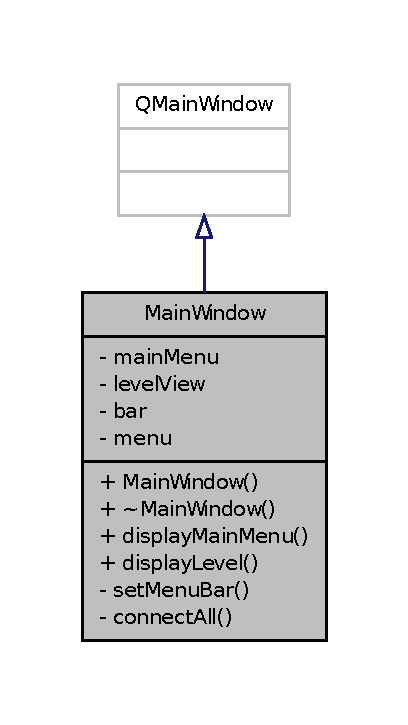
\includegraphics[width=196pt]{d1/d96/classMainWindow__inherit__graph}
\end{center}
\end{figure}


Graphe de collaboration de Main\+Window\+:\nopagebreak
\begin{figure}[H]
\begin{center}
\leavevmode
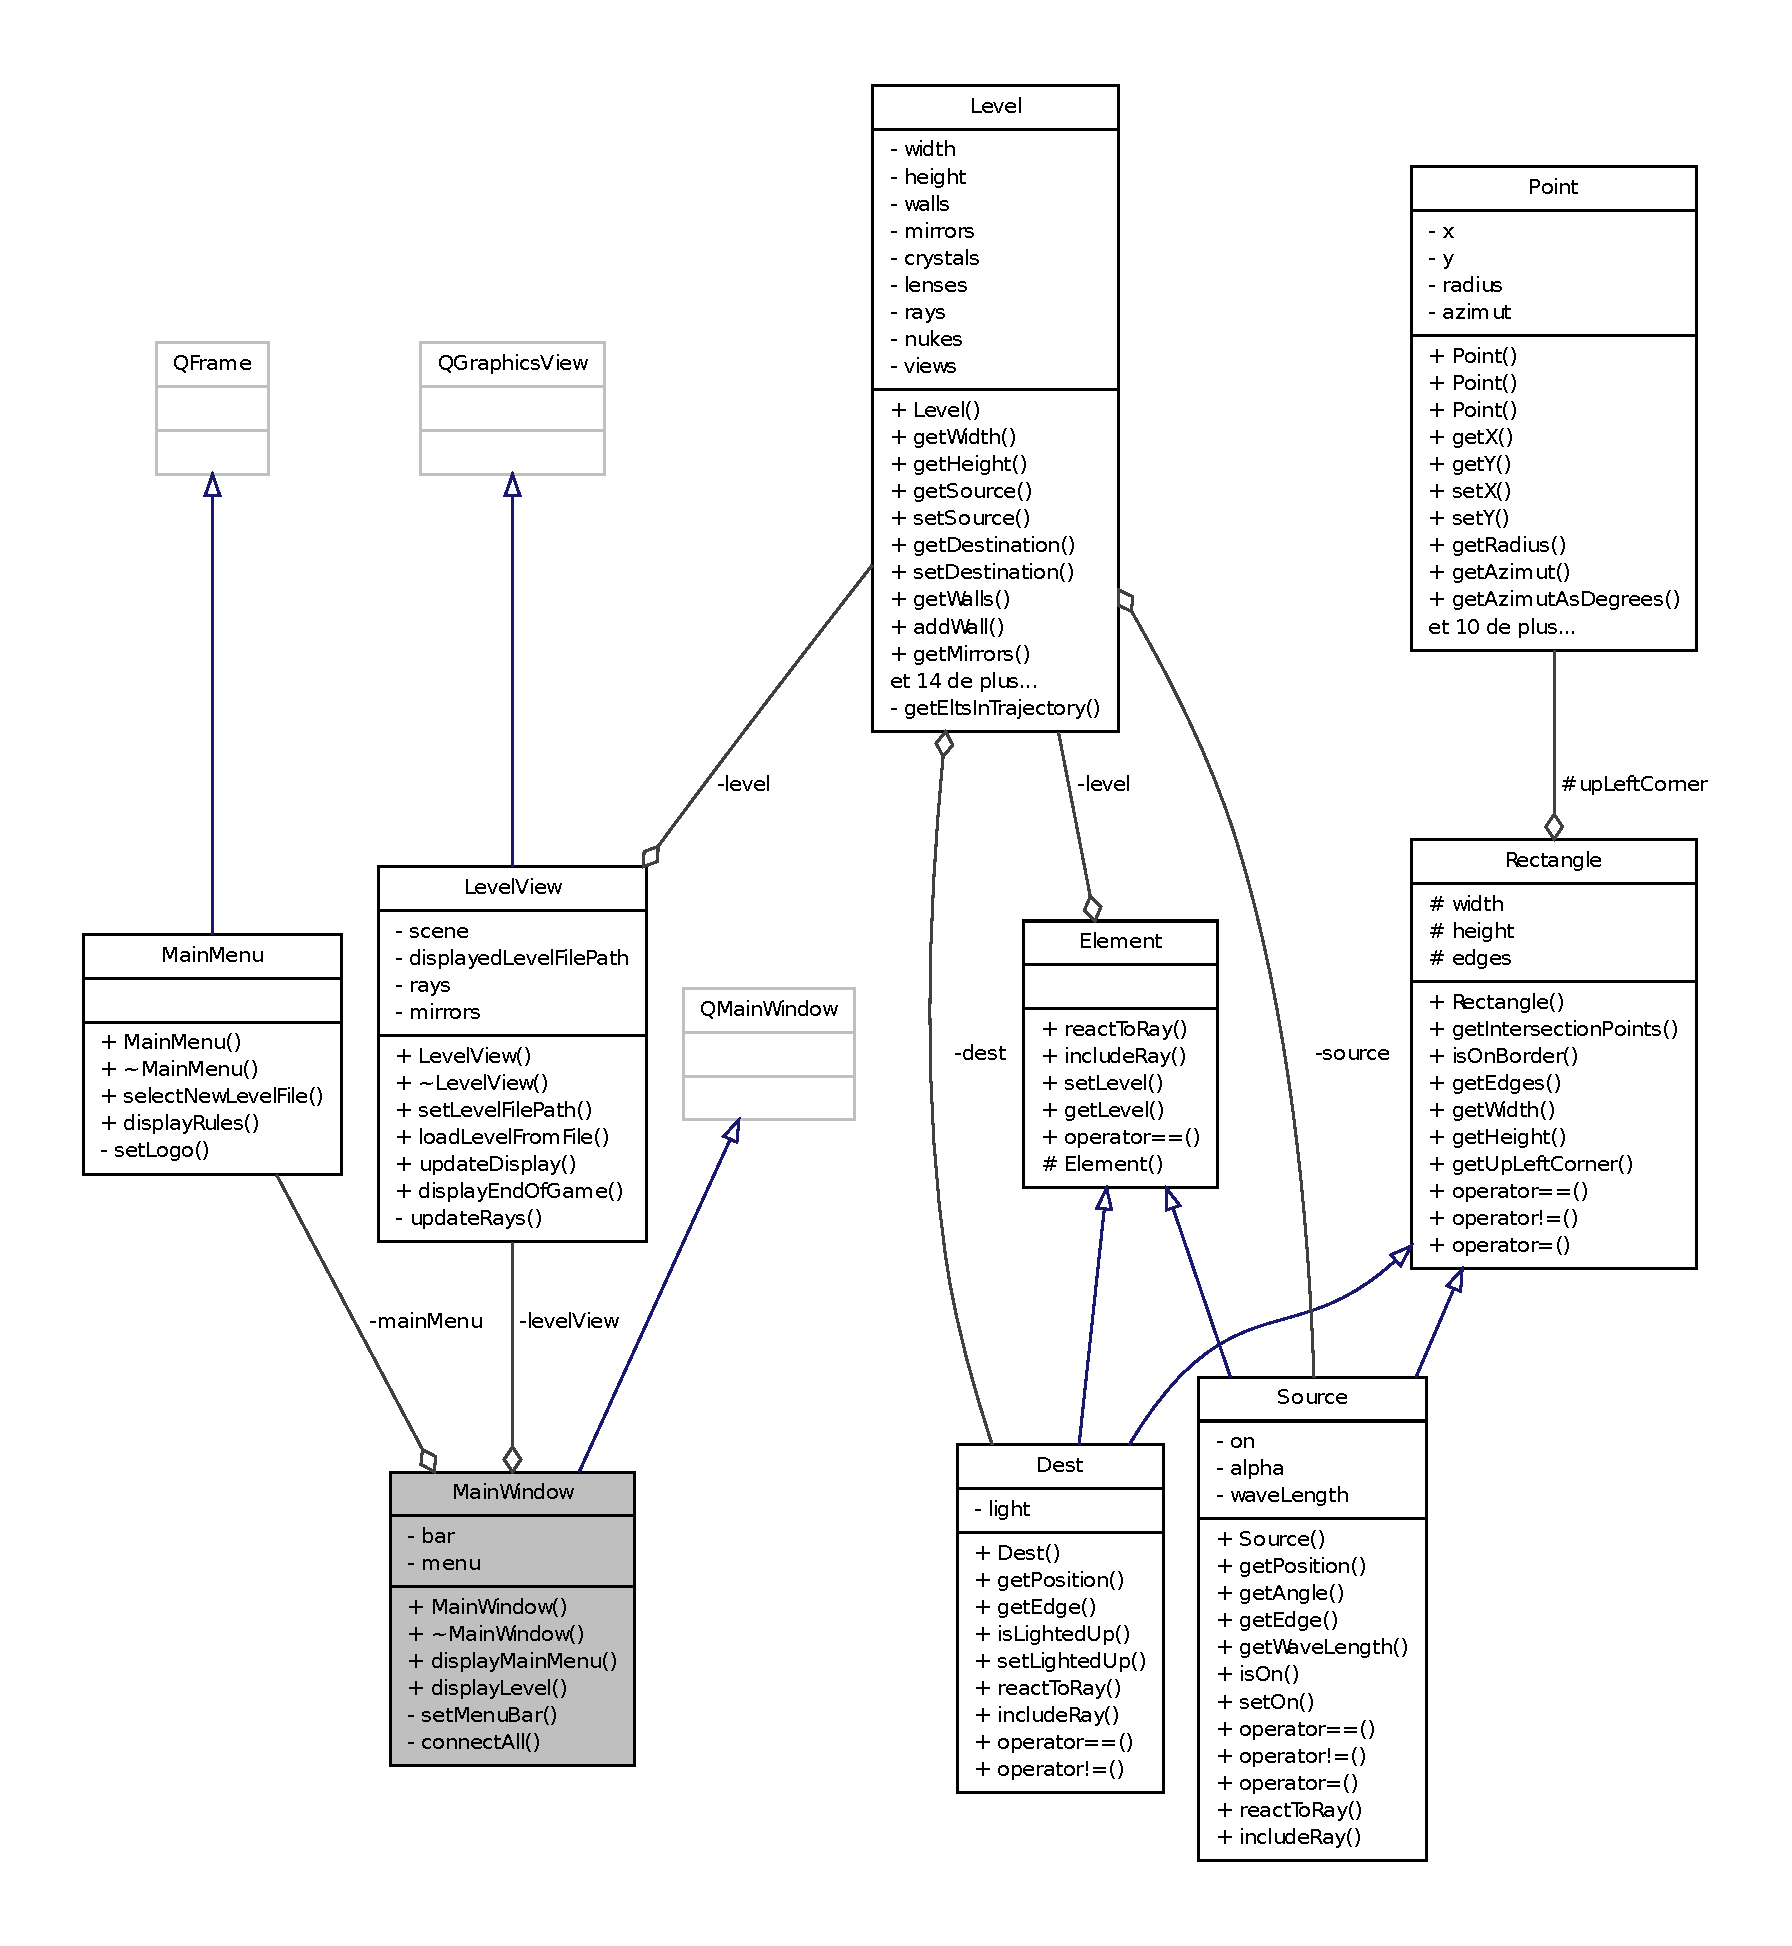
\includegraphics[width=350pt]{d2/d38/classMainWindow__coll__graph}
\end{center}
\end{figure}


\subsection{Documentation des constructeurs et destructeur}
\hypertarget{classMainWindow_a2022dfcfcd6eeba03aec9f1e6eb3ece0}{}\index{Main\+Window@{Main\+Window}!Main\+Window@{Main\+Window}}
\index{Main\+Window@{Main\+Window}!Main\+Window@{Main\+Window}}
\subsubsection[{Main\+Window(\+Q\+Widget $\ast$=0)}]{\setlength{\rightskip}{0pt plus 5cm}Main\+Window\+::\+Main\+Window (
\begin{DoxyParamCaption}
\item[{Q\+Widget $\ast$}]{ = {\ttfamily 0}}
\end{DoxyParamCaption}
)\hspace{0.3cm}{\ttfamily [explicit]}}\label{classMainWindow_a2022dfcfcd6eeba03aec9f1e6eb3ece0}


Créer une fenêtre principale du jeu. 

\hypertarget{classMainWindow_ae98d00a93bc118200eeef9f9bba1dba7}{}\index{Main\+Window@{Main\+Window}!````~Main\+Window@{$\sim$\+Main\+Window}}
\index{````~Main\+Window@{$\sim$\+Main\+Window}!Main\+Window@{Main\+Window}}
\subsubsection[{$\sim$\+Main\+Window()}]{\setlength{\rightskip}{0pt plus 5cm}Main\+Window\+::$\sim$\+Main\+Window (
\begin{DoxyParamCaption}
{}
\end{DoxyParamCaption}
)}\label{classMainWindow_ae98d00a93bc118200eeef9f9bba1dba7}


\subsection{Documentation des fonctions membres}
\hypertarget{classMainWindow_a870e523fc13b85f707e938bea8e91fd3}{}\index{Main\+Window@{Main\+Window}!connect\+All@{connect\+All}}
\index{connect\+All@{connect\+All}!Main\+Window@{Main\+Window}}
\subsubsection[{connect\+All()}]{\setlength{\rightskip}{0pt plus 5cm}void Main\+Window\+::connect\+All (
\begin{DoxyParamCaption}
{}
\end{DoxyParamCaption}
)\hspace{0.3cm}{\ttfamily [private]}}\label{classMainWindow_a870e523fc13b85f707e938bea8e91fd3}


Créer toutes les connections S\+L\+O\+T / S\+I\+G\+N\+A\+L. 

\hypertarget{classMainWindow_a0aadedf51803aeb60945aa0f809ddaa0}{}\index{Main\+Window@{Main\+Window}!display\+Level@{display\+Level}}
\index{display\+Level@{display\+Level}!Main\+Window@{Main\+Window}}
\subsubsection[{display\+Level}]{\setlength{\rightskip}{0pt plus 5cm}void Main\+Window\+::display\+Level (
\begin{DoxyParamCaption}
{}
\end{DoxyParamCaption}
)\hspace{0.3cm}{\ttfamily [slot]}}\label{classMainWindow_a0aadedf51803aeb60945aa0f809ddaa0}


Permet d\textquotesingle{}afficher le niveau. 

\hypertarget{classMainWindow_a378316f6c8670867a82a7806cfa050d8}{}\index{Main\+Window@{Main\+Window}!display\+Main\+Menu@{display\+Main\+Menu}}
\index{display\+Main\+Menu@{display\+Main\+Menu}!Main\+Window@{Main\+Window}}
\subsubsection[{display\+Main\+Menu}]{\setlength{\rightskip}{0pt plus 5cm}void Main\+Window\+::display\+Main\+Menu (
\begin{DoxyParamCaption}
{}
\end{DoxyParamCaption}
)\hspace{0.3cm}{\ttfamily [slot]}}\label{classMainWindow_a378316f6c8670867a82a7806cfa050d8}


Permet d\textquotesingle{}afficher le menu principal du jeu. 

\hypertarget{classMainWindow_a306206f30c08b874636f48ed79192e86}{}\index{Main\+Window@{Main\+Window}!set\+Menu\+Bar@{set\+Menu\+Bar}}
\index{set\+Menu\+Bar@{set\+Menu\+Bar}!Main\+Window@{Main\+Window}}
\subsubsection[{set\+Menu\+Bar()}]{\setlength{\rightskip}{0pt plus 5cm}void Main\+Window\+::set\+Menu\+Bar (
\begin{DoxyParamCaption}
{}
\end{DoxyParamCaption}
)\hspace{0.3cm}{\ttfamily [private]}}\label{classMainWindow_a306206f30c08b874636f48ed79192e86}


Configure la bar de menu. 



\subsection{Documentation des données membres}
\hypertarget{classMainWindow_af362dbdd2f874d380a02700ce5dbe42c}{}\index{Main\+Window@{Main\+Window}!bar@{bar}}
\index{bar@{bar}!Main\+Window@{Main\+Window}}
\subsubsection[{bar}]{\setlength{\rightskip}{0pt plus 5cm}Q\+Menu\+Bar$\ast$ Main\+Window\+::bar\hspace{0.3cm}{\ttfamily [private]}}\label{classMainWindow_af362dbdd2f874d380a02700ce5dbe42c}


La bar de menu du jeu. 



Définition à la ligne 34 du fichier mainwindow.\+hpp.

\hypertarget{classMainWindow_a62681b0c049afcba55ffbd5e5f470ca3}{}\index{Main\+Window@{Main\+Window}!level\+View@{level\+View}}
\index{level\+View@{level\+View}!Main\+Window@{Main\+Window}}
\subsubsection[{level\+View}]{\setlength{\rightskip}{0pt plus 5cm}{\bf Level\+View}$\ast$ Main\+Window\+::level\+View\hspace{0.3cm}{\ttfamily [private]}}\label{classMainWindow_a62681b0c049afcba55ffbd5e5f470ca3}


La vue de la partie qui est lancée. 



Définition à la ligne 29 du fichier mainwindow.\+hpp.

\hypertarget{classMainWindow_acff78d8b40fc6a64c3503e9fcf120df2}{}\index{Main\+Window@{Main\+Window}!main\+Menu@{main\+Menu}}
\index{main\+Menu@{main\+Menu}!Main\+Window@{Main\+Window}}
\subsubsection[{main\+Menu}]{\setlength{\rightskip}{0pt plus 5cm}{\bf Main\+Menu}$\ast$ Main\+Window\+::main\+Menu\hspace{0.3cm}{\ttfamily [private]}}\label{classMainWindow_acff78d8b40fc6a64c3503e9fcf120df2}


Le menu de sélection de niveau du jeu. 



Définition à la ligne 24 du fichier mainwindow.\+hpp.

\hypertarget{classMainWindow_a42e15f7cdb120e053ef72a06d11d73f6}{}\index{Main\+Window@{Main\+Window}!menu@{menu}}
\index{menu@{menu}!Main\+Window@{Main\+Window}}
\subsubsection[{menu}]{\setlength{\rightskip}{0pt plus 5cm}Q\+Menu$\ast$ Main\+Window\+::menu\hspace{0.3cm}{\ttfamily [private]}}\label{classMainWindow_a42e15f7cdb120e053ef72a06d11d73f6}


Le menu principal du jeu. 



Définition à la ligne 39 du fichier mainwindow.\+hpp.



La documentation de cette classe a été générée à partir du fichier suivant \+:\begin{DoxyCompactItemize}
\item 
view/windows/\hyperlink{mainwindow_8hpp}{mainwindow.\+hpp}\end{DoxyCompactItemize}

\hypertarget{classMirror}{}\section{Référence de la classe Mirror}
\label{classMirror}\index{Mirror@{Mirror}}


Cette classe modélise les miroirs utilisés dans le jeu.  




{\ttfamily \#include $<$mirror.\+hpp$>$}

\subsection*{Fonctions membres publiques}
\begin{DoxyCompactItemize}
\item 
\hyperlink{classMirror_aad395af8bb0ef4c68259cc3c694fe663}{Mirror} (const \hyperlink{classPoint}{Point} \&, int, int, double)
\begin{DoxyCompactList}\small\item\em Instancie un miroir en une position donnée, d\textquotesingle{}une certaine longueur et orienté d\textquotesingle{}un certain angle. \end{DoxyCompactList}\item 
\hyperlink{classMirror_afe425460546bb3849fc6a943973e59ef}{Mirror} (const \hyperlink{classPoint}{Point} \&, int, int, double, \hyperlink{classPoint}{Point}, \hyperlink{classPoint}{Point}, double, double)
\begin{DoxyCompactList}\small\item\em Instancie un miroir en une position donnée, d\textquotesingle{}une certaine longueur et orienté d\textquotesingle{}un certain angle. \end{DoxyCompactList}\item 
const \hyperlink{classPoint}{Point} \& \hyperlink{classMirror_a2019420aed1cd71cc5b70ea7f9e0029e}{get\+Pivot} () const 
\begin{DoxyCompactList}\small\item\em Retourne la position du pivot du miroir. \end{DoxyCompactList}\item 
int \hyperlink{classMirror_a10044b17327d12c0fb05b086e98ae4f4}{get\+Length} () const 
\begin{DoxyCompactList}\small\item\em Retourne la longueur du miroir. \end{DoxyCompactList}\item 
int \hyperlink{classMirror_a5f539d8343f70ec68eaee6fd472049ae}{get\+X\+Pad} () const 
\begin{DoxyCompactList}\small\item\em Retourne le décalage du pivot par rapport au bord gauche du miroir. \end{DoxyCompactList}\item 
double \hyperlink{classMirror_a6bdf519d0a2135536c78d38582d277ea}{get\+Angle} () const 
\begin{DoxyCompactList}\small\item\em Retourne l\textquotesingle{}inclinaison du miroir. \end{DoxyCompactList}\item 
double \hyperlink{classMirror_a1aecd262fdf636697e6027da60685bb9}{get\+Min\+Angle} () const 
\begin{DoxyCompactList}\small\item\em Retourne l\textquotesingle{}inclinaison minimum du miroir. \end{DoxyCompactList}\item 
double \hyperlink{classMirror_aedb5e8c9ddad54164921fdf75f4270d9}{get\+Max\+Angle} () const 
\begin{DoxyCompactList}\small\item\em Retourne l\textquotesingle{}inclinaison minimum du miroir. \end{DoxyCompactList}\item 
\hyperlink{classPoint}{Point} \hyperlink{classMirror_a589b4be142b61fcc247ce61bd8ec5d47}{get\+Min\+Pivot} () const 
\begin{DoxyCompactList}\small\item\em Retourne la position minimum du miroir. \end{DoxyCompactList}\item 
\hyperlink{classPoint}{Point} \hyperlink{classMirror_a2b1383e76cc709b4b51f10492d9ed1ad}{get\+Max\+Pivot} () const 
\begin{DoxyCompactList}\small\item\em Retourne la position maximum du miroir. \end{DoxyCompactList}\item 
bool \hyperlink{classMirror_a83f8934245fe330510b031a19fa77fbe}{set\+Pivot} (const \hyperlink{classPoint}{Point} \&)
\begin{DoxyCompactList}\small\item\em Déplace le miroir en la position donnée, si celle-\/ci est autorisée. \end{DoxyCompactList}\item 
bool \hyperlink{classMirror_aa5c28cf6d8a88d11f06b4140389c2a06}{set\+Angle} (double)
\begin{DoxyCompactList}\small\item\em Pivote le miroir sur un angle donné, si celui-\/ci est autorisé. \end{DoxyCompactList}\item 
bool \hyperlink{classMirror_a35dd50199a1bb8f2a0dea49259df6e95}{rotate} (double)
\begin{DoxyCompactList}\small\item\em Permet d\textquotesingle{}{\bfseries essayer} d\textquotesingle{}effectuer une rotation du miroir courant. \end{DoxyCompactList}\item 
bool \hyperlink{classMirror_ac9c58d670d8c84b41135c07fedd0b502}{translate} (const double, const double)
\begin{DoxyCompactList}\small\item\em Permet de déplacer le miroir dans le plan en lui donnant un abscisse et une ordonnée de translation. \end{DoxyCompactList}\item 
\hyperlink{classPoint}{Point} \hyperlink{classMirror_aad24b622e2f9c18691ec70a1bbdadbcf}{get\+Start} () const 
\begin{DoxyCompactList}\small\item\em Retourne le point de départ du segment de droite représentant le miroir. \end{DoxyCompactList}\item 
\hyperlink{classPoint}{Point} \hyperlink{classMirror_ae9ba03e1a3d35a85f8b55ec6ea2a7462}{get\+End} () const 
\begin{DoxyCompactList}\small\item\em Retourne le point d\textquotesingle{} arrivé du segment de droite représentant le miroir. \end{DoxyCompactList}\item 
void \hyperlink{classMirror_a4d3fe38f3bbe5b546384ef0fb81f16c4}{get\+Bounds} (\hyperlink{classPoint}{Point} $\ast$, \hyperlink{classPoint}{Point} $\ast$) const 
\begin{DoxyCompactList}\small\item\em Permet d\textquotesingle{}obtenir le point de départ et d\textquotesingle{}arrivé du segment de droite représentant le miroir; pour éviter de retourner un conteneur de points, ceux-\/ci sont passés en entrée sortie des paramètres. \end{DoxyCompactList}\item 
bool \hyperlink{classMirror_aa4fc01092dae3dab55dd2e74af41f429}{check\+Angle\+Range} (double) const 
\begin{DoxyCompactList}\small\item\em Retoune vrai si le miroir peut être pivoté sur l\textquotesingle{}angle donné, retourne faux sinon. \end{DoxyCompactList}\item 
bool \hyperlink{classMirror_a52f096a72ba715cba18d5d3d79d507f4}{check\+Pivot\+Range} (const \hyperlink{classPoint}{Point} \&) const 
\begin{DoxyCompactList}\small\item\em Retoune vrai si le miroir peut être déplacé en la position donnée, retourne faux sinon. \end{DoxyCompactList}\item 
void \hyperlink{classMirror_a149fb6af1dcdcffd685b21019f189c72}{react\+To\+Ray} (\hyperlink{classRay}{Ray})
\begin{DoxyCompactList}\small\item\em Réaction à l\textquotesingle{}exposition d\textquotesingle{}un rayon; celui-\/ci est réfléchi selon le principe naturel de la réflexion de la lumière dans l\textquotesingle{}air. \end{DoxyCompactList}\item 
\hyperlink{classPoint}{Point} $\ast$ \hyperlink{classMirror_af9b8d54ae559b388cb04df6f8d391f47}{include\+Ray} (const \hyperlink{classRay}{Ray} \&) const 
\begin{DoxyCompactList}\small\item\em Renseigne si le miroir est dans la trajectoire du rayon. \end{DoxyCompactList}\item 
bool \hyperlink{classMirror_aca852b6cf22bec88a402d3b7e7c78ca9}{operator==} (const \hyperlink{classMirror}{Mirror} \&) const 
\begin{DoxyCompactList}\small\item\em Permet de savoir si deux miroirs sont les même. \end{DoxyCompactList}\item 
bool \hyperlink{classMirror_a0538deb5f7234df6cf635e3836d6dfae}{operator!=} (const \hyperlink{classMirror}{Mirror} \&) const 
\begin{DoxyCompactList}\small\item\em Permet de savoir si deux miroirs sont différents. \end{DoxyCompactList}\end{DoxyCompactItemize}
\subsection*{Attributs privés}
\begin{DoxyCompactItemize}
\item 
\hyperlink{classPoint}{Point} \hyperlink{classMirror_aeec9a930fcc8f87373a5ca5c403edc53}{pivot}
\begin{DoxyCompactList}\small\item\em Le point de pivot du miroir autour du quel celui-\/ci peut effectuer une rotation. \end{DoxyCompactList}\item 
int \hyperlink{classMirror_a03f7e5469eaa52fa2090542182f99fbd}{length}
\begin{DoxyCompactList}\small\item\em La longueur totale du miroir. \end{DoxyCompactList}\item 
int \hyperlink{classMirror_aef41f122c76a825af7d12eaddf6ff1ea}{xpad}
\begin{DoxyCompactList}\small\item\em La longueur séparant le point de pivot d\textquotesingle{}un point extrême du miroir. \end{DoxyCompactList}\item 
double \hyperlink{classMirror_a797115030b6a7bded6bab18a080e30c6}{x\+Min}
\begin{DoxyCompactList}\small\item\em Limite minimale d\textquotesingle{}abscisse où peut se situer le pivot du miroir. \end{DoxyCompactList}\item 
double \hyperlink{classMirror_ab0e8322594aeb39432b4696d67e3ba6d}{x\+Max}
\begin{DoxyCompactList}\small\item\em Limite maximale d\textquotesingle{}abscisse où peut se situer le pivot du miroir. \end{DoxyCompactList}\item 
double \hyperlink{classMirror_a4b18a9326165e36b1ae05604b34ce758}{y\+Min}
\begin{DoxyCompactList}\small\item\em Limite minimale d\textquotesingle{}ordonnée où peut se situer le pivot du miroir. \end{DoxyCompactList}\item 
double \hyperlink{classMirror_a2e76c506f910e388db245355ab17ce3a}{y\+Max}
\begin{DoxyCompactList}\small\item\em Limite maximale d\textquotesingle{}ordonnée où peut se situer le pivot du miroir. \end{DoxyCompactList}\item 
double \hyperlink{classMirror_a28ecd988b42db315b57fc8d9b23ebd86}{alpha}
\begin{DoxyCompactList}\small\item\em L\textquotesingle{}angle actuel de rotation du miroir. \end{DoxyCompactList}\item 
double \hyperlink{classMirror_ac42fb9a193abfb984ca27bbad2564ff9}{alpha\+Min}
\begin{DoxyCompactList}\small\item\em L\textquotesingle{}angle minimum dans lequel peut se trouver le miroir. \end{DoxyCompactList}\item 
double \hyperlink{classMirror_acc41ebc589e76d723bff02eea9ddfee3}{alpha\+Max}
\begin{DoxyCompactList}\small\item\em L\textquotesingle{}angle maximum dans lequel peut se trouver le miroir. \end{DoxyCompactList}\end{DoxyCompactItemize}
\subsection*{Membres hérités additionnels}


\subsection{Description détaillée}
Cette classe modélise les miroirs utilisés dans le jeu. 

Un miroir est un segment de droite dont la propriété est de réfléchir la lumière d\textquotesingle{}un seul côté uniquement. Si un rayon lumineux touche un miroir du côté non réfléchissant, le miroir se comporte comme un mur. Les miroirs sont capables d\textquotesingle{}être déplacés et pivotés dans une certaine limite. 

Définition à la ligne 21 du fichier mirror.\+hpp.



Graphe d\textquotesingle{}héritage de Mirror\+:\nopagebreak
\begin{figure}[H]
\begin{center}
\leavevmode
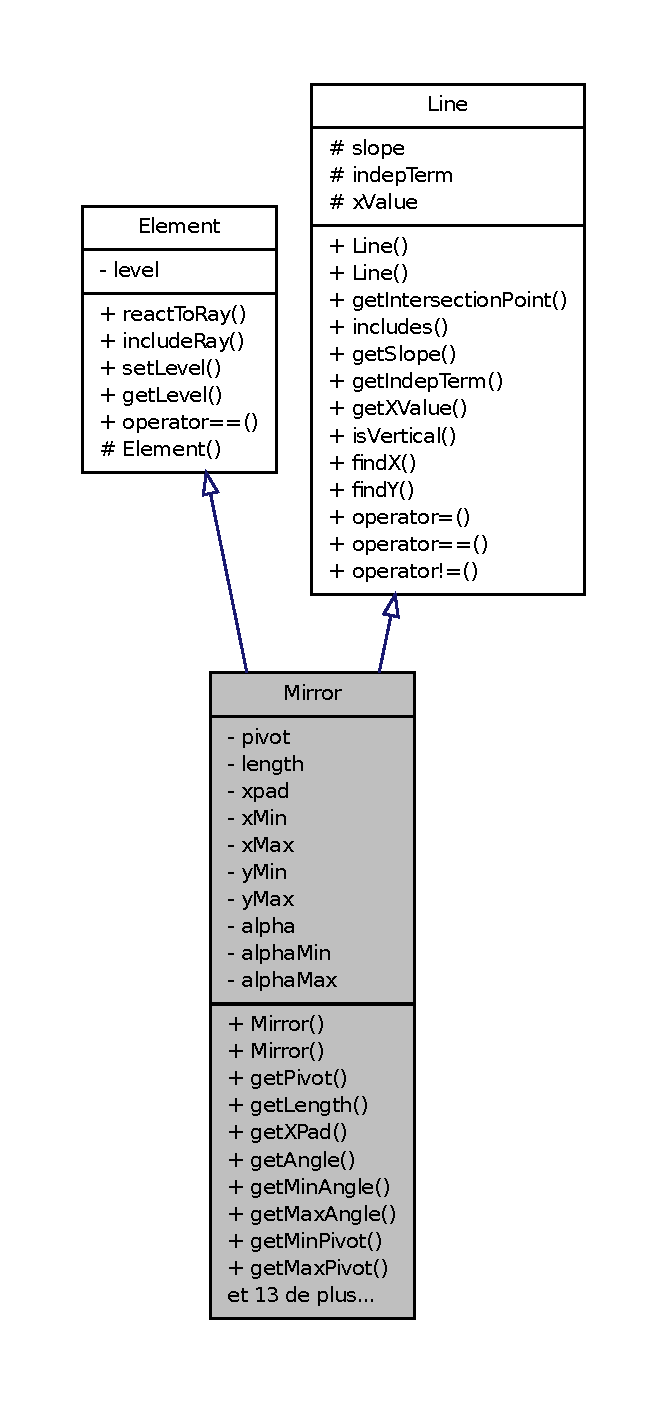
\includegraphics[height=550pt]{d8/d7d/classMirror__inherit__graph}
\end{center}
\end{figure}


Graphe de collaboration de Mirror\+:\nopagebreak
\begin{figure}[H]
\begin{center}
\leavevmode
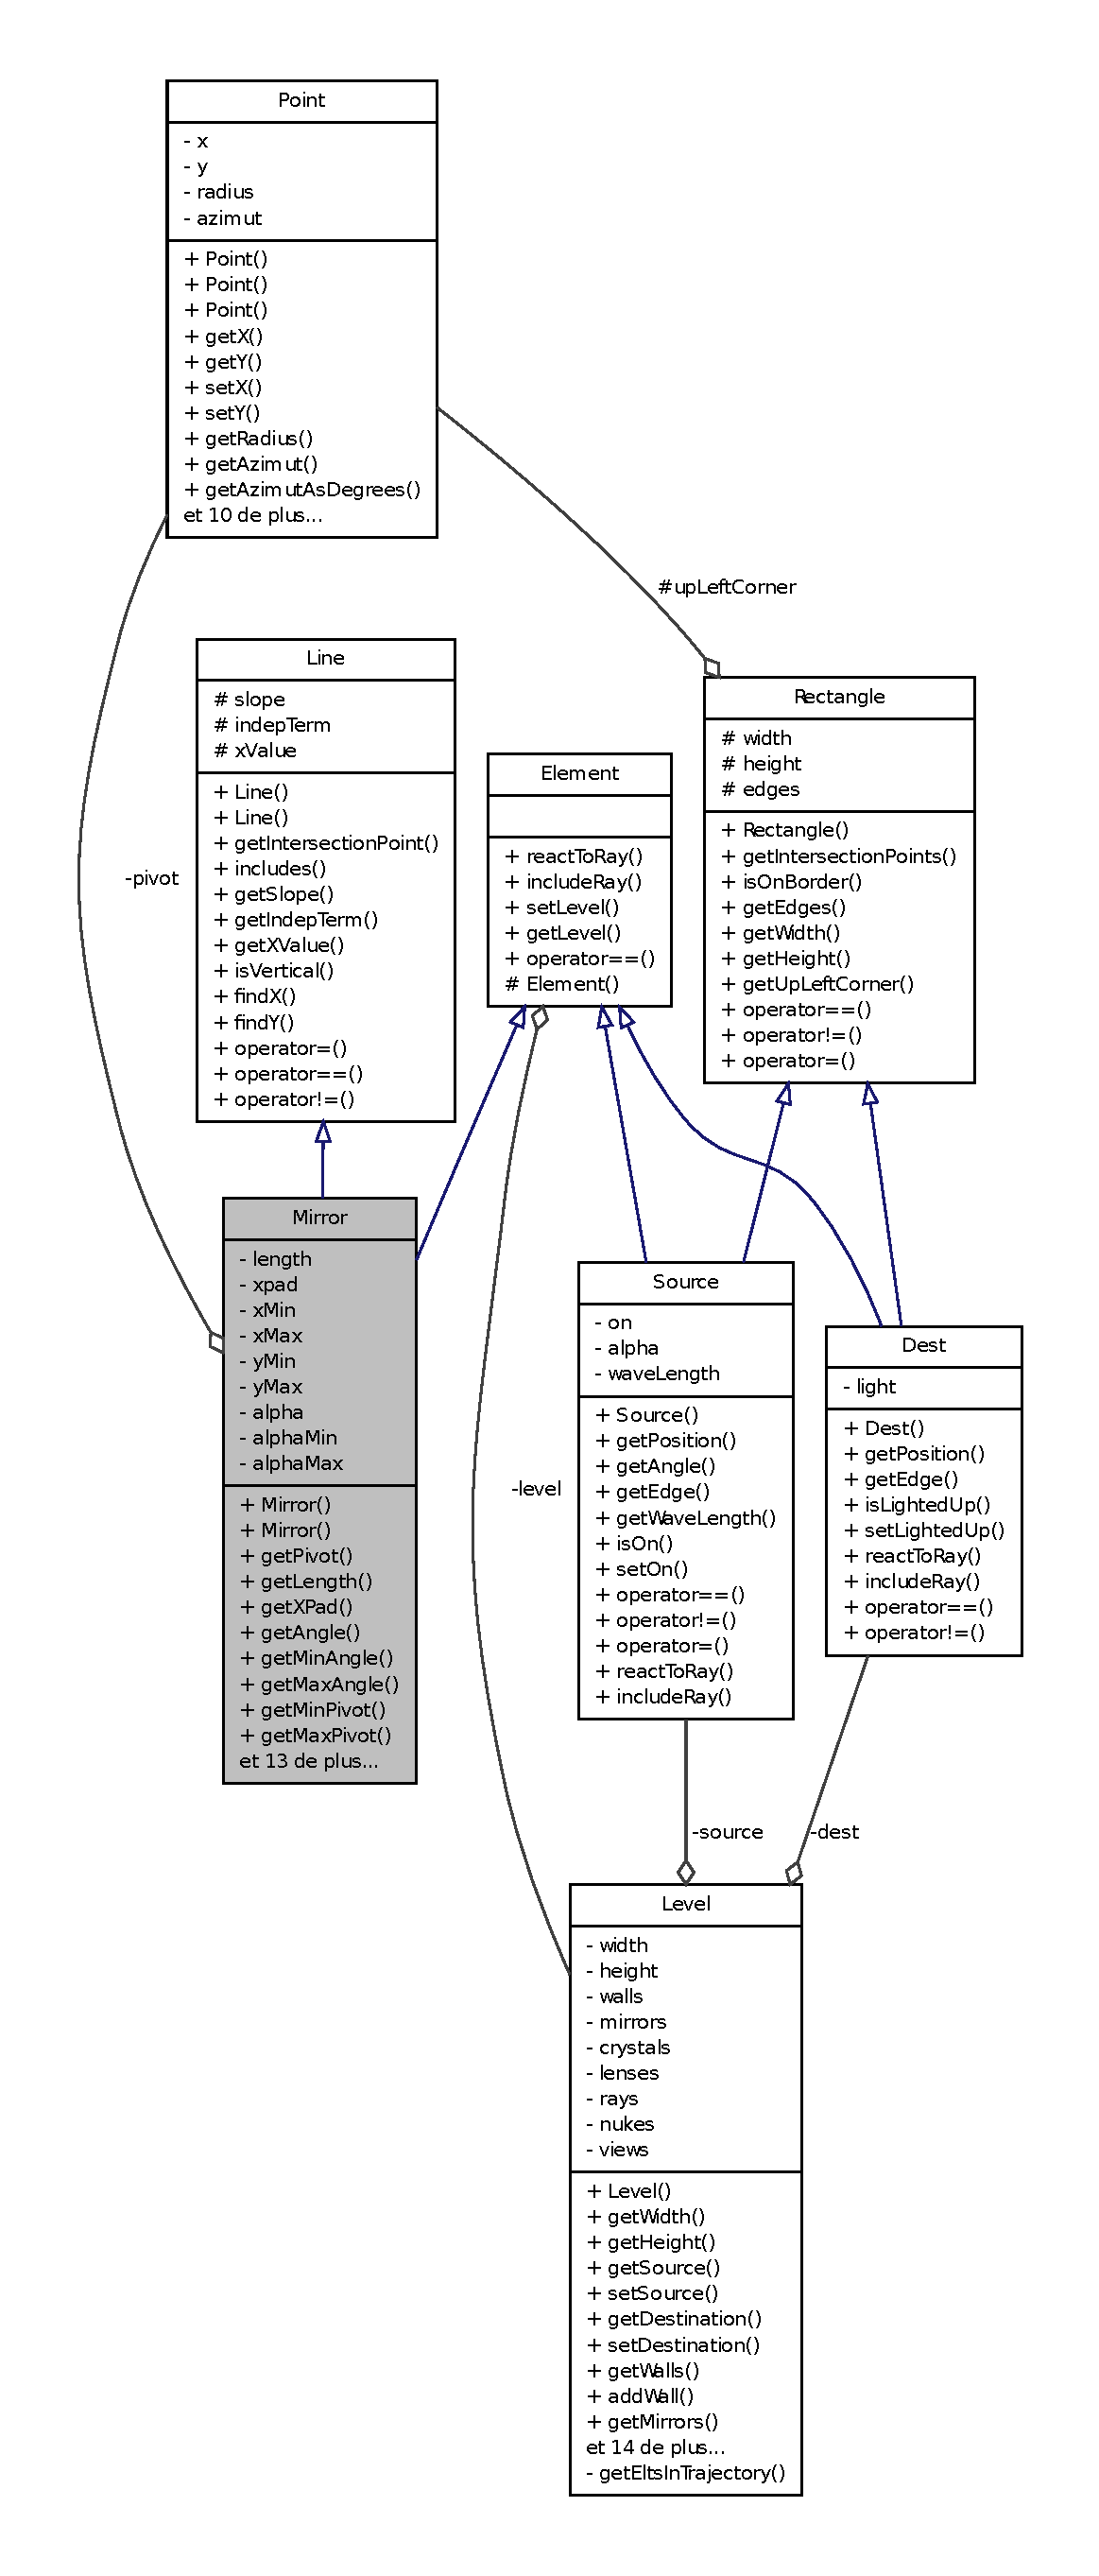
\includegraphics[height=550pt]{dc/d9b/classMirror__coll__graph}
\end{center}
\end{figure}


\subsection{Documentation des constructeurs et destructeur}
\hypertarget{classMirror_aad395af8bb0ef4c68259cc3c694fe663}{}\index{Mirror@{Mirror}!Mirror@{Mirror}}
\index{Mirror@{Mirror}!Mirror@{Mirror}}
\subsubsection[{Mirror(const Point \&, int, int, double)}]{\setlength{\rightskip}{0pt plus 5cm}Mirror\+::\+Mirror (
\begin{DoxyParamCaption}
\item[{const {\bf Point} \&}]{, }
\item[{int}]{, }
\item[{int}]{, }
\item[{double}]{}
\end{DoxyParamCaption}
)}\label{classMirror_aad395af8bb0ef4c68259cc3c694fe663}


Instancie un miroir en une position donnée, d\textquotesingle{}une certaine longueur et orienté d\textquotesingle{}un certain angle. 

Comme dans ce constructeur les limites de déplacement et de rotation du miroir ne sont pas définies, ce miroir peut se déplacer et pivoter librement.


\begin{DoxyParams}{Paramètres}
{\em pivot} & La position du pivot du miroir. \\
\hline
{\em xpad} & Le décalage du pivot par rapport au bord gauche du miroir. \\
\hline
{\em length} & La longueur du miroir. \\
\hline
{\em alpha} & L\textquotesingle{}angle d\textquotesingle{}inclinaison du miroir. \\
\hline
\end{DoxyParams}
\hypertarget{classMirror_afe425460546bb3849fc6a943973e59ef}{}\index{Mirror@{Mirror}!Mirror@{Mirror}}
\index{Mirror@{Mirror}!Mirror@{Mirror}}
\subsubsection[{Mirror(const Point \&, int, int, double, Point, Point, double, double)}]{\setlength{\rightskip}{0pt plus 5cm}Mirror\+::\+Mirror (
\begin{DoxyParamCaption}
\item[{const {\bf Point} \&}]{, }
\item[{int}]{, }
\item[{int}]{, }
\item[{double}]{, }
\item[{{\bf Point}}]{, }
\item[{{\bf Point}}]{, }
\item[{double}]{, }
\item[{double}]{}
\end{DoxyParamCaption}
)}\label{classMirror_afe425460546bb3849fc6a943973e59ef}


Instancie un miroir en une position donnée, d\textquotesingle{}une certaine longueur et orienté d\textquotesingle{}un certain angle. 

Ce constructeur permet également aux miroirs de pivoter dans une certaine limite. Si l\textquotesingle{}intervalle de limite de déplacement (e.\+g., sur les abscisses) \mbox{[}a,b\mbox{]} est tel que si \+: 
\begin{DoxyItemize}
\item a = b, le miroir ne peut être déplacé sur l\textquotesingle{}axe considéré 
\item a $<$ b, le miroir pivote dans le sens horloger 
\item a = b le miroir ne peut pas pivoter 
\item a $>$ b, le miroir pivote dans le sens anti-\/horloger 
\end{DoxyItemize}


\begin{DoxyParams}{Paramètres}
{\em pivot} & La position du pivot du miroir. \\
\hline
{\em xpad} & Le décalage du pivot par rapport au bord gauche du miroir. \\
\hline
{\em length} & La longueur du miroir. \\
\hline
{\em alpha} & L\textquotesingle{}angle d\textquotesingle{}inclinaison du miroir. \\
\hline
{\em point\+Min} & Le point de coordonnées minimum. \\
\hline
{\em point\+Max} & Le point de coordonnées maximum. \\
\hline
{\em alpha\+Min} & L\textquotesingle{}angle d\textquotesingle{}inclinaison minimum du miroir (en radian). \\
\hline
{\em alpha\+Max} & L\textquotesingle{}angle d\textquotesingle{}inclinaison maximum du miroir (en radian). \\
\hline
\end{DoxyParams}


\subsection{Documentation des fonctions membres}
\hypertarget{classMirror_aa4fc01092dae3dab55dd2e74af41f429}{}\index{Mirror@{Mirror}!check\+Angle\+Range@{check\+Angle\+Range}}
\index{check\+Angle\+Range@{check\+Angle\+Range}!Mirror@{Mirror}}
\subsubsection[{check\+Angle\+Range(double) const }]{\setlength{\rightskip}{0pt plus 5cm}bool Mirror\+::check\+Angle\+Range (
\begin{DoxyParamCaption}
\item[{double}]{}
\end{DoxyParamCaption}
) const}\label{classMirror_aa4fc01092dae3dab55dd2e74af41f429}


Retoune vrai si le miroir peut être pivoté sur l\textquotesingle{}angle donné, retourne faux sinon. 

\begin{DoxyReturn}{Renvoie}
{\ttfamily true} si le miroir peut être pivoté sur l\textquotesingle{}angle donné, retourne faux sinon. 
\end{DoxyReturn}
\hypertarget{classMirror_a52f096a72ba715cba18d5d3d79d507f4}{}\index{Mirror@{Mirror}!check\+Pivot\+Range@{check\+Pivot\+Range}}
\index{check\+Pivot\+Range@{check\+Pivot\+Range}!Mirror@{Mirror}}
\subsubsection[{check\+Pivot\+Range(const Point \&) const }]{\setlength{\rightskip}{0pt plus 5cm}bool Mirror\+::check\+Pivot\+Range (
\begin{DoxyParamCaption}
\item[{const {\bf Point} \&}]{}
\end{DoxyParamCaption}
) const}\label{classMirror_a52f096a72ba715cba18d5d3d79d507f4}


Retoune vrai si le miroir peut être déplacé en la position donnée, retourne faux sinon. 

\begin{DoxyReturn}{Renvoie}
{\ttfamily true} si le miroir peut être déplacé en la position donnée, retourne faux sinon. 
\end{DoxyReturn}
\hypertarget{classMirror_a6bdf519d0a2135536c78d38582d277ea}{}\index{Mirror@{Mirror}!get\+Angle@{get\+Angle}}
\index{get\+Angle@{get\+Angle}!Mirror@{Mirror}}
\subsubsection[{get\+Angle() const }]{\setlength{\rightskip}{0pt plus 5cm}double Mirror\+::get\+Angle (
\begin{DoxyParamCaption}
{}
\end{DoxyParamCaption}
) const\hspace{0.3cm}{\ttfamily [inline]}}\label{classMirror_a6bdf519d0a2135536c78d38582d277ea}


Retourne l\textquotesingle{}inclinaison du miroir. 

\begin{DoxyReturn}{Renvoie}
l\textquotesingle{}inclinaison du miroir. 
\end{DoxyReturn}


Définition à la ligne 338 du fichier mirror.\+hpp.



Références alpha.


\begin{DoxyCode}
339 \{
340     \textcolor{keywordflow}{return} this->\hyperlink{classMirror_a28ecd988b42db315b57fc8d9b23ebd86}{alpha};
341 \}
\end{DoxyCode}
\hypertarget{classMirror_a4d3fe38f3bbe5b546384ef0fb81f16c4}{}\index{Mirror@{Mirror}!get\+Bounds@{get\+Bounds}}
\index{get\+Bounds@{get\+Bounds}!Mirror@{Mirror}}
\subsubsection[{get\+Bounds(\+Point $\ast$, Point $\ast$) const }]{\setlength{\rightskip}{0pt plus 5cm}void Mirror\+::get\+Bounds (
\begin{DoxyParamCaption}
\item[{{\bf Point} $\ast$}]{, }
\item[{{\bf Point} $\ast$}]{}
\end{DoxyParamCaption}
) const}\label{classMirror_a4d3fe38f3bbe5b546384ef0fb81f16c4}


Permet d\textquotesingle{}obtenir le point de départ et d\textquotesingle{}arrivé du segment de droite représentant le miroir; pour éviter de retourner un conteneur de points, ceux-\/ci sont passés en entrée sortie des paramètres. 

\hypertarget{classMirror_ae9ba03e1a3d35a85f8b55ec6ea2a7462}{}\index{Mirror@{Mirror}!get\+End@{get\+End}}
\index{get\+End@{get\+End}!Mirror@{Mirror}}
\subsubsection[{get\+End() const }]{\setlength{\rightskip}{0pt plus 5cm}{\bf Point} Mirror\+::get\+End (
\begin{DoxyParamCaption}
{}
\end{DoxyParamCaption}
) const}\label{classMirror_ae9ba03e1a3d35a85f8b55ec6ea2a7462}


Retourne le point d\textquotesingle{} arrivé du segment de droite représentant le miroir. 

\begin{DoxyReturn}{Renvoie}
Le point d\textquotesingle{}arrivé du segment de droite représentant le miroir. 
\end{DoxyReturn}
\hypertarget{classMirror_a10044b17327d12c0fb05b086e98ae4f4}{}\index{Mirror@{Mirror}!get\+Length@{get\+Length}}
\index{get\+Length@{get\+Length}!Mirror@{Mirror}}
\subsubsection[{get\+Length() const }]{\setlength{\rightskip}{0pt plus 5cm}int Mirror\+::get\+Length (
\begin{DoxyParamCaption}
{}
\end{DoxyParamCaption}
) const\hspace{0.3cm}{\ttfamily [inline]}}\label{classMirror_a10044b17327d12c0fb05b086e98ae4f4}


Retourne la longueur du miroir. 

\begin{DoxyReturn}{Renvoie}
La longueur du miroir. 
\end{DoxyReturn}


Définition à la ligne 328 du fichier mirror.\+hpp.



Références length.


\begin{DoxyCode}
329 \{
330     \textcolor{keywordflow}{return} this->\hyperlink{classMirror_a03f7e5469eaa52fa2090542182f99fbd}{length};
331 \}
\end{DoxyCode}
\hypertarget{classMirror_aedb5e8c9ddad54164921fdf75f4270d9}{}\index{Mirror@{Mirror}!get\+Max\+Angle@{get\+Max\+Angle}}
\index{get\+Max\+Angle@{get\+Max\+Angle}!Mirror@{Mirror}}
\subsubsection[{get\+Max\+Angle() const }]{\setlength{\rightskip}{0pt plus 5cm}double Mirror\+::get\+Max\+Angle (
\begin{DoxyParamCaption}
{}
\end{DoxyParamCaption}
) const\hspace{0.3cm}{\ttfamily [inline]}}\label{classMirror_aedb5e8c9ddad54164921fdf75f4270d9}


Retourne l\textquotesingle{}inclinaison minimum du miroir. 

Si l\textquotesingle{}intervalle de limite d\textquotesingle{}inclinaison \mbox{[}a,b\mbox{]} est tel que \+: 
\begin{DoxyItemize}
\item a $<$ b, le miroir pivote dans le sens horloger 
\item a = b, le miroir ne peut pas pivoter 
\item a $>$ b, le miroir pivote dans le sens anti-\/horloger 
\item Si a = b = 0, le miroir peut être pivoté librement 
\end{DoxyItemize}

\begin{DoxyReturn}{Renvoie}
l\textquotesingle{}inclinaison maximum du miroir en radian. 
\end{DoxyReturn}


Définition à la ligne 348 du fichier mirror.\+hpp.



Références alpha\+Max.


\begin{DoxyCode}
349 \{
350     \textcolor{keywordflow}{return} this->\hyperlink{classMirror_acc41ebc589e76d723bff02eea9ddfee3}{alphaMax};
351 \}
\end{DoxyCode}
\hypertarget{classMirror_a2b1383e76cc709b4b51f10492d9ed1ad}{}\index{Mirror@{Mirror}!get\+Max\+Pivot@{get\+Max\+Pivot}}
\index{get\+Max\+Pivot@{get\+Max\+Pivot}!Mirror@{Mirror}}
\subsubsection[{get\+Max\+Pivot() const }]{\setlength{\rightskip}{0pt plus 5cm}{\bf Point} Mirror\+::get\+Max\+Pivot (
\begin{DoxyParamCaption}
{}
\end{DoxyParamCaption}
) const}\label{classMirror_a2b1383e76cc709b4b51f10492d9ed1ad}


Retourne la position maximum du miroir. 

Si l\textquotesingle{}intervalle de limite de déplacement (e.\+g., sur les abscisses) \mbox{[}a,b\mbox{]} est tel que a = b, le miroir ne peut être déplacé sur l\textquotesingle{}axe considéré. Si a = b = 0, le miroir peut être déplacé librement. \begin{DoxyReturn}{Renvoie}
la position minimum du miroir. 
\end{DoxyReturn}
\hypertarget{classMirror_a1aecd262fdf636697e6027da60685bb9}{}\index{Mirror@{Mirror}!get\+Min\+Angle@{get\+Min\+Angle}}
\index{get\+Min\+Angle@{get\+Min\+Angle}!Mirror@{Mirror}}
\subsubsection[{get\+Min\+Angle() const }]{\setlength{\rightskip}{0pt plus 5cm}double Mirror\+::get\+Min\+Angle (
\begin{DoxyParamCaption}
{}
\end{DoxyParamCaption}
) const\hspace{0.3cm}{\ttfamily [inline]}}\label{classMirror_a1aecd262fdf636697e6027da60685bb9}


Retourne l\textquotesingle{}inclinaison minimum du miroir. 

Si l\textquotesingle{}intervalle de limite d\textquotesingle{}inclinaison \mbox{[}a,b\mbox{]} est tel que \+: 
\begin{DoxyItemize}
\item a $<$ b, le miroir pivote dans le sens horloger 
\item a = b, le miroir ne peut pas pivoter 
\item a $>$ b, le miroir pivote dans le sens anti-\/horloger 
\item Si a = b = 0, le miroir peut être pivoté librement 
\end{DoxyItemize}

\begin{DoxyReturn}{Renvoie}
l\textquotesingle{}inclinaison minimum du miroir en radian. 
\end{DoxyReturn}


Définition à la ligne 343 du fichier mirror.\+hpp.



Références alpha\+Min.


\begin{DoxyCode}
344 \{
345     \textcolor{keywordflow}{return} this->\hyperlink{classMirror_ac42fb9a193abfb984ca27bbad2564ff9}{alphaMin};
346 \}
\end{DoxyCode}
\hypertarget{classMirror_a589b4be142b61fcc247ce61bd8ec5d47}{}\index{Mirror@{Mirror}!get\+Min\+Pivot@{get\+Min\+Pivot}}
\index{get\+Min\+Pivot@{get\+Min\+Pivot}!Mirror@{Mirror}}
\subsubsection[{get\+Min\+Pivot() const }]{\setlength{\rightskip}{0pt plus 5cm}{\bf Point} Mirror\+::get\+Min\+Pivot (
\begin{DoxyParamCaption}
{}
\end{DoxyParamCaption}
) const}\label{classMirror_a589b4be142b61fcc247ce61bd8ec5d47}


Retourne la position minimum du miroir. 

Si l\textquotesingle{}intervalle de limite de déplacement (e.\+g., sur les abscisses) \mbox{[}a,b\mbox{]} est tel que \+: 
\begin{DoxyItemize}
\item a = b, le miroir ne peut être déplacé sur l\textquotesingle{}axe considéré 
\item a = b = 0, le miroir peut être déplacé librement 
\end{DoxyItemize}

\begin{DoxyReturn}{Renvoie}
la position minimum du miroir. 
\end{DoxyReturn}
\hypertarget{classMirror_a2019420aed1cd71cc5b70ea7f9e0029e}{}\index{Mirror@{Mirror}!get\+Pivot@{get\+Pivot}}
\index{get\+Pivot@{get\+Pivot}!Mirror@{Mirror}}
\subsubsection[{get\+Pivot() const }]{\setlength{\rightskip}{0pt plus 5cm}const {\bf Point} \& Mirror\+::get\+Pivot (
\begin{DoxyParamCaption}
{}
\end{DoxyParamCaption}
) const\hspace{0.3cm}{\ttfamily [inline]}}\label{classMirror_a2019420aed1cd71cc5b70ea7f9e0029e}


Retourne la position du pivot du miroir. 

\begin{DoxyReturn}{Renvoie}
La position du pivot du miroir. 
\end{DoxyReturn}


Définition à la ligne 323 du fichier mirror.\+hpp.



Références pivot.


\begin{DoxyCode}
324 \{
325     \textcolor{keywordflow}{return} this->\hyperlink{classMirror_aeec9a930fcc8f87373a5ca5c403edc53}{pivot};
326 \}
\end{DoxyCode}
\hypertarget{classMirror_aad24b622e2f9c18691ec70a1bbdadbcf}{}\index{Mirror@{Mirror}!get\+Start@{get\+Start}}
\index{get\+Start@{get\+Start}!Mirror@{Mirror}}
\subsubsection[{get\+Start() const }]{\setlength{\rightskip}{0pt plus 5cm}{\bf Point} Mirror\+::get\+Start (
\begin{DoxyParamCaption}
{}
\end{DoxyParamCaption}
) const}\label{classMirror_aad24b622e2f9c18691ec70a1bbdadbcf}


Retourne le point de départ du segment de droite représentant le miroir. 

\begin{DoxyReturn}{Renvoie}
Le point de départ du segment de droite représentant le miroir. 
\end{DoxyReturn}
\hypertarget{classMirror_a5f539d8343f70ec68eaee6fd472049ae}{}\index{Mirror@{Mirror}!get\+X\+Pad@{get\+X\+Pad}}
\index{get\+X\+Pad@{get\+X\+Pad}!Mirror@{Mirror}}
\subsubsection[{get\+X\+Pad() const }]{\setlength{\rightskip}{0pt plus 5cm}int Mirror\+::get\+X\+Pad (
\begin{DoxyParamCaption}
{}
\end{DoxyParamCaption}
) const\hspace{0.3cm}{\ttfamily [inline]}}\label{classMirror_a5f539d8343f70ec68eaee6fd472049ae}


Retourne le décalage du pivot par rapport au bord gauche du miroir. 

\begin{DoxyReturn}{Renvoie}
Le décalage du pivot par rapport au bord gauche du miroir. 
\end{DoxyReturn}


Définition à la ligne 333 du fichier mirror.\+hpp.



Références xpad.


\begin{DoxyCode}
334 \{
335     \textcolor{keywordflow}{return} this->\hyperlink{classMirror_aef41f122c76a825af7d12eaddf6ff1ea}{xpad};
336 \}
\end{DoxyCode}
\hypertarget{classMirror_af9b8d54ae559b388cb04df6f8d391f47}{}\index{Mirror@{Mirror}!include\+Ray@{include\+Ray}}
\index{include\+Ray@{include\+Ray}!Mirror@{Mirror}}
\subsubsection[{include\+Ray(const Ray \&) const }]{\setlength{\rightskip}{0pt plus 5cm}{\bf Point}$\ast$ Mirror\+::include\+Ray (
\begin{DoxyParamCaption}
\item[{const {\bf Ray} \&}]{}
\end{DoxyParamCaption}
) const\hspace{0.3cm}{\ttfamily [virtual]}}\label{classMirror_af9b8d54ae559b388cb04df6f8d391f47}


Renseigne si le miroir est dans la trajectoire du rayon. 


\begin{DoxyParams}{Paramètres}
{\em ray} & Le rayon.\\
\hline
\end{DoxyParams}
\begin{DoxyReturn}{Renvoie}
{\ttfamily true} Si le miroir se trouve dans la trajectoire du rayon entré en paramètre. 
\end{DoxyReturn}


Implémente \hyperlink{classElement_a1b88519623a6250155f7182706665448}{Element}.

\hypertarget{classMirror_a0538deb5f7234df6cf635e3836d6dfae}{}\index{Mirror@{Mirror}!operator"!=@{operator"!=}}
\index{operator"!=@{operator"!=}!Mirror@{Mirror}}
\subsubsection[{operator"!=(const Mirror \&) const }]{\setlength{\rightskip}{0pt plus 5cm}bool Mirror\+::operator!= (
\begin{DoxyParamCaption}
\item[{const {\bf Mirror} \&}]{}
\end{DoxyParamCaption}
) const}\label{classMirror_a0538deb5f7234df6cf635e3836d6dfae}


Permet de savoir si deux miroirs sont différents. 

\begin{DoxyReturn}{Renvoie}
{\ttfamily true} Si deux miroirs sont différents. 
\end{DoxyReturn}
\hypertarget{classMirror_aca852b6cf22bec88a402d3b7e7c78ca9}{}\index{Mirror@{Mirror}!operator==@{operator==}}
\index{operator==@{operator==}!Mirror@{Mirror}}
\subsubsection[{operator==(const Mirror \&) const }]{\setlength{\rightskip}{0pt plus 5cm}bool Mirror\+::operator== (
\begin{DoxyParamCaption}
\item[{const {\bf Mirror} \&}]{}
\end{DoxyParamCaption}
) const}\label{classMirror_aca852b6cf22bec88a402d3b7e7c78ca9}


Permet de savoir si deux miroirs sont les même. 

\begin{DoxyReturn}{Renvoie}
{\ttfamily true} Si deux miroirs sont les même. 
\end{DoxyReturn}
\hypertarget{classMirror_a149fb6af1dcdcffd685b21019f189c72}{}\index{Mirror@{Mirror}!react\+To\+Ray@{react\+To\+Ray}}
\index{react\+To\+Ray@{react\+To\+Ray}!Mirror@{Mirror}}
\subsubsection[{react\+To\+Ray(\+Ray)}]{\setlength{\rightskip}{0pt plus 5cm}void Mirror\+::react\+To\+Ray (
\begin{DoxyParamCaption}
\item[{{\bf Ray}}]{}
\end{DoxyParamCaption}
)\hspace{0.3cm}{\ttfamily [virtual]}}\label{classMirror_a149fb6af1dcdcffd685b21019f189c72}


Réaction à l\textquotesingle{}exposition d\textquotesingle{}un rayon; celui-\/ci est réfléchi selon le principe naturel de la réflexion de la lumière dans l\textquotesingle{}air. 

Cette méthode communiquera au niveau de prendre en compte le nouveau rayon créé.


\begin{DoxyParams}{Paramètres}
{\em ray} & Le rayon incident. \\
\hline
\end{DoxyParams}


Implémente \hyperlink{classElement_aa87116bb9422d64169b2ebf03831df9b}{Element}.

\hypertarget{classMirror_a35dd50199a1bb8f2a0dea49259df6e95}{}\index{Mirror@{Mirror}!rotate@{rotate}}
\index{rotate@{rotate}!Mirror@{Mirror}}
\subsubsection[{rotate(double)}]{\setlength{\rightskip}{0pt plus 5cm}bool Mirror\+::rotate (
\begin{DoxyParamCaption}
\item[{double}]{}
\end{DoxyParamCaption}
)}\label{classMirror_a35dd50199a1bb8f2a0dea49259df6e95}


Permet d\textquotesingle{}{\bfseries essayer} d\textquotesingle{}effectuer une rotation du miroir courant. 


\begin{DoxyParams}{Paramètres}
{\em alpha} & L\textquotesingle{}angle de rotation en degrés.\\
\hline
\end{DoxyParams}
\begin{DoxyReturn}{Renvoie}
{\ttfamily true} Si le miroir ne sort pas des limites après rotation. 
\end{DoxyReturn}
\hypertarget{classMirror_aa5c28cf6d8a88d11f06b4140389c2a06}{}\index{Mirror@{Mirror}!set\+Angle@{set\+Angle}}
\index{set\+Angle@{set\+Angle}!Mirror@{Mirror}}
\subsubsection[{set\+Angle(double)}]{\setlength{\rightskip}{0pt plus 5cm}bool Mirror\+::set\+Angle (
\begin{DoxyParamCaption}
\item[{double}]{}
\end{DoxyParamCaption}
)}\label{classMirror_aa5c28cf6d8a88d11f06b4140389c2a06}


Pivote le miroir sur un angle donné, si celui-\/ci est autorisé. 

\begin{DoxySeeAlso}{Voir également}
\hyperlink{classMirror_a6bdf519d0a2135536c78d38582d277ea}{Mirror\+::get\+Angle()}
\end{DoxySeeAlso}
\begin{DoxyReturn}{Renvoie}
{\ttfamily true} Si la rotation a été effectuée. 
\end{DoxyReturn}
\hypertarget{classMirror_a83f8934245fe330510b031a19fa77fbe}{}\index{Mirror@{Mirror}!set\+Pivot@{set\+Pivot}}
\index{set\+Pivot@{set\+Pivot}!Mirror@{Mirror}}
\subsubsection[{set\+Pivot(const Point \&)}]{\setlength{\rightskip}{0pt plus 5cm}bool Mirror\+::set\+Pivot (
\begin{DoxyParamCaption}
\item[{const {\bf Point} \&}]{}
\end{DoxyParamCaption}
)}\label{classMirror_a83f8934245fe330510b031a19fa77fbe}


Déplace le miroir en la position donnée, si celle-\/ci est autorisée. 

\begin{DoxySeeAlso}{Voir également}
\hyperlink{classMirror_a2019420aed1cd71cc5b70ea7f9e0029e}{Mirror\+::get\+Pivot()}
\end{DoxySeeAlso}
\begin{DoxyReturn}{Renvoie}
{\ttfamily true} Si le déplacement a été effectué. 
\end{DoxyReturn}
\hypertarget{classMirror_ac9c58d670d8c84b41135c07fedd0b502}{}\index{Mirror@{Mirror}!translate@{translate}}
\index{translate@{translate}!Mirror@{Mirror}}
\subsubsection[{translate(const double, const double)}]{\setlength{\rightskip}{0pt plus 5cm}bool Mirror\+::translate (
\begin{DoxyParamCaption}
\item[{const double}]{, }
\item[{const double}]{}
\end{DoxyParamCaption}
)}\label{classMirror_ac9c58d670d8c84b41135c07fedd0b502}


Permet de déplacer le miroir dans le plan en lui donnant un abscisse et une ordonnée de translation. 


\begin{DoxyParams}{Paramètres}
{\em x} & Le déplacement sur l\textquotesingle{}axe des abscisses. \\
\hline
{\em y} & Le déplacement sur l\textquotesingle{}axe des ordonnées.\\
\hline
\end{DoxyParams}
\begin{DoxyReturn}{Renvoie}
{\ttfamily true} Si le miroir ne sort pas des limites après translations. 
\end{DoxyReturn}


\subsection{Documentation des données membres}
\hypertarget{classMirror_a28ecd988b42db315b57fc8d9b23ebd86}{}\index{Mirror@{Mirror}!alpha@{alpha}}
\index{alpha@{alpha}!Mirror@{Mirror}}
\subsubsection[{alpha}]{\setlength{\rightskip}{0pt plus 5cm}double Mirror\+::alpha\hspace{0.3cm}{\ttfamily [private]}}\label{classMirror_a28ecd988b42db315b57fc8d9b23ebd86}


L\textquotesingle{}angle actuel de rotation du miroir. 



Définition à la ligne 62 du fichier mirror.\+hpp.



Référencé par get\+Angle().

\hypertarget{classMirror_acc41ebc589e76d723bff02eea9ddfee3}{}\index{Mirror@{Mirror}!alpha\+Max@{alpha\+Max}}
\index{alpha\+Max@{alpha\+Max}!Mirror@{Mirror}}
\subsubsection[{alpha\+Max}]{\setlength{\rightskip}{0pt plus 5cm}double Mirror\+::alpha\+Max\hspace{0.3cm}{\ttfamily [private]}}\label{classMirror_acc41ebc589e76d723bff02eea9ddfee3}


L\textquotesingle{}angle maximum dans lequel peut se trouver le miroir. 



Définition à la ligne 72 du fichier mirror.\+hpp.



Référencé par get\+Max\+Angle().

\hypertarget{classMirror_ac42fb9a193abfb984ca27bbad2564ff9}{}\index{Mirror@{Mirror}!alpha\+Min@{alpha\+Min}}
\index{alpha\+Min@{alpha\+Min}!Mirror@{Mirror}}
\subsubsection[{alpha\+Min}]{\setlength{\rightskip}{0pt plus 5cm}double Mirror\+::alpha\+Min\hspace{0.3cm}{\ttfamily [private]}}\label{classMirror_ac42fb9a193abfb984ca27bbad2564ff9}


L\textquotesingle{}angle minimum dans lequel peut se trouver le miroir. 



Définition à la ligne 67 du fichier mirror.\+hpp.



Référencé par get\+Min\+Angle().

\hypertarget{classMirror_a03f7e5469eaa52fa2090542182f99fbd}{}\index{Mirror@{Mirror}!length@{length}}
\index{length@{length}!Mirror@{Mirror}}
\subsubsection[{length}]{\setlength{\rightskip}{0pt plus 5cm}int Mirror\+::length\hspace{0.3cm}{\ttfamily [private]}}\label{classMirror_a03f7e5469eaa52fa2090542182f99fbd}


La longueur totale du miroir. 



Définition à la ligne 32 du fichier mirror.\+hpp.



Référencé par get\+Length().

\hypertarget{classMirror_aeec9a930fcc8f87373a5ca5c403edc53}{}\index{Mirror@{Mirror}!pivot@{pivot}}
\index{pivot@{pivot}!Mirror@{Mirror}}
\subsubsection[{pivot}]{\setlength{\rightskip}{0pt plus 5cm}{\bf Point} Mirror\+::pivot\hspace{0.3cm}{\ttfamily [private]}}\label{classMirror_aeec9a930fcc8f87373a5ca5c403edc53}


Le point de pivot du miroir autour du quel celui-\/ci peut effectuer une rotation. 



Définition à la ligne 27 du fichier mirror.\+hpp.



Référencé par get\+Pivot().

\hypertarget{classMirror_ab0e8322594aeb39432b4696d67e3ba6d}{}\index{Mirror@{Mirror}!x\+Max@{x\+Max}}
\index{x\+Max@{x\+Max}!Mirror@{Mirror}}
\subsubsection[{x\+Max}]{\setlength{\rightskip}{0pt plus 5cm}double Mirror\+::x\+Max\hspace{0.3cm}{\ttfamily [private]}}\label{classMirror_ab0e8322594aeb39432b4696d67e3ba6d}


Limite maximale d\textquotesingle{}abscisse où peut se situer le pivot du miroir. 



Définition à la ligne 47 du fichier mirror.\+hpp.

\hypertarget{classMirror_a797115030b6a7bded6bab18a080e30c6}{}\index{Mirror@{Mirror}!x\+Min@{x\+Min}}
\index{x\+Min@{x\+Min}!Mirror@{Mirror}}
\subsubsection[{x\+Min}]{\setlength{\rightskip}{0pt plus 5cm}double Mirror\+::x\+Min\hspace{0.3cm}{\ttfamily [private]}}\label{classMirror_a797115030b6a7bded6bab18a080e30c6}


Limite minimale d\textquotesingle{}abscisse où peut se situer le pivot du miroir. 



Définition à la ligne 42 du fichier mirror.\+hpp.

\hypertarget{classMirror_aef41f122c76a825af7d12eaddf6ff1ea}{}\index{Mirror@{Mirror}!xpad@{xpad}}
\index{xpad@{xpad}!Mirror@{Mirror}}
\subsubsection[{xpad}]{\setlength{\rightskip}{0pt plus 5cm}int Mirror\+::xpad\hspace{0.3cm}{\ttfamily [private]}}\label{classMirror_aef41f122c76a825af7d12eaddf6ff1ea}


La longueur séparant le point de pivot d\textquotesingle{}un point extrême du miroir. 



Définition à la ligne 37 du fichier mirror.\+hpp.



Référencé par get\+X\+Pad().

\hypertarget{classMirror_a2e76c506f910e388db245355ab17ce3a}{}\index{Mirror@{Mirror}!y\+Max@{y\+Max}}
\index{y\+Max@{y\+Max}!Mirror@{Mirror}}
\subsubsection[{y\+Max}]{\setlength{\rightskip}{0pt plus 5cm}double Mirror\+::y\+Max\hspace{0.3cm}{\ttfamily [private]}}\label{classMirror_a2e76c506f910e388db245355ab17ce3a}


Limite maximale d\textquotesingle{}ordonnée où peut se situer le pivot du miroir. 



Définition à la ligne 57 du fichier mirror.\+hpp.

\hypertarget{classMirror_a4b18a9326165e36b1ae05604b34ce758}{}\index{Mirror@{Mirror}!y\+Min@{y\+Min}}
\index{y\+Min@{y\+Min}!Mirror@{Mirror}}
\subsubsection[{y\+Min}]{\setlength{\rightskip}{0pt plus 5cm}double Mirror\+::y\+Min\hspace{0.3cm}{\ttfamily [private]}}\label{classMirror_a4b18a9326165e36b1ae05604b34ce758}


Limite minimale d\textquotesingle{}ordonnée où peut se situer le pivot du miroir. 



Définition à la ligne 52 du fichier mirror.\+hpp.



La documentation de cette classe a été générée à partir du fichier suivant \+:\begin{DoxyCompactItemize}
\item 
model/elements/\hyperlink{mirror_8hpp}{mirror.\+hpp}\end{DoxyCompactItemize}

\hypertarget{classMirrorView}{}\section{Référence de la classe Mirror\+View}
\label{classMirrorView}\index{Mirror\+View@{Mirror\+View}}


Cette classe représente graphiquement un miroir du jeu permettant d\textquotesingle{}interagir avec lui à l\textquotesingle{}aide de la souris et du clavier.  




{\ttfamily \#include $<$mirrorview.\+hpp$>$}

\subsection*{Fonctions membres publiques}
\begin{DoxyCompactItemize}
\item 
\hyperlink{classMirrorView_adda194c3d1ae6827ba8490eb840c633a}{Mirror\+View} (\hyperlink{classMirror}{Mirror} $\ast$)
\begin{DoxyCompactList}\small\item\em Construit une vue de miroir lié à un miroir. \end{DoxyCompactList}\item 
\hyperlink{classMirrorView_addbf31b1ac8687b9587b0b24a3d89fb0}{$\sim$\+Mirror\+View} ()
\begin{DoxyCompactList}\small\item\em Détruit le miroir. \end{DoxyCompactList}\item 
void \hyperlink{classMirrorView_aa4a70f2a5c83b547631486660692ddf5}{update\+Position} ()
\begin{DoxyCompactList}\small\item\em Permet de mettre à jour la position du mirroir. \end{DoxyCompactList}\end{DoxyCompactItemize}
\subsection*{Fonctions membres protégées}
\begin{DoxyCompactItemize}
\item 
void \hyperlink{classMirrorView_a1a9563cd71dd5a8e9a94d2245121e54c}{key\+Press\+Event} (Q\+Key\+Event $\ast$)
\begin{DoxyCompactList}\small\item\em Permet de faire réagir le miroir à l\textquotesingle{}action de certaines touches du clavier et de la souris. \end{DoxyCompactList}\end{DoxyCompactItemize}
\subsection*{Attributs privés}
\begin{DoxyCompactItemize}
\item 
\hyperlink{classMirror}{Mirror} $\ast$ \hyperlink{classMirrorView_aa470a75e02117480ff188e6a12583ffe}{mirror}
\begin{DoxyCompactList}\small\item\em Le miroir que cette vue représente. \end{DoxyCompactList}\end{DoxyCompactItemize}


\subsection{Description détaillée}
Cette classe représente graphiquement un miroir du jeu permettant d\textquotesingle{}interagir avec lui à l\textquotesingle{}aide de la souris et du clavier. 

Définition à la ligne 13 du fichier mirrorview.\+hpp.



Graphe d\textquotesingle{}héritage de Mirror\+View\+:\nopagebreak
\begin{figure}[H]
\begin{center}
\leavevmode
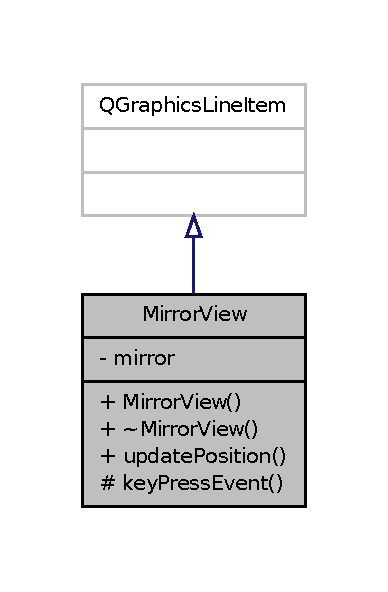
\includegraphics[width=186pt]{d2/d7b/classMirrorView__inherit__graph}
\end{center}
\end{figure}


Graphe de collaboration de Mirror\+View\+:\nopagebreak
\begin{figure}[H]
\begin{center}
\leavevmode
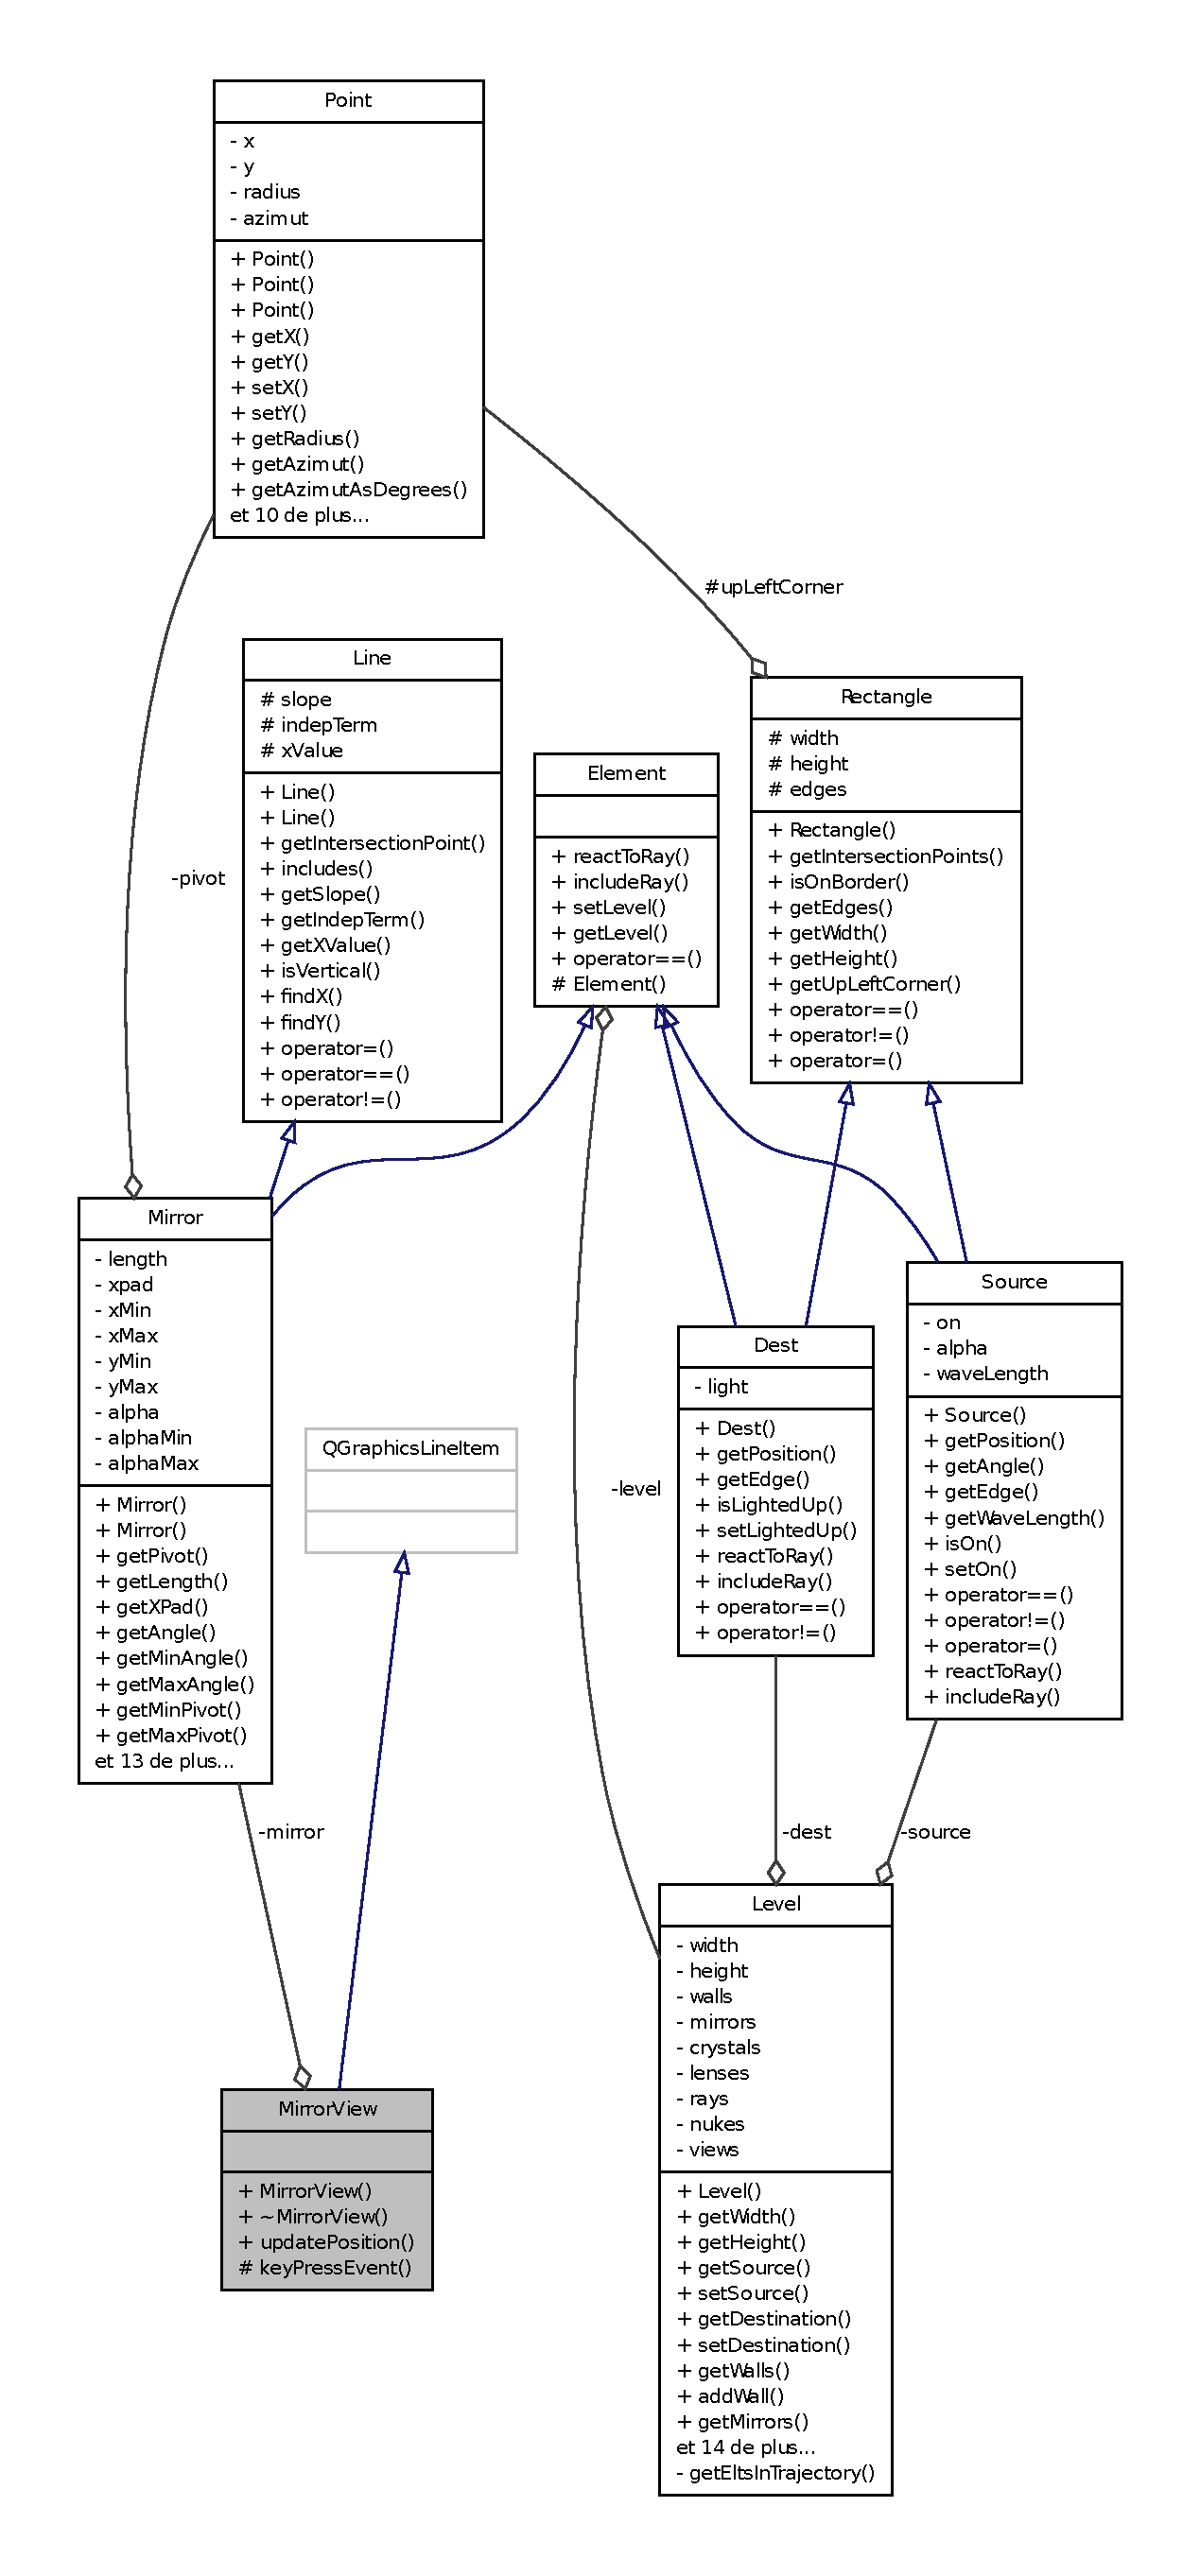
\includegraphics[height=550pt]{d1/de7/classMirrorView__coll__graph}
\end{center}
\end{figure}


\subsection{Documentation des constructeurs et destructeur}
\hypertarget{classMirrorView_adda194c3d1ae6827ba8490eb840c633a}{}\index{Mirror\+View@{Mirror\+View}!Mirror\+View@{Mirror\+View}}
\index{Mirror\+View@{Mirror\+View}!Mirror\+View@{Mirror\+View}}
\subsubsection[{Mirror\+View(\+Mirror $\ast$)}]{\setlength{\rightskip}{0pt plus 5cm}Mirror\+View\+::\+Mirror\+View (
\begin{DoxyParamCaption}
\item[{{\bf Mirror} $\ast$}]{}
\end{DoxyParamCaption}
)}\label{classMirrorView_adda194c3d1ae6827ba8490eb840c633a}


Construit une vue de miroir lié à un miroir. 


\begin{DoxyParams}{Paramètres}
{\em mirror} & Le miroir lié à cette vue. \\
\hline
\end{DoxyParams}
\hypertarget{classMirrorView_addbf31b1ac8687b9587b0b24a3d89fb0}{}\index{Mirror\+View@{Mirror\+View}!````~Mirror\+View@{$\sim$\+Mirror\+View}}
\index{````~Mirror\+View@{$\sim$\+Mirror\+View}!Mirror\+View@{Mirror\+View}}
\subsubsection[{$\sim$\+Mirror\+View()}]{\setlength{\rightskip}{0pt plus 5cm}Mirror\+View\+::$\sim$\+Mirror\+View (
\begin{DoxyParamCaption}
{}
\end{DoxyParamCaption}
)}\label{classMirrorView_addbf31b1ac8687b9587b0b24a3d89fb0}


Détruit le miroir. 



\subsection{Documentation des fonctions membres}
\hypertarget{classMirrorView_a1a9563cd71dd5a8e9a94d2245121e54c}{}\index{Mirror\+View@{Mirror\+View}!key\+Press\+Event@{key\+Press\+Event}}
\index{key\+Press\+Event@{key\+Press\+Event}!Mirror\+View@{Mirror\+View}}
\subsubsection[{key\+Press\+Event(\+Q\+Key\+Event $\ast$)}]{\setlength{\rightskip}{0pt plus 5cm}void Mirror\+View\+::key\+Press\+Event (
\begin{DoxyParamCaption}
\item[{Q\+Key\+Event $\ast$}]{}
\end{DoxyParamCaption}
)\hspace{0.3cm}{\ttfamily [protected]}}\label{classMirrorView_a1a9563cd71dd5a8e9a94d2245121e54c}


Permet de faire réagir le miroir à l\textquotesingle{}action de certaines touches du clavier et de la souris. 


\begin{DoxyParams}{Paramètres}
{\em event} & Une évènement \char`\"{}input user\char`\"{}. \\
\hline
\end{DoxyParams}
\hypertarget{classMirrorView_aa4a70f2a5c83b547631486660692ddf5}{}\index{Mirror\+View@{Mirror\+View}!update\+Position@{update\+Position}}
\index{update\+Position@{update\+Position}!Mirror\+View@{Mirror\+View}}
\subsubsection[{update\+Position()}]{\setlength{\rightskip}{0pt plus 5cm}void Mirror\+View\+::update\+Position (
\begin{DoxyParamCaption}
{}
\end{DoxyParamCaption}
)}\label{classMirrorView_aa4a70f2a5c83b547631486660692ddf5}


Permet de mettre à jour la position du mirroir. 



\subsection{Documentation des données membres}
\hypertarget{classMirrorView_aa470a75e02117480ff188e6a12583ffe}{}\index{Mirror\+View@{Mirror\+View}!mirror@{mirror}}
\index{mirror@{mirror}!Mirror\+View@{Mirror\+View}}
\subsubsection[{mirror}]{\setlength{\rightskip}{0pt plus 5cm}{\bf Mirror}$\ast$ Mirror\+View\+::mirror\hspace{0.3cm}{\ttfamily [private]}}\label{classMirrorView_aa470a75e02117480ff188e6a12583ffe}


Le miroir que cette vue représente. 



Définition à la ligne 18 du fichier mirrorview.\+hpp.



La documentation de cette classe a été générée à partir du fichier suivant \+:\begin{DoxyCompactItemize}
\item 
view/dynamic\+Elements/\hyperlink{mirrorview_8hpp}{mirrorview.\+hpp}\end{DoxyCompactItemize}

\hypertarget{classNuke}{}\section{Référence de la classe Nuke}
\label{classNuke}\index{Nuke@{Nuke}}


Cette classe modélise les bombes utilisées dans le jeu.  




{\ttfamily \#include $<$nuke.\+hpp$>$}

\subsection*{Fonctions membres publiques}
\begin{DoxyCompactItemize}
\item 
\hyperlink{classNuke_ab1b0d5faca4c5399b48e39774965fe62}{Nuke} (const \hyperlink{classPoint}{Point} \&, const double)
\begin{DoxyCompactList}\small\item\em Instancie une bombe en une position donnée avec un rayon déterminé. \end{DoxyCompactList}\item 
const \hyperlink{classPoint}{Point} \& \hyperlink{classNuke_a4cd753f8284d74613e91b46f94c6b678}{get\+Location} () const 
\begin{DoxyCompactList}\small\item\em Retourne la position de la bombe. \end{DoxyCompactList}\item 
double \hyperlink{classNuke_a4668365cff840c31886f35e9579bb1ac}{get\+Radius} () const 
\begin{DoxyCompactList}\small\item\em Retourne le rayon de la bombe. \end{DoxyCompactList}\item 
bool \hyperlink{classNuke_a85380caea565414da1ab78f4290fe1c8}{is\+Lighted\+Up} () const 
\begin{DoxyCompactList}\small\item\em Cette méthode permet de savoir si la bombe est illuminée. \end{DoxyCompactList}\item 
void \hyperlink{classNuke_a9abff8ef15814700c6a3a5f9f3962d25}{set\+Lighted\+Up} (const bool)
\begin{DoxyCompactList}\small\item\em Cette méthode permet d\textquotesingle{}établir un nouvel état d\textquotesingle{}illumination de la bombe. \end{DoxyCompactList}\item 
void \hyperlink{classNuke_a61433c8cba0b6e73c8c490f26bcbbe6b}{react\+To\+Ray} (\hyperlink{classRay}{Ray})
\begin{DoxyCompactList}\small\item\em Réaction à l\textquotesingle{}exposition d\textquotesingle{}un rayon. \end{DoxyCompactList}\item 
\hyperlink{classPoint}{Point} $\ast$ \hyperlink{classNuke_a36dfe7d835bc760a31525898f44ff675}{include\+Ray} (const \hyperlink{classRay}{Ray} \&) const 
\begin{DoxyCompactList}\small\item\em Renseigne si la bombe est dans la trajectoire du rayon. \end{DoxyCompactList}\item 
bool \hyperlink{classNuke_ae47302f18544028d0344da8cd31ccd6e}{operator==} (const \hyperlink{classNuke}{Nuke} \&) const 
\begin{DoxyCompactList}\small\item\em Permet de savoir si deux bombes sont les mêmes. \end{DoxyCompactList}\item 
bool \hyperlink{classNuke_a8970b5250d86dccd68e8d404aa22c53a}{operator!=} (const \hyperlink{classNuke}{Nuke} \&) const 
\begin{DoxyCompactList}\small\item\em Permet de savoir si deux bombes sont différentes. \end{DoxyCompactList}\end{DoxyCompactItemize}
\subsection*{Attributs privés}
\begin{DoxyCompactItemize}
\item 
bool \hyperlink{classNuke_a397479ffd9a1d1786a46c2a284b8234a}{light}
\begin{DoxyCompactList}\small\item\em L\textquotesingle{}état d\textquotesingle{}illumination d\textquotesingle{}une bombe. \end{DoxyCompactList}\end{DoxyCompactItemize}
\subsection*{Membres hérités additionnels}


\subsection{Description détaillée}
Cette classe modélise les bombes utilisées dans le jeu. 

Une bombe est un objet circulaire qui, si illuminé par un rayon, fait perdre la partie au joueur. 

Définition à la ligne 17 du fichier nuke.\+hpp.



Graphe d\textquotesingle{}héritage de Nuke\+:\nopagebreak
\begin{figure}[H]
\begin{center}
\leavevmode
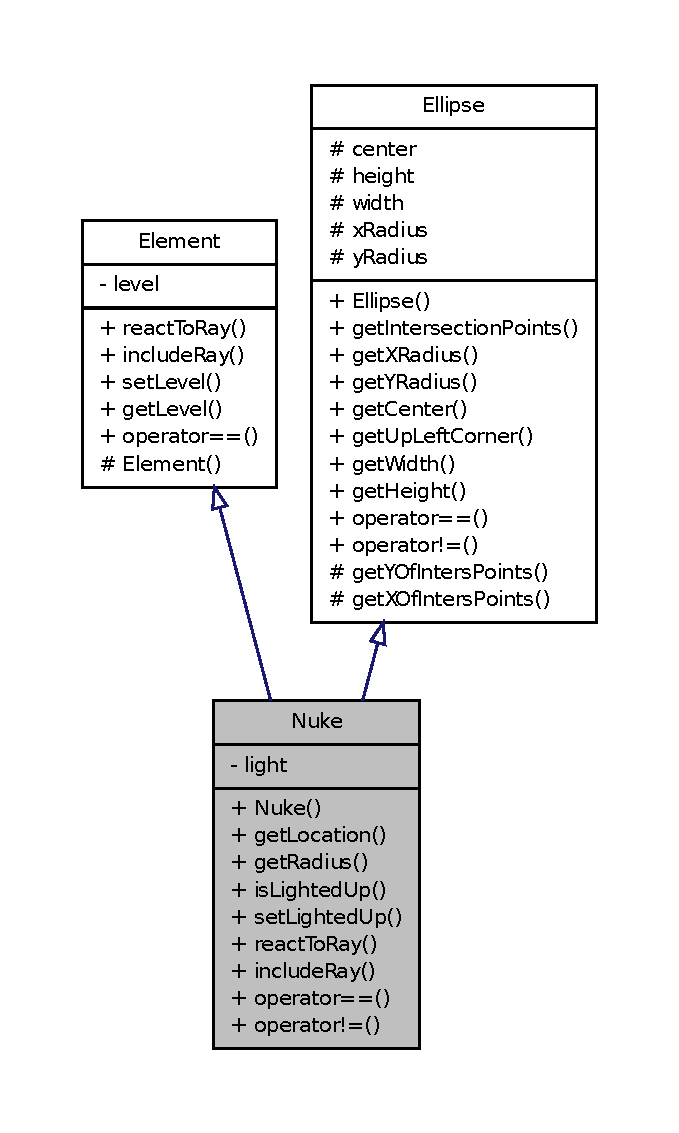
\includegraphics[width=326pt]{d7/d17/classNuke__inherit__graph}
\end{center}
\end{figure}


Graphe de collaboration de Nuke\+:\nopagebreak
\begin{figure}[H]
\begin{center}
\leavevmode
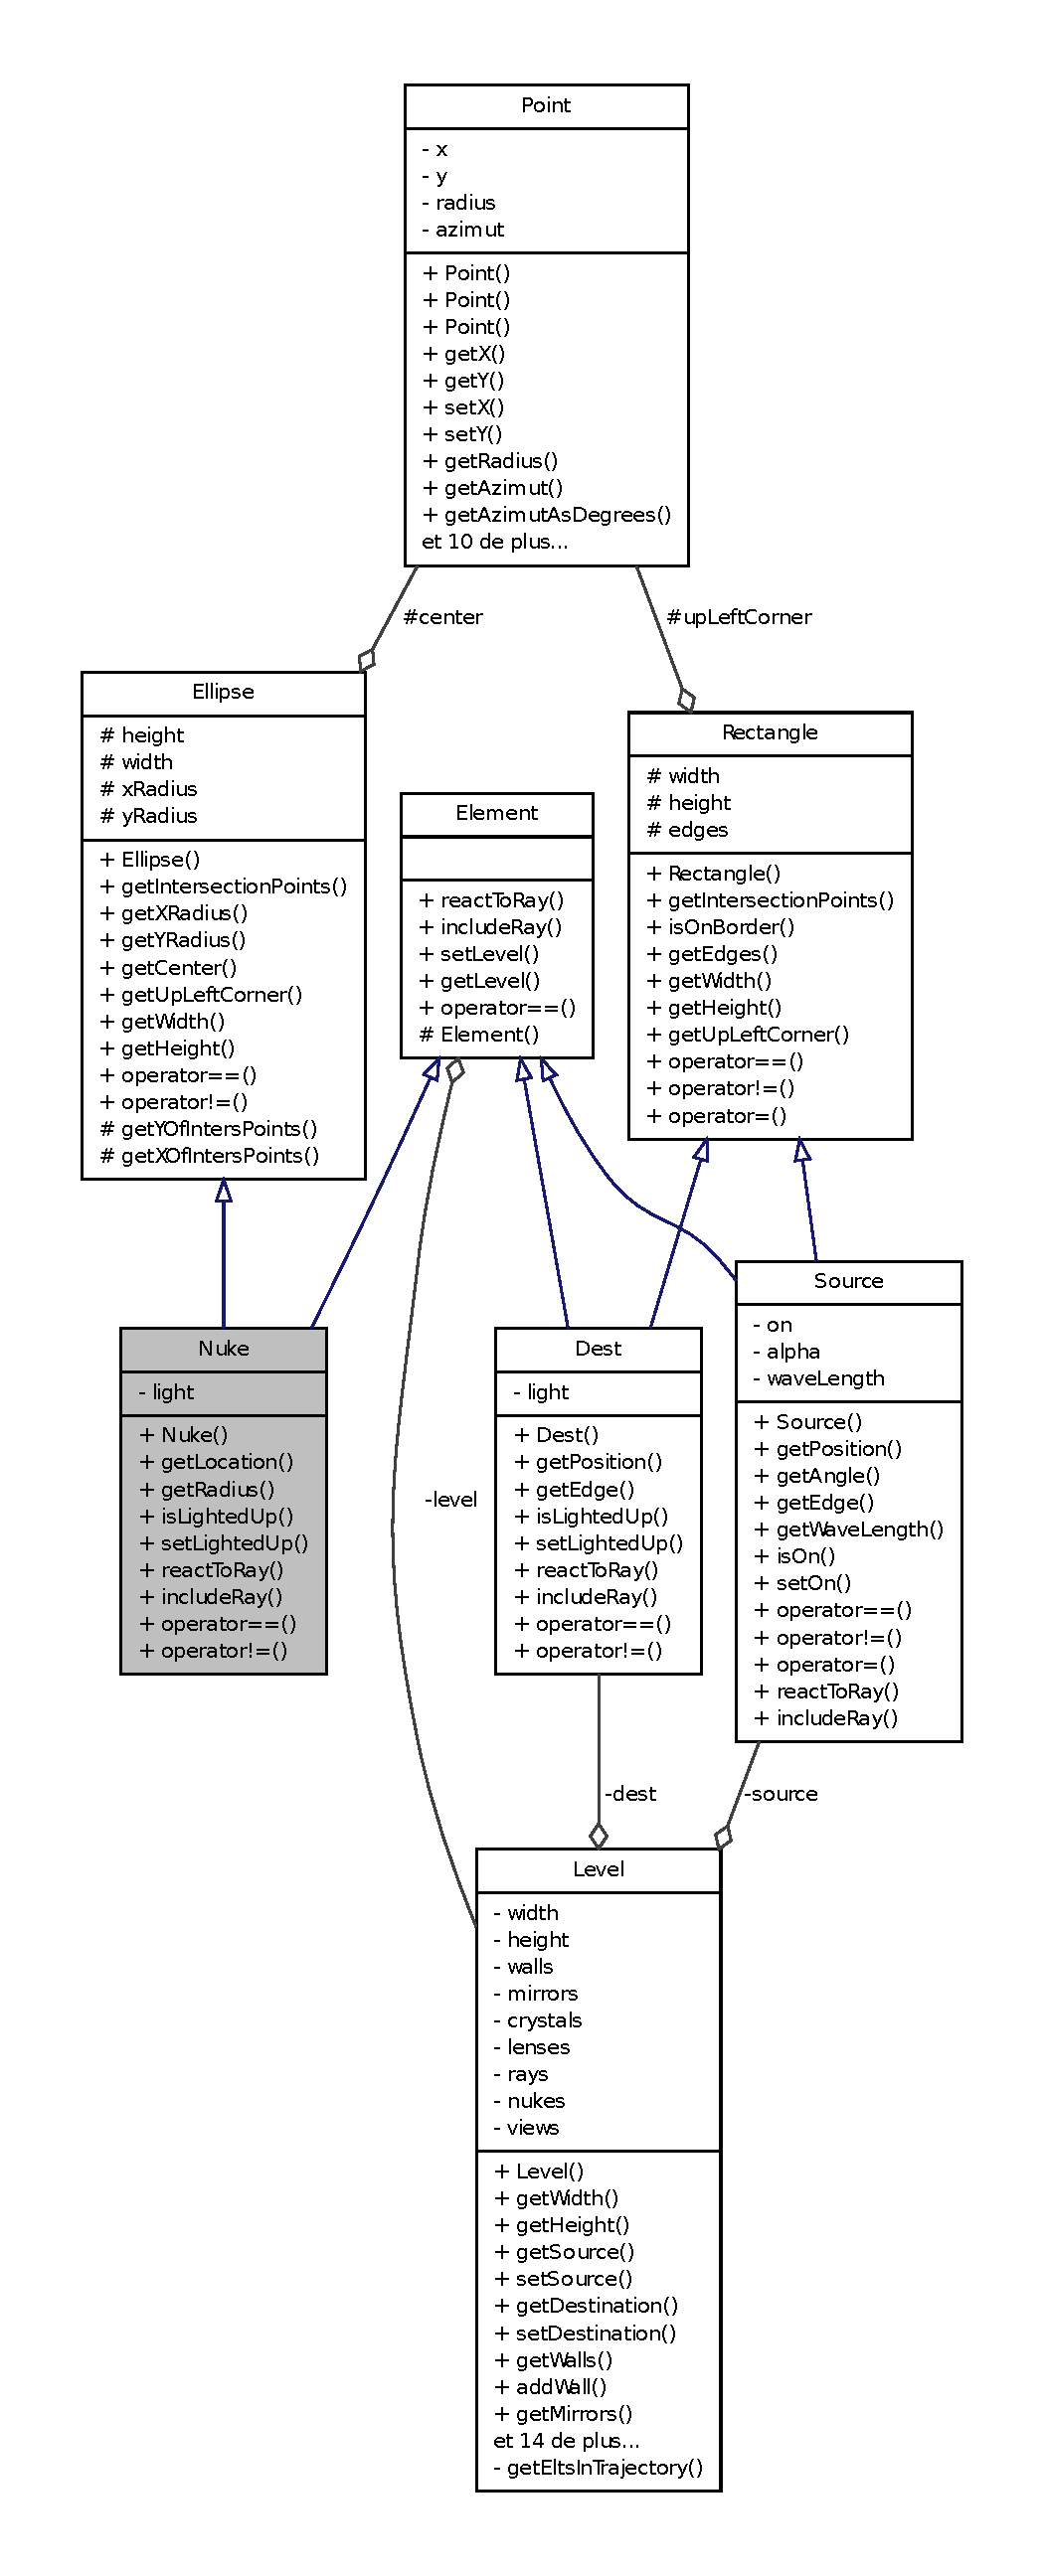
\includegraphics[height=550pt]{dc/d8c/classNuke__coll__graph}
\end{center}
\end{figure}


\subsection{Documentation des constructeurs et destructeur}
\hypertarget{classNuke_ab1b0d5faca4c5399b48e39774965fe62}{}\index{Nuke@{Nuke}!Nuke@{Nuke}}
\index{Nuke@{Nuke}!Nuke@{Nuke}}
\subsubsection[{Nuke(const Point \&, const double)}]{\setlength{\rightskip}{0pt plus 5cm}Nuke\+::\+Nuke (
\begin{DoxyParamCaption}
\item[{const {\bf Point} \&}]{, }
\item[{const double}]{}
\end{DoxyParamCaption}
)}\label{classNuke_ab1b0d5faca4c5399b48e39774965fe62}


Instancie une bombe en une position donnée avec un rayon déterminé. 


\begin{DoxyParams}{Paramètres}
{\em position} & La position du centre de la bombe. \\
\hline
{\em radius} & Le rayon de la bombe. \\
\hline
\end{DoxyParams}


\subsection{Documentation des fonctions membres}
\hypertarget{classNuke_a4cd753f8284d74613e91b46f94c6b678}{}\index{Nuke@{Nuke}!get\+Location@{get\+Location}}
\index{get\+Location@{get\+Location}!Nuke@{Nuke}}
\subsubsection[{get\+Location() const }]{\setlength{\rightskip}{0pt plus 5cm}const {\bf Point} \& Nuke\+::get\+Location (
\begin{DoxyParamCaption}
{}
\end{DoxyParamCaption}
) const\hspace{0.3cm}{\ttfamily [inline]}}\label{classNuke_a4cd753f8284d74613e91b46f94c6b678}


Retourne la position de la bombe. 

\begin{DoxyReturn}{Renvoie}
la position de la bombe. 
\end{DoxyReturn}


Définition à la ligne 107 du fichier nuke.\+hpp.



Références Ellipse\+::center.


\begin{DoxyCode}
108 \{
109     \textcolor{keywordflow}{return} this->\hyperlink{classEllipse_a88b27657adf698fded3a36fd97f90190}{center};
110 \}
\end{DoxyCode}
\hypertarget{classNuke_a4668365cff840c31886f35e9579bb1ac}{}\index{Nuke@{Nuke}!get\+Radius@{get\+Radius}}
\index{get\+Radius@{get\+Radius}!Nuke@{Nuke}}
\subsubsection[{get\+Radius() const }]{\setlength{\rightskip}{0pt plus 5cm}double Nuke\+::get\+Radius (
\begin{DoxyParamCaption}
{}
\end{DoxyParamCaption}
) const\hspace{0.3cm}{\ttfamily [inline]}}\label{classNuke_a4668365cff840c31886f35e9579bb1ac}


Retourne le rayon de la bombe. 

\begin{DoxyReturn}{Renvoie}
le rayon de la bombe. 
\end{DoxyReturn}


Définition à la ligne 112 du fichier nuke.\+hpp.



Références Ellipse\+::get\+Height().


\begin{DoxyCode}
113 \{
114     \textcolor{keywordflow}{return} (this->\hyperlink{classEllipse_aafb4efaa85efaf59e553c7423aa47b37}{getHeight}() / 2.);
115 \}
\end{DoxyCode}
\hypertarget{classNuke_a36dfe7d835bc760a31525898f44ff675}{}\index{Nuke@{Nuke}!include\+Ray@{include\+Ray}}
\index{include\+Ray@{include\+Ray}!Nuke@{Nuke}}
\subsubsection[{include\+Ray(const Ray \&) const }]{\setlength{\rightskip}{0pt plus 5cm}{\bf Point}$\ast$ Nuke\+::include\+Ray (
\begin{DoxyParamCaption}
\item[{const {\bf Ray} \&}]{}
\end{DoxyParamCaption}
) const\hspace{0.3cm}{\ttfamily [virtual]}}\label{classNuke_a36dfe7d835bc760a31525898f44ff675}


Renseigne si la bombe est dans la trajectoire du rayon. 


\begin{DoxyParams}{Paramètres}
{\em ray} & Le rayon.\\
\hline
\end{DoxyParams}
\begin{DoxyReturn}{Renvoie}
{\ttfamily true} Si la bombe se trouve dans la trajectoire du rayon entré en paramètre. 
\end{DoxyReturn}


Implémente \hyperlink{classElement_a1b88519623a6250155f7182706665448}{Element}.

\hypertarget{classNuke_a85380caea565414da1ab78f4290fe1c8}{}\index{Nuke@{Nuke}!is\+Lighted\+Up@{is\+Lighted\+Up}}
\index{is\+Lighted\+Up@{is\+Lighted\+Up}!Nuke@{Nuke}}
\subsubsection[{is\+Lighted\+Up() const }]{\setlength{\rightskip}{0pt plus 5cm}bool Nuke\+::is\+Lighted\+Up (
\begin{DoxyParamCaption}
{}
\end{DoxyParamCaption}
) const\hspace{0.3cm}{\ttfamily [inline]}}\label{classNuke_a85380caea565414da1ab78f4290fe1c8}


Cette méthode permet de savoir si la bombe est illuminée. 

\begin{DoxyReturn}{Renvoie}
{\ttfamily true} Si la bombe est illuminée, faux sinon. 
\end{DoxyReturn}


Définition à la ligne 102 du fichier nuke.\+hpp.



Références light.


\begin{DoxyCode}
103 \{
104     \textcolor{keywordflow}{return} this->\hyperlink{classNuke_a397479ffd9a1d1786a46c2a284b8234a}{light};
105 \}
\end{DoxyCode}
\hypertarget{classNuke_a8970b5250d86dccd68e8d404aa22c53a}{}\index{Nuke@{Nuke}!operator"!=@{operator"!=}}
\index{operator"!=@{operator"!=}!Nuke@{Nuke}}
\subsubsection[{operator"!=(const Nuke \&) const }]{\setlength{\rightskip}{0pt plus 5cm}bool Nuke\+::operator!= (
\begin{DoxyParamCaption}
\item[{const {\bf Nuke} \&}]{}
\end{DoxyParamCaption}
) const}\label{classNuke_a8970b5250d86dccd68e8d404aa22c53a}


Permet de savoir si deux bombes sont différentes. 

\begin{DoxyReturn}{Renvoie}
{\ttfamily true} Si les deux bombes sont différentes. 
\end{DoxyReturn}
\hypertarget{classNuke_ae47302f18544028d0344da8cd31ccd6e}{}\index{Nuke@{Nuke}!operator==@{operator==}}
\index{operator==@{operator==}!Nuke@{Nuke}}
\subsubsection[{operator==(const Nuke \&) const }]{\setlength{\rightskip}{0pt plus 5cm}bool Nuke\+::operator== (
\begin{DoxyParamCaption}
\item[{const {\bf Nuke} \&}]{}
\end{DoxyParamCaption}
) const}\label{classNuke_ae47302f18544028d0344da8cd31ccd6e}


Permet de savoir si deux bombes sont les mêmes. 

\begin{DoxyReturn}{Renvoie}
{\ttfamily true} Si les deux bombes sont les mêmes. 
\end{DoxyReturn}
\hypertarget{classNuke_a61433c8cba0b6e73c8c490f26bcbbe6b}{}\index{Nuke@{Nuke}!react\+To\+Ray@{react\+To\+Ray}}
\index{react\+To\+Ray@{react\+To\+Ray}!Nuke@{Nuke}}
\subsubsection[{react\+To\+Ray(\+Ray)}]{\setlength{\rightskip}{0pt plus 5cm}void Nuke\+::react\+To\+Ray (
\begin{DoxyParamCaption}
\item[{{\bf Ray}}]{}
\end{DoxyParamCaption}
)\hspace{0.3cm}{\ttfamily [virtual]}}\label{classNuke_a61433c8cba0b6e73c8c490f26bcbbe6b}


Réaction à l\textquotesingle{}exposition d\textquotesingle{}un rayon. 


\begin{DoxyParams}{Paramètres}
{\em ray} & Le rayon. \\
\hline
\end{DoxyParams}


Implémente \hyperlink{classElement_aa87116bb9422d64169b2ebf03831df9b}{Element}.

\hypertarget{classNuke_a9abff8ef15814700c6a3a5f9f3962d25}{}\index{Nuke@{Nuke}!set\+Lighted\+Up@{set\+Lighted\+Up}}
\index{set\+Lighted\+Up@{set\+Lighted\+Up}!Nuke@{Nuke}}
\subsubsection[{set\+Lighted\+Up(const bool)}]{\setlength{\rightskip}{0pt plus 5cm}void Nuke\+::set\+Lighted\+Up (
\begin{DoxyParamCaption}
\item[{const bool}]{}
\end{DoxyParamCaption}
)}\label{classNuke_a9abff8ef15814700c6a3a5f9f3962d25}


Cette méthode permet d\textquotesingle{}établir un nouvel état d\textquotesingle{}illumination de la bombe. 


\begin{DoxyParams}{Paramètres}
{\em light} & Le nouvel état d\textquotesingle{}illumination de la bombe. \\
\hline
\end{DoxyParams}


\subsection{Documentation des données membres}
\hypertarget{classNuke_a397479ffd9a1d1786a46c2a284b8234a}{}\index{Nuke@{Nuke}!light@{light}}
\index{light@{light}!Nuke@{Nuke}}
\subsubsection[{light}]{\setlength{\rightskip}{0pt plus 5cm}bool Nuke\+::light\hspace{0.3cm}{\ttfamily [private]}}\label{classNuke_a397479ffd9a1d1786a46c2a284b8234a}


L\textquotesingle{}état d\textquotesingle{}illumination d\textquotesingle{}une bombe. 



Définition à la ligne 22 du fichier nuke.\+hpp.



Référencé par is\+Lighted\+Up().



La documentation de cette classe a été générée à partir du fichier suivant \+:\begin{DoxyCompactItemize}
\item 
model/elements/\hyperlink{nuke_8hpp}{nuke.\+hpp}\end{DoxyCompactItemize}

\hypertarget{classPoint}{}\section{Référence de la classe Point}
\label{classPoint}\index{Point@{Point}}


Cette classe modélise un point de coordonnés dans le plan $ R^2 $ sous deux formes \+:  




{\ttfamily \#include $<$point.\+hpp$>$}

\subsection*{Fonctions membres publiques}
\begin{DoxyCompactItemize}
\item 
\hyperlink{classPoint_a257415ad611a16bb73628efcdb87d0fd}{Point} ()=default
\begin{DoxyCompactList}\small\item\em Instancie le point $c(0, 0) p(0, 0)$. \end{DoxyCompactList}\item 
\hyperlink{classPoint_a370ac864b989b581ce00c674d722d77d}{Point} (const double, const double)
\begin{DoxyCompactList}\small\item\em Instancie le point de coordonnées spécifiées. \end{DoxyCompactList}\item 
\hyperlink{classPoint_a5b7ec0fb127734c1cd5c6f350a3990fc}{Point} (const \hyperlink{classPoint}{Point} \&)
\begin{DoxyCompactList}\small\item\em Instancie un point par copie d\textquotesingle{}un autre point \+: constructeur de recopie. \end{DoxyCompactList}\item 
double \hyperlink{classPoint_af52a20a376f8f31e87658837565d3812}{get\+X} () const 
\begin{DoxyCompactList}\small\item\em Retourne l\textquotesingle{}abscisse du point. \end{DoxyCompactList}\item 
double \hyperlink{classPoint_aac5008459bf0e0053ce744a69187bae7}{get\+Y} () const 
\begin{DoxyCompactList}\small\item\em Retourne l\textquotesingle{}ordonnée du point. \end{DoxyCompactList}\item 
void \hyperlink{classPoint_a59ad664629f66d7faa5a97c222b11e53}{set\+X} (const double)
\begin{DoxyCompactList}\small\item\em Déplace le point en l\textquotesingle{}abscisse donnée. \end{DoxyCompactList}\item 
void \hyperlink{classPoint_a62d94bacca48640df1beb272527e0c75}{set\+Y} (const double)
\begin{DoxyCompactList}\small\item\em Déplace le point en l\textquotesingle{}ordonnée donnée. \end{DoxyCompactList}\item 
double \hyperlink{classPoint_a9109d60b782e753cc08bbdf4c5e6e4c7}{get\+Radius} () const 
\begin{DoxyCompactList}\small\item\em Permet d\textquotesingle{}obtenir la distance séparant le point du centre de rotation. \end{DoxyCompactList}\item 
double \hyperlink{classPoint_a29aedc573ec7cb54b2988cb5d5663e57}{get\+Azimut} () const 
\begin{DoxyCompactList}\small\item\em Permet d\textquotesingle{}obtenir l\textquotesingle{}angle de la coordonnée polaire courante. \end{DoxyCompactList}\item 
double \hyperlink{classPoint_a5208a853813f8a17c038f90f7434c458}{get\+Azimut\+As\+Degrees} () const 
\begin{DoxyCompactList}\small\item\em Permet d\textquotesingle{}obtenir l\textquotesingle{}angle de la coordonnée polaire courante exprimée en degrés. \end{DoxyCompactList}\item 
\hyperlink{classPoint}{Point} \& \hyperlink{classPoint_a681473d41e1569769f9fcfe1f49a1855}{rotate\+Around} (const \hyperlink{classPoint}{Point} \&, const double)
\begin{DoxyCompactList}\small\item\em Cette méthode change la position du point courant dans le plan par rotation autour du point cartésien passé en paramètre. \end{DoxyCompactList}\item 
void \hyperlink{classPoint_a7fb8d07f5e6b6e49c0f2322356c0fe8d}{rotate} (const double)
\begin{DoxyCompactList}\small\item\em Effectue une rotation autour de l\textquotesingle{}origine du plan cartésien. \end{DoxyCompactList}\item 
void \hyperlink{classPoint_aab46bd6d93ccf0e90d3c4676d5cd40d1}{set\+Origin} (const \hyperlink{classPoint}{Point} \&=\hyperlink{classPoint}{Point}\{0., 0.\})
\begin{DoxyCompactList}\small\item\em Considère la position d\textquotesingle{}un point par rapport à un point quelconque. \end{DoxyCompactList}\item 
void \hyperlink{classPoint_a8e18fe044163b18acaefcda0a36b8fa3}{extend} (const double)
\begin{DoxyCompactList}\small\item\em Modifie le point pour lui donner un position de même angle en lui ajoutant un radius. \end{DoxyCompactList}\item 
void \hyperlink{classPoint_a292f3e944f1e11d1147480868ac01e99}{set\+Cartesian\+Location} (const double, const double)
\begin{DoxyCompactList}\small\item\em Déplace le point en la coordonnée cartésienne donnée. \end{DoxyCompactList}\item 
void \hyperlink{classPoint_a17a63e4dcb905423c0630ee127fffcae}{set\+Polar\+Location} (const double, const double)
\begin{DoxyCompactList}\small\item\em Déplace le point en la coordonnée polaire donnée. \end{DoxyCompactList}\item 
double \hyperlink{classPoint_ad3f543f2b8cd6a61399a3992e48769e0}{distance\+From} (const \hyperlink{classPoint}{Point} \&) const 
\begin{DoxyCompactList}\small\item\em Permet de connaitre la distance séparant le point courant d\textquotesingle{}un autre. \end{DoxyCompactList}\item 
\hyperlink{classPoint}{Point} \& \hyperlink{classPoint_aecfc6968998d806384e24cd93072b024}{operator=} (const \hyperlink{classPoint}{Point} \&)
\begin{DoxyCompactList}\small\item\em Permet de copier le contenu d\textquotesingle{}un point dans un autre point. \end{DoxyCompactList}\item 
bool \hyperlink{classPoint_aacbb5ae0d9898c4648e9d49441c029ce}{operator==} (const \hyperlink{classPoint}{Point} \&) const 
\begin{DoxyCompactList}\small\item\em Permet de savoir si deux points sont aux même endroit. \end{DoxyCompactList}\item 
bool \hyperlink{classPoint_a627f69d792993405c27b64387c77432b}{operator!=} (const \hyperlink{classPoint}{Point} \&) const 
\begin{DoxyCompactList}\small\item\em Permet de savoir si deux points ne sont pas au même endroit. \end{DoxyCompactList}\end{DoxyCompactItemize}
\subsection*{Attributs privés}
\begin{DoxyCompactItemize}
\item 
double \hyperlink{classPoint_ab99c56589bc8ad5fa5071387110a5bc7}{x} \{0.\}
\begin{DoxyCompactList}\small\item\em x La distance, sur l\textquotesingle{}axe des abscisses, du point par rapport à l\textquotesingle{}origine. \end{DoxyCompactList}\item 
double \hyperlink{classPoint_afa38be143ae800e6ad69ce8ed4df62d8}{y} \{0.\}
\begin{DoxyCompactList}\small\item\em y La distance, sur l\textquotesingle{}axe des ordonnées, du point par rapport à l\textquotesingle{}origine. \end{DoxyCompactList}\item 
double \hyperlink{classPoint_af4f987f16754db370e5d1b3d1bf1fd52}{radius} \{0.\}
\begin{DoxyCompactList}\small\item\em radius la distance du point par rapport à l\textquotesingle{}origine du plan cartésien. \end{DoxyCompactList}\item 
double \hyperlink{classPoint_a873c221d6bc33e2108574d6f1c911f78}{azimut} \{0.\}
\begin{DoxyCompactList}\small\item\em azimut le segment de cercle exprimé en radian depuis l\textquotesingle{}axe horizontal et dans un sens anti-\/horloger. \end{DoxyCompactList}\end{DoxyCompactItemize}


\subsection{Description détaillée}
Cette classe modélise un point de coordonnés dans le plan $ R^2 $ sous deux formes \+: 


\begin{DoxyItemize}
\item coordonnées cartésiennes sous la forme $ c(x, y) $, 
\item coordonnées polaires sous la forme $ p(r, \alpha) $. 
\end{DoxyItemize}Elle sert à définir la position d\textquotesingle{}un objet dans l\textquotesingle{}espace à deux dimensions. 

Définition à la ligne 15 du fichier point.\+hpp.



Graphe de collaboration de Point\+:\nopagebreak
\begin{figure}[H]
\begin{center}
\leavevmode
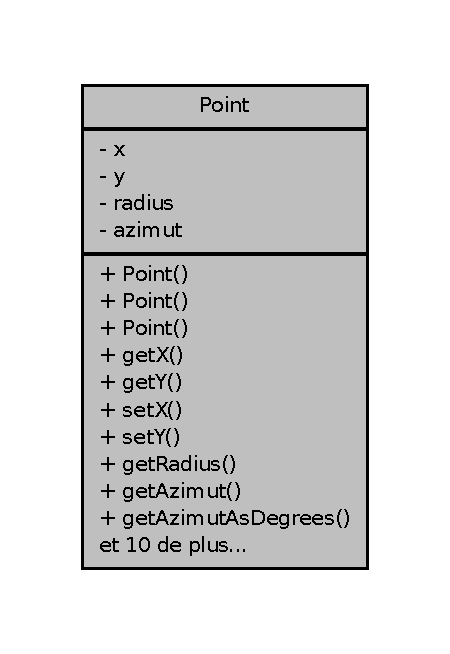
\includegraphics[width=216pt]{d5/d3b/classPoint__coll__graph}
\end{center}
\end{figure}


\subsection{Documentation des constructeurs et destructeur}
\hypertarget{classPoint_a257415ad611a16bb73628efcdb87d0fd}{}\index{Point@{Point}!Point@{Point}}
\index{Point@{Point}!Point@{Point}}
\subsubsection[{Point()=default}]{\setlength{\rightskip}{0pt plus 5cm}Point\+::\+Point (
\begin{DoxyParamCaption}
{}
\end{DoxyParamCaption}
)\hspace{0.3cm}{\ttfamily [default]}}\label{classPoint_a257415ad611a16bb73628efcdb87d0fd}


Instancie le point $c(0, 0) p(0, 0)$. 

\hypertarget{classPoint_a370ac864b989b581ce00c674d722d77d}{}\index{Point@{Point}!Point@{Point}}
\index{Point@{Point}!Point@{Point}}
\subsubsection[{Point(const double, const double)}]{\setlength{\rightskip}{0pt plus 5cm}Point\+::\+Point (
\begin{DoxyParamCaption}
\item[{const double}]{, }
\item[{const double}]{}
\end{DoxyParamCaption}
)}\label{classPoint_a370ac864b989b581ce00c674d722d77d}


Instancie le point de coordonnées spécifiées. 


\begin{DoxyParams}{Paramètres}
{\em x} & l\textquotesingle{}abscisse du point \\
\hline
{\em y} & l\textquotesingle{}ordonnée du point \\
\hline
\end{DoxyParams}
\hypertarget{classPoint_a5b7ec0fb127734c1cd5c6f350a3990fc}{}\index{Point@{Point}!Point@{Point}}
\index{Point@{Point}!Point@{Point}}
\subsubsection[{Point(const Point \&)}]{\setlength{\rightskip}{0pt plus 5cm}Point\+::\+Point (
\begin{DoxyParamCaption}
\item[{const {\bf Point} \&}]{}
\end{DoxyParamCaption}
)}\label{classPoint_a5b7ec0fb127734c1cd5c6f350a3990fc}


Instancie un point par copie d\textquotesingle{}un autre point \+: constructeur de recopie. 



\subsection{Documentation des fonctions membres}
\hypertarget{classPoint_ad3f543f2b8cd6a61399a3992e48769e0}{}\index{Point@{Point}!distance\+From@{distance\+From}}
\index{distance\+From@{distance\+From}!Point@{Point}}
\subsubsection[{distance\+From(const Point \&) const }]{\setlength{\rightskip}{0pt plus 5cm}double Point\+::distance\+From (
\begin{DoxyParamCaption}
\item[{const {\bf Point} \&}]{}
\end{DoxyParamCaption}
) const}\label{classPoint_ad3f543f2b8cd6a61399a3992e48769e0}


Permet de connaitre la distance séparant le point courant d\textquotesingle{}un autre. 

La distance est calculée à l\textquotesingle{}aide du théorème de Pythagore au triangle rectangle \+: soient les deux points du plan cartésien reliés formant un segment de droite, en traçant les parallèles aux axes passant par ces points on peut délimiter un triangle rectangle par l\textquotesingle{}intersection des deux droites. De là, il est simple d\textquotesingle{}appliquer le théorème de Pythagore aux triangles rectangles \+: l\textquotesingle{}hypoténuse au carré = la somme du carré des deux autres cotés $ distance(p1, p2)^2 = (p1.x - p2.x)^2 + (p1.y - p2.y)^2 $ Dans la bibliothèque standard C++, la fonction std\+::hypot de $<$cmath$>$ nous permet de faire cette opération en lui passant simplement les cotés autre que l\textquotesingle{}hypoténuse. 
\begin{DoxyParams}{Paramètres}
{\em point} & Un autre point. \\
\hline
\end{DoxyParams}
\begin{DoxyReturn}{Renvoie}
La distance séparant deux point. 
\end{DoxyReturn}
\hypertarget{classPoint_a8e18fe044163b18acaefcda0a36b8fa3}{}\index{Point@{Point}!extend@{extend}}
\index{extend@{extend}!Point@{Point}}
\subsubsection[{extend(const double)}]{\setlength{\rightskip}{0pt plus 5cm}void Point\+::extend (
\begin{DoxyParamCaption}
\item[{const double}]{}
\end{DoxyParamCaption}
)}\label{classPoint_a8e18fe044163b18acaefcda0a36b8fa3}


Modifie le point pour lui donner un position de même angle en lui ajoutant un radius. 


\begin{DoxyParams}{Paramètres}
{\em radius} & Un nouveau radius. \\
\hline
\end{DoxyParams}
\hypertarget{classPoint_a29aedc573ec7cb54b2988cb5d5663e57}{}\index{Point@{Point}!get\+Azimut@{get\+Azimut}}
\index{get\+Azimut@{get\+Azimut}!Point@{Point}}
\subsubsection[{get\+Azimut() const }]{\setlength{\rightskip}{0pt plus 5cm}double Point\+::get\+Azimut (
\begin{DoxyParamCaption}
{}
\end{DoxyParamCaption}
) const\hspace{0.3cm}{\ttfamily [inline]}}\label{classPoint_a29aedc573ec7cb54b2988cb5d5663e57}


Permet d\textquotesingle{}obtenir l\textquotesingle{}angle de la coordonnée polaire courante. 

\begin{DoxyReturn}{Renvoie}
L\textquotesingle{}amplitude du point polaire courant en radian. 
\end{DoxyReturn}


Définition à la ligne 220 du fichier point.\+hpp.



Références azimut.


\begin{DoxyCode}
221 \{
222     \textcolor{keywordflow}{return} this->\hyperlink{classPoint_a873c221d6bc33e2108574d6f1c911f78}{azimut};
223 \}
\end{DoxyCode}
\hypertarget{classPoint_a5208a853813f8a17c038f90f7434c458}{}\index{Point@{Point}!get\+Azimut\+As\+Degrees@{get\+Azimut\+As\+Degrees}}
\index{get\+Azimut\+As\+Degrees@{get\+Azimut\+As\+Degrees}!Point@{Point}}
\subsubsection[{get\+Azimut\+As\+Degrees() const }]{\setlength{\rightskip}{0pt plus 5cm}double Point\+::get\+Azimut\+As\+Degrees (
\begin{DoxyParamCaption}
{}
\end{DoxyParamCaption}
) const}\label{classPoint_a5208a853813f8a17c038f90f7434c458}


Permet d\textquotesingle{}obtenir l\textquotesingle{}angle de la coordonnée polaire courante exprimée en degrés. 

\begin{DoxyReturn}{Renvoie}
L\textquotesingle{}amplitude du point polaire courant en degré. 
\end{DoxyReturn}
\hypertarget{classPoint_a9109d60b782e753cc08bbdf4c5e6e4c7}{}\index{Point@{Point}!get\+Radius@{get\+Radius}}
\index{get\+Radius@{get\+Radius}!Point@{Point}}
\subsubsection[{get\+Radius() const }]{\setlength{\rightskip}{0pt plus 5cm}double Point\+::get\+Radius (
\begin{DoxyParamCaption}
{}
\end{DoxyParamCaption}
) const\hspace{0.3cm}{\ttfamily [inline]}}\label{classPoint_a9109d60b782e753cc08bbdf4c5e6e4c7}


Permet d\textquotesingle{}obtenir la distance séparant le point du centre de rotation. 

\begin{DoxyReturn}{Renvoie}
Le rayon séparant le point polaire de son centre. 
\end{DoxyReturn}


Définition à la ligne 215 du fichier point.\+hpp.



Références radius.


\begin{DoxyCode}
216 \{
217     \textcolor{keywordflow}{return} this->\hyperlink{classPoint_af4f987f16754db370e5d1b3d1bf1fd52}{radius};
218 \}
\end{DoxyCode}
\hypertarget{classPoint_af52a20a376f8f31e87658837565d3812}{}\index{Point@{Point}!get\+X@{get\+X}}
\index{get\+X@{get\+X}!Point@{Point}}
\subsubsection[{get\+X() const }]{\setlength{\rightskip}{0pt plus 5cm}double Point\+::get\+X (
\begin{DoxyParamCaption}
{}
\end{DoxyParamCaption}
) const\hspace{0.3cm}{\ttfamily [inline]}}\label{classPoint_af52a20a376f8f31e87658837565d3812}


Retourne l\textquotesingle{}abscisse du point. 

\begin{DoxyReturn}{Renvoie}
l\textquotesingle{}abscisse du point. 
\end{DoxyReturn}


Définition à la ligne 205 du fichier point.\+hpp.



Références x.


\begin{DoxyCode}
206 \{
207     \textcolor{keywordflow}{return} this->\hyperlink{classPoint_ab99c56589bc8ad5fa5071387110a5bc7}{x};
208 \}
\end{DoxyCode}
\hypertarget{classPoint_aac5008459bf0e0053ce744a69187bae7}{}\index{Point@{Point}!get\+Y@{get\+Y}}
\index{get\+Y@{get\+Y}!Point@{Point}}
\subsubsection[{get\+Y() const }]{\setlength{\rightskip}{0pt plus 5cm}double Point\+::get\+Y (
\begin{DoxyParamCaption}
{}
\end{DoxyParamCaption}
) const\hspace{0.3cm}{\ttfamily [inline]}}\label{classPoint_aac5008459bf0e0053ce744a69187bae7}


Retourne l\textquotesingle{}ordonnée du point. 

\begin{DoxyReturn}{Renvoie}
l\textquotesingle{}ordonnée du point. 
\end{DoxyReturn}


Définition à la ligne 210 du fichier point.\+hpp.



Références y.


\begin{DoxyCode}
211 \{
212     \textcolor{keywordflow}{return} this->\hyperlink{classPoint_afa38be143ae800e6ad69ce8ed4df62d8}{y};
213 \}
\end{DoxyCode}
\hypertarget{classPoint_a627f69d792993405c27b64387c77432b}{}\index{Point@{Point}!operator"!=@{operator"!=}}
\index{operator"!=@{operator"!=}!Point@{Point}}
\subsubsection[{operator"!=(const Point \&) const }]{\setlength{\rightskip}{0pt plus 5cm}bool Point\+::operator!= (
\begin{DoxyParamCaption}
\item[{const {\bf Point} \&}]{}
\end{DoxyParamCaption}
) const}\label{classPoint_a627f69d792993405c27b64387c77432b}


Permet de savoir si deux points ne sont pas au même endroit. 

\begin{DoxyReturn}{Renvoie}
{\ttfamily true} Si les deux points ne sont pas les mêmes. 
\end{DoxyReturn}
\hypertarget{classPoint_aecfc6968998d806384e24cd93072b024}{}\index{Point@{Point}!operator=@{operator=}}
\index{operator=@{operator=}!Point@{Point}}
\subsubsection[{operator=(const Point \&)}]{\setlength{\rightskip}{0pt plus 5cm}{\bf Point}\& Point\+::operator= (
\begin{DoxyParamCaption}
\item[{const {\bf Point} \&}]{}
\end{DoxyParamCaption}
)}\label{classPoint_aecfc6968998d806384e24cd93072b024}


Permet de copier le contenu d\textquotesingle{}un point dans un autre point. 

\begin{DoxyReturn}{Renvoie}
Le point courant modifié. 
\end{DoxyReturn}
\hypertarget{classPoint_aacbb5ae0d9898c4648e9d49441c029ce}{}\index{Point@{Point}!operator==@{operator==}}
\index{operator==@{operator==}!Point@{Point}}
\subsubsection[{operator==(const Point \&) const }]{\setlength{\rightskip}{0pt plus 5cm}bool Point\+::operator== (
\begin{DoxyParamCaption}
\item[{const {\bf Point} \&}]{}
\end{DoxyParamCaption}
) const}\label{classPoint_aacbb5ae0d9898c4648e9d49441c029ce}


Permet de savoir si deux points sont aux même endroit. 

\begin{DoxyReturn}{Renvoie}
{\ttfamily true} Si les deux points ont les même coordonnées. 
\end{DoxyReturn}
\hypertarget{classPoint_a7fb8d07f5e6b6e49c0f2322356c0fe8d}{}\index{Point@{Point}!rotate@{rotate}}
\index{rotate@{rotate}!Point@{Point}}
\subsubsection[{rotate(const double)}]{\setlength{\rightskip}{0pt plus 5cm}void Point\+::rotate (
\begin{DoxyParamCaption}
\item[{const double}]{}
\end{DoxyParamCaption}
)}\label{classPoint_a7fb8d07f5e6b6e49c0f2322356c0fe8d}


Effectue une rotation autour de l\textquotesingle{}origine du plan cartésien. 


\begin{DoxyParams}{Paramètres}
{\em alpha} & L\textquotesingle{}amplitude de la rotation à effectuer (en radian). \\
\hline
\end{DoxyParams}
\hypertarget{classPoint_a681473d41e1569769f9fcfe1f49a1855}{}\index{Point@{Point}!rotate\+Around@{rotate\+Around}}
\index{rotate\+Around@{rotate\+Around}!Point@{Point}}
\subsubsection[{rotate\+Around(const Point \&, const double)}]{\setlength{\rightskip}{0pt plus 5cm}{\bf Point}\& Point\+::rotate\+Around (
\begin{DoxyParamCaption}
\item[{const {\bf Point} \&}]{, }
\item[{const double}]{}
\end{DoxyParamCaption}
)}\label{classPoint_a681473d41e1569769f9fcfe1f49a1855}


Cette méthode change la position du point courant dans le plan par rotation autour du point cartésien passé en paramètre. 


\begin{DoxyParams}{Paramètres}
{\em pivot} & Le centre autour duquel le point courant doit tourner. \\
\hline
{\em alpha} & L\textquotesingle{}amplitude de la rotation à effectuer (en radian).\\
\hline
\end{DoxyParams}
\begin{DoxyReturn}{Renvoie}
Le point courant après rotation. 
\end{DoxyReturn}
\hypertarget{classPoint_a292f3e944f1e11d1147480868ac01e99}{}\index{Point@{Point}!set\+Cartesian\+Location@{set\+Cartesian\+Location}}
\index{set\+Cartesian\+Location@{set\+Cartesian\+Location}!Point@{Point}}
\subsubsection[{set\+Cartesian\+Location(const double, const double)}]{\setlength{\rightskip}{0pt plus 5cm}void Point\+::set\+Cartesian\+Location (
\begin{DoxyParamCaption}
\item[{const double}]{, }
\item[{const double}]{}
\end{DoxyParamCaption}
)}\label{classPoint_a292f3e944f1e11d1147480868ac01e99}


Déplace le point en la coordonnée cartésienne donnée. 


\begin{DoxyParams}{Paramètres}
{\em x} & l\textquotesingle{}abscisse où déplacer le point. \\
\hline
{\em y} & l\textquotesingle{}ordonnée où déplacer le point. \\
\hline
\end{DoxyParams}
\hypertarget{classPoint_aab46bd6d93ccf0e90d3c4676d5cd40d1}{}\index{Point@{Point}!set\+Origin@{set\+Origin}}
\index{set\+Origin@{set\+Origin}!Point@{Point}}
\subsubsection[{set\+Origin(const Point \&=\+Point\lcurly{}0., 0.\rcurly{})}]{\setlength{\rightskip}{0pt plus 5cm}void Point\+::set\+Origin (
\begin{DoxyParamCaption}
\item[{const {\bf Point} \&}]{ = {\ttfamily {\bf Point}\{0.,~0.\}}}
\end{DoxyParamCaption}
)}\label{classPoint_aab46bd6d93ccf0e90d3c4676d5cd40d1}


Considère la position d\textquotesingle{}un point par rapport à un point quelconque. 


\begin{DoxyParams}{Paramètres}
{\em origin} & La nouvelle origine du plan. Si ce paramètre est omis, l\textquotesingle{}origine du plan est rétabli. \\
\hline
\end{DoxyParams}
\hypertarget{classPoint_a17a63e4dcb905423c0630ee127fffcae}{}\index{Point@{Point}!set\+Polar\+Location@{set\+Polar\+Location}}
\index{set\+Polar\+Location@{set\+Polar\+Location}!Point@{Point}}
\subsubsection[{set\+Polar\+Location(const double, const double)}]{\setlength{\rightskip}{0pt plus 5cm}void Point\+::set\+Polar\+Location (
\begin{DoxyParamCaption}
\item[{const double}]{, }
\item[{const double}]{}
\end{DoxyParamCaption}
)}\label{classPoint_a17a63e4dcb905423c0630ee127fffcae}


Déplace le point en la coordonnée polaire donnée. 


\begin{DoxyParams}{Paramètres}
{\em radius} & La distance séparant le point de l\textquotesingle{}origine. \\
\hline
{\em azimut} & L\textquotesingle{}angle, en radian, selon le cercle trigonométrique. \\
\hline
\end{DoxyParams}
\hypertarget{classPoint_a59ad664629f66d7faa5a97c222b11e53}{}\index{Point@{Point}!set\+X@{set\+X}}
\index{set\+X@{set\+X}!Point@{Point}}
\subsubsection[{set\+X(const double)}]{\setlength{\rightskip}{0pt plus 5cm}void Point\+::set\+X (
\begin{DoxyParamCaption}
\item[{const double}]{}
\end{DoxyParamCaption}
)}\label{classPoint_a59ad664629f66d7faa5a97c222b11e53}


Déplace le point en l\textquotesingle{}abscisse donnée. 


\begin{DoxyParams}{Paramètres}
{\em x} & l\textquotesingle{}abscisse où déplacer le point. \\
\hline
\end{DoxyParams}
\hypertarget{classPoint_a62d94bacca48640df1beb272527e0c75}{}\index{Point@{Point}!set\+Y@{set\+Y}}
\index{set\+Y@{set\+Y}!Point@{Point}}
\subsubsection[{set\+Y(const double)}]{\setlength{\rightskip}{0pt plus 5cm}void Point\+::set\+Y (
\begin{DoxyParamCaption}
\item[{const double}]{}
\end{DoxyParamCaption}
)}\label{classPoint_a62d94bacca48640df1beb272527e0c75}


Déplace le point en l\textquotesingle{}ordonnée donnée. 


\begin{DoxyParams}{Paramètres}
{\em y} & l\textquotesingle{}ordonnée où déplacer le point. \\
\hline
\end{DoxyParams}


\subsection{Documentation des données membres}
\hypertarget{classPoint_a873c221d6bc33e2108574d6f1c911f78}{}\index{Point@{Point}!azimut@{azimut}}
\index{azimut@{azimut}!Point@{Point}}
\subsubsection[{azimut}]{\setlength{\rightskip}{0pt plus 5cm}double Point\+::azimut \{0.\}\hspace{0.3cm}{\ttfamily [private]}}\label{classPoint_a873c221d6bc33e2108574d6f1c911f78}


azimut le segment de cercle exprimé en radian depuis l\textquotesingle{}axe horizontal et dans un sens anti-\/horloger. 



Définition à la ligne 41 du fichier point.\+hpp.



Référencé par get\+Azimut().

\hypertarget{classPoint_af4f987f16754db370e5d1b3d1bf1fd52}{}\index{Point@{Point}!radius@{radius}}
\index{radius@{radius}!Point@{Point}}
\subsubsection[{radius}]{\setlength{\rightskip}{0pt plus 5cm}double Point\+::radius \{0.\}\hspace{0.3cm}{\ttfamily [private]}}\label{classPoint_af4f987f16754db370e5d1b3d1bf1fd52}


radius la distance du point par rapport à l\textquotesingle{}origine du plan cartésien. 



Définition à la ligne 35 du fichier point.\+hpp.



Référencé par get\+Radius().

\hypertarget{classPoint_ab99c56589bc8ad5fa5071387110a5bc7}{}\index{Point@{Point}!x@{x}}
\index{x@{x}!Point@{Point}}
\subsubsection[{x}]{\setlength{\rightskip}{0pt plus 5cm}double Point\+::x \{0.\}\hspace{0.3cm}{\ttfamily [private]}}\label{classPoint_ab99c56589bc8ad5fa5071387110a5bc7}


x La distance, sur l\textquotesingle{}axe des abscisses, du point par rapport à l\textquotesingle{}origine. 



Définition à la ligne 23 du fichier point.\+hpp.



Référencé par get\+X().

\hypertarget{classPoint_afa38be143ae800e6ad69ce8ed4df62d8}{}\index{Point@{Point}!y@{y}}
\index{y@{y}!Point@{Point}}
\subsubsection[{y}]{\setlength{\rightskip}{0pt plus 5cm}double Point\+::y \{0.\}\hspace{0.3cm}{\ttfamily [private]}}\label{classPoint_afa38be143ae800e6ad69ce8ed4df62d8}


y La distance, sur l\textquotesingle{}axe des ordonnées, du point par rapport à l\textquotesingle{}origine. 



Définition à la ligne 29 du fichier point.\+hpp.



Référencé par get\+Y().



La documentation de cette classe a été générée à partir du fichier suivant \+:\begin{DoxyCompactItemize}
\item 
model/geometry/\hyperlink{point_8hpp}{point.\+hpp}\end{DoxyCompactItemize}

\hypertarget{classRay}{}\section{Référence de la classe Ray}
\label{classRay}\index{Ray@{Ray}}


Cette classe modélise les rayons lumineux, concept central du jeu.  




{\ttfamily \#include $<$ray.\+hpp$>$}

\subsection*{Fonctions membres publiques}
\begin{DoxyCompactItemize}
\item 
\hyperlink{classRay_af80c80c8ccb7721d3c8a0745ada767fa}{Ray} (const \hyperlink{classPoint}{Point}, double, int=\hyperlink{classRay_af4176c69ef62ea83bf84b40d7e1c5560}{Ray\+::\+W\+L\+\_\+\+D\+F\+T})
\begin{DoxyCompactList}\small\item\em Créer un nouveau rayon. \end{DoxyCompactList}\item 
const \hyperlink{classPoint}{Point} \& \hyperlink{classRay_a910d5b44324b73c5fa032c24093d4024}{get\+Start} () const 
\begin{DoxyCompactList}\small\item\em Retourne le début du rayon. \end{DoxyCompactList}\item 
const \hyperlink{classPoint}{Point} \& \hyperlink{classRay_a464697d88415597f098d4f34b0fe16b4}{get\+End} () const 
\begin{DoxyCompactList}\small\item\em Retourne la fin du rayon. \end{DoxyCompactList}\item 
int \hyperlink{classRay_a19c018dc962281e70a1a00bf336ad1a4}{get\+Wave\+Length} () const 
\begin{DoxyCompactList}\small\item\em Retourne la longueur d\textquotesingle{}onde du rayon. \end{DoxyCompactList}\item 
double \hyperlink{classRay_adc4be184293831177b663260619edd37}{get\+Alpha} () const 
\begin{DoxyCompactList}\small\item\em Permet de connaitre l\textquotesingle{}angle du rayon. \end{DoxyCompactList}\item 
void \hyperlink{classRay_ae329146aa527a3f7b403a818e61f38b7}{set\+Start} (const \hyperlink{classPoint}{Point} \&)
\begin{DoxyCompactList}\small\item\em Change la coordonnée du début du rayon. \end{DoxyCompactList}\item 
void \hyperlink{classRay_aeebe4e189ed7171473ebd356fb850f63}{set\+End} (const \hyperlink{classPoint}{Point} \&)
\begin{DoxyCompactList}\small\item\em hange la coordonnée de la fin du rayon. \end{DoxyCompactList}\item 
void \hyperlink{classRay_ae270a15e468c912d435273576830ef0b}{set\+Wave\+Length} (const int)
\begin{DoxyCompactList}\small\item\em hange la longueur d\textquotesingle{}onde du rayon. \end{DoxyCompactList}\item 
bool \hyperlink{classRay_a011572c6f75a3bf6fcf0f5d14636d829}{is\+In\+Trajectory} (const \hyperlink{classPoint}{Point} \&) const 
\begin{DoxyCompactList}\small\item\em Cette méthode permet de savoir si le point passé en paramètre est bien dans la trajectoire du rayon courant à l\textquotesingle{}aide de la représentation polaire des points. \end{DoxyCompactList}\item 
bool \hyperlink{classRay_abdb7998a61b33ea144e6113b2e361081}{operator==} (const \hyperlink{classRay}{Ray} \&) const 
\begin{DoxyCompactList}\small\item\em Permet de savoir si deux rayons sont les mêmes. \end{DoxyCompactList}\item 
bool \hyperlink{classRay_af4481fb5fdefb9ac5e1572f458bb14e9}{operator!=} (const \hyperlink{classRay}{Ray} \&) const 
\begin{DoxyCompactList}\small\item\em Permet de savoir si deux rayons sont différents. \end{DoxyCompactList}\end{DoxyCompactItemize}
\subsection*{Attributs publics statiques}
\begin{DoxyCompactItemize}
\item 
static const int \hyperlink{classRay_a478177dabc9f1a3a0ba7d8b388a58b7e}{W\+L\+\_\+\+M\+I\+N} \{360\}
\begin{DoxyCompactList}\small\item\em Longueur d\textquotesingle{}onde minimum autorisée pour un rayon lumineux. \end{DoxyCompactList}\item 
static const int \hyperlink{classRay_add278b4978966f54e3c22e8be2224b7f}{W\+L\+\_\+\+M\+A\+X} \{830\}
\begin{DoxyCompactList}\small\item\em Longueur d\textquotesingle{}onde maximum autorisée pour un rayon lumineux. \end{DoxyCompactList}\item 
static const int \hyperlink{classRay_af4176c69ef62ea83bf84b40d7e1c5560}{W\+L\+\_\+\+D\+F\+T} \{600\}
\begin{DoxyCompactList}\small\item\em Longueur d\textquotesingle{}onde par défaut pour un rayon lumineux. \end{DoxyCompactList}\end{DoxyCompactItemize}
\subsection*{Attributs protégés}
\begin{DoxyCompactItemize}
\item 
\hyperlink{classPoint}{Point} \hyperlink{classRay_a15f35dc363823ce843f4d87e9e0083b9}{start}
\begin{DoxyCompactList}\small\item\em Le point de départ du segment de droite représentant le rayon. \end{DoxyCompactList}\item 
\hyperlink{classPoint}{Point} \hyperlink{classRay_aceb35dc199d12219c6990ca03627dc43}{end}
\begin{DoxyCompactList}\small\item\em Le point d\textquotesingle{}arrivé du segment de droite représentant le rayon. \end{DoxyCompactList}\item 
double \hyperlink{classRay_a8660ea53da0f47170387278c127e92ad}{alpha}
\begin{DoxyCompactList}\small\item\em L\textquotesingle{}angle de tir du rayon selon le cercle trigonométrique usuel. \end{DoxyCompactList}\item 
int \hyperlink{classRay_aaa9ec19c151d6ad78d0d0b643b4940df}{wave\+Length}
\begin{DoxyCompactList}\small\item\em La longueur d\textquotesingle{}onde du rayon. \end{DoxyCompactList}\end{DoxyCompactItemize}


\subsection{Description détaillée}
Cette classe modélise les rayons lumineux, concept central du jeu. 

Un rayon lumineux est un segment de droite muni d\textquotesingle{}une longueur d\textquotesingle{}onde. 

Définition à la ligne 15 du fichier ray.\+hpp.



Graphe d\textquotesingle{}héritage de Ray\+:\nopagebreak
\begin{figure}[H]
\begin{center}
\leavevmode
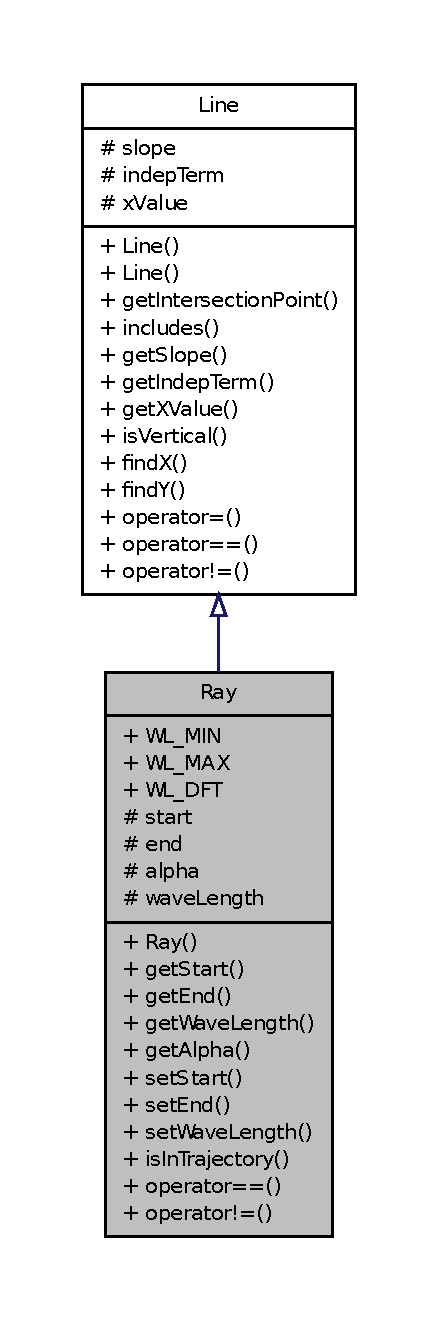
\includegraphics[height=550pt]{da/db5/classRay__inherit__graph}
\end{center}
\end{figure}


Graphe de collaboration de Ray\+:\nopagebreak
\begin{figure}[H]
\begin{center}
\leavevmode
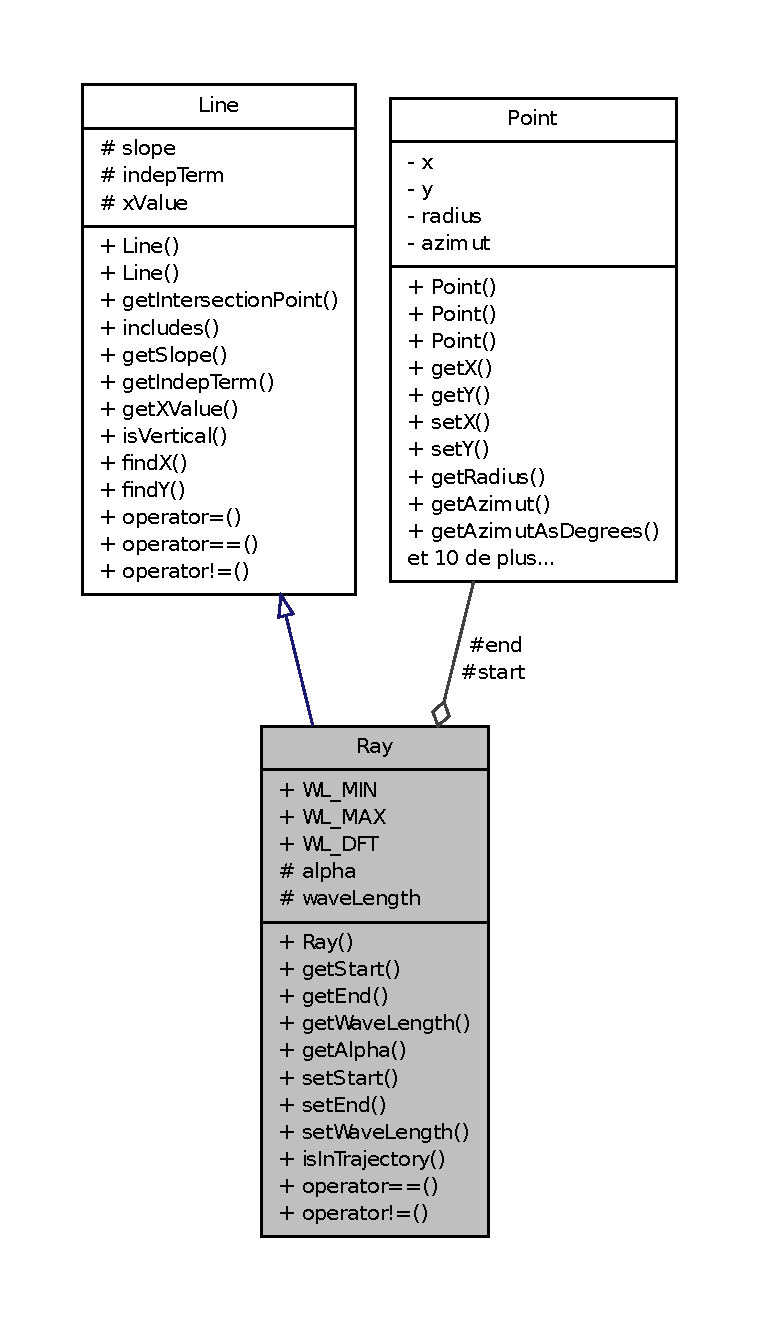
\includegraphics[height=550pt]{db/d2b/classRay__coll__graph}
\end{center}
\end{figure}


\subsection{Documentation des constructeurs et destructeur}
\hypertarget{classRay_af80c80c8ccb7721d3c8a0745ada767fa}{}\index{Ray@{Ray}!Ray@{Ray}}
\index{Ray@{Ray}!Ray@{Ray}}
\subsubsection[{Ray(const Point, double, int=\+Ray\+::\+W\+L\+\_\+\+D\+F\+T)}]{\setlength{\rightskip}{0pt plus 5cm}Ray\+::\+Ray (
\begin{DoxyParamCaption}
\item[{const {\bf Point}}]{, }
\item[{double}]{, }
\item[{int}]{ = {\ttfamily {\bf Ray\+::\+W\+L\+\_\+\+D\+F\+T}}}
\end{DoxyParamCaption}
)}\label{classRay_af80c80c8ccb7721d3c8a0745ada767fa}


Créer un nouveau rayon. 



\subsection{Documentation des fonctions membres}
\hypertarget{classRay_adc4be184293831177b663260619edd37}{}\index{Ray@{Ray}!get\+Alpha@{get\+Alpha}}
\index{get\+Alpha@{get\+Alpha}!Ray@{Ray}}
\subsubsection[{get\+Alpha() const }]{\setlength{\rightskip}{0pt plus 5cm}double Ray\+::get\+Alpha (
\begin{DoxyParamCaption}
{}
\end{DoxyParamCaption}
) const\hspace{0.3cm}{\ttfamily [inline]}}\label{classRay_adc4be184293831177b663260619edd37}


Permet de connaitre l\textquotesingle{}angle du rayon. 

\begin{DoxyReturn}{Renvoie}
L\textquotesingle{}angle du rayon courant. 
\end{DoxyReturn}


Définition à la ligne 169 du fichier ray.\+hpp.



Références alpha.


\begin{DoxyCode}
170 \{
171     \textcolor{keywordflow}{return} this->\hyperlink{classRay_a8660ea53da0f47170387278c127e92ad}{alpha};
172 \}
\end{DoxyCode}
\hypertarget{classRay_a464697d88415597f098d4f34b0fe16b4}{}\index{Ray@{Ray}!get\+End@{get\+End}}
\index{get\+End@{get\+End}!Ray@{Ray}}
\subsubsection[{get\+End() const }]{\setlength{\rightskip}{0pt plus 5cm}const {\bf Point} \& Ray\+::get\+End (
\begin{DoxyParamCaption}
{}
\end{DoxyParamCaption}
) const\hspace{0.3cm}{\ttfamily [inline]}}\label{classRay_a464697d88415597f098d4f34b0fe16b4}


Retourne la fin du rayon. 

\begin{DoxyReturn}{Renvoie}
la fin du rayon. 
\end{DoxyReturn}


Définition à la ligne 159 du fichier ray.\+hpp.



Références end.


\begin{DoxyCode}
160 \{
161     \textcolor{keywordflow}{return} this->\hyperlink{classRay_aceb35dc199d12219c6990ca03627dc43}{end};
162 \}
\end{DoxyCode}
\hypertarget{classRay_a910d5b44324b73c5fa032c24093d4024}{}\index{Ray@{Ray}!get\+Start@{get\+Start}}
\index{get\+Start@{get\+Start}!Ray@{Ray}}
\subsubsection[{get\+Start() const }]{\setlength{\rightskip}{0pt plus 5cm}const {\bf Point} \& Ray\+::get\+Start (
\begin{DoxyParamCaption}
{}
\end{DoxyParamCaption}
) const\hspace{0.3cm}{\ttfamily [inline]}}\label{classRay_a910d5b44324b73c5fa032c24093d4024}


Retourne le début du rayon. 

\begin{DoxyReturn}{Renvoie}
le début du rayon. 
\end{DoxyReturn}


Définition à la ligne 154 du fichier ray.\+hpp.



Références start.


\begin{DoxyCode}
155 \{
156     \textcolor{keywordflow}{return} this->\hyperlink{classRay_a15f35dc363823ce843f4d87e9e0083b9}{start};
157 \}
\end{DoxyCode}
\hypertarget{classRay_a19c018dc962281e70a1a00bf336ad1a4}{}\index{Ray@{Ray}!get\+Wave\+Length@{get\+Wave\+Length}}
\index{get\+Wave\+Length@{get\+Wave\+Length}!Ray@{Ray}}
\subsubsection[{get\+Wave\+Length() const }]{\setlength{\rightskip}{0pt plus 5cm}int Ray\+::get\+Wave\+Length (
\begin{DoxyParamCaption}
{}
\end{DoxyParamCaption}
) const\hspace{0.3cm}{\ttfamily [inline]}}\label{classRay_a19c018dc962281e70a1a00bf336ad1a4}


Retourne la longueur d\textquotesingle{}onde du rayon. 

\begin{DoxyReturn}{Renvoie}
la longueur d\textquotesingle{}onde du rayon. 
\end{DoxyReturn}


Définition à la ligne 164 du fichier ray.\+hpp.



Références wave\+Length.


\begin{DoxyCode}
165 \{
166     \textcolor{keywordflow}{return} this->\hyperlink{classRay_aaa9ec19c151d6ad78d0d0b643b4940df}{waveLength};
167 \}
\end{DoxyCode}
\hypertarget{classRay_a011572c6f75a3bf6fcf0f5d14636d829}{}\index{Ray@{Ray}!is\+In\+Trajectory@{is\+In\+Trajectory}}
\index{is\+In\+Trajectory@{is\+In\+Trajectory}!Ray@{Ray}}
\subsubsection[{is\+In\+Trajectory(const Point \&) const }]{\setlength{\rightskip}{0pt plus 5cm}bool Ray\+::is\+In\+Trajectory (
\begin{DoxyParamCaption}
\item[{const {\bf Point} \&}]{}
\end{DoxyParamCaption}
) const}\label{classRay_a011572c6f75a3bf6fcf0f5d14636d829}


Cette méthode permet de savoir si le point passé en paramètre est bien dans la trajectoire du rayon courant à l\textquotesingle{}aide de la représentation polaire des points. 

\begin{DoxyReturn}{Renvoie}
{\ttfamily true} si le point passé en paramètre est dans la trajectoire. 
\end{DoxyReturn}
\hypertarget{classRay_af4481fb5fdefb9ac5e1572f458bb14e9}{}\index{Ray@{Ray}!operator"!=@{operator"!=}}
\index{operator"!=@{operator"!=}!Ray@{Ray}}
\subsubsection[{operator"!=(const Ray \&) const }]{\setlength{\rightskip}{0pt plus 5cm}bool Ray\+::operator!= (
\begin{DoxyParamCaption}
\item[{const {\bf Ray} \&}]{}
\end{DoxyParamCaption}
) const}\label{classRay_af4481fb5fdefb9ac5e1572f458bb14e9}


Permet de savoir si deux rayons sont différents. 

\begin{DoxyReturn}{Renvoie}
{\ttfamily true} Si deux rayons sont différents. 
\end{DoxyReturn}
\hypertarget{classRay_abdb7998a61b33ea144e6113b2e361081}{}\index{Ray@{Ray}!operator==@{operator==}}
\index{operator==@{operator==}!Ray@{Ray}}
\subsubsection[{operator==(const Ray \&) const }]{\setlength{\rightskip}{0pt plus 5cm}bool Ray\+::operator== (
\begin{DoxyParamCaption}
\item[{const {\bf Ray} \&}]{}
\end{DoxyParamCaption}
) const}\label{classRay_abdb7998a61b33ea144e6113b2e361081}


Permet de savoir si deux rayons sont les mêmes. 

\begin{DoxyReturn}{Renvoie}
{\ttfamily true} Si deux rayons sont les même. 
\end{DoxyReturn}
\hypertarget{classRay_aeebe4e189ed7171473ebd356fb850f63}{}\index{Ray@{Ray}!set\+End@{set\+End}}
\index{set\+End@{set\+End}!Ray@{Ray}}
\subsubsection[{set\+End(const Point \&)}]{\setlength{\rightskip}{0pt plus 5cm}void Ray\+::set\+End (
\begin{DoxyParamCaption}
\item[{const {\bf Point} \&}]{}
\end{DoxyParamCaption}
)}\label{classRay_aeebe4e189ed7171473ebd356fb850f63}


hange la coordonnée de la fin du rayon. 


\begin{DoxyParams}{Paramètres}
{\em end} & La nouvelle coordonnée de la fin du rayon. \\
\hline
\end{DoxyParams}
\hypertarget{classRay_ae329146aa527a3f7b403a818e61f38b7}{}\index{Ray@{Ray}!set\+Start@{set\+Start}}
\index{set\+Start@{set\+Start}!Ray@{Ray}}
\subsubsection[{set\+Start(const Point \&)}]{\setlength{\rightskip}{0pt plus 5cm}void Ray\+::set\+Start (
\begin{DoxyParamCaption}
\item[{const {\bf Point} \&}]{}
\end{DoxyParamCaption}
)}\label{classRay_ae329146aa527a3f7b403a818e61f38b7}


Change la coordonnée du début du rayon. 


\begin{DoxyParams}{Paramètres}
{\em start} & La nouvelle coordonnée du début du rayon. \\
\hline
\end{DoxyParams}
\hypertarget{classRay_ae270a15e468c912d435273576830ef0b}{}\index{Ray@{Ray}!set\+Wave\+Length@{set\+Wave\+Length}}
\index{set\+Wave\+Length@{set\+Wave\+Length}!Ray@{Ray}}
\subsubsection[{set\+Wave\+Length(const int)}]{\setlength{\rightskip}{0pt plus 5cm}void Ray\+::set\+Wave\+Length (
\begin{DoxyParamCaption}
\item[{const int}]{}
\end{DoxyParamCaption}
)}\label{classRay_ae270a15e468c912d435273576830ef0b}


hange la longueur d\textquotesingle{}onde du rayon. 

Si la longueur d\textquotesingle{}onde spécifiée est en dehors des limites autorisées, la longueur d\textquotesingle{}onde vaudra la borne la plus proche. La longueur d\textquotesingle{}onde doit être comprise entre 360 et 830 nm.


\begin{DoxyParams}{Paramètres}
{\em wave\+Length} & La nouvelle longueur d\textquotesingle{}onde du rayon \\
\hline
\end{DoxyParams}


\subsection{Documentation des données membres}
\hypertarget{classRay_a8660ea53da0f47170387278c127e92ad}{}\index{Ray@{Ray}!alpha@{alpha}}
\index{alpha@{alpha}!Ray@{Ray}}
\subsubsection[{alpha}]{\setlength{\rightskip}{0pt plus 5cm}double Ray\+::alpha\hspace{0.3cm}{\ttfamily [protected]}}\label{classRay_a8660ea53da0f47170387278c127e92ad}


L\textquotesingle{}angle de tir du rayon selon le cercle trigonométrique usuel. 



Définition à la ligne 33 du fichier ray.\+hpp.



Référencé par get\+Alpha().

\hypertarget{classRay_aceb35dc199d12219c6990ca03627dc43}{}\index{Ray@{Ray}!end@{end}}
\index{end@{end}!Ray@{Ray}}
\subsubsection[{end}]{\setlength{\rightskip}{0pt plus 5cm}{\bf Point} Ray\+::end\hspace{0.3cm}{\ttfamily [protected]}}\label{classRay_aceb35dc199d12219c6990ca03627dc43}


Le point d\textquotesingle{}arrivé du segment de droite représentant le rayon. 



Définition à la ligne 28 du fichier ray.\+hpp.



Référencé par get\+End().

\hypertarget{classRay_a15f35dc363823ce843f4d87e9e0083b9}{}\index{Ray@{Ray}!start@{start}}
\index{start@{start}!Ray@{Ray}}
\subsubsection[{start}]{\setlength{\rightskip}{0pt plus 5cm}{\bf Point} Ray\+::start\hspace{0.3cm}{\ttfamily [protected]}}\label{classRay_a15f35dc363823ce843f4d87e9e0083b9}


Le point de départ du segment de droite représentant le rayon. 



Définition à la ligne 23 du fichier ray.\+hpp.



Référencé par get\+Start().

\hypertarget{classRay_aaa9ec19c151d6ad78d0d0b643b4940df}{}\index{Ray@{Ray}!wave\+Length@{wave\+Length}}
\index{wave\+Length@{wave\+Length}!Ray@{Ray}}
\subsubsection[{wave\+Length}]{\setlength{\rightskip}{0pt plus 5cm}int Ray\+::wave\+Length\hspace{0.3cm}{\ttfamily [protected]}}\label{classRay_aaa9ec19c151d6ad78d0d0b643b4940df}


La longueur d\textquotesingle{}onde du rayon. 



Définition à la ligne 38 du fichier ray.\+hpp.



Référencé par get\+Wave\+Length().

\hypertarget{classRay_af4176c69ef62ea83bf84b40d7e1c5560}{}\index{Ray@{Ray}!W\+L\+\_\+\+D\+F\+T@{W\+L\+\_\+\+D\+F\+T}}
\index{W\+L\+\_\+\+D\+F\+T@{W\+L\+\_\+\+D\+F\+T}!Ray@{Ray}}
\subsubsection[{W\+L\+\_\+\+D\+F\+T}]{\setlength{\rightskip}{0pt plus 5cm}const int Ray\+::\+W\+L\+\_\+\+D\+F\+T \{600\}\hspace{0.3cm}{\ttfamily [static]}}\label{classRay_af4176c69ef62ea83bf84b40d7e1c5560}


Longueur d\textquotesingle{}onde par défaut pour un rayon lumineux. 

Cette valeur correspond à la longueur d\textquotesingle{}onde (en nm) de la couleur orangé-\/rouge du spectre visible de la lumière. 

Définition à la ligne 61 du fichier ray.\+hpp.

\hypertarget{classRay_add278b4978966f54e3c22e8be2224b7f}{}\index{Ray@{Ray}!W\+L\+\_\+\+M\+A\+X@{W\+L\+\_\+\+M\+A\+X}}
\index{W\+L\+\_\+\+M\+A\+X@{W\+L\+\_\+\+M\+A\+X}!Ray@{Ray}}
\subsubsection[{W\+L\+\_\+\+M\+A\+X}]{\setlength{\rightskip}{0pt plus 5cm}const int Ray\+::\+W\+L\+\_\+\+M\+A\+X \{830\}\hspace{0.3cm}{\ttfamily [static]}}\label{classRay_add278b4978966f54e3c22e8be2224b7f}


Longueur d\textquotesingle{}onde maximum autorisée pour un rayon lumineux. 

Cette valeur correspond à la longueur d\textquotesingle{}onde maximum (en nm) du spectre visible de la lumière. 

Définition à la ligne 54 du fichier ray.\+hpp.

\hypertarget{classRay_a478177dabc9f1a3a0ba7d8b388a58b7e}{}\index{Ray@{Ray}!W\+L\+\_\+\+M\+I\+N@{W\+L\+\_\+\+M\+I\+N}}
\index{W\+L\+\_\+\+M\+I\+N@{W\+L\+\_\+\+M\+I\+N}!Ray@{Ray}}
\subsubsection[{W\+L\+\_\+\+M\+I\+N}]{\setlength{\rightskip}{0pt plus 5cm}const int Ray\+::\+W\+L\+\_\+\+M\+I\+N \{360\}\hspace{0.3cm}{\ttfamily [static]}}\label{classRay_a478177dabc9f1a3a0ba7d8b388a58b7e}


Longueur d\textquotesingle{}onde minimum autorisée pour un rayon lumineux. 

Cette valeur correspond à la longueur d\textquotesingle{}onde minimum (en nm) du spectre visible de la lumière. 

Définition à la ligne 47 du fichier ray.\+hpp.



La documentation de cette classe a été générée à partir du fichier suivant \+:\begin{DoxyCompactItemize}
\item 
model/elements/\hyperlink{ray_8hpp}{ray.\+hpp}\end{DoxyCompactItemize}

\hypertarget{classRectangle}{}\section{Référence de la classe Rectangle}
\label{classRectangle}\index{Rectangle@{Rectangle}}


Le rectangle est objet géométrique, du plan, à quatre coté parallèles deux à deux.  




{\ttfamily \#include $<$rectangle.\+hpp$>$}

\subsection*{Fonctions membres publiques}
\begin{DoxyCompactItemize}
\item 
\hyperlink{classRectangle_ad5508555707c9e4d7334292a08037079}{Rectangle} (double, double, const \hyperlink{classPoint}{Point} \&)
\begin{DoxyCompactList}\small\item\em Permet de construire un nouveau rectangle initialisé. \end{DoxyCompactList}\item 
std\+::vector$<$ \hyperlink{classPoint}{Point} $>$ \hyperlink{classRectangle_a062fb917aa2d811e17ed59caa43c662a}{get\+Intersection\+Points} (const \hyperlink{classLine}{Line} \&) const 
\begin{DoxyCompactList}\small\item\em Permet d\textquotesingle{}obtenir les points d\textquotesingle{}intersection entre le rectangle et la droite entrée en paramètre. \end{DoxyCompactList}\item 
bool \hyperlink{classRectangle_a74f9fcc2cd8e170fd13137b95903dcb5}{is\+On\+Border} (const \hyperlink{classPoint}{Point} \&) const 
\begin{DoxyCompactList}\small\item\em Renseigne si un point se trouve sur la bordure du rectangle. \end{DoxyCompactList}\item 
std\+::vector$<$ \hyperlink{classLine}{Line} $>$ \hyperlink{classRectangle_aaed6939da22aef8b1028b3310c4b0ff0}{get\+Edges} () const 
\begin{DoxyCompactList}\small\item\em Permet d\textquotesingle{}obtenir les côtés du rectangle sous forme de droites. \end{DoxyCompactList}\item 
virtual double \hyperlink{classRectangle_a1b97d538cc1acefa6b09aae2160e7921}{get\+Width} () const 
\begin{DoxyCompactList}\small\item\em Permet d\textquotesingle{}obtenir la longueur du rectangle. \end{DoxyCompactList}\item 
virtual double \hyperlink{classRectangle_aaad99f5dd2be859eef0eb3482cb55c13}{get\+Height} () const 
\begin{DoxyCompactList}\small\item\em Permet d\textquotesingle{}obtenir la hauteur du rectangle. \end{DoxyCompactList}\item 
\hyperlink{classPoint}{Point} \hyperlink{classRectangle_af54d3160a6d8d6c432b547207d997052}{get\+Up\+Left\+Corner} () const 
\begin{DoxyCompactList}\small\item\em Permet d\textquotesingle{}obtenir les coordonnées du coté supérieur du rectangle. \end{DoxyCompactList}\item 
bool \hyperlink{classRectangle_a140aa8d43ff12d36f3891dea9f439638}{operator==} (const \hyperlink{classRectangle}{Rectangle} \&) const 
\begin{DoxyCompactList}\small\item\em Permet de savoir si deux rectangles sont identiques. \end{DoxyCompactList}\item 
bool \hyperlink{classRectangle_ac29d68cce7f438771cf2b0e72888457a}{operator!=} (const \hyperlink{classRectangle}{Rectangle} \&) const 
\begin{DoxyCompactList}\small\item\em Permet de savoir si deux rectangles sont différents. \end{DoxyCompactList}\item 
\hyperlink{classRectangle}{Rectangle} \& \hyperlink{classRectangle_a64aa28fe918b233e6241a7841465b093}{operator=} (const \hyperlink{classRectangle}{Rectangle} \&)
\begin{DoxyCompactList}\small\item\em Permet de copier un rectangle dans un autre. \end{DoxyCompactList}\end{DoxyCompactItemize}
\subsection*{Attributs protégés}
\begin{DoxyCompactItemize}
\item 
double \hyperlink{classRectangle_ac2c47512ca05c56cec73c32bb693d479}{width}
\begin{DoxyCompactList}\small\item\em La largeur du rectangle. \end{DoxyCompactList}\item 
double \hyperlink{classRectangle_a58c0573f0d706d238759395e8272c6bf}{height}
\begin{DoxyCompactList}\small\item\em La longueur du rectangle. \end{DoxyCompactList}\item 
\hyperlink{classPoint}{Point} \hyperlink{classRectangle_aeeb6ca62aa27e964265c92d1ea25d511}{up\+Left\+Corner}
\begin{DoxyCompactList}\small\item\em La position du coin supérieur gauche du rectangle. \end{DoxyCompactList}\item 
std\+::vector$<$ \hyperlink{classLine}{Line} $>$ \hyperlink{classRectangle_a2c04232970a644df46826a411714966f}{edges}
\begin{DoxyCompactList}\small\item\em Les équations des 4 droites composant le rectangle. \end{DoxyCompactList}\end{DoxyCompactItemize}


\subsection{Description détaillée}
Le rectangle est objet géométrique, du plan, à quatre coté parallèles deux à deux. 

Définition à la ligne 14 du fichier rectangle.\+hpp.



Graphe d\textquotesingle{}héritage de Rectangle\+:\nopagebreak
\begin{figure}[H]
\begin{center}
\leavevmode
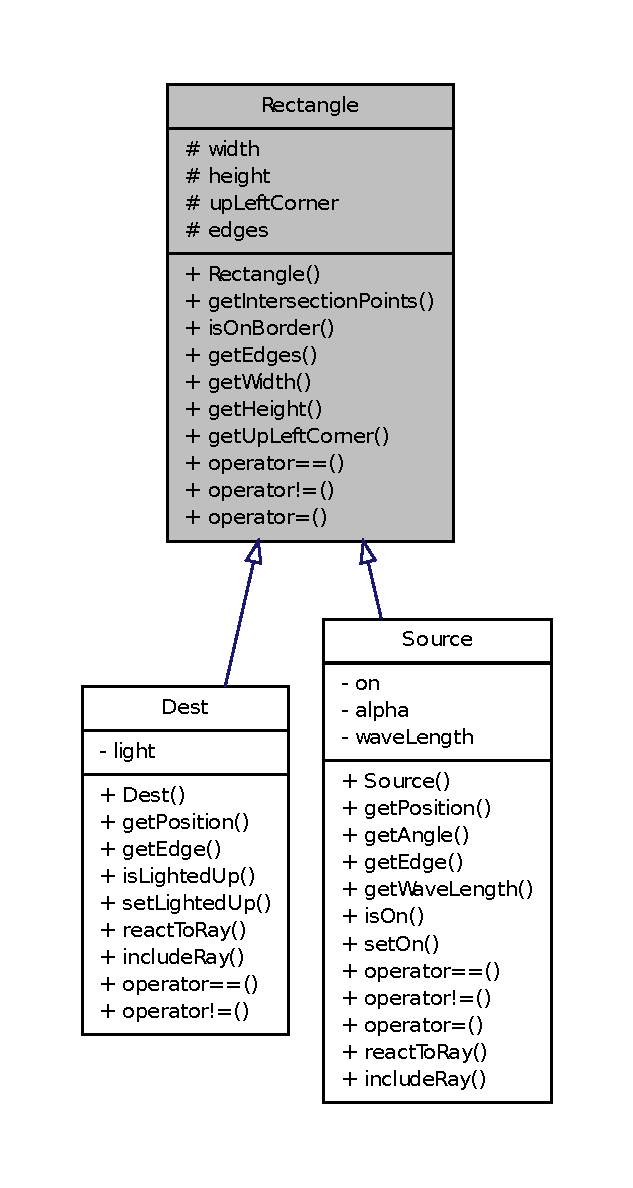
\includegraphics[height=550pt]{dd/d23/classRectangle__inherit__graph}
\end{center}
\end{figure}


Graphe de collaboration de Rectangle\+:\nopagebreak
\begin{figure}[H]
\begin{center}
\leavevmode
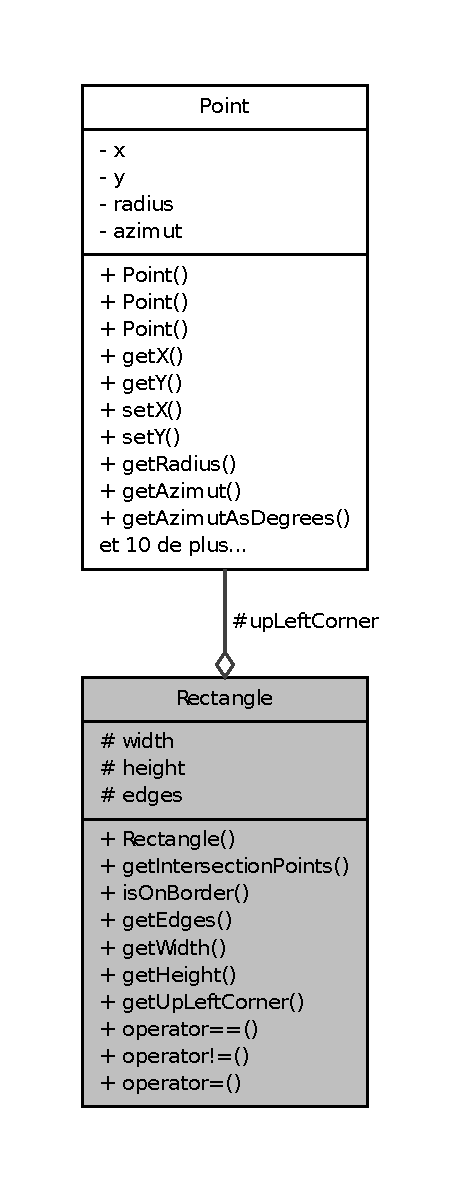
\includegraphics[height=550pt]{db/dea/classRectangle__coll__graph}
\end{center}
\end{figure}


\subsection{Documentation des constructeurs et destructeur}
\hypertarget{classRectangle_ad5508555707c9e4d7334292a08037079}{}\index{Rectangle@{Rectangle}!Rectangle@{Rectangle}}
\index{Rectangle@{Rectangle}!Rectangle@{Rectangle}}
\subsubsection[{Rectangle(double, double, const Point \&)}]{\setlength{\rightskip}{0pt plus 5cm}Rectangle\+::\+Rectangle (
\begin{DoxyParamCaption}
\item[{double}]{, }
\item[{double}]{, }
\item[{const {\bf Point} \&}]{}
\end{DoxyParamCaption}
)}\label{classRectangle_ad5508555707c9e4d7334292a08037079}


Permet de construire un nouveau rectangle initialisé. 


\begin{DoxyParams}{Paramètres}
{\em width} & Largeur du rectangle. \\
\hline
{\em height} & Hauteur du rectangle. \\
\hline
{\em up\+Left\+Corner} & Côté supérieur gauche du rectangle. \\
\hline
\end{DoxyParams}


\subsection{Documentation des fonctions membres}
\hypertarget{classRectangle_aaed6939da22aef8b1028b3310c4b0ff0}{}\index{Rectangle@{Rectangle}!get\+Edges@{get\+Edges}}
\index{get\+Edges@{get\+Edges}!Rectangle@{Rectangle}}
\subsubsection[{get\+Edges() const }]{\setlength{\rightskip}{0pt plus 5cm}std\+::vector$<$ {\bf Line} $>$ Rectangle\+::get\+Edges (
\begin{DoxyParamCaption}
{}
\end{DoxyParamCaption}
) const\hspace{0.3cm}{\ttfamily [inline]}}\label{classRectangle_aaed6939da22aef8b1028b3310c4b0ff0}


Permet d\textquotesingle{}obtenir les côtés du rectangle sous forme de droites. 

\begin{DoxyReturn}{Renvoie}
Les côtés du rectangle sous forme de droites. 
\end{DoxyReturn}


Définition à la ligne 132 du fichier rectangle.\+hpp.



Références edges.


\begin{DoxyCode}
133 \{
134     \textcolor{keywordflow}{return} this->\hyperlink{classRectangle_a2c04232970a644df46826a411714966f}{edges};
135 \}
\end{DoxyCode}
\hypertarget{classRectangle_aaad99f5dd2be859eef0eb3482cb55c13}{}\index{Rectangle@{Rectangle}!get\+Height@{get\+Height}}
\index{get\+Height@{get\+Height}!Rectangle@{Rectangle}}
\subsubsection[{get\+Height() const }]{\setlength{\rightskip}{0pt plus 5cm}double Rectangle\+::get\+Height (
\begin{DoxyParamCaption}
{}
\end{DoxyParamCaption}
) const\hspace{0.3cm}{\ttfamily [inline]}, {\ttfamily [virtual]}}\label{classRectangle_aaad99f5dd2be859eef0eb3482cb55c13}


Permet d\textquotesingle{}obtenir la hauteur du rectangle. 

\begin{DoxyReturn}{Renvoie}
La hauteur du rectangle. 
\end{DoxyReturn}


Définition à la ligne 142 du fichier rectangle.\+hpp.



Références height.


\begin{DoxyCode}
143 \{
144     \textcolor{keywordflow}{return} this->\hyperlink{classRectangle_a58c0573f0d706d238759395e8272c6bf}{height};
145 \}
\end{DoxyCode}
\hypertarget{classRectangle_a062fb917aa2d811e17ed59caa43c662a}{}\index{Rectangle@{Rectangle}!get\+Intersection\+Points@{get\+Intersection\+Points}}
\index{get\+Intersection\+Points@{get\+Intersection\+Points}!Rectangle@{Rectangle}}
\subsubsection[{get\+Intersection\+Points(const Line \&) const }]{\setlength{\rightskip}{0pt plus 5cm}std\+::vector$<${\bf Point}$>$ Rectangle\+::get\+Intersection\+Points (
\begin{DoxyParamCaption}
\item[{const {\bf Line} \&}]{}
\end{DoxyParamCaption}
) const}\label{classRectangle_a062fb917aa2d811e17ed59caa43c662a}


Permet d\textquotesingle{}obtenir les points d\textquotesingle{}intersection entre le rectangle et la droite entrée en paramètre. 


\begin{DoxyParams}{Paramètres}
{\em line} & Droite dont on désire obtenir le point d\textquotesingle{}intersection avec la droite courante.\\
\hline
\end{DoxyParams}
\begin{DoxyReturn}{Renvoie}
Un vecteur contenant les points d\textquotesingle{}intersection entre la droite entrée en paramètre et le rectangle. 
\end{DoxyReturn}
\hypertarget{classRectangle_af54d3160a6d8d6c432b547207d997052}{}\index{Rectangle@{Rectangle}!get\+Up\+Left\+Corner@{get\+Up\+Left\+Corner}}
\index{get\+Up\+Left\+Corner@{get\+Up\+Left\+Corner}!Rectangle@{Rectangle}}
\subsubsection[{get\+Up\+Left\+Corner() const }]{\setlength{\rightskip}{0pt plus 5cm}{\bf Point} Rectangle\+::get\+Up\+Left\+Corner (
\begin{DoxyParamCaption}
{}
\end{DoxyParamCaption}
) const\hspace{0.3cm}{\ttfamily [inline]}}\label{classRectangle_af54d3160a6d8d6c432b547207d997052}


Permet d\textquotesingle{}obtenir les coordonnées du coté supérieur du rectangle. 

\begin{DoxyReturn}{Renvoie}
Les coordonnées du coté supérieur du rectangle. 
\end{DoxyReturn}


Définition à la ligne 147 du fichier rectangle.\+hpp.



Références up\+Left\+Corner.


\begin{DoxyCode}
148 \{
149     \textcolor{keywordflow}{return} this->\hyperlink{classRectangle_aeeb6ca62aa27e964265c92d1ea25d511}{upLeftCorner};
150 \}
\end{DoxyCode}
\hypertarget{classRectangle_a1b97d538cc1acefa6b09aae2160e7921}{}\index{Rectangle@{Rectangle}!get\+Width@{get\+Width}}
\index{get\+Width@{get\+Width}!Rectangle@{Rectangle}}
\subsubsection[{get\+Width() const }]{\setlength{\rightskip}{0pt plus 5cm}double Rectangle\+::get\+Width (
\begin{DoxyParamCaption}
{}
\end{DoxyParamCaption}
) const\hspace{0.3cm}{\ttfamily [inline]}, {\ttfamily [virtual]}}\label{classRectangle_a1b97d538cc1acefa6b09aae2160e7921}


Permet d\textquotesingle{}obtenir la longueur du rectangle. 

\begin{DoxyReturn}{Renvoie}
La longueur du rectangle. 
\end{DoxyReturn}


Définition à la ligne 137 du fichier rectangle.\+hpp.



Références width.


\begin{DoxyCode}
138 \{
139     \textcolor{keywordflow}{return} this->\hyperlink{classRectangle_ac2c47512ca05c56cec73c32bb693d479}{width};
140 \}
\end{DoxyCode}
\hypertarget{classRectangle_a74f9fcc2cd8e170fd13137b95903dcb5}{}\index{Rectangle@{Rectangle}!is\+On\+Border@{is\+On\+Border}}
\index{is\+On\+Border@{is\+On\+Border}!Rectangle@{Rectangle}}
\subsubsection[{is\+On\+Border(const Point \&) const }]{\setlength{\rightskip}{0pt plus 5cm}bool Rectangle\+::is\+On\+Border (
\begin{DoxyParamCaption}
\item[{const {\bf Point} \&}]{}
\end{DoxyParamCaption}
) const}\label{classRectangle_a74f9fcc2cd8e170fd13137b95903dcb5}


Renseigne si un point se trouve sur la bordure du rectangle. 


\begin{DoxyParams}{Paramètres}
{\em point} & \hyperlink{classPoint}{Point} dont on désire savoir s\textquotesingle{}il est inclus sur la bordure du rectangle.\\
\hline
\end{DoxyParams}
\begin{DoxyReturn}{Renvoie}
{\ttfamily true} Si le \hyperlink{classPoint}{Point} entré en paramètre est inclus sur la bordure du rectangle. 
\end{DoxyReturn}
\hypertarget{classRectangle_ac29d68cce7f438771cf2b0e72888457a}{}\index{Rectangle@{Rectangle}!operator"!=@{operator"!=}}
\index{operator"!=@{operator"!=}!Rectangle@{Rectangle}}
\subsubsection[{operator"!=(const Rectangle \&) const }]{\setlength{\rightskip}{0pt plus 5cm}bool Rectangle\+::operator!= (
\begin{DoxyParamCaption}
\item[{const {\bf Rectangle} \&}]{}
\end{DoxyParamCaption}
) const}\label{classRectangle_ac29d68cce7f438771cf2b0e72888457a}


Permet de savoir si deux rectangles sont différents. 

\begin{DoxyReturn}{Renvoie}
{\ttfamily true} Si les deux rectangles sont différents. 
\end{DoxyReturn}
\hypertarget{classRectangle_a64aa28fe918b233e6241a7841465b093}{}\index{Rectangle@{Rectangle}!operator=@{operator=}}
\index{operator=@{operator=}!Rectangle@{Rectangle}}
\subsubsection[{operator=(const Rectangle \&)}]{\setlength{\rightskip}{0pt plus 5cm}{\bf Rectangle}\& Rectangle\+::operator= (
\begin{DoxyParamCaption}
\item[{const {\bf Rectangle} \&}]{}
\end{DoxyParamCaption}
)}\label{classRectangle_a64aa28fe918b233e6241a7841465b093}


Permet de copier un rectangle dans un autre. 

\begin{DoxyReturn}{Renvoie}
Le rectangle courant modifié. 
\end{DoxyReturn}
\hypertarget{classRectangle_a140aa8d43ff12d36f3891dea9f439638}{}\index{Rectangle@{Rectangle}!operator==@{operator==}}
\index{operator==@{operator==}!Rectangle@{Rectangle}}
\subsubsection[{operator==(const Rectangle \&) const }]{\setlength{\rightskip}{0pt plus 5cm}bool Rectangle\+::operator== (
\begin{DoxyParamCaption}
\item[{const {\bf Rectangle} \&}]{}
\end{DoxyParamCaption}
) const}\label{classRectangle_a140aa8d43ff12d36f3891dea9f439638}


Permet de savoir si deux rectangles sont identiques. 

\begin{DoxyReturn}{Renvoie}
{\ttfamily true} Si les deux rectangles sont identiques. 
\end{DoxyReturn}


\subsection{Documentation des données membres}
\hypertarget{classRectangle_a2c04232970a644df46826a411714966f}{}\index{Rectangle@{Rectangle}!edges@{edges}}
\index{edges@{edges}!Rectangle@{Rectangle}}
\subsubsection[{edges}]{\setlength{\rightskip}{0pt plus 5cm}std\+::vector$<${\bf Line}$>$ Rectangle\+::edges\hspace{0.3cm}{\ttfamily [protected]}}\label{classRectangle_a2c04232970a644df46826a411714966f}


Les équations des 4 droites composant le rectangle. 



Définition à la ligne 37 du fichier rectangle.\+hpp.



Référencé par get\+Edges().

\hypertarget{classRectangle_a58c0573f0d706d238759395e8272c6bf}{}\index{Rectangle@{Rectangle}!height@{height}}
\index{height@{height}!Rectangle@{Rectangle}}
\subsubsection[{height}]{\setlength{\rightskip}{0pt plus 5cm}double Rectangle\+::height\hspace{0.3cm}{\ttfamily [protected]}}\label{classRectangle_a58c0573f0d706d238759395e8272c6bf}


La longueur du rectangle. 



Définition à la ligne 27 du fichier rectangle.\+hpp.



Référencé par Dest\+::get\+Edge(), et get\+Height().

\hypertarget{classRectangle_aeeb6ca62aa27e964265c92d1ea25d511}{}\index{Rectangle@{Rectangle}!up\+Left\+Corner@{up\+Left\+Corner}}
\index{up\+Left\+Corner@{up\+Left\+Corner}!Rectangle@{Rectangle}}
\subsubsection[{up\+Left\+Corner}]{\setlength{\rightskip}{0pt plus 5cm}{\bf Point} Rectangle\+::up\+Left\+Corner\hspace{0.3cm}{\ttfamily [protected]}}\label{classRectangle_aeeb6ca62aa27e964265c92d1ea25d511}


La position du coin supérieur gauche du rectangle. 



Définition à la ligne 32 du fichier rectangle.\+hpp.



Référencé par Dest\+::get\+Position(), Source\+::get\+Position(), et get\+Up\+Left\+Corner().

\hypertarget{classRectangle_ac2c47512ca05c56cec73c32bb693d479}{}\index{Rectangle@{Rectangle}!width@{width}}
\index{width@{width}!Rectangle@{Rectangle}}
\subsubsection[{width}]{\setlength{\rightskip}{0pt plus 5cm}double Rectangle\+::width\hspace{0.3cm}{\ttfamily [protected]}}\label{classRectangle_ac2c47512ca05c56cec73c32bb693d479}


La largeur du rectangle. 



Définition à la ligne 22 du fichier rectangle.\+hpp.



Référencé par Source\+::get\+Edge(), et get\+Width().



La documentation de cette classe a été générée à partir du fichier suivant \+:\begin{DoxyCompactItemize}
\item 
model/geometry/\hyperlink{rectangle_8hpp}{rectangle.\+hpp}\end{DoxyCompactItemize}

\hypertarget{classSource}{}\section{Référence de la classe Source}
\label{classSource}\index{Source@{Source}}


Modélise la source lumineuse utilisée dans le jeu.  




{\ttfamily \#include $<$source.\+hpp$>$}

\subsection*{Fonctions membres publiques}
\begin{DoxyCompactItemize}
\item 
\hyperlink{classSource_a57e5f78dc14db333535f1f83b0c2fb63}{Source} (const \hyperlink{classPoint}{Point} \&, const int, const double, const int)
\begin{DoxyCompactList}\small\item\em Instancie une nouvelle source de position, côté et longueur d\textquotesingle{}onde donnée. \end{DoxyCompactList}\item 
const \hyperlink{classPoint}{Point} \& \hyperlink{classSource_a3a934cb50b20015ed142070893fb9661}{get\+Position} () const 
\begin{DoxyCompactList}\small\item\em Retourne la coordonnée du coin supérieur gauche du carré modélisant la destination. \end{DoxyCompactList}\item 
double \hyperlink{classSource_a8e6f805715dbadf4784dcfcf60b8fb6a}{get\+Angle} () const 
\begin{DoxyCompactList}\small\item\em Retourne l\textquotesingle{}angle du rayon émis. \end{DoxyCompactList}\item 
int \hyperlink{classSource_a0db163e078500dd3fea9bb3b67d832f3}{get\+Edge} () const 
\begin{DoxyCompactList}\small\item\em Retourne la longueur du côté du carré. \end{DoxyCompactList}\item 
int \hyperlink{classSource_ab316229f3514eb474313d87daff6ba26}{get\+Wave\+Length} () const 
\begin{DoxyCompactList}\small\item\em Retourne la longueur d\textquotesingle{}onde du rayon émis. \end{DoxyCompactList}\item 
bool \hyperlink{classSource_ac6ec1663e9a294d6879a7ccc241cbf1b}{is\+On} () const 
\begin{DoxyCompactList}\small\item\em Permet de savoir l\textquotesingle{}état d\textquotesingle{}émission de la source. \end{DoxyCompactList}\item 
void \hyperlink{classSource_aee33db3751f8acde346a713254a5ceea}{set\+On} (const bool)
\begin{DoxyCompactList}\small\item\em Allume ou éteint la source. \end{DoxyCompactList}\item 
bool \hyperlink{classSource_a568cc17208751ca3dc56348b29231f31}{operator==} (const \hyperlink{classSource}{Source} \&) const 
\begin{DoxyCompactList}\small\item\em Permet de savoir si deux sources sont les mêmes. \end{DoxyCompactList}\item 
bool \hyperlink{classSource_a5b02a738eaddd67ede3739a4f8ecd0fe}{operator!=} (const \hyperlink{classSource}{Source} \&) const 
\begin{DoxyCompactList}\small\item\em Permet de savoir si deux sources sont différentes. \end{DoxyCompactList}\item 
\hyperlink{classSource}{Source} \& \hyperlink{classSource_a0b28dc1b1b1a7d125cca3fac3c40083d}{operator=} (const \hyperlink{classSource}{Source} \&)
\begin{DoxyCompactList}\small\item\em Permet de copier la source en paramètre dans la source locale. \end{DoxyCompactList}\item 
void \hyperlink{classSource_a425f400307f756ca8e39e5cfddb3d528}{react\+To\+Ray} (\hyperlink{classRay}{Ray})
\begin{DoxyCompactList}\small\item\em Cette méthode est la réaction de la source face à un rayon. \end{DoxyCompactList}\item 
\hyperlink{classPoint}{Point} $\ast$ \hyperlink{classSource_add4e9c5a8829777d5c522622ad31f431}{include\+Ray} (const \hyperlink{classRay}{Ray} \&) const 
\begin{DoxyCompactList}\small\item\em Cette méthode permet de savoir si la source comprend un point. \end{DoxyCompactList}\end{DoxyCompactItemize}
\subsection*{Attributs privés}
\begin{DoxyCompactItemize}
\item 
bool \hyperlink{classSource_a107c6fed00d6f92226c2e6b9952a28d8}{on}
\begin{DoxyCompactList}\small\item\em État d\textquotesingle{}émission de la source. \end{DoxyCompactList}\item 
double \hyperlink{classSource_a6dc971f9c6ba4291e9d70d622b2425bf}{alpha}
\begin{DoxyCompactList}\small\item\em L\textquotesingle{}angle, en radian, d\textquotesingle{}émission de la source lumineuse. \end{DoxyCompactList}\item 
int \hyperlink{classSource_a1909285fbaf2074d3aee9386a32ebb74}{wave\+Length}
\begin{DoxyCompactList}\small\item\em La longueur d\textquotesingle{}onde du rayon tiré par la source. \end{DoxyCompactList}\end{DoxyCompactItemize}
\subsection*{Membres hérités additionnels}


\subsection{Description détaillée}
Modélise la source lumineuse utilisée dans le jeu. 

La source est un objet carré qui, si allumée, émet un rayon lumineux de longueur d\textquotesingle{}onde donnée dont l\textquotesingle{}angle ne peut pas être changé. Le rayon lumineux est émis depuis la position, i.\+e., le coin supérieur gauche, de la source. 

Définition à la ligne 19 du fichier source.\+hpp.



Graphe d\textquotesingle{}héritage de Source\+:\nopagebreak
\begin{figure}[H]
\begin{center}
\leavevmode
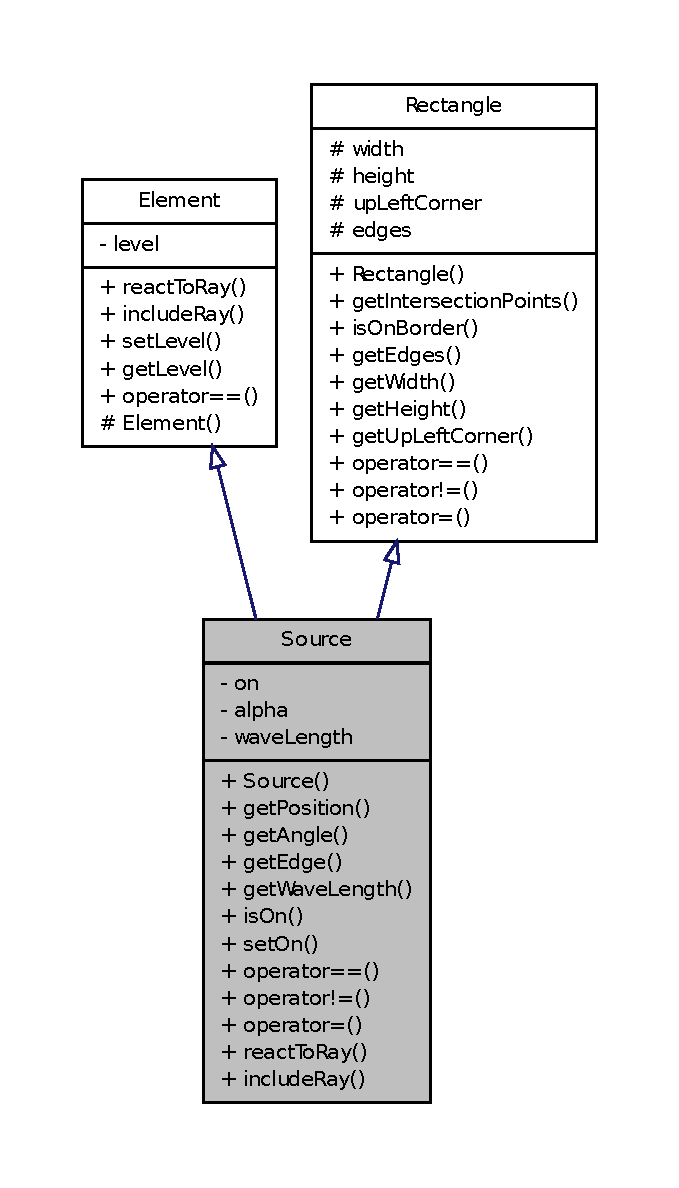
\includegraphics[height=550pt]{da/d95/classSource__inherit__graph}
\end{center}
\end{figure}


Graphe de collaboration de Source\+:\nopagebreak
\begin{figure}[H]
\begin{center}
\leavevmode
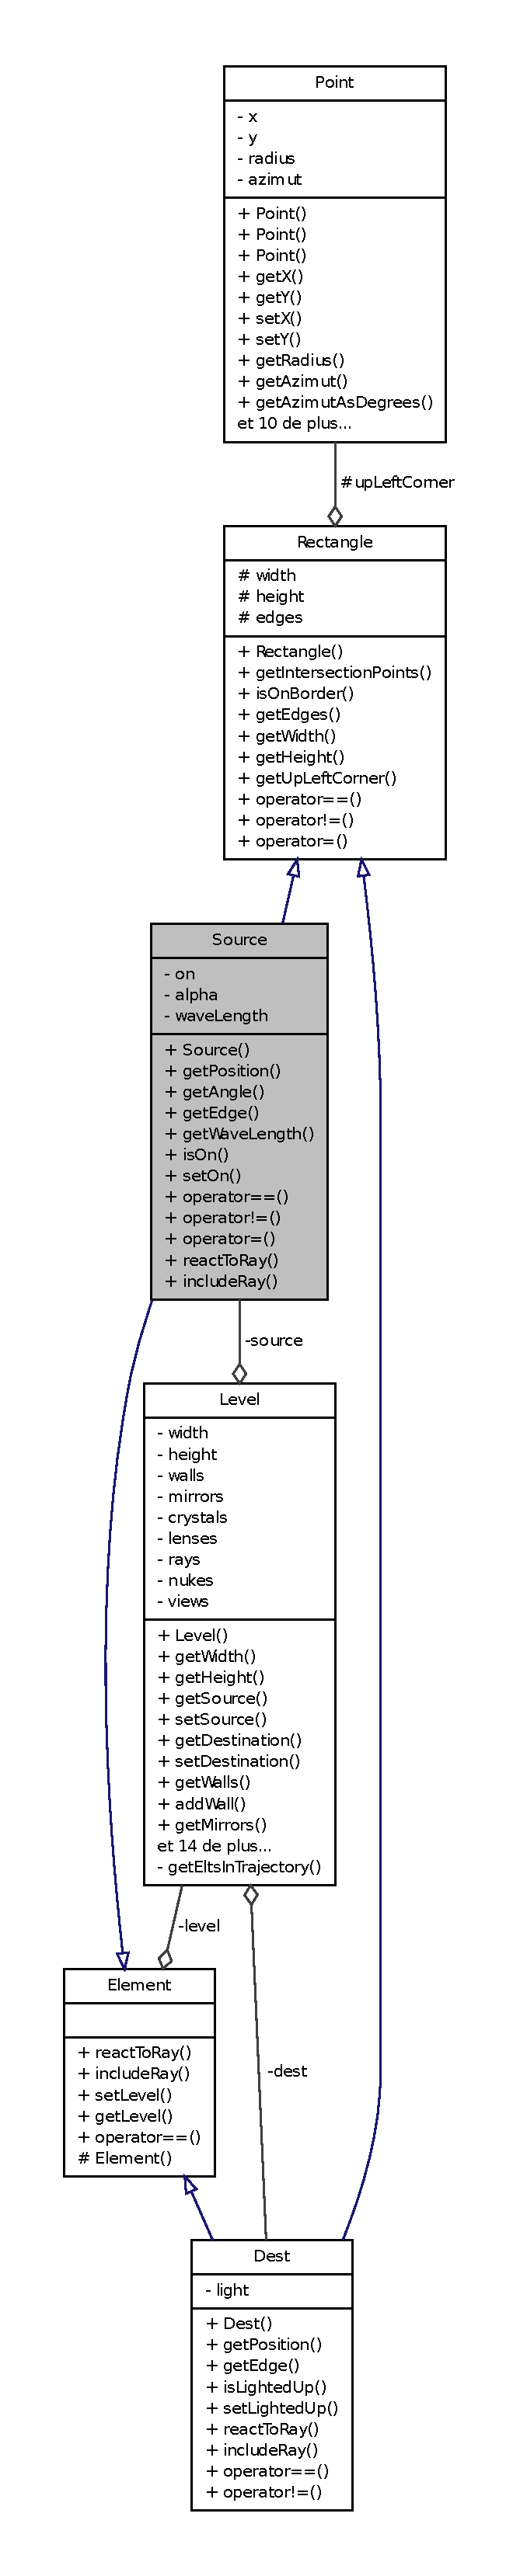
\includegraphics[height=550pt]{d1/d35/classSource__coll__graph}
\end{center}
\end{figure}


\subsection{Documentation des constructeurs et destructeur}
\hypertarget{classSource_a57e5f78dc14db333535f1f83b0c2fb63}{}\index{Source@{Source}!Source@{Source}}
\index{Source@{Source}!Source@{Source}}
\subsubsection[{Source(const Point \&, const int, const double, const int)}]{\setlength{\rightskip}{0pt plus 5cm}Source\+::\+Source (
\begin{DoxyParamCaption}
\item[{const {\bf Point} \&}]{, }
\item[{const int}]{, }
\item[{const double}]{, }
\item[{const int}]{}
\end{DoxyParamCaption}
)}\label{classSource_a57e5f78dc14db333535f1f83b0c2fb63}


Instancie une nouvelle source de position, côté et longueur d\textquotesingle{}onde donnée. 

La position dénote la coordonnée du coin supérieur gauche du carré modélisant la source. La source est initialement éteinte. Si la longueur d\textquotesingle{}onde du rayon lumineux émis n\textquotesingle{}est pas comprise entre 360 nm et 830 nm, elle est réglée sur 600 nm. 
\begin{DoxyParams}{Paramètres}
{\em position} & La position du coin supérieur gauche de la source. \\
\hline
{\em edge} & La longueur du côté du carré modélisant la source. \\
\hline
{\em wave\+Length} & La longueur d\textquotesingle{}onde du rayon lumineux émis.\\
\hline
\end{DoxyParams}
\begin{DoxySeeAlso}{Voir également}
\hyperlink{classRay_a478177dabc9f1a3a0ba7d8b388a58b7e}{Ray\+::\+W\+L\+\_\+\+M\+I\+N} 

\hyperlink{classRay_add278b4978966f54e3c22e8be2224b7f}{Ray\+::\+W\+L\+\_\+\+M\+A\+X} 

\hyperlink{classRay_af4176c69ef62ea83bf84b40d7e1c5560}{Ray\+::\+W\+L\+\_\+\+D\+F\+T} 
\end{DoxySeeAlso}


\subsection{Documentation des fonctions membres}
\hypertarget{classSource_a8e6f805715dbadf4784dcfcf60b8fb6a}{}\index{Source@{Source}!get\+Angle@{get\+Angle}}
\index{get\+Angle@{get\+Angle}!Source@{Source}}
\subsubsection[{get\+Angle() const }]{\setlength{\rightskip}{0pt plus 5cm}double Source\+::get\+Angle (
\begin{DoxyParamCaption}
{}
\end{DoxyParamCaption}
) const\hspace{0.3cm}{\ttfamily [inline]}}\label{classSource_a8e6f805715dbadf4784dcfcf60b8fb6a}


Retourne l\textquotesingle{}angle du rayon émis. 

\begin{DoxyReturn}{Renvoie}
l\textquotesingle{}angle du rayon émis. 
\end{DoxyReturn}


Définition à la ligne 146 du fichier source.\+hpp.



Références alpha.


\begin{DoxyCode}
147 \{
148     \textcolor{keywordflow}{return} this->\hyperlink{classSource_a6dc971f9c6ba4291e9d70d622b2425bf}{alpha};
149 \}
\end{DoxyCode}
\hypertarget{classSource_a0db163e078500dd3fea9bb3b67d832f3}{}\index{Source@{Source}!get\+Edge@{get\+Edge}}
\index{get\+Edge@{get\+Edge}!Source@{Source}}
\subsubsection[{get\+Edge() const }]{\setlength{\rightskip}{0pt plus 5cm}int Source\+::get\+Edge (
\begin{DoxyParamCaption}
{}
\end{DoxyParamCaption}
) const\hspace{0.3cm}{\ttfamily [inline]}}\label{classSource_a0db163e078500dd3fea9bb3b67d832f3}


Retourne la longueur du côté du carré. 

\begin{DoxyReturn}{Renvoie}
la longueur du côté du carré. 
\end{DoxyReturn}


Définition à la ligne 151 du fichier source.\+hpp.



Références Rectangle\+::width.


\begin{DoxyCode}
152 \{
153     \textcolor{keywordflow}{return} this->\hyperlink{classRectangle_ac2c47512ca05c56cec73c32bb693d479}{width};
154 \}
\end{DoxyCode}
\hypertarget{classSource_a3a934cb50b20015ed142070893fb9661}{}\index{Source@{Source}!get\+Position@{get\+Position}}
\index{get\+Position@{get\+Position}!Source@{Source}}
\subsubsection[{get\+Position() const }]{\setlength{\rightskip}{0pt plus 5cm}const {\bf Point} \& Source\+::get\+Position (
\begin{DoxyParamCaption}
{}
\end{DoxyParamCaption}
) const\hspace{0.3cm}{\ttfamily [inline]}}\label{classSource_a3a934cb50b20015ed142070893fb9661}


Retourne la coordonnée du coin supérieur gauche du carré modélisant la destination. 

\begin{DoxyReturn}{Renvoie}
La coordonnée du coin supérieur gauche du carré modélisant la source. 
\end{DoxyReturn}


Définition à la ligne 141 du fichier source.\+hpp.



Références Rectangle\+::up\+Left\+Corner.


\begin{DoxyCode}
142 \{
143     \textcolor{keywordflow}{return} this->\hyperlink{classRectangle_aeeb6ca62aa27e964265c92d1ea25d511}{upLeftCorner};
144 \}
\end{DoxyCode}
\hypertarget{classSource_ab316229f3514eb474313d87daff6ba26}{}\index{Source@{Source}!get\+Wave\+Length@{get\+Wave\+Length}}
\index{get\+Wave\+Length@{get\+Wave\+Length}!Source@{Source}}
\subsubsection[{get\+Wave\+Length() const }]{\setlength{\rightskip}{0pt plus 5cm}int Source\+::get\+Wave\+Length (
\begin{DoxyParamCaption}
{}
\end{DoxyParamCaption}
) const\hspace{0.3cm}{\ttfamily [inline]}}\label{classSource_ab316229f3514eb474313d87daff6ba26}


Retourne la longueur d\textquotesingle{}onde du rayon émis. 

\begin{DoxyReturn}{Renvoie}
la longueur d\textquotesingle{}onde du rayon émis. 
\end{DoxyReturn}


Définition à la ligne 156 du fichier source.\+hpp.



Références wave\+Length.


\begin{DoxyCode}
157 \{
158     \textcolor{keywordflow}{return} this->\hyperlink{classSource_a1909285fbaf2074d3aee9386a32ebb74}{waveLength};
159 \}
\end{DoxyCode}
\hypertarget{classSource_add4e9c5a8829777d5c522622ad31f431}{}\index{Source@{Source}!include\+Ray@{include\+Ray}}
\index{include\+Ray@{include\+Ray}!Source@{Source}}
\subsubsection[{include\+Ray(const Ray \&) const }]{\setlength{\rightskip}{0pt plus 5cm}{\bf Point}$\ast$ Source\+::include\+Ray (
\begin{DoxyParamCaption}
\item[{const {\bf Ray} \&}]{}
\end{DoxyParamCaption}
) const\hspace{0.3cm}{\ttfamily [virtual]}}\label{classSource_add4e9c5a8829777d5c522622ad31f431}


Cette méthode permet de savoir si la source comprend un point. 

\begin{DoxyReturn}{Renvoie}
{\ttfamily nullptr} dans tout les cas, la source est un objet qui ne réagit pas. 
\end{DoxyReturn}


Implémente \hyperlink{classElement_a1b88519623a6250155f7182706665448}{Element}.

\hypertarget{classSource_ac6ec1663e9a294d6879a7ccc241cbf1b}{}\index{Source@{Source}!is\+On@{is\+On}}
\index{is\+On@{is\+On}!Source@{Source}}
\subsubsection[{is\+On() const }]{\setlength{\rightskip}{0pt plus 5cm}bool Source\+::is\+On (
\begin{DoxyParamCaption}
{}
\end{DoxyParamCaption}
) const\hspace{0.3cm}{\ttfamily [inline]}}\label{classSource_ac6ec1663e9a294d6879a7ccc241cbf1b}


Permet de savoir l\textquotesingle{}état d\textquotesingle{}émission de la source. 

\begin{DoxyReturn}{Renvoie}
{\ttfamily true} Si la source émet un rayon lumineux. 
\end{DoxyReturn}


Définition à la ligne 161 du fichier source.\+hpp.



Références on.


\begin{DoxyCode}
162 \{
163     \textcolor{keywordflow}{return} this->\hyperlink{classSource_a107c6fed00d6f92226c2e6b9952a28d8}{on};
164 \}
\end{DoxyCode}
\hypertarget{classSource_a5b02a738eaddd67ede3739a4f8ecd0fe}{}\index{Source@{Source}!operator"!=@{operator"!=}}
\index{operator"!=@{operator"!=}!Source@{Source}}
\subsubsection[{operator"!=(const Source \&) const }]{\setlength{\rightskip}{0pt plus 5cm}bool Source\+::operator!= (
\begin{DoxyParamCaption}
\item[{const {\bf Source} \&}]{}
\end{DoxyParamCaption}
) const}\label{classSource_a5b02a738eaddd67ede3739a4f8ecd0fe}


Permet de savoir si deux sources sont différentes. 

\begin{DoxyReturn}{Renvoie}
{\ttfamily true} Si deux sources sont différentes. 
\end{DoxyReturn}
\hypertarget{classSource_a0b28dc1b1b1a7d125cca3fac3c40083d}{}\index{Source@{Source}!operator=@{operator=}}
\index{operator=@{operator=}!Source@{Source}}
\subsubsection[{operator=(const Source \&)}]{\setlength{\rightskip}{0pt plus 5cm}{\bf Source}\& Source\+::operator= (
\begin{DoxyParamCaption}
\item[{const {\bf Source} \&}]{}
\end{DoxyParamCaption}
)}\label{classSource_a0b28dc1b1b1a7d125cca3fac3c40083d}


Permet de copier la source en paramètre dans la source locale. 

\begin{DoxyReturn}{Renvoie}
La source locale modifiée. 
\end{DoxyReturn}
\hypertarget{classSource_a568cc17208751ca3dc56348b29231f31}{}\index{Source@{Source}!operator==@{operator==}}
\index{operator==@{operator==}!Source@{Source}}
\subsubsection[{operator==(const Source \&) const }]{\setlength{\rightskip}{0pt plus 5cm}bool Source\+::operator== (
\begin{DoxyParamCaption}
\item[{const {\bf Source} \&}]{}
\end{DoxyParamCaption}
) const}\label{classSource_a568cc17208751ca3dc56348b29231f31}


Permet de savoir si deux sources sont les mêmes. 

\begin{DoxyReturn}{Renvoie}
{\ttfamily true} Si deux sources sont les mêmes. 
\end{DoxyReturn}
\hypertarget{classSource_a425f400307f756ca8e39e5cfddb3d528}{}\index{Source@{Source}!react\+To\+Ray@{react\+To\+Ray}}
\index{react\+To\+Ray@{react\+To\+Ray}!Source@{Source}}
\subsubsection[{react\+To\+Ray(\+Ray)}]{\setlength{\rightskip}{0pt plus 5cm}void Source\+::react\+To\+Ray (
\begin{DoxyParamCaption}
\item[{{\bf Ray}}]{}
\end{DoxyParamCaption}
)\hspace{0.3cm}{\ttfamily [virtual]}}\label{classSource_a425f400307f756ca8e39e5cfddb3d528}


Cette méthode est la réaction de la source face à un rayon. 

Celui-\/ ci ne fait rien. 

Implémente \hyperlink{classElement_aa87116bb9422d64169b2ebf03831df9b}{Element}.

\hypertarget{classSource_aee33db3751f8acde346a713254a5ceea}{}\index{Source@{Source}!set\+On@{set\+On}}
\index{set\+On@{set\+On}!Source@{Source}}
\subsubsection[{set\+On(const bool)}]{\setlength{\rightskip}{0pt plus 5cm}void Source\+::set\+On (
\begin{DoxyParamCaption}
\item[{const bool}]{}
\end{DoxyParamCaption}
)}\label{classSource_aee33db3751f8acde346a713254a5ceea}


Allume ou éteint la source. 


\begin{DoxyParams}{Paramètres}
{\em on} & Le nouvel état de la source. \\
\hline
\end{DoxyParams}


\subsection{Documentation des données membres}
\hypertarget{classSource_a6dc971f9c6ba4291e9d70d622b2425bf}{}\index{Source@{Source}!alpha@{alpha}}
\index{alpha@{alpha}!Source@{Source}}
\subsubsection[{alpha}]{\setlength{\rightskip}{0pt plus 5cm}double Source\+::alpha\hspace{0.3cm}{\ttfamily [private]}}\label{classSource_a6dc971f9c6ba4291e9d70d622b2425bf}


L\textquotesingle{}angle, en radian, d\textquotesingle{}émission de la source lumineuse. 



Définition à la ligne 29 du fichier source.\+hpp.



Référencé par get\+Angle().

\hypertarget{classSource_a107c6fed00d6f92226c2e6b9952a28d8}{}\index{Source@{Source}!on@{on}}
\index{on@{on}!Source@{Source}}
\subsubsection[{on}]{\setlength{\rightskip}{0pt plus 5cm}bool Source\+::on\hspace{0.3cm}{\ttfamily [private]}}\label{classSource_a107c6fed00d6f92226c2e6b9952a28d8}


État d\textquotesingle{}émission de la source. 



Définition à la ligne 24 du fichier source.\+hpp.



Référencé par is\+On().

\hypertarget{classSource_a1909285fbaf2074d3aee9386a32ebb74}{}\index{Source@{Source}!wave\+Length@{wave\+Length}}
\index{wave\+Length@{wave\+Length}!Source@{Source}}
\subsubsection[{wave\+Length}]{\setlength{\rightskip}{0pt plus 5cm}int Source\+::wave\+Length\hspace{0.3cm}{\ttfamily [private]}}\label{classSource_a1909285fbaf2074d3aee9386a32ebb74}


La longueur d\textquotesingle{}onde du rayon tiré par la source. 



Définition à la ligne 34 du fichier source.\+hpp.



Référencé par get\+Wave\+Length().



La documentation de cette classe a été générée à partir du fichier suivant \+:\begin{DoxyCompactItemize}
\item 
model/elements/\hyperlink{source_8hpp}{source.\+hpp}\end{DoxyCompactItemize}

\hypertarget{classSourceView}{}\section{Référence de la classe Source\+View}
\label{classSourceView}\index{Source\+View@{Source\+View}}


Cette classe permet de représenter graphiquement une source, lui permettant de communiquer les actions utilisateurs.  




{\ttfamily \#include $<$sourceview.\+hpp$>$}

\subsection*{Fonctions membres publiques}
\begin{DoxyCompactItemize}
\item 
\hyperlink{classSourceView_a21ea9c4e88fc2cc79b9cd9001f7333f2}{Source\+View} (\hyperlink{classSource}{Source} $\ast$)
\begin{DoxyCompactList}\small\item\em Permet de créer une vue liée à une source. \end{DoxyCompactList}\item 
\hyperlink{classSourceView_aee500dba1590df1506a972b245a65f37}{$\sim$\+Source\+View} ()
\end{DoxyCompactItemize}
\subsection*{Fonctions membres protégées}
\begin{DoxyCompactItemize}
\item 
void \hyperlink{classSourceView_af2fd6dc466853974e482701139ef66c9}{mouse\+Press\+Event} (Q\+Graphics\+Scene\+Mouse\+Event $\ast$)
\begin{DoxyCompactList}\small\item\em Permet de réagir sur le modèle lors d\textquotesingle{}un \char`\"{}input user\char`\"{}. \end{DoxyCompactList}\end{DoxyCompactItemize}
\subsection*{Attributs privés}
\begin{DoxyCompactItemize}
\item 
\hyperlink{classSource}{Source} $\ast$ \hyperlink{classSourceView_a79354c401511132bfe754ce5d92b8d23}{source}
\begin{DoxyCompactList}\small\item\em La source représentée par cette vue. \end{DoxyCompactList}\item 
Q\+Pen \hyperlink{classSourceView_a3f838e39f9e01a2a547b164c28193170}{pen}
\begin{DoxyCompactList}\small\item\em Les paramètres visuels du trait de la source. \end{DoxyCompactList}\item 
Q\+Brush \hyperlink{classSourceView_ab1337e79e435bc3310c34acef403d9d2}{brush}
\begin{DoxyCompactList}\small\item\em Les paramètres visuels du plein de la source. \end{DoxyCompactList}\end{DoxyCompactItemize}


\subsection{Description détaillée}
Cette classe permet de représenter graphiquement une source, lui permettant de communiquer les actions utilisateurs. 

Définition à la ligne 14 du fichier sourceview.\+hpp.



Graphe d\textquotesingle{}héritage de Source\+View\+:\nopagebreak
\begin{figure}[H]
\begin{center}
\leavevmode
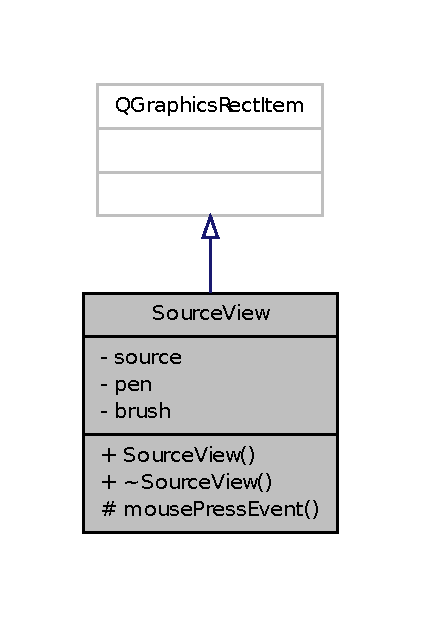
\includegraphics[width=202pt]{de/ddc/classSourceView__inherit__graph}
\end{center}
\end{figure}


Graphe de collaboration de Source\+View\+:\nopagebreak
\begin{figure}[H]
\begin{center}
\leavevmode
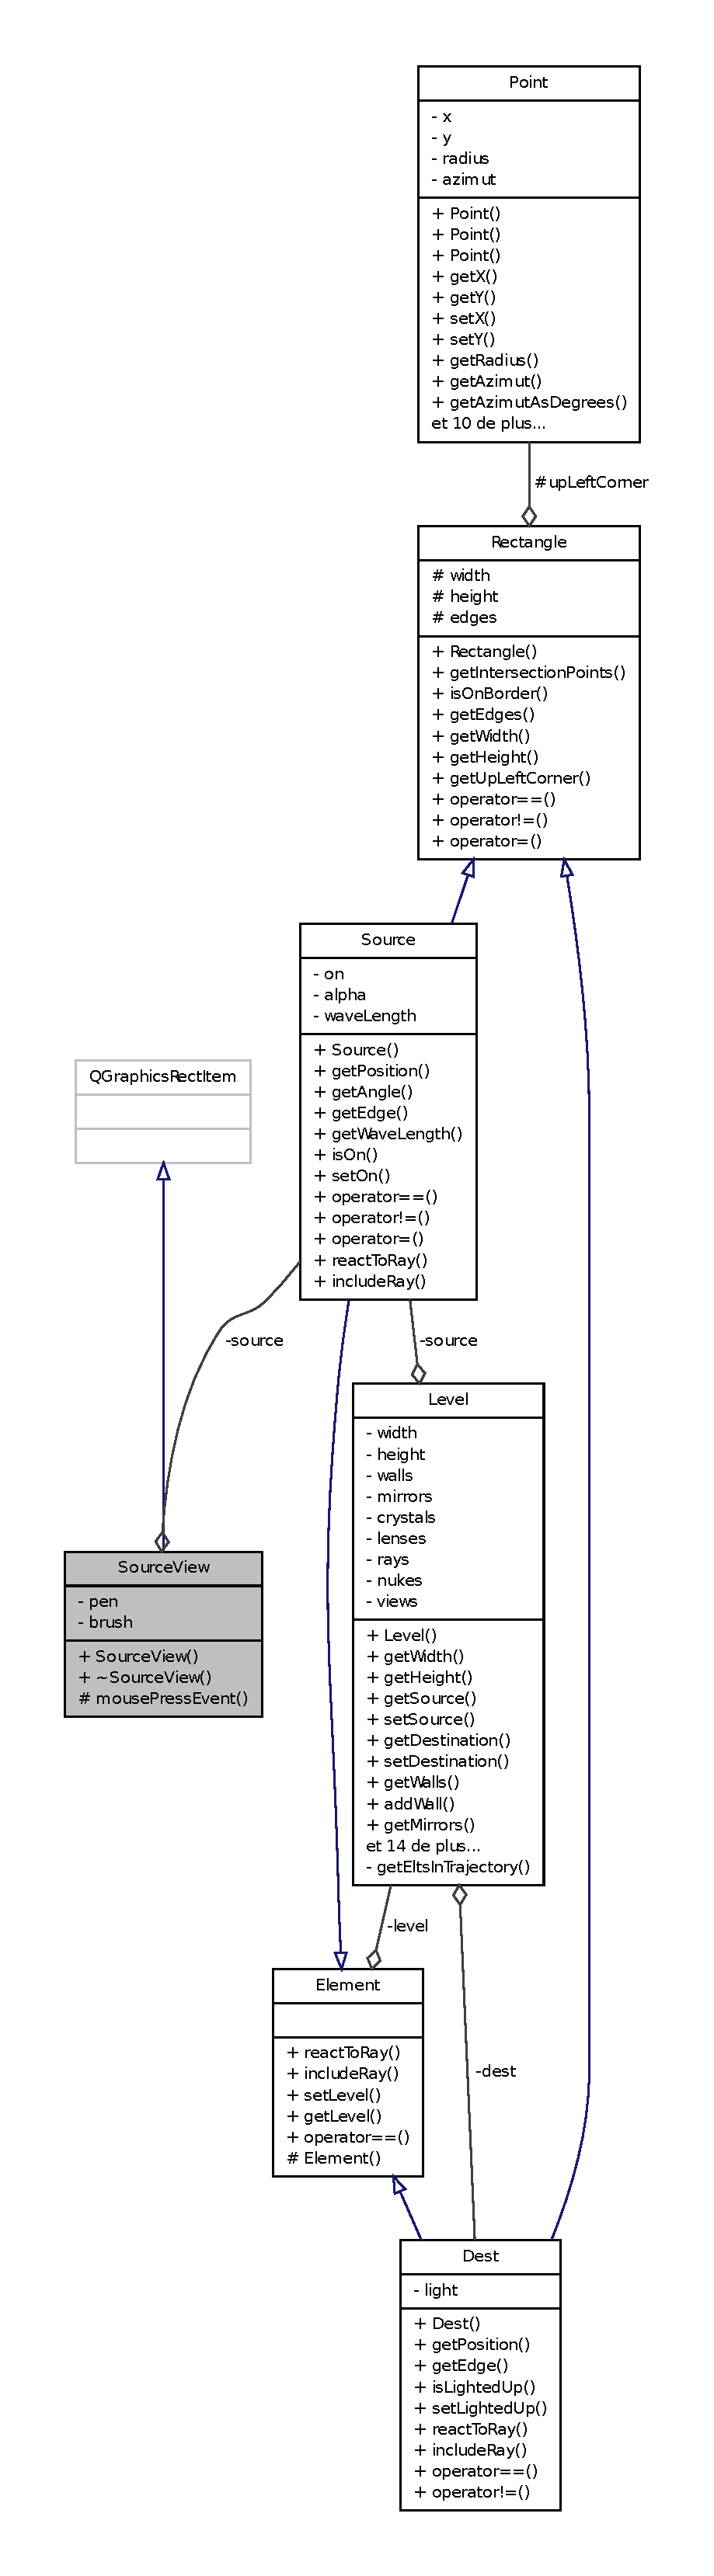
\includegraphics[height=550pt]{d2/df3/classSourceView__coll__graph}
\end{center}
\end{figure}


\subsection{Documentation des constructeurs et destructeur}
\hypertarget{classSourceView_a21ea9c4e88fc2cc79b9cd9001f7333f2}{}\index{Source\+View@{Source\+View}!Source\+View@{Source\+View}}
\index{Source\+View@{Source\+View}!Source\+View@{Source\+View}}
\subsubsection[{Source\+View(\+Source $\ast$)}]{\setlength{\rightskip}{0pt plus 5cm}Source\+View\+::\+Source\+View (
\begin{DoxyParamCaption}
\item[{{\bf Source} $\ast$}]{}
\end{DoxyParamCaption}
)}\label{classSourceView_a21ea9c4e88fc2cc79b9cd9001f7333f2}


Permet de créer une vue liée à une source. 


\begin{DoxyParams}{Paramètres}
{\em source} & La source liée à cette vue. \\
\hline
\end{DoxyParams}
\hypertarget{classSourceView_aee500dba1590df1506a972b245a65f37}{}\index{Source\+View@{Source\+View}!````~Source\+View@{$\sim$\+Source\+View}}
\index{````~Source\+View@{$\sim$\+Source\+View}!Source\+View@{Source\+View}}
\subsubsection[{$\sim$\+Source\+View()}]{\setlength{\rightskip}{0pt plus 5cm}Source\+View\+::$\sim$\+Source\+View (
\begin{DoxyParamCaption}
{}
\end{DoxyParamCaption}
)}\label{classSourceView_aee500dba1590df1506a972b245a65f37}


\subsection{Documentation des fonctions membres}
\hypertarget{classSourceView_af2fd6dc466853974e482701139ef66c9}{}\index{Source\+View@{Source\+View}!mouse\+Press\+Event@{mouse\+Press\+Event}}
\index{mouse\+Press\+Event@{mouse\+Press\+Event}!Source\+View@{Source\+View}}
\subsubsection[{mouse\+Press\+Event(\+Q\+Graphics\+Scene\+Mouse\+Event $\ast$)}]{\setlength{\rightskip}{0pt plus 5cm}void Source\+View\+::mouse\+Press\+Event (
\begin{DoxyParamCaption}
\item[{Q\+Graphics\+Scene\+Mouse\+Event $\ast$}]{}
\end{DoxyParamCaption}
)\hspace{0.3cm}{\ttfamily [protected]}}\label{classSourceView_af2fd6dc466853974e482701139ef66c9}


Permet de réagir sur le modèle lors d\textquotesingle{}un \char`\"{}input user\char`\"{}. 


\begin{DoxyParams}{Paramètres}
{\em event} & Un évènement \char`\"{}input user\char`\"{}. \\
\hline
\end{DoxyParams}


\subsection{Documentation des données membres}
\hypertarget{classSourceView_ab1337e79e435bc3310c34acef403d9d2}{}\index{Source\+View@{Source\+View}!brush@{brush}}
\index{brush@{brush}!Source\+View@{Source\+View}}
\subsubsection[{brush}]{\setlength{\rightskip}{0pt plus 5cm}Q\+Brush Source\+View\+::brush\hspace{0.3cm}{\ttfamily [private]}}\label{classSourceView_ab1337e79e435bc3310c34acef403d9d2}


Les paramètres visuels du plein de la source. 



Définition à la ligne 29 du fichier sourceview.\+hpp.

\hypertarget{classSourceView_a3f838e39f9e01a2a547b164c28193170}{}\index{Source\+View@{Source\+View}!pen@{pen}}
\index{pen@{pen}!Source\+View@{Source\+View}}
\subsubsection[{pen}]{\setlength{\rightskip}{0pt plus 5cm}Q\+Pen Source\+View\+::pen\hspace{0.3cm}{\ttfamily [private]}}\label{classSourceView_a3f838e39f9e01a2a547b164c28193170}


Les paramètres visuels du trait de la source. 



Définition à la ligne 24 du fichier sourceview.\+hpp.

\hypertarget{classSourceView_a79354c401511132bfe754ce5d92b8d23}{}\index{Source\+View@{Source\+View}!source@{source}}
\index{source@{source}!Source\+View@{Source\+View}}
\subsubsection[{source}]{\setlength{\rightskip}{0pt plus 5cm}{\bf Source}$\ast$ Source\+View\+::source\hspace{0.3cm}{\ttfamily [private]}}\label{classSourceView_a79354c401511132bfe754ce5d92b8d23}


La source représentée par cette vue. 



Définition à la ligne 19 du fichier sourceview.\+hpp.



La documentation de cette classe a été générée à partir du fichier suivant \+:\begin{DoxyCompactItemize}
\item 
view/dynamic\+Elements/\hyperlink{sourceview_8hpp}{sourceview.\+hpp}\end{DoxyCompactItemize}

\hypertarget{classStarlightException}{}\section{Référence de la classe Starlight\+Exception}
\label{classStarlightException}\index{Starlight\+Exception@{Starlight\+Exception}}


Cette classe représente une exception spécifique au jeu Starlight.  




{\ttfamily \#include $<$starlightexception.\+hpp$>$}

\subsection*{Fonctions membres publiques}
\begin{DoxyCompactItemize}
\item 
\hyperlink{classStarlightException_a36d43a3c21c61b15a8dc4b3e15f12ab0}{Starlight\+Exception} (std\+::string)
\begin{DoxyCompactList}\small\item\em Construit une nouvelle erreur inhérente au jeu. \end{DoxyCompactList}\item 
std\+::string \hyperlink{classStarlightException_ae4c499f366c74c29dc36c935aa665dda}{get\+Message} () const 
\begin{DoxyCompactList}\small\item\em Permet d\textquotesingle{}obtenir le message d\textquotesingle{}erreur de l\textquotesingle{}exception. \end{DoxyCompactList}\item 
const char $\ast$ \hyperlink{classStarlightException_a727446aaf06aa9bc92d63ff21a37049b}{what} () const   throw ()
\begin{DoxyCompactList}\small\item\em Permet d\textquotesingle{}afficher l\textquotesingle{}erreur en cas d\textquotesingle{}erreur. \end{DoxyCompactList}\end{DoxyCompactItemize}
\subsection*{Attributs privés}
\begin{DoxyCompactItemize}
\item 
std\+::string \hyperlink{classStarlightException_aa235f0c10c5ad918b0c2911c72a85fcb}{error\+Msg}
\begin{DoxyCompactList}\small\item\em Le message d\textquotesingle{}erreur de l\textquotesingle{}exception lancée. \end{DoxyCompactList}\end{DoxyCompactItemize}


\subsection{Description détaillée}
Cette classe représente une exception spécifique au jeu Starlight. 

Définition à la ligne 10 du fichier starlightexception.\+hpp.



Graphe d\textquotesingle{}héritage de Starlight\+Exception\+:\nopagebreak
\begin{figure}[H]
\begin{center}
\leavevmode
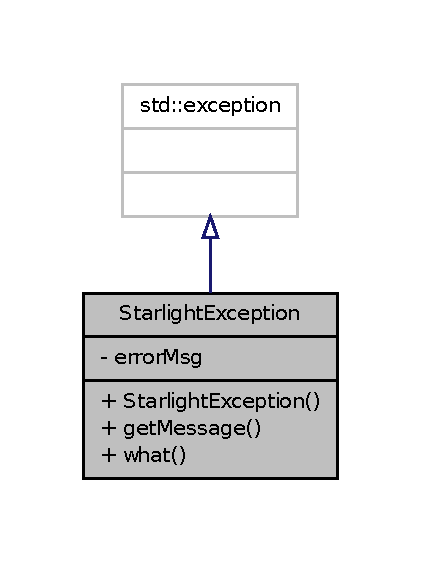
\includegraphics[width=202pt]{da/dcd/classStarlightException__inherit__graph}
\end{center}
\end{figure}


Graphe de collaboration de Starlight\+Exception\+:\nopagebreak
\begin{figure}[H]
\begin{center}
\leavevmode
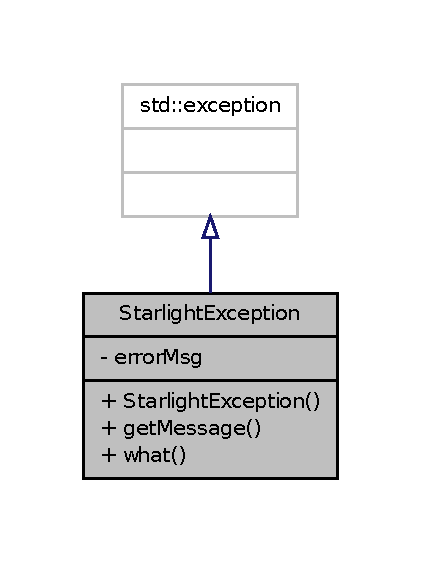
\includegraphics[width=202pt]{dd/d88/classStarlightException__coll__graph}
\end{center}
\end{figure}


\subsection{Documentation des constructeurs et destructeur}
\hypertarget{classStarlightException_a36d43a3c21c61b15a8dc4b3e15f12ab0}{}\index{Starlight\+Exception@{Starlight\+Exception}!Starlight\+Exception@{Starlight\+Exception}}
\index{Starlight\+Exception@{Starlight\+Exception}!Starlight\+Exception@{Starlight\+Exception}}
\subsubsection[{Starlight\+Exception(std\+::string)}]{\setlength{\rightskip}{0pt plus 5cm}Starlight\+Exception\+::\+Starlight\+Exception (
\begin{DoxyParamCaption}
\item[{std\+::string}]{}
\end{DoxyParamCaption}
)}\label{classStarlightException_a36d43a3c21c61b15a8dc4b3e15f12ab0}


Construit une nouvelle erreur inhérente au jeu. 


\begin{DoxyParams}{Paramètres}
{\em error\+Msg} & Message expliquant l\textquotesingle{}erreur. \\
\hline
\end{DoxyParams}


\subsection{Documentation des fonctions membres}
\hypertarget{classStarlightException_ae4c499f366c74c29dc36c935aa665dda}{}\index{Starlight\+Exception@{Starlight\+Exception}!get\+Message@{get\+Message}}
\index{get\+Message@{get\+Message}!Starlight\+Exception@{Starlight\+Exception}}
\subsubsection[{get\+Message() const }]{\setlength{\rightskip}{0pt plus 5cm}std\+::string Starlight\+Exception\+::get\+Message (
\begin{DoxyParamCaption}
{}
\end{DoxyParamCaption}
) const\hspace{0.3cm}{\ttfamily [inline]}}\label{classStarlightException_ae4c499f366c74c29dc36c935aa665dda}


Permet d\textquotesingle{}obtenir le message d\textquotesingle{}erreur de l\textquotesingle{}exception. 

\begin{DoxyReturn}{Renvoie}
Le message d\textquotesingle{}erreur de l\textquotesingle{}exception. 
\end{DoxyReturn}


Définition à la ligne 45 du fichier starlightexception.\+hpp.



Références error\+Msg.


\begin{DoxyCode}
46 \{
47     \textcolor{keywordflow}{return} this->\hyperlink{classStarlightException_aa235f0c10c5ad918b0c2911c72a85fcb}{errorMsg};
48 \}
\end{DoxyCode}
\hypertarget{classStarlightException_a727446aaf06aa9bc92d63ff21a37049b}{}\index{Starlight\+Exception@{Starlight\+Exception}!what@{what}}
\index{what@{what}!Starlight\+Exception@{Starlight\+Exception}}
\subsubsection[{what() const }]{\setlength{\rightskip}{0pt plus 5cm}const char $\ast$ Starlight\+Exception\+::what (
\begin{DoxyParamCaption}
{}
\end{DoxyParamCaption}
) const throw  ) \hspace{0.3cm}{\ttfamily [inline]}}\label{classStarlightException_a727446aaf06aa9bc92d63ff21a37049b}


Permet d\textquotesingle{}afficher l\textquotesingle{}erreur en cas d\textquotesingle{}erreur. 

\begin{DoxyReturn}{Renvoie}
Le message d\textquotesingle{}erreur. 
\end{DoxyReturn}


Définition à la ligne 50 du fichier starlightexception.\+hpp.


\begin{DoxyCode}
51 \{
52     \textcolor{keywordflow}{return} this->\hyperlink{classStarlightException_aa235f0c10c5ad918b0c2911c72a85fcb}{errorMsg}.c\_str();
53 \}
\end{DoxyCode}


\subsection{Documentation des données membres}
\hypertarget{classStarlightException_aa235f0c10c5ad918b0c2911c72a85fcb}{}\index{Starlight\+Exception@{Starlight\+Exception}!error\+Msg@{error\+Msg}}
\index{error\+Msg@{error\+Msg}!Starlight\+Exception@{Starlight\+Exception}}
\subsubsection[{error\+Msg}]{\setlength{\rightskip}{0pt plus 5cm}std\+::string Starlight\+Exception\+::error\+Msg\hspace{0.3cm}{\ttfamily [private]}}\label{classStarlightException_aa235f0c10c5ad918b0c2911c72a85fcb}


Le message d\textquotesingle{}erreur de l\textquotesingle{}exception lancée. 



Définition à la ligne 18 du fichier starlightexception.\+hpp.



Référencé par get\+Message().



La documentation de cette classe a été générée à partir du fichier suivant \+:\begin{DoxyCompactItemize}
\item 
model/exception/\hyperlink{starlightexception_8hpp}{starlightexception.\+hpp}\end{DoxyCompactItemize}

\hypertarget{classWall}{}\section{Référence de la classe Wall}
\label{classWall}\index{Wall@{Wall}}


Cette classe modélise les murs utilisés dans le jeu.  




{\ttfamily \#include $<$wall.\+hpp$>$}

\subsection*{Fonctions membres publiques}
\begin{DoxyCompactItemize}
\item 
\hyperlink{classWall_aa9e4665888cfb76c5700fcd9f8672771}{Wall} (const \hyperlink{classPoint}{Point} \&, const \hyperlink{classPoint}{Point} \&)
\begin{DoxyCompactList}\small\item\em Instancie un mur. \end{DoxyCompactList}\item 
const \hyperlink{classPoint}{Point} \& \hyperlink{classWall_af21a88dc50de229830bbfe68f088e5f2}{get\+Start} () const 
\begin{DoxyCompactList}\small\item\em Retourne le début du mur. \end{DoxyCompactList}\item 
const \hyperlink{classPoint}{Point} \& \hyperlink{classWall_aeae40b7ecf22bd44dc75382bafad24c8}{get\+End} () const 
\begin{DoxyCompactList}\small\item\em Retourne la fin du mur. \end{DoxyCompactList}\item 
void \hyperlink{classWall_a4167a9d310ff17cf02d232d4f384b77d}{react\+To\+Ray} (\hyperlink{classRay}{Ray})
\begin{DoxyCompactList}\small\item\em Réaction à l\textquotesingle{}exposition d\textquotesingle{}un rayon. \end{DoxyCompactList}\item 
\hyperlink{classPoint}{Point} $\ast$ \hyperlink{classWall_a11178e8dc8eabc9a56b9bf5525dc4f29}{include\+Ray} (const \hyperlink{classRay}{Ray} \&) const 
\begin{DoxyCompactList}\small\item\em Renseigne si le mur est dans la trajectoire du rayon. \end{DoxyCompactList}\item 
bool \hyperlink{classWall_a56676feaace7ad556d8c94a195afb5da}{operator==} (const \hyperlink{classWall}{Wall} \&) const 
\begin{DoxyCompactList}\small\item\em Permet de savoir si deux murs sont identiques. \end{DoxyCompactList}\item 
bool \hyperlink{classWall_a2a918fa1c882900fe5cf97cf8d9da130}{operator!=} (const \hyperlink{classWall}{Wall} \&) const 
\begin{DoxyCompactList}\small\item\em Permet de savoir si deux murs sont différents. \end{DoxyCompactList}\end{DoxyCompactItemize}
\subsection*{Attributs privés}
\begin{DoxyCompactItemize}
\item 
\hyperlink{classPoint}{Point} \hyperlink{classWall_a05a052498fc50c585a8e8be95dc5af01}{start}
\begin{DoxyCompactList}\small\item\em Le point de départ du segment de droite représentant le mur. \end{DoxyCompactList}\item 
\hyperlink{classPoint}{Point} \hyperlink{classWall_a26e8075259c6cd51630b546f3e37d2a1}{end}
\begin{DoxyCompactList}\small\item\em Le point d\textquotesingle{}arrivé du segment de droite représentant le mur. \end{DoxyCompactList}\end{DoxyCompactItemize}
\subsection*{Membres hérités additionnels}


\subsection{Description détaillée}
Cette classe modélise les murs utilisés dans le jeu. 

Les murs sont des segments de droite qui ne réfléchissent pas la lumière. 

Définition à la ligne 16 du fichier wall.\+hpp.



Graphe d\textquotesingle{}héritage de Wall\+:\nopagebreak
\begin{figure}[H]
\begin{center}
\leavevmode
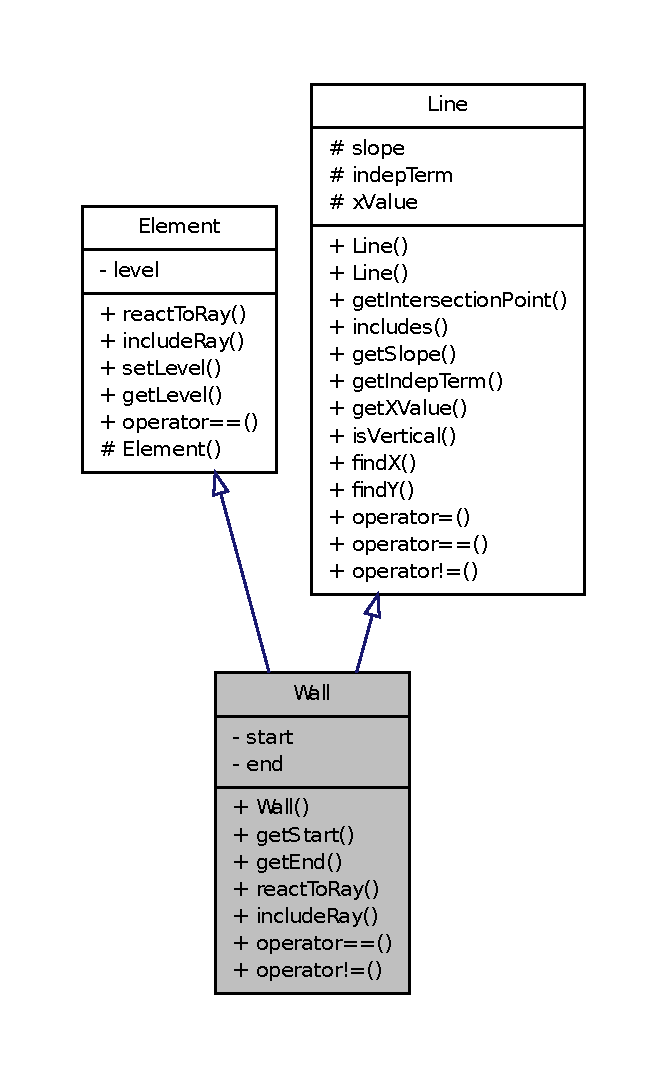
\includegraphics[width=320pt]{de/d28/classWall__inherit__graph}
\end{center}
\end{figure}


Graphe de collaboration de Wall\+:\nopagebreak
\begin{figure}[H]
\begin{center}
\leavevmode
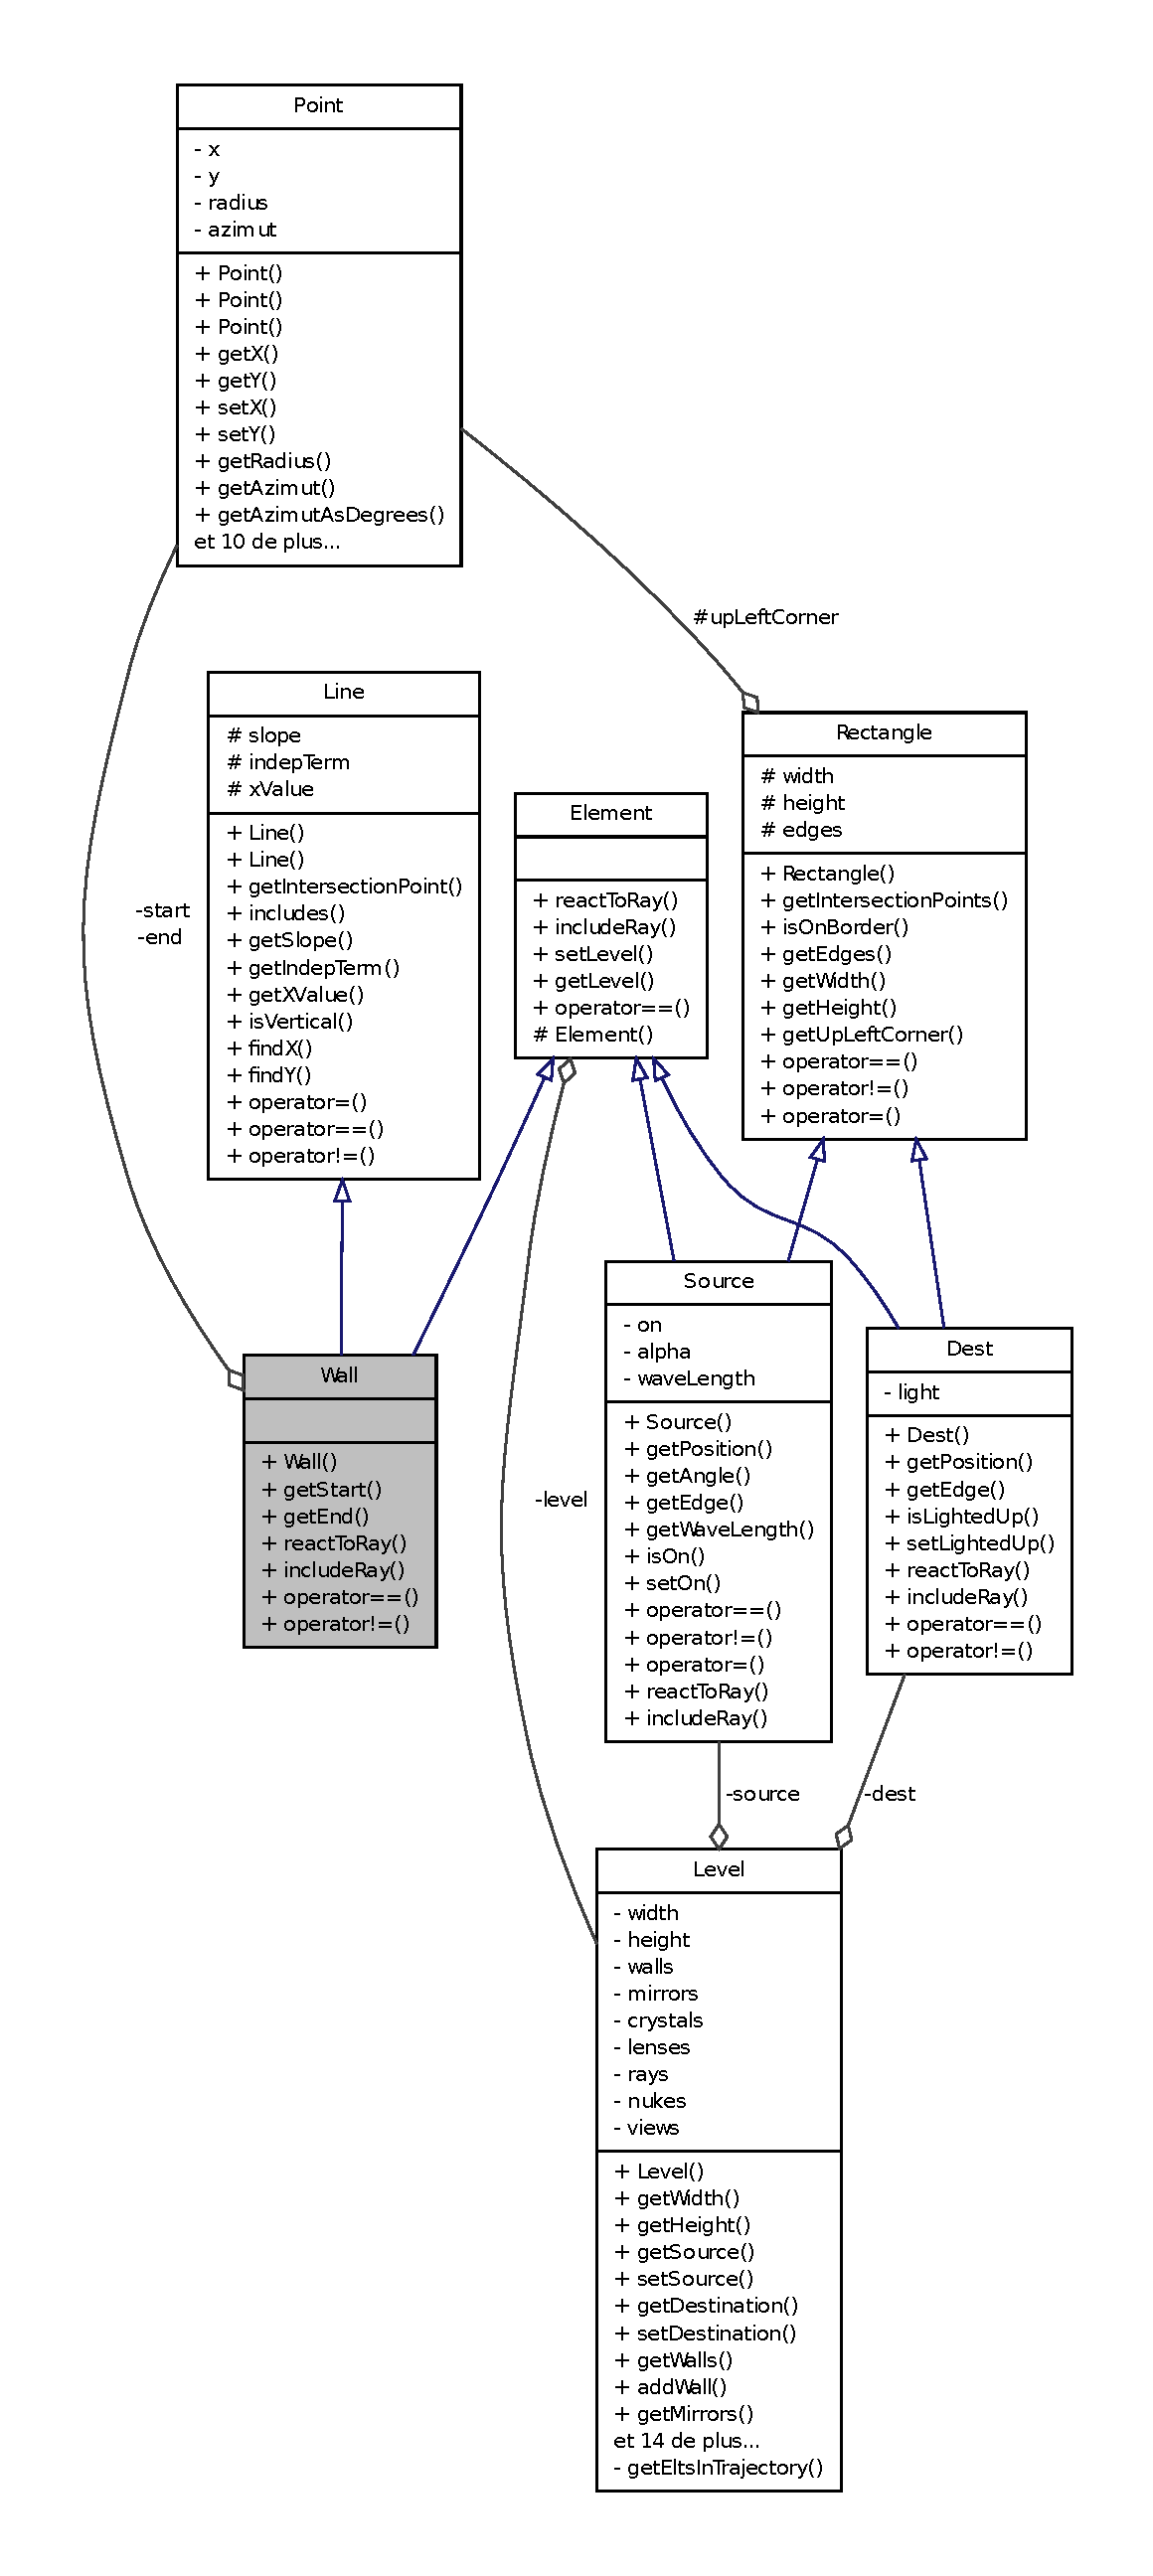
\includegraphics[height=550pt]{d9/d82/classWall__coll__graph}
\end{center}
\end{figure}


\subsection{Documentation des constructeurs et destructeur}
\hypertarget{classWall_aa9e4665888cfb76c5700fcd9f8672771}{}\index{Wall@{Wall}!Wall@{Wall}}
\index{Wall@{Wall}!Wall@{Wall}}
\subsubsection[{Wall(const Point \&, const Point \&)}]{\setlength{\rightskip}{0pt plus 5cm}Wall\+::\+Wall (
\begin{DoxyParamCaption}
\item[{const {\bf Point} \&}]{, }
\item[{const {\bf Point} \&}]{}
\end{DoxyParamCaption}
)}\label{classWall_aa9e4665888cfb76c5700fcd9f8672771}


Instancie un mur. 


\begin{DoxyParams}{Paramètres}
{\em start} & Le début du mur. \\
\hline
{\em end} & La fin du mur. \\
\hline
\end{DoxyParams}


\subsection{Documentation des fonctions membres}
\hypertarget{classWall_aeae40b7ecf22bd44dc75382bafad24c8}{}\index{Wall@{Wall}!get\+End@{get\+End}}
\index{get\+End@{get\+End}!Wall@{Wall}}
\subsubsection[{get\+End() const }]{\setlength{\rightskip}{0pt plus 5cm}const {\bf Point} \& Wall\+::get\+End (
\begin{DoxyParamCaption}
{}
\end{DoxyParamCaption}
) const\hspace{0.3cm}{\ttfamily [inline]}}\label{classWall_aeae40b7ecf22bd44dc75382bafad24c8}


Retourne la fin du mur. 

\begin{DoxyReturn}{Renvoie}
La fin du mur. 
\end{DoxyReturn}


Définition à la ligne 97 du fichier wall.\+hpp.



Références end.


\begin{DoxyCode}
98 \{
99     \textcolor{keywordflow}{return} this->\hyperlink{classWall_a26e8075259c6cd51630b546f3e37d2a1}{end};
100 \}
\end{DoxyCode}
\hypertarget{classWall_af21a88dc50de229830bbfe68f088e5f2}{}\index{Wall@{Wall}!get\+Start@{get\+Start}}
\index{get\+Start@{get\+Start}!Wall@{Wall}}
\subsubsection[{get\+Start() const }]{\setlength{\rightskip}{0pt plus 5cm}const {\bf Point} \& Wall\+::get\+Start (
\begin{DoxyParamCaption}
{}
\end{DoxyParamCaption}
) const\hspace{0.3cm}{\ttfamily [inline]}}\label{classWall_af21a88dc50de229830bbfe68f088e5f2}


Retourne le début du mur. 

\begin{DoxyReturn}{Renvoie}
Le début du mur. 
\end{DoxyReturn}


Définition à la ligne 92 du fichier wall.\+hpp.



Références start.


\begin{DoxyCode}
93 \{
94     \textcolor{keywordflow}{return} this->\hyperlink{classWall_a05a052498fc50c585a8e8be95dc5af01}{start};
95 \}
\end{DoxyCode}
\hypertarget{classWall_a11178e8dc8eabc9a56b9bf5525dc4f29}{}\index{Wall@{Wall}!include\+Ray@{include\+Ray}}
\index{include\+Ray@{include\+Ray}!Wall@{Wall}}
\subsubsection[{include\+Ray(const Ray \&) const }]{\setlength{\rightskip}{0pt plus 5cm}{\bf Point}$\ast$ Wall\+::include\+Ray (
\begin{DoxyParamCaption}
\item[{const {\bf Ray} \&}]{}
\end{DoxyParamCaption}
) const\hspace{0.3cm}{\ttfamily [virtual]}}\label{classWall_a11178e8dc8eabc9a56b9bf5525dc4f29}


Renseigne si le mur est dans la trajectoire du rayon. 


\begin{DoxyParams}{Paramètres}
{\em ray} & Le rayon.\\
\hline
\end{DoxyParams}
\begin{DoxyReturn}{Renvoie}
{\ttfamily true} Si la mur se trouve dans la trajectoire du rayon entré en paramètre. 
\end{DoxyReturn}


Implémente \hyperlink{classElement_a1b88519623a6250155f7182706665448}{Element}.

\hypertarget{classWall_a2a918fa1c882900fe5cf97cf8d9da130}{}\index{Wall@{Wall}!operator"!=@{operator"!=}}
\index{operator"!=@{operator"!=}!Wall@{Wall}}
\subsubsection[{operator"!=(const Wall \&) const }]{\setlength{\rightskip}{0pt plus 5cm}bool Wall\+::operator!= (
\begin{DoxyParamCaption}
\item[{const {\bf Wall} \&}]{}
\end{DoxyParamCaption}
) const}\label{classWall_a2a918fa1c882900fe5cf97cf8d9da130}


Permet de savoir si deux murs sont différents. 

\begin{DoxyReturn}{Renvoie}
{\ttfamily true} Si les murs sont différents. 
\end{DoxyReturn}
\hypertarget{classWall_a56676feaace7ad556d8c94a195afb5da}{}\index{Wall@{Wall}!operator==@{operator==}}
\index{operator==@{operator==}!Wall@{Wall}}
\subsubsection[{operator==(const Wall \&) const }]{\setlength{\rightskip}{0pt plus 5cm}bool Wall\+::operator== (
\begin{DoxyParamCaption}
\item[{const {\bf Wall} \&}]{}
\end{DoxyParamCaption}
) const}\label{classWall_a56676feaace7ad556d8c94a195afb5da}


Permet de savoir si deux murs sont identiques. 

\begin{DoxyReturn}{Renvoie}
{\ttfamily true} Si les murs sont les même. 
\end{DoxyReturn}
\hypertarget{classWall_a4167a9d310ff17cf02d232d4f384b77d}{}\index{Wall@{Wall}!react\+To\+Ray@{react\+To\+Ray}}
\index{react\+To\+Ray@{react\+To\+Ray}!Wall@{Wall}}
\subsubsection[{react\+To\+Ray(\+Ray)}]{\setlength{\rightskip}{0pt plus 5cm}void Wall\+::react\+To\+Ray (
\begin{DoxyParamCaption}
\item[{{\bf Ray}}]{}
\end{DoxyParamCaption}
)\hspace{0.3cm}{\ttfamily [virtual]}}\label{classWall_a4167a9d310ff17cf02d232d4f384b77d}


Réaction à l\textquotesingle{}exposition d\textquotesingle{}un rayon. 


\begin{DoxyParams}{Paramètres}
{\em ray} & Le rayon. \\
\hline
\end{DoxyParams}


Implémente \hyperlink{classElement_aa87116bb9422d64169b2ebf03831df9b}{Element}.



\subsection{Documentation des données membres}
\hypertarget{classWall_a26e8075259c6cd51630b546f3e37d2a1}{}\index{Wall@{Wall}!end@{end}}
\index{end@{end}!Wall@{Wall}}
\subsubsection[{end}]{\setlength{\rightskip}{0pt plus 5cm}{\bf Point} Wall\+::end\hspace{0.3cm}{\ttfamily [private]}}\label{classWall_a26e8075259c6cd51630b546f3e37d2a1}


Le point d\textquotesingle{}arrivé du segment de droite représentant le mur. 



Définition à la ligne 26 du fichier wall.\+hpp.



Référencé par get\+End().

\hypertarget{classWall_a05a052498fc50c585a8e8be95dc5af01}{}\index{Wall@{Wall}!start@{start}}
\index{start@{start}!Wall@{Wall}}
\subsubsection[{start}]{\setlength{\rightskip}{0pt plus 5cm}{\bf Point} Wall\+::start\hspace{0.3cm}{\ttfamily [private]}}\label{classWall_a05a052498fc50c585a8e8be95dc5af01}


Le point de départ du segment de droite représentant le mur. 



Définition à la ligne 21 du fichier wall.\+hpp.



Référencé par get\+Start().



La documentation de cette classe a été générée à partir du fichier suivant \+:\begin{DoxyCompactItemize}
\item 
model/elements/\hyperlink{wall_8hpp}{wall.\+hpp}\end{DoxyCompactItemize}

\chapter{Documentation des fichiers}
\hypertarget{main_8cpp}{}\section{Référence du fichier main.\+cpp}
\label{main_8cpp}\index{main.\+cpp@{main.\+cpp}}
{\ttfamily \#include \char`\"{}main.\+hpp\char`\"{}}\\*
{\ttfamily \#include $<$Q\+Application$>$}\\*
{\ttfamily \#include \char`\"{}view/windows/mainwindow.\+hpp\char`\"{}}\\*
Graphe des dépendances par inclusion de main.\+cpp\+:\nopagebreak
\begin{figure}[H]
\begin{center}
\leavevmode
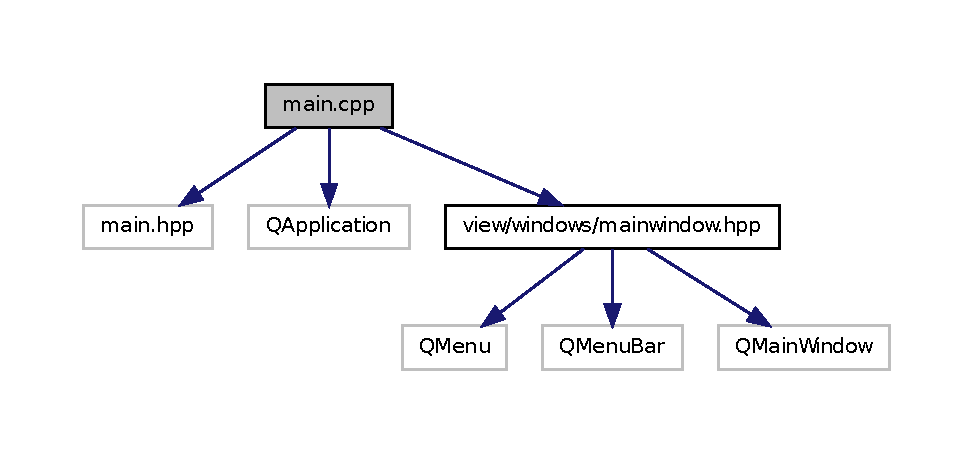
\includegraphics[width=350pt]{da/dce/main_8cpp__incl}
\end{center}
\end{figure}
\subsection*{Fonctions}
\begin{DoxyCompactItemize}
\item 
int \hyperlink{main_8cpp_a0ddf1224851353fc92bfbff6f499fa97}{main} (int argc, char $\ast$argv\mbox{[}$\,$\mbox{]})
\end{DoxyCompactItemize}


\subsection{Documentation des fonctions}
\hypertarget{main_8cpp_a0ddf1224851353fc92bfbff6f499fa97}{}\index{main.\+cpp@{main.\+cpp}!main@{main}}
\index{main@{main}!main.\+cpp@{main.\+cpp}}
\subsubsection[{main(int argc, char $\ast$argv[])}]{\setlength{\rightskip}{0pt plus 5cm}int main (
\begin{DoxyParamCaption}
\item[{int}]{argc, }
\item[{char $\ast$}]{argv\mbox{[}$\,$\mbox{]}}
\end{DoxyParamCaption}
)}\label{main_8cpp_a0ddf1224851353fc92bfbff6f499fa97}


Définition à la ligne 8 du fichier main.\+cpp.


\begin{DoxyCode}
9 \{
10     QApplication a(argc, argv);
11     \hyperlink{classMainWindow}{MainWindow} w;
12 
13     w.show();
14 
15     \textcolor{keywordflow}{return} a.exec();
16 \}
\end{DoxyCode}

\hypertarget{crystal_8hpp}{}\section{Référence du fichier model/elements/crystal.hpp}
\label{crystal_8hpp}\index{model/elements/crystal.\+hpp@{model/elements/crystal.\+hpp}}
{\ttfamily \#include $<$ostream$>$}\\*
{\ttfamily \#include \char`\"{}model/elements/element.\+hpp\char`\"{}}\\*
{\ttfamily \#include \char`\"{}model/geometry/ellipse.\+hpp\char`\"{}}\\*
{\ttfamily \#include \char`\"{}model/geometry/utilities.\+hpp\char`\"{}}\\*
Graphe des dépendances par inclusion de crystal.\+hpp\+:\nopagebreak
\begin{figure}[H]
\begin{center}
\leavevmode
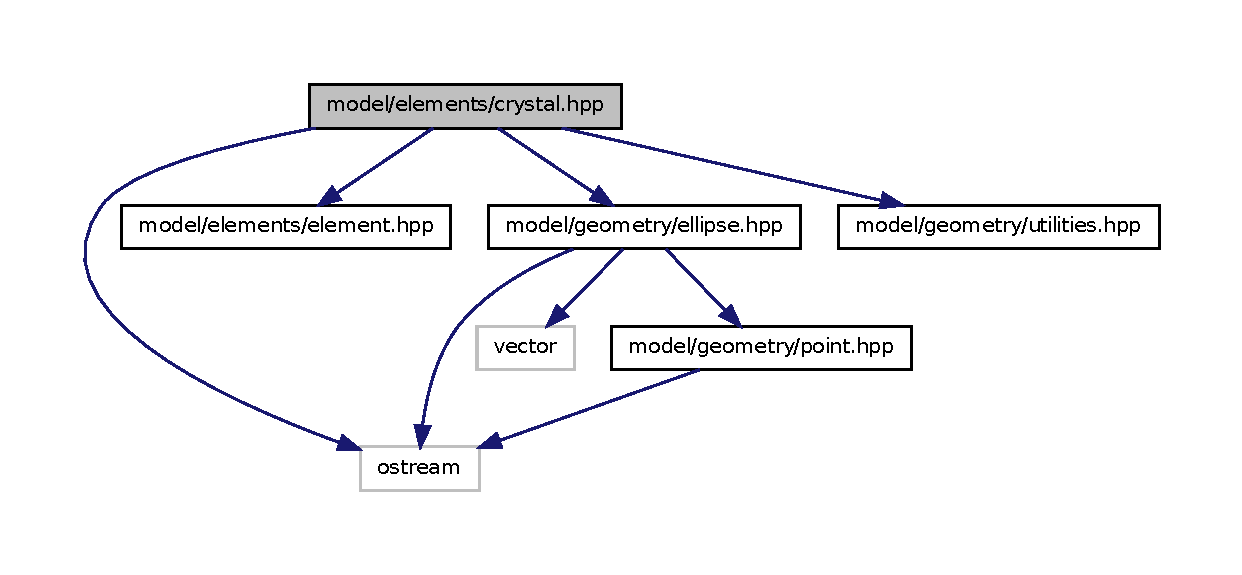
\includegraphics[width=350pt]{da/d84/crystal_8hpp__incl}
\end{center}
\end{figure}
Ce graphe montre quels fichiers incluent directement ou indirectement ce fichier \+:\nopagebreak
\begin{figure}[H]
\begin{center}
\leavevmode
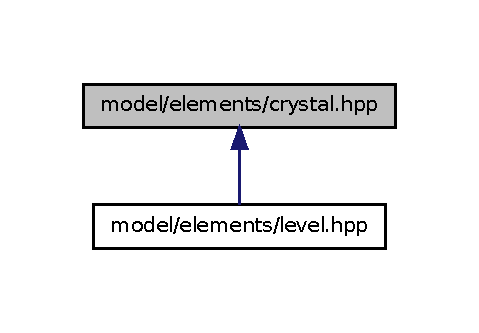
\includegraphics[width=230pt]{d4/d95/crystal_8hpp__dep__incl}
\end{center}
\end{figure}
\subsection*{Classes}
\begin{DoxyCompactItemize}
\item 
class \hyperlink{classCrystal}{Crystal}
\begin{DoxyCompactList}\small\item\em Cette classe amplifie les cristaux utilisés dans le jeu. \end{DoxyCompactList}\end{DoxyCompactItemize}
\subsection*{Fonctions}
\begin{DoxyCompactItemize}
\item 
std\+::ostream \& \hyperlink{crystal_8hpp_a45da91e3993e90a57a5f4fd5edda0adb}{operator$<$$<$} (std\+::ostream \&, const \hyperlink{classCrystal}{Crystal} \&)
\begin{DoxyCompactList}\small\item\em Définition, externe, de l\textquotesingle{}opérateur permettant de produire un affichage formaté. \end{DoxyCompactList}\end{DoxyCompactItemize}


\subsection{Documentation des fonctions}
\hypertarget{crystal_8hpp_a45da91e3993e90a57a5f4fd5edda0adb}{}\index{crystal.\+hpp@{crystal.\+hpp}!operator$<$$<$@{operator$<$$<$}}
\index{operator$<$$<$@{operator$<$$<$}!crystal.\+hpp@{crystal.\+hpp}}
\subsubsection[{operator$<$$<$(std\+::ostream \&, const Crystal \&)}]{\setlength{\rightskip}{0pt plus 5cm}std\+::ostream\& operator$<$$<$ (
\begin{DoxyParamCaption}
\item[{std\+::ostream \&}]{, }
\item[{const {\bf Crystal} \&}]{}
\end{DoxyParamCaption}
)}\label{crystal_8hpp_a45da91e3993e90a57a5f4fd5edda0adb}


Définition, externe, de l\textquotesingle{}opérateur permettant de produire un affichage formaté. 

\begin{DoxyReturn}{Renvoie}
Le ostream rempli de la chaine formatée représentant le \hyperlink{classCrystal}{Crystal} en paramètre. 
\end{DoxyReturn}

\hypertarget{dest_8hpp}{}\section{Référence du fichier model/elements/dest.hpp}
\label{dest_8hpp}\index{model/elements/dest.\+hpp@{model/elements/dest.\+hpp}}
{\ttfamily \#include $<$ostream$>$}\\*
{\ttfamily \#include \char`\"{}model/elements/element.\+hpp\char`\"{}}\\*
{\ttfamily \#include \char`\"{}model/geometry/rectangle.\+hpp\char`\"{}}\\*
Graphe des dépendances par inclusion de dest.\+hpp\+:\nopagebreak
\begin{figure}[H]
\begin{center}
\leavevmode
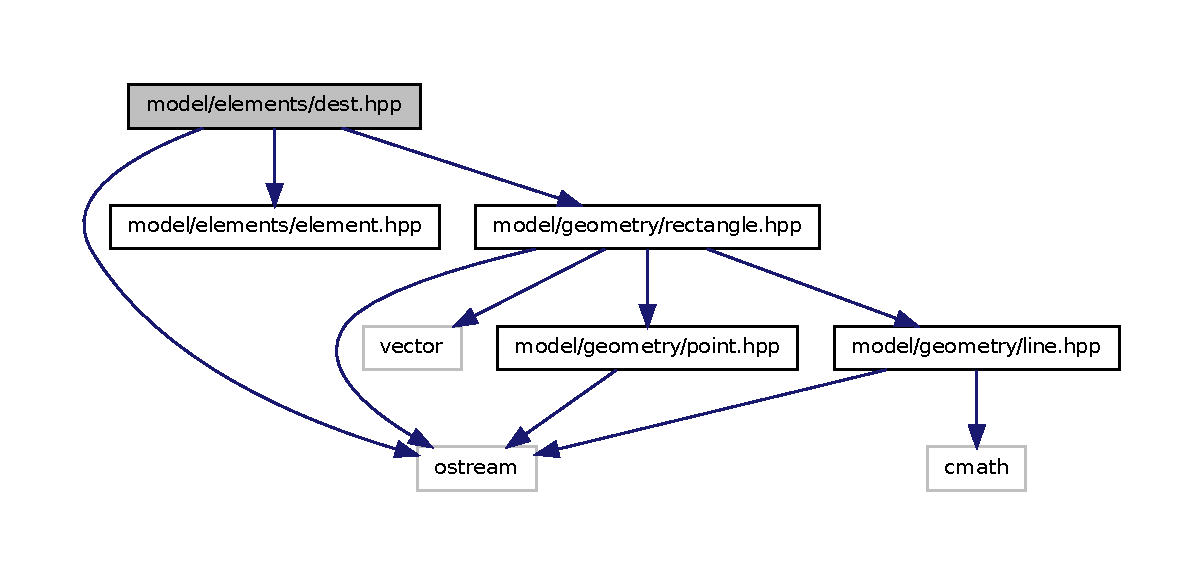
\includegraphics[width=350pt]{db/d67/dest_8hpp__incl}
\end{center}
\end{figure}
Ce graphe montre quels fichiers incluent directement ou indirectement ce fichier \+:\nopagebreak
\begin{figure}[H]
\begin{center}
\leavevmode
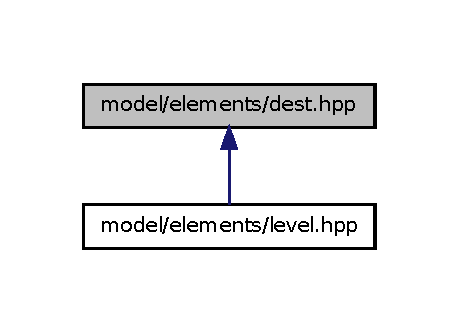
\includegraphics[width=220pt]{de/d6c/dest_8hpp__dep__incl}
\end{center}
\end{figure}
\subsection*{Classes}
\begin{DoxyCompactItemize}
\item 
class \hyperlink{classDest}{Dest}
\begin{DoxyCompactList}\small\item\em Cette classe modélise la destination utilisée dans le jeu. \end{DoxyCompactList}\end{DoxyCompactItemize}
\subsection*{Fonctions}
\begin{DoxyCompactItemize}
\item 
std\+::ostream \& \hyperlink{dest_8hpp_ae50140bc92da1c3f8baf098292e086ef}{operator$<$$<$} (std\+::ostream \&, const \hyperlink{classDest}{Dest} \&)
\begin{DoxyCompactList}\small\item\em Définition, externe, de l\textquotesingle{}opérateur permettant de produire un affichage formaté. \end{DoxyCompactList}\end{DoxyCompactItemize}


\subsection{Documentation des fonctions}
\hypertarget{dest_8hpp_ae50140bc92da1c3f8baf098292e086ef}{}\index{dest.\+hpp@{dest.\+hpp}!operator$<$$<$@{operator$<$$<$}}
\index{operator$<$$<$@{operator$<$$<$}!dest.\+hpp@{dest.\+hpp}}
\subsubsection[{operator$<$$<$(std\+::ostream \&, const Dest \&)}]{\setlength{\rightskip}{0pt plus 5cm}std\+::ostream\& operator$<$$<$ (
\begin{DoxyParamCaption}
\item[{std\+::ostream \&}]{, }
\item[{const {\bf Dest} \&}]{}
\end{DoxyParamCaption}
)}\label{dest_8hpp_ae50140bc92da1c3f8baf098292e086ef}


Définition, externe, de l\textquotesingle{}opérateur permettant de produire un affichage formaté. 

\begin{DoxyReturn}{Renvoie}
Le ostream rempli de la chaine formatée représentant la \hyperlink{classDest}{Dest} en paramètre. 
\end{DoxyReturn}

\hypertarget{element_8hpp}{}\section{Référence du fichier model/elements/element.hpp}
\label{element_8hpp}\index{model/elements/element.\+hpp@{model/elements/element.\+hpp}}
Ce graphe montre quels fichiers incluent directement ou indirectement ce fichier \+:\nopagebreak
\begin{figure}[H]
\begin{center}
\leavevmode
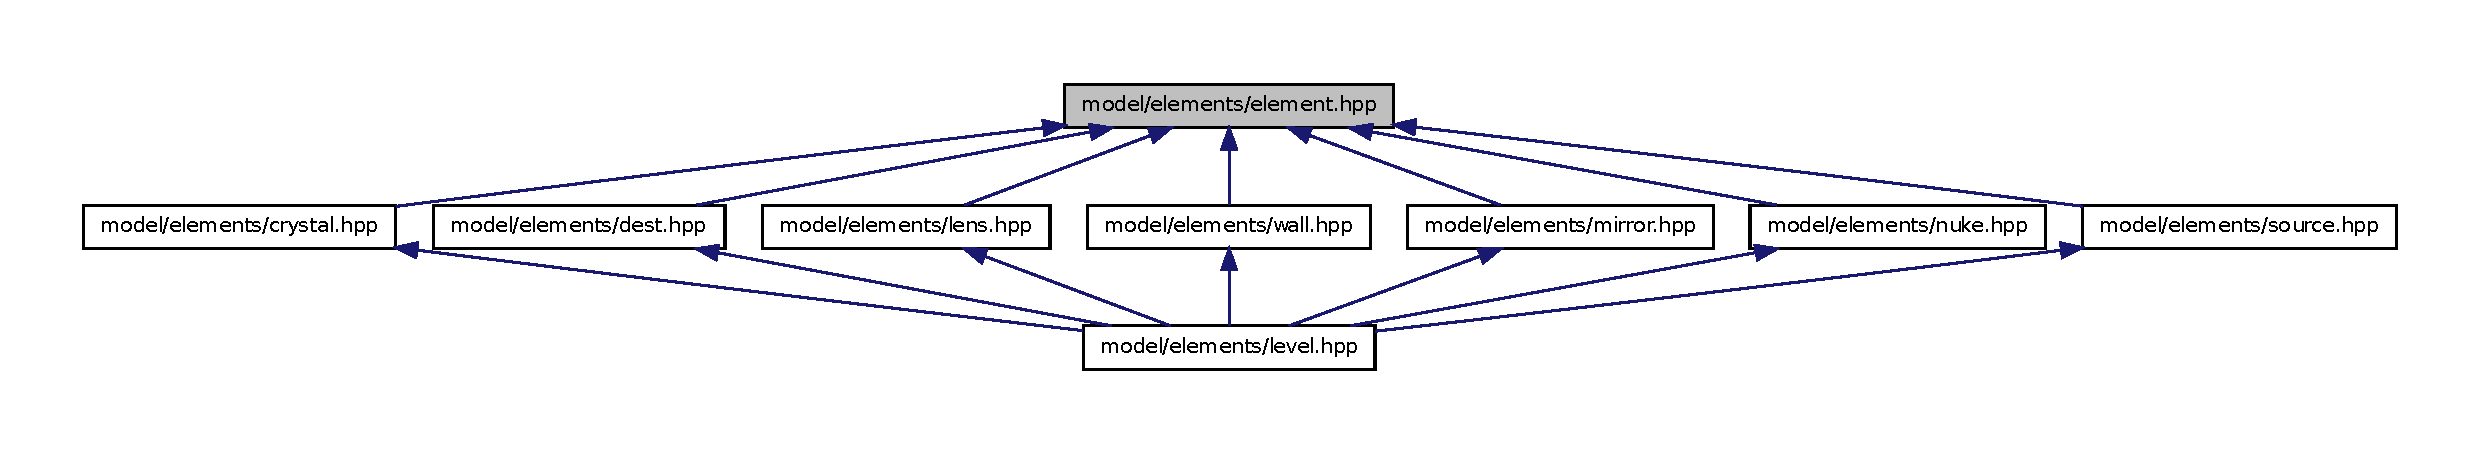
\includegraphics[width=350pt]{d9/d68/element_8hpp__dep__incl}
\end{center}
\end{figure}
\subsection*{Classes}
\begin{DoxyCompactItemize}
\item 
class \hyperlink{classElement}{Element}
\begin{DoxyCompactList}\small\item\em Un élément est un composant du jeu se devant de communiquer son état au niveau le gérant. \end{DoxyCompactList}\end{DoxyCompactItemize}

\hypertarget{lens_8hpp}{}\section{Référence du fichier model/elements/lens.hpp}
\label{lens_8hpp}\index{model/elements/lens.\+hpp@{model/elements/lens.\+hpp}}
{\ttfamily \#include $<$ostream$>$}\\*
{\ttfamily \#include \char`\"{}model/elements/element.\+hpp\char`\"{}}\\*
{\ttfamily \#include \char`\"{}model/geometry/ellipse.\+hpp\char`\"{}}\\*
{\ttfamily \#include \char`\"{}model/geometry/point.\+hpp\char`\"{}}\\*
Graphe des dépendances par inclusion de lens.\+hpp\+:\nopagebreak
\begin{figure}[H]
\begin{center}
\leavevmode
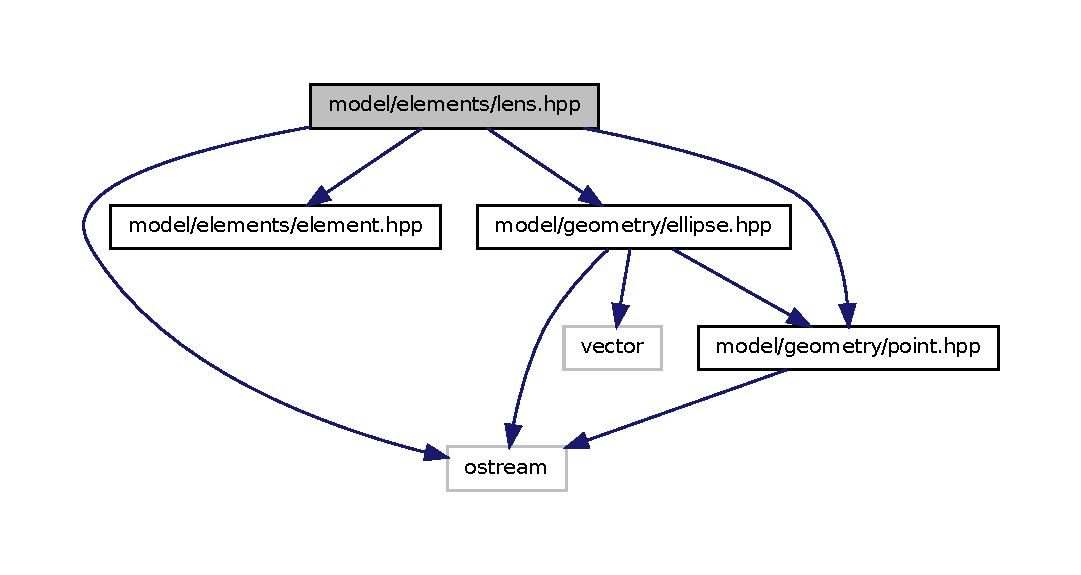
\includegraphics[width=350pt]{d5/dbe/lens_8hpp__incl}
\end{center}
\end{figure}
Ce graphe montre quels fichiers incluent directement ou indirectement ce fichier \+:\nopagebreak
\begin{figure}[H]
\begin{center}
\leavevmode
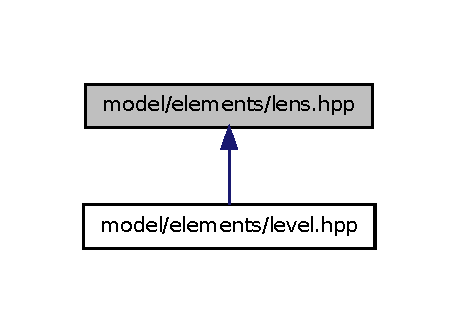
\includegraphics[width=220pt]{d1/de8/lens_8hpp__dep__incl}
\end{center}
\end{figure}
\subsection*{Classes}
\begin{DoxyCompactItemize}
\item 
class \hyperlink{classLens}{Lens}
\begin{DoxyCompactList}\small\item\em Cette classe modélise les lentilles utilisées dans le jeu. \end{DoxyCompactList}\end{DoxyCompactItemize}
\subsection*{Fonctions}
\begin{DoxyCompactItemize}
\item 
std\+::ostream \& \hyperlink{lens_8hpp_aac31c6bab8be32c25c4d08f9b83da0fa}{operator$<$$<$} (std\+::ostream \&, const \hyperlink{classLens}{Lens} \&)
\begin{DoxyCompactList}\small\item\em Définition, externe, de l\textquotesingle{}opérateur permettant de produire un affichage formaté. \end{DoxyCompactList}\end{DoxyCompactItemize}


\subsection{Documentation des fonctions}
\hypertarget{lens_8hpp_aac31c6bab8be32c25c4d08f9b83da0fa}{}\index{lens.\+hpp@{lens.\+hpp}!operator$<$$<$@{operator$<$$<$}}
\index{operator$<$$<$@{operator$<$$<$}!lens.\+hpp@{lens.\+hpp}}
\subsubsection[{operator$<$$<$(std\+::ostream \&, const Lens \&)}]{\setlength{\rightskip}{0pt plus 5cm}std\+::ostream\& operator$<$$<$ (
\begin{DoxyParamCaption}
\item[{std\+::ostream \&}]{, }
\item[{const {\bf Lens} \&}]{}
\end{DoxyParamCaption}
)}\label{lens_8hpp_aac31c6bab8be32c25c4d08f9b83da0fa}


Définition, externe, de l\textquotesingle{}opérateur permettant de produire un affichage formaté. 

\begin{DoxyReturn}{Renvoie}
Le ostream rempli de la chaine formatée représentant la \hyperlink{classLens}{Lens} en paramètre. 
\end{DoxyReturn}

\hypertarget{level_8hpp}{}\section{Référence du fichier model/elements/level.hpp}
\label{level_8hpp}\index{model/elements/level.\+hpp@{model/elements/level.\+hpp}}
{\ttfamily \#include $<$vector$>$}\\*
{\ttfamily \#include $<$map$>$}\\*
{\ttfamily \#include $<$string$>$}\\*
{\ttfamily \#include \char`\"{}model/exception/starlightexception.\+hpp\char`\"{}}\\*
{\ttfamily \#include \char`\"{}model/elements/wall.\+hpp\char`\"{}}\\*
{\ttfamily \#include \char`\"{}model/elements/mirror.\+hpp\char`\"{}}\\*
{\ttfamily \#include \char`\"{}model/elements/crystal.\+hpp\char`\"{}}\\*
{\ttfamily \#include \char`\"{}model/elements/lens.\+hpp\char`\"{}}\\*
{\ttfamily \#include \char`\"{}model/elements/nuke.\+hpp\char`\"{}}\\*
{\ttfamily \#include \char`\"{}model/elements/source.\+hpp\char`\"{}}\\*
{\ttfamily \#include \char`\"{}model/elements/dest.\+hpp\char`\"{}}\\*
{\ttfamily \#include \char`\"{}model/elements/ray.\+hpp\char`\"{}}\\*
{\ttfamily \#include \char`\"{}view/windows/levelview.\+hpp\char`\"{}}\\*
Graphe des dépendances par inclusion de level.\+hpp\+:\nopagebreak
\begin{figure}[H]
\begin{center}
\leavevmode
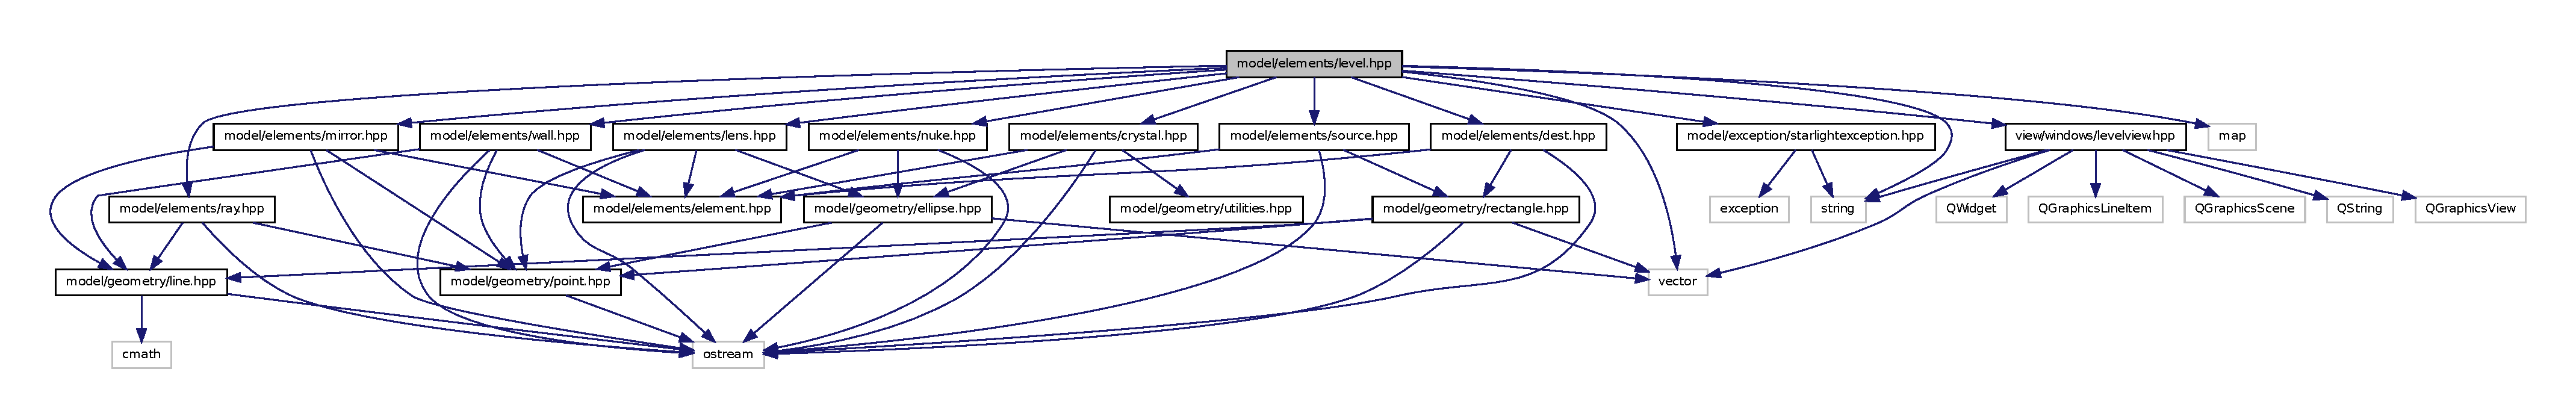
\includegraphics[width=350pt]{db/d47/level_8hpp__incl}
\end{center}
\end{figure}
\subsection*{Classes}
\begin{DoxyCompactItemize}
\item 
class \hyperlink{classLevel}{Level}
\begin{DoxyCompactList}\small\item\em Modélise une carte telle qu\textquotesingle{}utilisée dans le jeu. \end{DoxyCompactList}\end{DoxyCompactItemize}

\hypertarget{levelFactory_8hpp}{}\section{Référence du fichier model/elements/level\+Factory.hpp}
\label{levelFactory_8hpp}\index{model/elements/level\+Factory.\+hpp@{model/elements/level\+Factory.\+hpp}}
{\ttfamily \#include $<$fstream$>$}\\*
{\ttfamily \#include $<$sstream$>$}\\*
Graphe des dépendances par inclusion de level\+Factory.\+hpp\+:\nopagebreak
\begin{figure}[H]
\begin{center}
\leavevmode
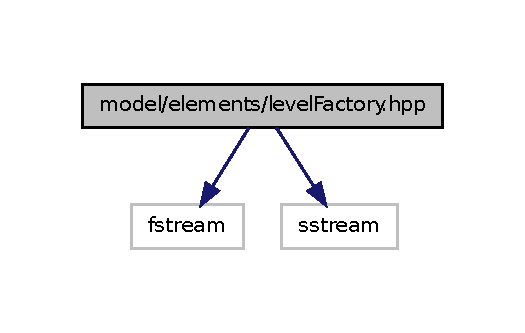
\includegraphics[width=252pt]{df/d8e/levelFactory_8hpp__incl}
\end{center}
\end{figure}
\subsection*{Espaces de nommage}
\begin{DoxyCompactItemize}
\item 
 \hyperlink{namespacelevelFactory}{level\+Factory}
\begin{DoxyCompactList}\small\item\em Fonctions utilitaires permettant divers éléments du jeu à partir d\textquotesingle{}un fichier .lvl. \end{DoxyCompactList}\end{DoxyCompactItemize}
\subsection*{Fonctions}
\begin{DoxyCompactItemize}
\item 
\hyperlink{classLevel}{Level} $\ast$ \hyperlink{namespacelevelFactory_a6f72186d33354f4f19b83f510e4bdb10}{level\+Factory\+::get\+Level\+From\+File} (std\+::string)
\begin{DoxyCompactList}\small\item\em Permet d\textquotesingle{}obtenir une référence vers une nouvelle carte initialisée à partir d\textquotesingle{}un fichier .level. \end{DoxyCompactList}\item 
\hyperlink{classSource}{Source} \hyperlink{namespacelevelFactory_ac9bd1e2b73944b567d2b454ad861efc0}{level\+Factory\+::get\+Source} (std\+::ifstream \&)
\begin{DoxyCompactList}\small\item\em Permet d\textquotesingle{} obtenir une source à partir d\textquotesingle{}un fichier .lvl déjà ouvert. \end{DoxyCompactList}\item 
\hyperlink{classDest}{Dest} \hyperlink{namespacelevelFactory_ab725f4fefde6c96197b6baf7c0eadfc7}{level\+Factory\+::get\+Destination} (std\+::ifstream \&)
\begin{DoxyCompactList}\small\item\em Permet d\textquotesingle{} obtenir une destination à partir d\textquotesingle{}un fichier .lvl déjà ouvert. \end{DoxyCompactList}\item 
\hyperlink{classCrystal}{Crystal} \hyperlink{namespacelevelFactory_a4a9434297ea3998d9466a0f11407c041}{level\+Factory\+::get\+Crystal} (std\+::ifstream \&)
\begin{DoxyCompactList}\small\item\em Permet d\textquotesingle{} obtenir un crystal à partir d\textquotesingle{}un fichier .lvl déjà ouvert. \end{DoxyCompactList}\item 
\hyperlink{classLens}{Lens} \hyperlink{namespacelevelFactory_a697af6e8eba86734063c0678c1b5b926}{level\+Factory\+::get\+Lens} (std\+::ifstream \&)
\begin{DoxyCompactList}\small\item\em Permet d\textquotesingle{} obtenir une lentille à partir d\textquotesingle{}un fichier .lvl déjà ouvert. \end{DoxyCompactList}\item 
\hyperlink{classWall}{Wall} \hyperlink{namespacelevelFactory_a94f4b8816d9893571a0cbd2fe55f3adf}{level\+Factory\+::get\+Wall} (std\+::ifstream \&)
\begin{DoxyCompactList}\small\item\em Permet d\textquotesingle{} obtenir un mur à partir d\textquotesingle{}un fichier .lvl déjà ouvert. \end{DoxyCompactList}\item 
\hyperlink{classNuke}{Nuke} \hyperlink{namespacelevelFactory_aa187b99195fd9d9106eaf8b6ac3b6809}{level\+Factory\+::get\+Nuke} (std\+::ifstream \&)
\begin{DoxyCompactList}\small\item\em Permet d\textquotesingle{} obtenir une bombe à partir d\textquotesingle{}un fichier .lvl déjà ouvert. \end{DoxyCompactList}\item 
\hyperlink{classMirror}{Mirror} \hyperlink{namespacelevelFactory_a9e17b53fc85131232092e428a2f0c803}{level\+Factory\+::get\+Mirror} (std\+::ifstream \&)
\begin{DoxyCompactList}\small\item\em Permet d\textquotesingle{} obtenir un mirroir à partir d\textquotesingle{}un fichier .lvl déjà ouvert. \end{DoxyCompactList}\end{DoxyCompactItemize}

\hypertarget{mirror_8hpp}{}\section{Référence du fichier model/elements/mirror.hpp}
\label{mirror_8hpp}\index{model/elements/mirror.\+hpp@{model/elements/mirror.\+hpp}}
{\ttfamily \#include $<$ostream$>$}\\*
{\ttfamily \#include \char`\"{}model/elements/element.\+hpp\char`\"{}}\\*
{\ttfamily \#include \char`\"{}model/geometry/line.\+hpp\char`\"{}}\\*
{\ttfamily \#include \char`\"{}model/geometry/point.\+hpp\char`\"{}}\\*
Graphe des dépendances par inclusion de mirror.\+hpp\+:\nopagebreak
\begin{figure}[H]
\begin{center}
\leavevmode
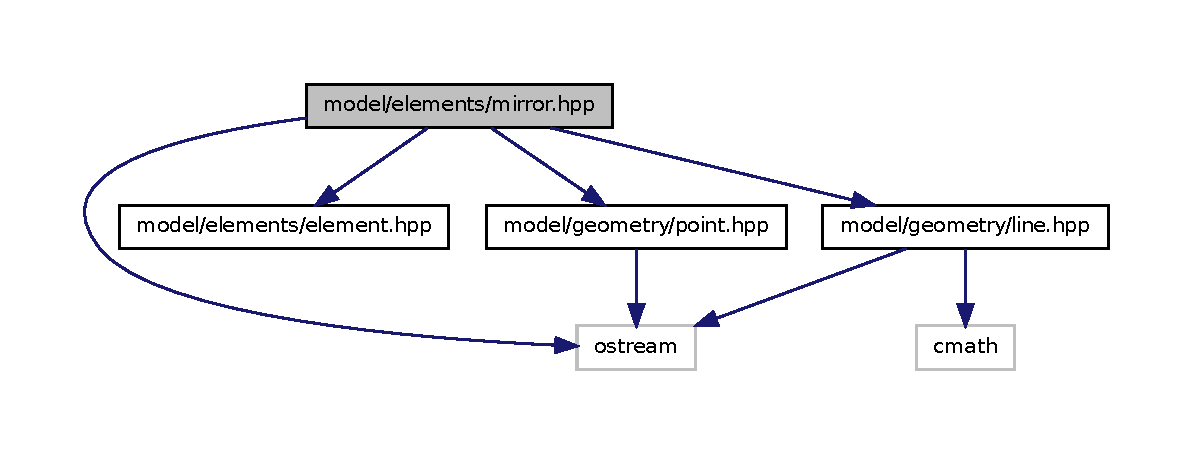
\includegraphics[width=350pt]{d8/dc2/mirror_8hpp__incl}
\end{center}
\end{figure}
Ce graphe montre quels fichiers incluent directement ou indirectement ce fichier \+:\nopagebreak
\begin{figure}[H]
\begin{center}
\leavevmode
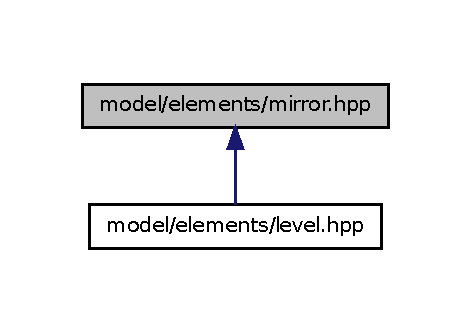
\includegraphics[width=226pt]{d8/d81/mirror_8hpp__dep__incl}
\end{center}
\end{figure}
\subsection*{Classes}
\begin{DoxyCompactItemize}
\item 
class \hyperlink{classMirror}{Mirror}
\begin{DoxyCompactList}\small\item\em Cette classe modélise les miroirs utilisés dans le jeu. \end{DoxyCompactList}\end{DoxyCompactItemize}
\subsection*{Fonctions}
\begin{DoxyCompactItemize}
\item 
std\+::ostream \& \hyperlink{mirror_8hpp_a740b4bd02874d74283d81e1f4fd9c055}{operator$<$$<$} (std\+::ostream \&, const \hyperlink{classMirror}{Mirror} \&)
\begin{DoxyCompactList}\small\item\em Définition, externe, de l\textquotesingle{}opérateur permettant de produire un affichage formaté. \end{DoxyCompactList}\end{DoxyCompactItemize}


\subsection{Documentation des fonctions}
\hypertarget{mirror_8hpp_a740b4bd02874d74283d81e1f4fd9c055}{}\index{mirror.\+hpp@{mirror.\+hpp}!operator$<$$<$@{operator$<$$<$}}
\index{operator$<$$<$@{operator$<$$<$}!mirror.\+hpp@{mirror.\+hpp}}
\subsubsection[{operator$<$$<$(std\+::ostream \&, const Mirror \&)}]{\setlength{\rightskip}{0pt plus 5cm}std\+::ostream\& operator$<$$<$ (
\begin{DoxyParamCaption}
\item[{std\+::ostream \&}]{, }
\item[{const {\bf Mirror} \&}]{}
\end{DoxyParamCaption}
)}\label{mirror_8hpp_a740b4bd02874d74283d81e1f4fd9c055}


Définition, externe, de l\textquotesingle{}opérateur permettant de produire un affichage formaté. 

\begin{DoxyReturn}{Renvoie}
Le ostream rempli de la chaine formatée représentant le \hyperlink{classMirror}{Mirror} en paramètre. 
\end{DoxyReturn}

\hypertarget{nuke_8hpp}{}\section{Référence du fichier model/elements/nuke.hpp}
\label{nuke_8hpp}\index{model/elements/nuke.\+hpp@{model/elements/nuke.\+hpp}}
{\ttfamily \#include $<$ostream$>$}\\*
{\ttfamily \#include \char`\"{}model/elements/element.\+hpp\char`\"{}}\\*
{\ttfamily \#include \char`\"{}model/geometry/ellipse.\+hpp\char`\"{}}\\*
Graphe des dépendances par inclusion de nuke.\+hpp\+:\nopagebreak
\begin{figure}[H]
\begin{center}
\leavevmode
\includegraphics[width=350pt]{d8/df5/nuke_8hpp__incl}
\end{center}
\end{figure}
Ce graphe montre quels fichiers incluent directement ou indirectement ce fichier \+:\nopagebreak
\begin{figure}[H]
\begin{center}
\leavevmode
\includegraphics[width=222pt]{d7/de5/nuke_8hpp__dep__incl}
\end{center}
\end{figure}
\subsection*{Classes}
\begin{DoxyCompactItemize}
\item 
class \hyperlink{classNuke}{Nuke}
\begin{DoxyCompactList}\small\item\em Cette classe modélise les bombes utilisées dans le jeu. \end{DoxyCompactList}\end{DoxyCompactItemize}
\subsection*{Fonctions}
\begin{DoxyCompactItemize}
\item 
std\+::ostream \& \hyperlink{nuke_8hpp_a02952d325ff13788622fcd80a217b7b0}{operator$<$$<$} (std\+::ostream \&, const \hyperlink{classNuke}{Nuke} \&)
\begin{DoxyCompactList}\small\item\em Définition, externe, de l\textquotesingle{}opérateur permettant de produire un affichage formaté. \end{DoxyCompactList}\end{DoxyCompactItemize}


\subsection{Documentation des fonctions}
\hypertarget{nuke_8hpp_a02952d325ff13788622fcd80a217b7b0}{}\index{nuke.\+hpp@{nuke.\+hpp}!operator$<$$<$@{operator$<$$<$}}
\index{operator$<$$<$@{operator$<$$<$}!nuke.\+hpp@{nuke.\+hpp}}
\subsubsection[{operator$<$$<$(std\+::ostream \&, const Nuke \&)}]{\setlength{\rightskip}{0pt plus 5cm}std\+::ostream\& operator$<$$<$ (
\begin{DoxyParamCaption}
\item[{std\+::ostream \&}]{, }
\item[{const {\bf Nuke} \&}]{}
\end{DoxyParamCaption}
)}\label{nuke_8hpp_a02952d325ff13788622fcd80a217b7b0}


Définition, externe, de l\textquotesingle{}opérateur permettant de produire un affichage formaté. 

\begin{DoxyReturn}{Renvoie}
Le ostream rempli de la chaine formatée représentant le \hyperlink{classNuke}{Nuke} en paramètre. 
\end{DoxyReturn}

\hypertarget{ray_8hpp}{}\section{Référence du fichier model/elements/ray.hpp}
\label{ray_8hpp}\index{model/elements/ray.\+hpp@{model/elements/ray.\+hpp}}
{\ttfamily \#include $<$ostream$>$}\\*
{\ttfamily \#include \char`\"{}model/geometry/point.\+hpp\char`\"{}}\\*
{\ttfamily \#include \char`\"{}model/geometry/line.\+hpp\char`\"{}}\\*
Graphe des dépendances par inclusion de ray.\+hpp\+:\nopagebreak
\begin{figure}[H]
\begin{center}
\leavevmode
\includegraphics[width=350pt]{de/d63/ray_8hpp__incl}
\end{center}
\end{figure}
Ce graphe montre quels fichiers incluent directement ou indirectement ce fichier \+:\nopagebreak
\begin{figure}[H]
\begin{center}
\leavevmode
\includegraphics[width=220pt]{d3/da1/ray_8hpp__dep__incl}
\end{center}
\end{figure}
\subsection*{Classes}
\begin{DoxyCompactItemize}
\item 
class \hyperlink{classRay}{Ray}
\begin{DoxyCompactList}\small\item\em Cette classe modélise les rayons lumineux, concept central du jeu. \end{DoxyCompactList}\end{DoxyCompactItemize}
\subsection*{Fonctions}
\begin{DoxyCompactItemize}
\item 
std\+::ostream \& \hyperlink{ray_8hpp_a7b5ecffe445197eba7b60509bc488f87}{operator$<$$<$} (std\+::ostream \&, const \hyperlink{classRay}{Ray} \&)
\begin{DoxyCompactList}\small\item\em Définition, externe, de l\textquotesingle{}opérateur permettant de produire un affichage formaté. \end{DoxyCompactList}\end{DoxyCompactItemize}


\subsection{Documentation des fonctions}
\hypertarget{ray_8hpp_a7b5ecffe445197eba7b60509bc488f87}{}\index{ray.\+hpp@{ray.\+hpp}!operator$<$$<$@{operator$<$$<$}}
\index{operator$<$$<$@{operator$<$$<$}!ray.\+hpp@{ray.\+hpp}}
\subsubsection[{operator$<$$<$(std\+::ostream \&, const Ray \&)}]{\setlength{\rightskip}{0pt plus 5cm}std\+::ostream\& operator$<$$<$ (
\begin{DoxyParamCaption}
\item[{std\+::ostream \&}]{, }
\item[{const {\bf Ray} \&}]{}
\end{DoxyParamCaption}
)}\label{ray_8hpp_a7b5ecffe445197eba7b60509bc488f87}


Définition, externe, de l\textquotesingle{}opérateur permettant de produire un affichage formaté. 

\begin{DoxyReturn}{Renvoie}
Le ostream rempli de la chaine formatée représentant le \hyperlink{classRay}{Ray} en paramètre. 
\end{DoxyReturn}

\hypertarget{source_8hpp}{}\section{Référence du fichier model/elements/source.hpp}
\label{source_8hpp}\index{model/elements/source.\+hpp@{model/elements/source.\+hpp}}
{\ttfamily \#include $<$ostream$>$}\\*
{\ttfamily \#include \char`\"{}model/geometry/rectangle.\+hpp\char`\"{}}\\*
{\ttfamily \#include \char`\"{}model/elements/element.\+hpp\char`\"{}}\\*
Graphe des dépendances par inclusion de source.\+hpp\+:\nopagebreak
\begin{figure}[H]
\begin{center}
\leavevmode
\includegraphics[width=350pt]{d4/d2f/source_8hpp__incl}
\end{center}
\end{figure}
Ce graphe montre quels fichiers incluent directement ou indirectement ce fichier \+:\nopagebreak
\begin{figure}[H]
\begin{center}
\leavevmode
\includegraphics[width=230pt]{d2/dd0/source_8hpp__dep__incl}
\end{center}
\end{figure}
\subsection*{Classes}
\begin{DoxyCompactItemize}
\item 
class \hyperlink{classSource}{Source}
\begin{DoxyCompactList}\small\item\em Modélise la source lumineuse utilisée dans le jeu. \end{DoxyCompactList}\end{DoxyCompactItemize}
\subsection*{Fonctions}
\begin{DoxyCompactItemize}
\item 
std\+::ostream \& \hyperlink{source_8hpp_acd9238357b3489d23520d209f3447eda}{operator$<$$<$} (std\+::ostream \&, const \hyperlink{classSource}{Source} \&)
\begin{DoxyCompactList}\small\item\em Définition, externe, de l\textquotesingle{}opérateur permettant de produire un affichage formaté. \end{DoxyCompactList}\end{DoxyCompactItemize}


\subsection{Documentation des fonctions}
\hypertarget{source_8hpp_acd9238357b3489d23520d209f3447eda}{}\index{source.\+hpp@{source.\+hpp}!operator$<$$<$@{operator$<$$<$}}
\index{operator$<$$<$@{operator$<$$<$}!source.\+hpp@{source.\+hpp}}
\subsubsection[{operator$<$$<$(std\+::ostream \&, const Source \&)}]{\setlength{\rightskip}{0pt plus 5cm}std\+::ostream\& operator$<$$<$ (
\begin{DoxyParamCaption}
\item[{std\+::ostream \&}]{, }
\item[{const {\bf Source} \&}]{}
\end{DoxyParamCaption}
)}\label{source_8hpp_acd9238357b3489d23520d209f3447eda}


Définition, externe, de l\textquotesingle{}opérateur permettant de produire un affichage formaté. 

\begin{DoxyReturn}{Renvoie}
Le ostream rempli de la chaine formatée représentant la \hyperlink{classSource}{Source} en paramètre. 
\end{DoxyReturn}

\hypertarget{wall_8hpp}{}\section{Référence du fichier model/elements/wall.hpp}
\label{wall_8hpp}\index{model/elements/wall.\+hpp@{model/elements/wall.\+hpp}}
{\ttfamily \#include $<$ostream$>$}\\*
{\ttfamily \#include \char`\"{}model/geometry/line.\+hpp\char`\"{}}\\*
{\ttfamily \#include \char`\"{}model/elements/element.\+hpp\char`\"{}}\\*
{\ttfamily \#include \char`\"{}model/geometry/point.\+hpp\char`\"{}}\\*
Graphe des dépendances par inclusion de wall.\+hpp\+:\nopagebreak
\begin{figure}[H]
\begin{center}
\leavevmode
\includegraphics[width=350pt]{d3/d25/wall_8hpp__incl}
\end{center}
\end{figure}
Ce graphe montre quels fichiers incluent directement ou indirectement ce fichier \+:\nopagebreak
\begin{figure}[H]
\begin{center}
\leavevmode
\includegraphics[width=220pt]{d6/dd2/wall_8hpp__dep__incl}
\end{center}
\end{figure}
\subsection*{Classes}
\begin{DoxyCompactItemize}
\item 
class \hyperlink{classWall}{Wall}
\begin{DoxyCompactList}\small\item\em Cette classe modélise les murs utilisés dans le jeu. \end{DoxyCompactList}\end{DoxyCompactItemize}
\subsection*{Fonctions}
\begin{DoxyCompactItemize}
\item 
std\+::ostream \& \hyperlink{wall_8hpp_a762127d24b7c3e98f9da57702f628a78}{operator$<$$<$} (std\+::ostream \&, const \hyperlink{classWall}{Wall} \&)
\begin{DoxyCompactList}\small\item\em Définition, externe, de l\textquotesingle{}opérateur permettant de produire un affichage formaté. \end{DoxyCompactList}\end{DoxyCompactItemize}


\subsection{Documentation des fonctions}
\hypertarget{wall_8hpp_a762127d24b7c3e98f9da57702f628a78}{}\index{wall.\+hpp@{wall.\+hpp}!operator$<$$<$@{operator$<$$<$}}
\index{operator$<$$<$@{operator$<$$<$}!wall.\+hpp@{wall.\+hpp}}
\subsubsection[{operator$<$$<$(std\+::ostream \&, const Wall \&)}]{\setlength{\rightskip}{0pt plus 5cm}std\+::ostream\& operator$<$$<$ (
\begin{DoxyParamCaption}
\item[{std\+::ostream \&}]{, }
\item[{const {\bf Wall} \&}]{}
\end{DoxyParamCaption}
)}\label{wall_8hpp_a762127d24b7c3e98f9da57702f628a78}


Définition, externe, de l\textquotesingle{}opérateur permettant de produire un affichage formaté. 

\begin{DoxyReturn}{Renvoie}
Le ostream rempli de la chaine formatée représentant le \hyperlink{classWall}{Wall} en paramètre. 
\end{DoxyReturn}

\hypertarget{starlightexception_8hpp}{}\section{Référence du fichier model/exception/starlightexception.hpp}
\label{starlightexception_8hpp}\index{model/exception/starlightexception.\+hpp@{model/exception/starlightexception.\+hpp}}
{\ttfamily \#include $<$exception$>$}\\*
{\ttfamily \#include $<$string$>$}\\*
Graphe des dépendances par inclusion de starlightexception.\+hpp\+:\nopagebreak
\begin{figure}[H]
\begin{center}
\leavevmode
\includegraphics[width=286pt]{d5/d15/starlightexception_8hpp__incl}
\end{center}
\end{figure}
Ce graphe montre quels fichiers incluent directement ou indirectement ce fichier \+:\nopagebreak
\begin{figure}[H]
\begin{center}
\leavevmode
\includegraphics[width=286pt]{d6/d3c/starlightexception_8hpp__dep__incl}
\end{center}
\end{figure}
\subsection*{Classes}
\begin{DoxyCompactItemize}
\item 
class \hyperlink{classStarlightException}{Starlight\+Exception}
\begin{DoxyCompactList}\small\item\em Cette classe représente une exception spécifique au jeu Starlight. \end{DoxyCompactList}\end{DoxyCompactItemize}

\hypertarget{ellipse_8hpp}{}\section{Référence du fichier model/geometry/ellipse.hpp}
\label{ellipse_8hpp}\index{model/geometry/ellipse.\+hpp@{model/geometry/ellipse.\+hpp}}
{\ttfamily \#include $<$vector$>$}\\*
{\ttfamily \#include $<$ostream$>$}\\*
{\ttfamily \#include \char`\"{}model/geometry/point.\+hpp\char`\"{}}\\*
Graphe des dépendances par inclusion de ellipse.\+hpp\+:\nopagebreak
\begin{figure}[H]
\begin{center}
\leavevmode
\includegraphics[width=327pt]{d4/df3/ellipse_8hpp__incl}
\end{center}
\end{figure}
Ce graphe montre quels fichiers incluent directement ou indirectement ce fichier \+:\nopagebreak
\begin{figure}[H]
\begin{center}
\leavevmode
\includegraphics[width=350pt]{d3/d48/ellipse_8hpp__dep__incl}
\end{center}
\end{figure}
\subsection*{Classes}
\begin{DoxyCompactItemize}
\item 
class \hyperlink{classEllipse}{Ellipse}
\begin{DoxyCompactList}\small\item\em Représente un cercle sous la forme; $ circle \equiv x^2/xRadius + y^2/yRadius = 1 $. \end{DoxyCompactList}\end{DoxyCompactItemize}
\subsection*{Fonctions}
\begin{DoxyCompactItemize}
\item 
std\+::ostream \& \hyperlink{ellipse_8hpp_af6dc987f9c8dc6d36ddf435fd16971fe}{operator$<$$<$} (std\+::ostream \&, const \hyperlink{classEllipse}{Ellipse} \&)
\begin{DoxyCompactList}\small\item\em Définition, externe, de l\textquotesingle{}opérateur permettant de produire un affichage formaté. \end{DoxyCompactList}\end{DoxyCompactItemize}


\subsection{Documentation des fonctions}
\hypertarget{ellipse_8hpp_af6dc987f9c8dc6d36ddf435fd16971fe}{}\index{ellipse.\+hpp@{ellipse.\+hpp}!operator$<$$<$@{operator$<$$<$}}
\index{operator$<$$<$@{operator$<$$<$}!ellipse.\+hpp@{ellipse.\+hpp}}
\subsubsection[{operator$<$$<$(std\+::ostream \&, const Ellipse \&)}]{\setlength{\rightskip}{0pt plus 5cm}std\+::ostream\& operator$<$$<$ (
\begin{DoxyParamCaption}
\item[{std\+::ostream \&}]{, }
\item[{const {\bf Ellipse} \&}]{}
\end{DoxyParamCaption}
)}\label{ellipse_8hpp_af6dc987f9c8dc6d36ddf435fd16971fe}


Définition, externe, de l\textquotesingle{}opérateur permettant de produire un affichage formaté. 

\begin{DoxyReturn}{Renvoie}
Le ostream rempli de la chaine formatée représentant l\textquotesingle{}ellipse en paramètre. 
\end{DoxyReturn}

\hypertarget{line_8hpp}{}\section{Référence du fichier model/geometry/line.hpp}
\label{line_8hpp}\index{model/geometry/line.\+hpp@{model/geometry/line.\+hpp}}
{\ttfamily \#include $<$cmath$>$}\\*
{\ttfamily \#include $<$ostream$>$}\\*
Graphe des dépendances par inclusion de line.\+hpp\+:\nopagebreak
\begin{figure}[H]
\begin{center}
\leavevmode
\includegraphics[width=216pt]{d8/de5/line_8hpp__incl}
\end{center}
\end{figure}
Ce graphe montre quels fichiers incluent directement ou indirectement ce fichier \+:\nopagebreak
\begin{figure}[H]
\begin{center}
\leavevmode
\includegraphics[width=350pt]{d3/dc1/line_8hpp__dep__incl}
\end{center}
\end{figure}
\subsection*{Classes}
\begin{DoxyCompactItemize}
\item 
class \hyperlink{classLine}{Line}
\begin{DoxyCompactList}\small\item\em Représente une droite sous la forme de son équation complète; $ eq \equiv y = slope \cdot x + indepTerm $. \end{DoxyCompactList}\end{DoxyCompactItemize}
\subsection*{Fonctions}
\begin{DoxyCompactItemize}
\item 
std\+::ostream \& \hyperlink{line_8hpp_a97d3a21266ef8f4299bcba875f45399a}{operator$<$$<$} (std\+::ostream \&, const \hyperlink{classLine}{Line} \&)
\begin{DoxyCompactList}\small\item\em Définition, externe, de l\textquotesingle{}opérateur permettant de produire un affichage formaté. \end{DoxyCompactList}\end{DoxyCompactItemize}


\subsection{Documentation des fonctions}
\hypertarget{line_8hpp_a97d3a21266ef8f4299bcba875f45399a}{}\index{line.\+hpp@{line.\+hpp}!operator$<$$<$@{operator$<$$<$}}
\index{operator$<$$<$@{operator$<$$<$}!line.\+hpp@{line.\+hpp}}
\subsubsection[{operator$<$$<$(std\+::ostream \&, const Line \&)}]{\setlength{\rightskip}{0pt plus 5cm}std\+::ostream\& operator$<$$<$ (
\begin{DoxyParamCaption}
\item[{std\+::ostream \&}]{, }
\item[{const {\bf Line} \&}]{}
\end{DoxyParamCaption}
)}\label{line_8hpp_a97d3a21266ef8f4299bcba875f45399a}


Définition, externe, de l\textquotesingle{}opérateur permettant de produire un affichage formaté. 

\begin{DoxyReturn}{Renvoie}
Le ostream rempli de la chaine formatée représentant la Ligne en paramètre. 
\end{DoxyReturn}

\hypertarget{point_8hpp}{}\section{Référence du fichier model/geometry/point.hpp}
\label{point_8hpp}\index{model/geometry/point.\+hpp@{model/geometry/point.\+hpp}}
{\ttfamily \#include $<$ostream$>$}\\*
Graphe des dépendances par inclusion de point.\+hpp\+:\nopagebreak
\begin{figure}[H]
\begin{center}
\leavevmode
\includegraphics[width=224pt]{d7/db6/point_8hpp__incl}
\end{center}
\end{figure}
Ce graphe montre quels fichiers incluent directement ou indirectement ce fichier \+:\nopagebreak
\begin{figure}[H]
\begin{center}
\leavevmode
\includegraphics[width=350pt]{d6/d56/point_8hpp__dep__incl}
\end{center}
\end{figure}
\subsection*{Classes}
\begin{DoxyCompactItemize}
\item 
class \hyperlink{classPoint}{Point}
\begin{DoxyCompactList}\small\item\em Cette classe modélise un point de coordonnés dans le plan $ R^2 $ sous deux formes \+: \end{DoxyCompactList}\end{DoxyCompactItemize}
\subsection*{Fonctions}
\begin{DoxyCompactItemize}
\item 
std\+::ostream \& \hyperlink{point_8hpp_ad1a23220347abf8f0b797b38165be717}{operator$<$$<$} (std\+::ostream \&, const \hyperlink{classPoint}{Point} \&)
\begin{DoxyCompactList}\small\item\em Définition, externe, de l\textquotesingle{}opérateur permettant de produire un affichage formaté. \end{DoxyCompactList}\end{DoxyCompactItemize}


\subsection{Documentation des fonctions}
\hypertarget{point_8hpp_ad1a23220347abf8f0b797b38165be717}{}\index{point.\+hpp@{point.\+hpp}!operator$<$$<$@{operator$<$$<$}}
\index{operator$<$$<$@{operator$<$$<$}!point.\+hpp@{point.\+hpp}}
\subsubsection[{operator$<$$<$(std\+::ostream \&, const Point \&)}]{\setlength{\rightskip}{0pt plus 5cm}std\+::ostream\& operator$<$$<$ (
\begin{DoxyParamCaption}
\item[{std\+::ostream \&}]{, }
\item[{const {\bf Point} \&}]{}
\end{DoxyParamCaption}
)}\label{point_8hpp_ad1a23220347abf8f0b797b38165be717}


Définition, externe, de l\textquotesingle{}opérateur permettant de produire un affichage formaté. 

\begin{DoxyReturn}{Renvoie}
Le ostream rempli de la chaine formatée représentant le \hyperlink{classPoint}{Point} en paramètre. 
\end{DoxyReturn}

\hypertarget{rectangle_8hpp}{}\section{Référence du fichier model/geometry/rectangle.hpp}
\label{rectangle_8hpp}\index{model/geometry/rectangle.\+hpp@{model/geometry/rectangle.\+hpp}}
{\ttfamily \#include $<$vector$>$}\\*
{\ttfamily \#include $<$ostream$>$}\\*
{\ttfamily \#include \char`\"{}model/geometry/point.\+hpp\char`\"{}}\\*
{\ttfamily \#include \char`\"{}model/geometry/line.\+hpp\char`\"{}}\\*
Graphe des dépendances par inclusion de rectangle.\+hpp\+:\nopagebreak
\begin{figure}[H]
\begin{center}
\leavevmode
\includegraphics[width=350pt]{da/d1a/rectangle_8hpp__incl}
\end{center}
\end{figure}
Ce graphe montre quels fichiers incluent directement ou indirectement ce fichier \+:\nopagebreak
\begin{figure}[H]
\begin{center}
\leavevmode
\includegraphics[width=350pt]{dd/d0d/rectangle_8hpp__dep__incl}
\end{center}
\end{figure}
\subsection*{Classes}
\begin{DoxyCompactItemize}
\item 
class \hyperlink{classRectangle}{Rectangle}
\begin{DoxyCompactList}\small\item\em Le rectangle est objet géométrique, du plan, à quatre coté parallèles deux à deux. \end{DoxyCompactList}\end{DoxyCompactItemize}
\subsection*{Fonctions}
\begin{DoxyCompactItemize}
\item 
std\+::ostream \& \hyperlink{rectangle_8hpp_add53d343a030dfbfaa4bed7d92add354}{operator$<$$<$} (std\+::ostream \&, const \hyperlink{classRectangle}{Rectangle} \&)
\begin{DoxyCompactList}\small\item\em Définition, externe, de l\textquotesingle{}opérateur permettant de produire un affichage formaté. \end{DoxyCompactList}\end{DoxyCompactItemize}


\subsection{Documentation des fonctions}
\hypertarget{rectangle_8hpp_add53d343a030dfbfaa4bed7d92add354}{}\index{rectangle.\+hpp@{rectangle.\+hpp}!operator$<$$<$@{operator$<$$<$}}
\index{operator$<$$<$@{operator$<$$<$}!rectangle.\+hpp@{rectangle.\+hpp}}
\subsubsection[{operator$<$$<$(std\+::ostream \&, const Rectangle \&)}]{\setlength{\rightskip}{0pt plus 5cm}std\+::ostream\& operator$<$$<$ (
\begin{DoxyParamCaption}
\item[{std\+::ostream \&}]{, }
\item[{const {\bf Rectangle} \&}]{}
\end{DoxyParamCaption}
)}\label{rectangle_8hpp_add53d343a030dfbfaa4bed7d92add354}


Définition, externe, de l\textquotesingle{}opérateur permettant de produire un affichage formaté. 

\begin{DoxyReturn}{Renvoie}
Le ostream rempli de la chaine formatée représentant le \hyperlink{classRectangle}{Rectangle} en paramètre. 
\end{DoxyReturn}

\hypertarget{utilities_8hpp}{}\section{Référence du fichier model/geometry/utilities.hpp}
\label{utilities_8hpp}\index{model/geometry/utilities.\+hpp@{model/geometry/utilities.\+hpp}}
Ce graphe montre quels fichiers incluent directement ou indirectement ce fichier \+:\nopagebreak
\begin{figure}[H]
\begin{center}
\leavevmode
\includegraphics[width=234pt]{db/d84/utilities_8hpp__dep__incl}
\end{center}
\end{figure}
\subsection*{Espaces de nommage}
\begin{DoxyCompactItemize}
\item 
 \hyperlink{namespaceutilities}{utilities}
\begin{DoxyCompactList}\small\item\em Diverse fonctions utilitaires de géométrie. \end{DoxyCompactList}\end{DoxyCompactItemize}
\subsection*{Fonctions}
\begin{DoxyCompactItemize}
\item 
bool \hyperlink{namespaceutilities_a040360cbd22e36e7d8e399b553217242}{utilities\+::second\+Degree\+Equation\+Solver} (double, double, double, double $\ast$, double $\ast$)
\begin{DoxyCompactList}\small\item\em Permet de trouver les racines (si elles existe) d\textquotesingle{}une fonction du deuxième degré de forme $ax² + bx + c$. \end{DoxyCompactList}\item 
double \hyperlink{namespaceutilities_aa2ec82a874dad6aae298db007bc0aef6}{utilities\+::radian\+As\+Degree} (const double)
\begin{DoxyCompactList}\small\item\em Permet de trouver l\textquotesingle{}angle en degré d\textquotesingle{}un angle en radian. \end{DoxyCompactList}\item 
double \hyperlink{namespaceutilities_a743a501d731442689287e6306e01c2d4}{utilities\+::radian\+As\+Degree0to360} (const double)
\begin{DoxyCompactList}\small\item\em Permet de trouver l\textquotesingle{}angle en degré, entre 0 et 360, d\textquotesingle{}un angle en radian. \end{DoxyCompactList}\item 
bool \hyperlink{namespaceutilities_a30b551fcbf5672117358b7b660d5dbf1}{utilities\+::equals} (const double, const double, const double=\hyperlink{namespaceutilities_adf3b0db93e9d9a6057599d3629607c72}{utilities\+::\+E\+P\+S\+I\+L\+O\+N})
\begin{DoxyCompactList}\small\item\em Cette méthode permet de savoir si deux double sont égaux avec une marge d\textquotesingle{}erreur Epsilon passée en paramètre ou imposée par défaut à $ \epsilon = 10^{-7}$. \end{DoxyCompactList}\item 
int \hyperlink{namespaceutilities_a00ae09dc5ce4274969a2a28607426eb5}{utilities\+::round} (const double)
\begin{DoxyCompactList}\small\item\em Cette méthode cast un double en int on l\textquotesingle{}ayant au préalable arrondi à l\textquotesingle{}unité la plus proche (0.\+5). \end{DoxyCompactList}\item 
bool \hyperlink{namespaceutilities_a4001cf523b54a14a53b11938a2605964}{utilities\+::greater\+Or\+Equals} (const double, const double, const double=\hyperlink{namespaceutilities_adf3b0db93e9d9a6057599d3629607c72}{utilities\+::\+E\+P\+S\+I\+L\+O\+N})
\begin{DoxyCompactList}\small\item\em Cette méthode permet de vérifier l\textquotesingle{}inégalité $ nb_1 \geq nb_2 $ sur deux nombres réels avec une marge d\textquotesingle{}erreur Epsilon passée en paramètre ou imposée par défaut à $ \epsilon = 10^{-7}$. \end{DoxyCompactList}\item 
bool \hyperlink{namespaceutilities_a5b52313a89eff9ec934ab4e1fcf23be7}{utilities\+::less\+Or\+Equals} (const double, const double, const double=\hyperlink{namespaceutilities_adf3b0db93e9d9a6057599d3629607c72}{utilities\+::\+E\+P\+S\+I\+L\+O\+N})
\begin{DoxyCompactList}\small\item\em Cette méthode permet de vérifier l\textquotesingle{}inégalité $ nb_1 \leq nb_2 $ sur deux nombres réels avec une marge d\textquotesingle{}erreur Epsilon passée en paramètre ou imposée par défaut à $ \epsilon = 10^{-7}$. \end{DoxyCompactList}\item 
double \hyperlink{namespaceutilities_a6502e590807ff5ce206bf28b156c2d9e}{utilities\+::degree\+To\+Radian} (const double)
\begin{DoxyCompactList}\small\item\em Cette méthode permet de transformer des degrés en radian. \end{DoxyCompactList}\item 
double \hyperlink{namespaceutilities_a8ec19db42cc8962662eee53be6c6088d}{utilities\+::slope\+From\+Points} (const \hyperlink{classPoint}{Point} \&, const \hyperlink{classPoint}{Point} \&)
\begin{DoxyCompactList}\small\item\em Permet de trouver la pente d\textquotesingle{}une droite formée par deux points. \end{DoxyCompactList}\item 
bool \hyperlink{namespaceutilities_a41bdf53d6ca758ab77ab736b41ae272f}{utilities\+::is\+Half\+Pi\+Plus\+N\+Pi} (const double)
\begin{DoxyCompactList}\small\item\em Permet de savoir si l\textquotesingle{}angle, en radian, vaut $ \frac{\pi}{2} + n \cdot (2 \cdot \pi)$. \end{DoxyCompactList}\item 
double \hyperlink{namespaceutilities_a376cfb5f6c163526c76d1df2bcfe98d9}{utilities\+::tan} (const double)
\begin{DoxyCompactList}\small\item\em Permet d\textquotesingle{}avoir la valeur trigonométrique tangente d\textquotesingle{}un angle ou l\textquotesingle{}infini si $ angle = \frac{\pi}{2} + n \cdot 2 \cdot \pi $. \end{DoxyCompactList}\item 
double \hyperlink{namespaceutilities_abaa7273912e8e804c0558a64b7470bb7}{utilities\+::absolute\+Angle} (const double)
\begin{DoxyCompactList}\small\item\em Permet d\textquotesingle{}avoir l\textquotesingle{}angle \char`\"{}absolu\char`\"{} de celui passé en paramètre, \mbox{[}0, P\+I\+\_\+2\mbox{]}. \end{DoxyCompactList}\item 
double \hyperlink{namespaceutilities_a7ab0a2bd18a3227e0d59c6445fe2e9de}{utilities\+::in\+Zero\+Two\+Pi} (const double)
\begin{DoxyCompactList}\small\item\em Permet de cadrer un angle dans un intervalle \mbox{[}0 ; 2\+P\+I\mbox{[}. \end{DoxyCompactList}\end{DoxyCompactItemize}
\subsection*{Variables}
\begin{DoxyCompactItemize}
\item 
const double \hyperlink{namespaceutilities_ae00ae0a208e66ecba0e8a4626ff8e07c}{utilities\+::\+P\+I} \{3.\+14159265358979323846\}
\begin{DoxyCompactList}\small\item\em P\+I Représentation de la constante P\+I sur 26 décimales. \end{DoxyCompactList}\item 
const double \hyperlink{namespaceutilities_ac617217c4d0e0d488959d1a4ece31570}{utilities\+::\+P\+I\+\_\+2} \{1.\+57079632679489661923\}
\begin{DoxyCompactList}\small\item\em P\+I\+\_\+2 Représentation de la constante P\+I/2 sur 26 décimales. \end{DoxyCompactList}\item 
const double \hyperlink{namespaceutilities_a80f229b486391f3a0a17af9cba52fe6d}{utilities\+::\+P\+I\+\_\+4} \{0.\+785398163397448309616\}
\begin{DoxyCompactList}\small\item\em P\+I\+\_\+4 Représentation de la constante P\+I/4 sur 26 décimales. \end{DoxyCompactList}\item 
const double \hyperlink{namespaceutilities_adf3b0db93e9d9a6057599d3629607c72}{utilities\+::\+E\+P\+S\+I\+L\+O\+N} \{10\+E-\/7\}
\begin{DoxyCompactList}\small\item\em E\+P\+S\+I\+L\+O\+N Représentation de la marge d\textquotesingle{}erreur maximale acceptée. \end{DoxyCompactList}\item 
const double \hyperlink{namespaceutilities_a529a96864a1cf035034ba593a44e710e}{utilities\+::\+I\+N\+F} \{1./0.\}
\begin{DoxyCompactList}\small\item\em I\+N\+F Représente une division impossible. \end{DoxyCompactList}\end{DoxyCompactItemize}

\hypertarget{mirrorview_8hpp}{}\section{Référence du fichier view/dynamic\+Elements/mirrorview.hpp}
\label{mirrorview_8hpp}\index{view/dynamic\+Elements/mirrorview.\+hpp@{view/dynamic\+Elements/mirrorview.\+hpp}}
{\ttfamily \#include $<$Q\+Graphics\+Line\+Item$>$}\\*
{\ttfamily \#include $<$Q\+Key\+Event$>$}\\*
Graphe des dépendances par inclusion de mirrorview.\+hpp\+:\nopagebreak
\begin{figure}[H]
\begin{center}
\leavevmode
\includegraphics[width=272pt]{de/dfc/mirrorview_8hpp__incl}
\end{center}
\end{figure}
\subsection*{Classes}
\begin{DoxyCompactItemize}
\item 
class \hyperlink{classMirrorView}{Mirror\+View}
\begin{DoxyCompactList}\small\item\em Cette classe représente graphiquement un miroir du jeu permettant d\textquotesingle{}interagir avec lui à l\textquotesingle{}aide de la souris et du clavier. \end{DoxyCompactList}\end{DoxyCompactItemize}

\hypertarget{sourceview_8hpp}{}\section{Référence du fichier view/dynamic\+Elements/sourceview.hpp}
\label{sourceview_8hpp}\index{view/dynamic\+Elements/sourceview.\+hpp@{view/dynamic\+Elements/sourceview.\+hpp}}
{\ttfamily \#include $<$Q\+Graphics\+Rect\+Item$>$}\\*
{\ttfamily \#include $<$Q\+Pen$>$}\\*
{\ttfamily \#include $<$Q\+Brush$>$}\\*
Graphe des dépendances par inclusion de sourceview.\+hpp\+:\nopagebreak
\begin{figure}[H]
\begin{center}
\leavevmode
\includegraphics[width=318pt]{d9/ddc/sourceview_8hpp__incl}
\end{center}
\end{figure}
\subsection*{Classes}
\begin{DoxyCompactItemize}
\item 
class \hyperlink{classSourceView}{Source\+View}
\begin{DoxyCompactList}\small\item\em Cette classe permet de représenter graphiquement une source, lui permettant de communiquer les actions utilisateurs. \end{DoxyCompactList}\end{DoxyCompactItemize}

\hypertarget{viewutilities_8hpp}{}\section{Référence du fichier view/viewutilities.hpp}
\label{viewutilities_8hpp}\index{view/viewutilities.\+hpp@{view/viewutilities.\+hpp}}
{\ttfamily \#include $<$Q\+Graphics\+Scene$>$}\\*
{\ttfamily \#include $<$Q\+Graphics\+Rect\+Item$>$}\\*
{\ttfamily \#include $<$Q\+Graphics\+Line\+Item$>$}\\*
{\ttfamily \#include $<$Q\+Graphics\+Ellipse\+Item$>$}\\*
{\ttfamily \#include $<$Q\+Color$>$}\\*
{\ttfamily \#include $<$Q\+Point\+F$>$}\\*
{\ttfamily \#include $<$Q\+Rect\+F$>$}\\*
{\ttfamily \#include $<$Q\+String$>$}\\*
Graphe des dépendances par inclusion de viewutilities.\+hpp\+:\nopagebreak
\begin{figure}[H]
\begin{center}
\leavevmode
\includegraphics[width=350pt]{dd/d24/viewutilities_8hpp__incl}
\end{center}
\end{figure}
\subsection*{Espaces de nommage}
\begin{DoxyCompactItemize}
\item 
 \hyperlink{namespaceviewUtilities}{view\+Utilities}
\begin{DoxyCompactList}\small\item\em Divers fonctions utilitaires nécessaires aux vues. \end{DoxyCompactList}\end{DoxyCompactItemize}
\subsection*{Fonctions}
\begin{DoxyCompactItemize}
\item 
Q\+Point\+F \hyperlink{namespaceviewUtilities_a2a190881156bffa91f8c191871fb607e}{view\+Utilities\+::to\+Q\+Point} (const \hyperlink{classPoint}{Point} \&)
\begin{DoxyCompactList}\small\item\em Permet de transformer un point en Q\+Point\+F. \end{DoxyCompactList}\item 
Q\+Rect\+F \hyperlink{namespaceviewUtilities_a9024a09c86906c1795499b327df85e4a}{view\+Utilities\+::to\+Q\+Rect\+F} (const \hyperlink{classRectangle}{Rectangle} \&)
\begin{DoxyCompactList}\small\item\em Permet de transformer un rectangle en Q\+Rect\+F. \end{DoxyCompactList}\item 
Q\+Rect\+F \hyperlink{namespaceviewUtilities_a5b6587cfeb6f69361f0b063e0060043c}{view\+Utilities\+::to\+Q\+Rect\+F} (const \hyperlink{classEllipse}{Ellipse} \&)
\begin{DoxyCompactList}\small\item\em Permet de représenter une ellipse, à partir du rectangle qui lui est circonscrit, en un Q\+Rect\+F. \end{DoxyCompactList}\item 
Q\+Graphics\+Line\+Item $\ast$ \hyperlink{namespaceviewUtilities_a339d6b317f890dd0a8c55c57c0a3db8b}{view\+Utilities\+::get\+Line} (const \hyperlink{classPoint}{Point} \&, const \hyperlink{classPoint}{Point} \&, const Q\+Color \&, const int)
\begin{DoxyCompactList}\small\item\em Permet de générer une Q\+Graphics\+Line à partir des deux points délimitant un segment de droite. \end{DoxyCompactList}\item 
Q\+Graphics\+Rect\+Item $\ast$ \hyperlink{namespaceviewUtilities_a90715ebf7ce7fc9fec5e4662479c8001}{view\+Utilities\+::get\+Rect} (const \hyperlink{classRectangle}{Rectangle} \&, const Q\+Color \&, const int)
\begin{DoxyCompactList}\small\item\em Permet de générer un Q\+Graphics\+Rect\+Item représentant le rectangle passé en paramètre. \end{DoxyCompactList}\item 
Q\+Graphics\+Ellipse\+Item $\ast$ \hyperlink{namespaceviewUtilities_aaac380653defdfe5d8dbe14c2d0b4158}{view\+Utilities\+::get\+Ellipse} (const \hyperlink{classEllipse}{Ellipse} \&, const Q\+Color \&, const int)
\begin{DoxyCompactList}\small\item\em Permet de générer un Q\+Graphics\+Ellipse\+Item représentant l\textquotesingle{}ellipse passée en paramètre. \end{DoxyCompactList}\item 
Q\+Color \hyperlink{namespaceviewUtilities_a47e2968ae7a9890971943ccd925348b1}{view\+Utilities\+::wave\+Length\+To\+Color} (const \hyperlink{classRay}{Ray} \&, const double=0.\+8)
\begin{DoxyCompactList}\small\item\em Permet de créé une Q\+Color au format R\+G\+B selon la longueur d\textquotesingle{}onde passée en paramètre. \end{DoxyCompactList}\item 
Q\+String $\ast$ \hyperlink{namespaceviewUtilities_a77016e1644b342340afa333441d3e061}{view\+Utilities\+::file\+To\+Q\+String} (const Q\+String \&)
\begin{DoxyCompactList}\small\item\em Permet de lire un fichier et de retourner son contenu en tant que Q\+String. \end{DoxyCompactList}\end{DoxyCompactItemize}

\hypertarget{levelview_8hpp}{}\section{Référence du fichier view/windows/levelview.hpp}
\label{levelview_8hpp}\index{view/windows/levelview.\+hpp@{view/windows/levelview.\+hpp}}
{\ttfamily \#include $<$Q\+Graphics\+View$>$}\\*
{\ttfamily \#include $<$Q\+Widget$>$}\\*
{\ttfamily \#include $<$Q\+Graphics\+Line\+Item$>$}\\*
{\ttfamily \#include $<$Q\+Graphics\+Scene$>$}\\*
{\ttfamily \#include $<$Q\+String$>$}\\*
{\ttfamily \#include $<$string$>$}\\*
{\ttfamily \#include $<$vector$>$}\\*
Graphe des dépendances par inclusion de levelview.\+hpp\+:\nopagebreak
\begin{figure}[H]
\begin{center}
\leavevmode
\includegraphics[width=350pt]{d8/d20/levelview_8hpp__incl}
\end{center}
\end{figure}
Ce graphe montre quels fichiers incluent directement ou indirectement ce fichier \+:\nopagebreak
\begin{figure}[H]
\begin{center}
\leavevmode
\includegraphics[width=224pt]{dc/d3c/levelview_8hpp__dep__incl}
\end{center}
\end{figure}
\subsection*{Classes}
\begin{DoxyCompactItemize}
\item 
class \hyperlink{classLevelView}{Level\+View}
\begin{DoxyCompactList}\small\item\em Cette classe représente le niveau qui va être joué lors d\textquotesingle{}une partie. \end{DoxyCompactList}\end{DoxyCompactItemize}

\hypertarget{mainmenu_8hpp}{}\section{Référence du fichier view/windows/mainmenu.hpp}
\label{mainmenu_8hpp}\index{view/windows/mainmenu.\+hpp@{view/windows/mainmenu.\+hpp}}
{\ttfamily \#include $<$Q\+Widget$>$}\\*
{\ttfamily \#include $<$Q\+Label$>$}\\*
{\ttfamily \#include $<$Q\+Frame$>$}\\*
Graphe des dépendances par inclusion de mainmenu.\+hpp\+:\nopagebreak
\begin{figure}[H]
\begin{center}
\leavevmode
\includegraphics[width=276pt]{d4/d69/mainmenu_8hpp__incl}
\end{center}
\end{figure}
\subsection*{Classes}
\begin{DoxyCompactItemize}
\item 
class \hyperlink{classMainMenu}{Main\+Menu}
\begin{DoxyCompactList}\small\item\em Cette classe représente le menu principal du jeu permettant de. \end{DoxyCompactList}\end{DoxyCompactItemize}

\hypertarget{mainwindow_8hpp}{}\section{Référence du fichier view/windows/mainwindow.hpp}
\label{mainwindow_8hpp}\index{view/windows/mainwindow.\+hpp@{view/windows/mainwindow.\+hpp}}
{\ttfamily \#include $<$Q\+Menu$>$}\\*
{\ttfamily \#include $<$Q\+Menu\+Bar$>$}\\*
{\ttfamily \#include $<$Q\+Main\+Window$>$}\\*
Graphe des dépendances par inclusion de mainwindow.\+hpp\+:\nopagebreak
\begin{figure}[H]
\begin{center}
\leavevmode
\includegraphics[width=314pt]{d2/d12/mainwindow_8hpp__incl}
\end{center}
\end{figure}
Ce graphe montre quels fichiers incluent directement ou indirectement ce fichier \+:\nopagebreak
\begin{figure}[H]
\begin{center}
\leavevmode
\includegraphics[width=240pt]{d8/dde/mainwindow_8hpp__dep__incl}
\end{center}
\end{figure}
\subsection*{Classes}
\begin{DoxyCompactItemize}
\item 
class \hyperlink{classMainWindow}{Main\+Window}
\begin{DoxyCompactList}\small\item\em Cette classe est la fenêtre principale du jeu qui englobe toutes les autres vues. \end{DoxyCompactList}\end{DoxyCompactItemize}

%--- End generated contents ---

% Index
\backmatter
\newpage
\phantomsection
\clearemptydoublepage
\addcontentsline{toc}{chapter}{Index}
\printindex

\end{document}
